\documentclass[12ptt,fleqn]{metrobk}

%TODO Zuerst ein paar Einstellungen vornehmen:
%Folgende Zeile aktiviert T1-Codierung (mit Postscript- oder ec/dc-Schriften)
\usepackage[T1]{fontenc}
\usepackage[utf8]{inputenc}

%TODO Zur Verwendung von Postscriptschriften:
\usepackage{lmodern}
%\usepackage{courierv}
%\usepackage{mathbeg}
\usepackage[dvips]{epsfig}
\usepackage{shortvrb}
\usepackage{array}

%TODO Alternativ können Sie babel verwenden:
%\usepackage{german}
\usepackage[german]{babel}
%\usepackage{apametro}

%TODO apametro/mharvard Zitationsstil
%\usepackage{metrocite}
\usepackage{mharvard}

%TODO MY PACKAGES
\usepackage{amsmath}
\usepackage{mathtools}
\usepackage{amssymb}
\usepackage{esint}
\usepackage{graphicx}
\usepackage{ziffer}
\usepackage{wrapfig}

%TODO BIRGITS PACKAGES
\usepackage{floatrow}
\usepackage{acronym}
\usepackage{tikz}
\usetikzlibrary{arrows,positioning}
\usepackage[normalem]{ulem}
\usepackage{psfrag}
\usepackage{enumerate}
\usepackage{pifont}
\usepackage{bibentry}
\usepackage{pstricks}
\usepackage{marvosym}
\usepackage{rotating}
\usepackage{paralist} 
\usepackage{enumitem}
\usepackage{color}
\usepackage{xcolor}
\usepackage{longtable}
\usepackage{verbatim}
\usepackage{fancybox}
\usepackage{paralist}
\usepackage{makeidx} 
\usepackage[intoc]{nomencl}
\usepackage[percent]{overpic}
\usepackage{enumitem}

%DISSERTATIONSINFORMATIONEN
\title{Endogenes Wachstum und Internationaler Handel}
%Your thesis title, this is used in the title and abstract
\subtitle{Die Wirkung von Außenhandelseffekten auf den technischen Fortschritt}
%Untertitle der Arbeit
\newcommand{\supname}{\emph{Prof. Dr. rer. pol. Susanne Soretz}}
%Your supervisor's name, print it elsewhere with \supname
\newcommand{\examname}{\emph{Prof. Dr. rer. pol. Armin Rohde}}
%Your examiner's name,print it elsewhere with \examname
\newcommand{\degree}{\emph{Doktor rerum politicarum}}
%Your degree name,print it elsewhere with \degreename
\author{Birgit Kirschbaum}
%Your name,print it elsewhere with \authorname
\newcommand{\addressname}{\emph{}}
%Your address,print it elsewhere with \addressname
\newcommand{\subject}{\emph{Bereich der Wirtschaftswissenschaften}}
%Your subject area,print it elsewhere with \subjectname
\newcommand{\univname}{\href{https://www.uni-greifswald.de/}{Erst-Moritz-Arndt Universität Greifswald}}
%Your university's name and URL,print it elsewhere with \univname
\newcommand{\deptname}{\href{https://rsf.uni-greifswald.de/en/lehrstuehle/wiwi/avwl/}{Allgemeine Volkswirtschaftslehre}}
%Your department's name and URL, print it elsewhere with \deptname
\newcommand{\groupname}{\href{https://rsf.uni-greifswald.de/en/lehrstuehle/wiwi/avwl/lehrstuhl-soretz/}{Lehrstuhl für AVWL sowie Wachstum, Strukturwandel und Handel}}
%Your research group's name and URL, print it elsewhere with \groupname
\newcommand{\facname}{\href{https://rsf.uni-greifswald.de/en/}{Rechts- und Staatswissenschaftliche Fakultät}}
%Your faculty's name and URL, print it elsewhere with \facname

%TODO Metropolis-Infos
\Reihe{Dissertation zur Erlangung des akademischen Grades eines \degree}
\Band{}
\ISBN{1-11111-111-1}
\Jahr{2016}
\Druck{Metropolis, Marburg}

\setcounter{tocdepth}{3}
\setcounter{secnumdepth}{3}
\begin{document}

\makefulltitle
%keine Kopf/Fußzeilen und Seitenummmern
\frontmatter
% Danksagung
\chapter*{Danksagung}
Hier kommt noch eine Danksagung hin.


%TODO TOCTOCTOC FOR EVERYTHING
\tableofcontents % Prints the main table of contents
\listoffigures % Prints the list of figures
\listoftables % Prints the list of tables

%TODO INSERT ABBREVIATIONS
\chapter*{Abkürzungsverzeichnis}
\addcontentsline{toc}{chapter}{Abkürzungsverzeichnis}
\begin{acronym}[WTG] %statt WTG ->längester abkürzung damit einzug nach längster abkürzung ausgerichtet
	\acro{BIP}{Bruttoinlandsprodukt}
	\acro{bzw.}{beziehungsweise}
	\acro{FAO}{Food and Agriculture Organization of the United Nations}
	\acro{GG}{Gleichgewicht}
	\acro{GM}{General Motors Company}
	\acro{IWF}{Internationaler Währungsfonds}
	\acro{LTG}{lokale Technologiegrenze}
	\acro{UNO}{United Nations Organization}
	\acro{USA}{Vereinigte Staaten von Amerika}
	\acro{VW}{Volkswirtschaft}
	\acro{WTG}{Welttechnologiegrenze}
	\acro{WTO}{World Trade Organization} 
	\acro{z.B.}{zum Beispiel}
\end{acronym}

\mainmatter
% Include the chapters of the thesis as separate files from the content folder
% Uncomment the lines as you write the chapters
\chapter{Einleitung}\label{Einleitung}
%
Blickt man auf das vergangene Jahrtausend zurück, so haben nach \cite{Maddison.2001} drei einschneidende interaktive Ereignisse den Entwicklungsprozess der Welt bestimmt:\footnote{Dabei sind hier vor allem Ereignisse mit ökonomischer Wirkung von Bedeutung. Somit werden politische Begebenheiten und die damit zusammenhängenden wirtschaftlichen Konsequenzen vernachlässigt.}
%
\begin{itemize}
	\item Umsiedlung und Landerschließung
	\item Handel
	\item technischer Fortschritt
\end{itemize}
%
Das Augenmerk dieser Arbeit liegt vor allem auf den beiden zuletzt genannten Punkten: Handel und technischer Fortschritt. Beide Ereignisse dienen hier als Grundlage theoretischer Modellanalysen, bei denen zwei Wachstumsmodelle, basierend auf technischem Fortschritt, um den Aspekt des Außenhandels erweitert werden. Dabei wird zunächst die Humankapitalakkumulation und die damit einhergehende Erhöhung des Bildungsniveaus analysiert, bevor im Anschluss die Veränderung der Innovations- und Imitationstätigkeit von Volkswirtschaften durch die strategischen Entscheidungen von Unternehmen betrachtet wird. In diesem Zusammenhang wird die Wirkung außenwirtschaftlicher Effekte auf den technischen Fortschritt hervorgehoben. Es wird gezeigt, dass die Offenheit und somit der Außenhandel die technologische Entwicklung eines Landes fördert, was langfristig zu einem anhaltenden Wirtschaftswachstum führt. \\
%
Die Folgen und Konsequenzen der von \cite{Maddison.2001} genannten Ereignisse werden im Folgenden kurz beispielhaft erläutert, um die Notwendigkeit dieser wissenschaftlichen Arbeit zu unterstreichen. \cite[S. 17]{Maddison.2001} schildert, dass die Besiedelung und Bewirtschaftung unerschlossener Regionen zu einer Erweiterung des Faktors Boden führte. Als kurze Beispiele dienen China und die Erschließung des amerikanischen Kontinents.  In China ermöglichten neue Verfahren im Reisanbau eine Anpassung an die geologischen Rahmenbedingungen und eröffneten neue geographische Anbaumöglichkeiten. Nun konnte auch die Region südlich des Flusses Yangtse bewirtschaftet werden. Daraus folgte, dass sich vom achten~bis zum dreizehnten Jahrhundert Chinas Bevölkerung maßgeblich umsiedelte und sich damit an die neuen Bedingungen anpasste. Der prozentuale Bevölkerungsanteil hat sich südlich des Yangtse mehr als verdoppelt. Ähnlich verhielt es sich mit der Erschließung Amerikas durch die europäische Bevölkerung. Unbekanntes, fruchtbares Land sowie neue Ressourcen wurden entdeckt und eingesetzt, so dass die Produktivität anstieg und letztlich ein Einkommenszuwachs verursacht wurde \cite[S. 17-18]{Maddison.2001}.\\
%
Das zweite einschlägige Ereignis des letzten Jahrtausends war die Aufnahme von Handel zu anderen Staaten. Dies hat nach \cite{Maddison.2001} vor allem die europäischen Länder und weniger die afrikanischen und asiatischen Länder in ihrer Entwicklung  beeinflusst. Vom Jahr 1000 bis 1500 war bezüglich des internationalen, maritimen Handels Venedig von großer Bedeutung, nicht zuletzt aufgrund des Wissens um den Schiffbau und der strategische Lage. Es wurden überwiegend Seide und Gewürze mit fernöstlichen Ländern wie China und Syrien gehandelt. Schon damals bedingte die Offenheit eines Landes nicht nur die Einfuhr unbekannter Güter, sondern auch den Transfer von Produktionstechnologien und Wissen. Das westliche europäische Handelszentrum war Portugal. Ein weiterer Mitstreiter auf dem Gewürzhandelsmarkt waren die Niederlande, die jedoch erst ab 1500, eine ähnliche Flotte einsetzten. In den Niederlanden waren um 1700 nur 40{\%} der Erwerbsbevölkerung im landwirtschaftlichen Sektor beschäftigt. Der größte Teil des Volkseinkommens wurde durch die Seefahrt und den Dienstleistungssektor erwirtschaftet. Ähnlich verhielt es sich in Spanien, einer weiteren wichtigen maritimen Handelsmacht. Diese Zeit wurde geprägt durch starkes Konkurrenzdenken zu Lasten der Mitstreiter, denn Kooperationen wurden größtenteils vernachlässigt. Ebenfalls der Schifffahrt schlossen sich im 18. Jahrhundert Frankreich und England an. Englands Vorteil gegenüber seinen Mitstreitern lag in einem ausgebauten Netz an Institutionen im Banken- und Finanzsektor sowie staatlichen Einrichtungen. Das Wachstum Großbritanniens war zu dieser Zeit höher, als das aller anderen europäischen Länder. Unterstützend für die weltweiten Handelsrouten waren die Kolonien, die  die Erschließung von Ressourcen und Rohstoffen erlaubten und Grund für die Überwindung bisher ferner Distanzen lieferten \cite[S. 20]{Maddison.2001}.
Mit der Industrialisierung begann hinsichtlich des Wirtschaftswachstums ein neues Zeitalter. Bedingt durch den technischen Fortschritt wuchs das Pro-Kopf-Einkommen Großbritanniens schneller als jemals zuvor. Es gelang den Engländern ihren physischen Kapitalstock erheblich aufzubauen sowie die steigende Nachfrage nach qualifizierten Arbeitskräften durch den Ausbau des Bildungssystems zu befriedigen. Außerdem begann das britische Empire Handelsbeschränkungen zu reduzieren, was einen positiven Effekt auf die übrige Welt hatte, da dies auch den Diffusionsprozess von technischem Wissen begünstigte und somit die Industrialisierung in andere Länder trug. Auch die Einführung eines Eigentumsrechte-Systems des Staates steigerte die Attraktivität für Investoren.\footnote{Dieses Eigentumsrechte-System ist mit dem heutigen Patentrecht zu vergleichen.} England war ein wohlhabender Staat, der mit jeder Entwicklung die Welttechnologiegrenze ausweitete. \\
%
Die beiden Weltkriege zerstörten die Ordnung des freien Handels und das weltweite Wirtschaftswachstum war bis 1950 mehrheitlich deutlich geringer als bis zum Beginn des ersten Weltkrieges 1913. Die Nachkriegszeit nach dem zweiten Weltkrieg brachte vor allem in den europäischen Ländern eine Zeit des Aufschwungs mit sich. Das weltweite BIP stieg jährlich um etwa 5{\%} an, der weltweite Handel wuchs um 8{\%} und das Pro-Kopf-Einkommen um 3{\%} jährlich.\footnote{Diese Informationen basieren auf den Daten der OECD laut \cite{Maddison.2001}.} Die beiden Weltkriege brachten zudem eine neue politische Ordnung hervor. Der Kalte Krieg brach die Verbindung zwischen der westlichen Welt mit dem russisch wohl gesonnenen Osten ab. Internationaler Handel war trotz ausgebauter Transportmöglichkeiten eingeschränkter als Anfang des 20. Jahrhunderts \cite[S. 20-24]{Maddison.2001}.\\
%
Als dritten interaktiven Prozess nach \cite{Maddison.2001} wird erneut auf das letzte Jahrtausend zurückgeblickt, jedoch diesmal unter dem Aspekt der technologischen Entwicklung und der Einbettung von Institutionen. \\
%
Der technische Fortschritt war zwar von 1000-1820 verglichen mit heutigen Verhältnissen relativ gering, er war aber schon damals ein entscheidender Faktor für das Wirtschaftswachstum. Nur durch technische Errungenschaften der Seefahrt, wie beispielsweise dem Kompass, der Sanduhr und  weiterer Entwicklungen der Schifffahrt, gelang es, den Handel mit deutlich weiter entfernten Länder aufzunehmen. Außerdem konnten Neuerungen im landwirtschaftlichen Sektor das immer weiter ansteigende Bevölkerungswachstum kompensieren und ernsthafte Hungersnöte verhindern. Bis zum 15. Jahrhundert wurden viele technologische Neuerungen aus dem asiatischen und arabischen Raum nach Europa transferiert. Trotzdem profitierten letztendlich die europäischen Länder stärker als die Herkunftsländer selbst. Als einen der entscheidenden Unterschiede sieht \cite{Maddison.2001} die angesprochenen Institutionen wie das intakte Finanz-, Versicherungs- und Bankensystem, deren Vorreiter England war. Auch der Devisenmarkt erleichterte den Händlern der damaligen Zeit ihre Arbeit und minderte ihre Transaktionskosten erheblich. \\
%
Der Transfer dieses Systems oder neuer Technologien von Europa aus in die übrige Welt war jedoch relativ gering. Ein funktionierender Wirkungskanal des 18. Jahrhunderts waren die Kolonien Großbritanniens in Nordamerika \cite[S. 27]{Maddison.2001}.\\
%
Die Argumentation Maddisons verdeutlicht mögliche Einflussfaktoren auf den Entwicklungsprozess. \cite{Gandolfo.1998} führt ähnliche Gründe für Wachstum an, vernachlässigt jedoch den Einfluss des Handels. Sein Fokus liegt zunächst auf der Faktorakkumulation, \cite{Maddison.2001} zeigt dies am Beispiel des Produktionsfaktors Boden, aber auch Migration und somit der Produktionsfaktor Arbeit wäre möglich. Nachdem die Faktorakkumulation lange als Ursprung ökonomischen Wachstums angesehen wurde, hat sich die Wissenschaft einer neuen Richtung gewidmet, die den technologischen Wandel als Kern des Wachstums ansieht. Der Motor des Wachstums der "`Neuen Wachstumsökonomie"' oder auch "`Endogenen Wachstumsökonomie"' wird im technischen Fortschritt gesehen \cite[S. 27]{Gandolfo.1998,Maddison.2001}.\\
%
Diese Arbeit wird sich vornehmlich mit den zwei Strömungen dieser Richtung beschäftigen und jeweils eine Modellvariation einer offenen Volkswirtschaft vorstellen. \\
%
Bei dem ersten Modell, das in Kapitel \ref{Papier2} folgt, stehen Wissensexternalitäten bei der Humankapitalakkumulation im Vordergrund, die den technischen Fortschritt begründen. Das Modell basiert auf dem Ansatz von \cite{Lucas.1988}, der neben \cite{Romer.1990} einer der Hauptvertreter dieser Ausrichtung ist. \\
%
Das zweite Modell in Kapitel \ref{Papier1} fokussiert private Investitionen im Forschungs- und Entwicklungssektor als Ursache für ökonomisches Wachstum. Angehörige dieser Forschungsrichtung sind beispielsweise \cite{Romer.1990,Grossman.1991c} sowie \cite{Aghion.1992}. Dabei führen Investitionen der Unternehmen zu Innovationen\footnote{Dies ist unabhängig davon, ob die Anzahl der verfügbaren Güter gleich bleibt \cite{Aghion.1992} oder ansteigt \cite{Romer.1990}.}, die letztlich den technischen Fortschritt bilden. Die hier vorgestellte Modellvariation basiert auf dem Papier von \cite{Acemoglu.2006}, die den Grundgedanken der zuvor genannten Abhandlungen aufgreift und Aussagen über makroökonomische strategische Einscheidungen zulässt. \\
%
Der Schwerpunkt beider Modellvariationen liegt in der Einbettung von internationalem Handel in diese Wachstumsmodelle. Außenhandel verbindet Länder und führt deren Reaktionen und Situationen auf dem Weltmarkt zusammen. Diese wechselseitigen Beziehungen gehen mit Wissensdiffusion sowie anderweitigen Interaktionen einher. Der Kern dieser Arbeit ist die Überprüfung der folgenden These: Handel führt zu einer Entwicklungsstrategie, die eine innovative bzw. imitative Ausrichtung der Unternehmen anstrebt und ein anhaltendes positives Wachstum bedingt. Dabei spielen neben politischen Entscheidungen in der Handels- und Bildungspolitik auch durch Handel bedingte Spillover-Effekte beim Wissenstransfer eine Rolle.\\
%
Werden die Modellvariationen aus  Kapitel \ref{Papier2} und \ref{Papier1} getrennt voneinander betrachtet, dann führt Handel zum einen zu einem besseren Bildungssystem, zum anderen zu einem höheren technischen Entwicklungsstand durch politische Maßnahmen. Kombiniert man beide Modelle (siehe Kapitel \ref{Papier2} und \ref{Papier1}) miteinander, dann resultiert zunächst ein besseres Bildungssystem, dass dann wiederum die technologische Entwicklung eines Landes begünstigt. \\
%
Um die Hauptthese zu untersuchen, ist die Aufstellung folgender Nebenthese notwendig: Ein relativ weniger weit entwickeltes Land folgt der Imitationsstrategie, wohingegen ein weiter entwickeltes Land die Innovationsstrategie präferiert. Neben der Tatsache, dass Humankapitalakkumulation zu einem höheren Entwicklungsstand führt, kommt außerdem der Zusammensetzung des Humankapitals eine besondere Bedeutung zu. \\
%
Der Einfluss des Handels soll hier unterstrichen werden und zeigen, dass unabhängig von der konkreten Modellvariation ein besseres Bildungssystem resultiert und der Außenhandel die technologische Entwicklung eines Landes begünstigt.
Denn die Erweiterung eines endogenen Wachstumsmodells um Handel zeigt, dass nicht nur der Güterhandel die Entwicklung eines Landes beeinflusst, sondern dass es auch zu Wissensströmen kommt, die die Wohlfahrt eines Landes erhöhen.
Die Entwicklungspolitik orientiert sich weg von physischen Investitionsprojekten und hin zur Förderung von Bildung. Auch hier wird dieser Ansatz aufgegriffen, indem Außenhandel ein höheres Angebot an Humankapital bedingt, welches anschließend durch exportfördernde Investitionen gezielt eingesetzt wird. \\
%
Die vorliegende Arbeit prüft vornehmlich in Kapitel \ref{Papier2}, \ref{Papier1} und \ref{Kombi} die aufgestellten Thesen, indem in endogene Wachstumsmodelle Handel integriert wird. Kapitel \ref{Papier2} und \ref{Papier1} behandeln die beiden Modellvariationen endogener Wachstumsmodelle, deren Ergebnisse anschließend in Kapitel \ref{Kombi} kombiniert werden. Dafür werden in Kapitel \ref{Wachstum} und \ref{sec:Globalisierung} die theoretischen Grundlagen dargelegt. Die in Kapitel \ref{sec:Globalisierung} vorgestellten Handelseffekte werden in den weiterführenden Kapiteln besonders berücksichtigt. Kapitel \ref{Auswertung} wertet die Ergebnisse aus und widmet sich der Belegung bzw. Widerlegung der hier aufgestellten Thesen.
\chapter[Wachstum durch technischen Fortschritt]{Wachstum durch technischen Fortschritt}\label{Wachstum}
\chaptermark{Wachstum}

Zunächst werden terminologische und theoretische Grundlagen zum Wachstum durch technischen Fortschritt vorgestellt, die dem besseren Verständnis der folgenden Untersuchungen dienen sollen. Wirtschaftliches Wachstum kann sehr allgemein definiert werden, als Anstieg der gegenwärtigen Gütermenge einer Volkswirtschaft oder nach \cite[S.1]{Frenkel.1999} als die quantitative Zunahme eines volkswirtschaftlich erwirtschafteten "`Güterbergs"'. Mit der Zunahme des Güterbergs einer Volkswirtschaft steigt das Volkseinkommen an. Etwas präziser und empirisch zweckdienlicher formuliert \cite[Kapitel 16,S.273]{Bofinger.2015} Wachstum als intertemporale Entwicklung des realen Bruttoinlandsprodukts pro Kopf. Dabei beschreibt das Bruttoinlandsprodukt (BIP) die Wirtschaftsleistung bestehend aus dem Gesamtwert der Waren und Dienstleistungen, die innerhalb eines Jahres von einer Volkswirtschaft erbracht werden. Gemessen wird die Rate des Wirtschaftswachstums durch den jährlichen Anstieg des realen Pro-Kopf-Einkommens eines Landes \cite[Kapitel 16,S.273]{Bofinger.2015}.\\
%
Die Hauptursachen des Wirtschaftswachstums sieht \cite[S.269]{Gandolfo.1998} im Anstieg der Faktor\-ausstattung und dem technischen Fortschritt, wodurch jedoch die Welt des ökonomischen Wachstums sehr stark reduziert wird.\footnote{Je nach Auffassung würden dann bestimmte Einflussfaktoren auf das Wirtschaftswachstum nicht impliziert werden. Weitere mögliche Gründe für Wirtschaftswachstum ist der in Kapitel \ref{sec:Globalisierung} noch folgende Außenhandel sowie Institutionen oder auch externe Effekte.} Bei der Faktormehrung resultiert Wachstum durch den zusätzlichen Einsatz von Produktionsfaktoren, wodurch insgesamt mehr produziert werden kann und der von \cite[S.1]{Frenkel.1999} genannte Güterberg ansteigt. Technischer Fortschritt kann zu vollkommen neuen Technologien führen oder aber auch zu zusätzlichen Gütervariationen, die neue Märkte schaffen.\\
%
Eine eineindeutige Definition des \emph{technischen Fortschritts} ist gemeinhin nicht zu finden und hängt von der Modellvariation ab. So kann als technischer Fortschritt die Folge vieler Innovationen verstanden werden, wobei auch je nach Entwicklungsstand eines Landes Imitationen zum lokalen technischen Fortschritt beitragen und als technischer Fortschritt aufgefasst werden können. Beides jedoch impliziert eine Weiterentwicklung und Ausweitung des Wissensstands. Der technische Fortschritt erhöht die \emph{totale Faktorproduktivität} und wirkt somit wie eine Faktorvermehrung. Die totale Faktorproduktivität beschreibt die Erhöhung der Produktivität, die nicht durch eine Erhöhung der Produktionsfaktoren Kapital und Arbeit erklärt werden kann. Empirisch belegt wurde die Totale Faktorproduktivität durch das sogenannte Solow-Residuum und ist durch den technischen Fortschritt zu erklären \cite{Solow.1957}. Das Solow-Residuum beschreibt demnach das Wachstum der Produktivität, welches nicht aus dem Wachstum des Faktoreinsatzes resultiert.\\
%
Das Ziel des technischen Fortschritts ist es, die Wirtschaftlichkeit eines Unternehmens und letztendlich auch einer Volkswirtschaft zu verbessern. Dabei wirkt sich der technische Fortschritt auf die Technologie aus, die direkten Einfluss auf die Produktivität eines Unternehmens hat. Dies ist unabhängig davon, ob sich der Fortschritt im Produktionsprozess oder in Form einer Produktneuentwicklung äußert.\\
%
Nach \cite[Kapitel 1]{Barro.2004} bestimmt sich eine \emph{Technologie} durch das Verfahren, bei dem Produktionsfaktoren im Herstellungsprozess zu Gütern umgewandelt werden. \cite[Kapitel 5,S.139]{Krugman.2015} verstehen unter einer Technologie eine Art systematische Methodik. Dabei bedienen sich immer dann zwei Unternehmen oder Volkswirtschaften derselben Technologie, wenn sie mit der gleichen Menge an Einsatzfaktoren den gleichen Output generieren können. Das Grenzprodukt beider Länder ist gleich groß, eine Einheit Kapital oder Arbeit führt dann in beiden Ländern zu dem gleichen anteiligen Endprodukt.\\
%
In der theoretischen Modellwelt wird eine Technologie beschrieben durch die Produktionsfunktion, in der die Einsatzverhältnisse der Produktionsfaktoren fest vorgegeben sind. Bestandteil der Produktionsfunktion ist ein Technologieparameter, meist abgekürzt mit $A$. Dieser Parameter beschreibt das technische Wissen, das im Produktionsprozess eingesetzt wird. Geht das Modell von konstanten Skalenerträgen aus, dann ist dieser Parameter konstant und über die Zeit unveränderlich. Werden jedoch steigende Skalenerträge angenommen, dann kann es zu einer Weiterentwicklung des technischen Wissens kommen, zu technischem Fortschritt, der dadurch in der Technologie abgebildet wird. Die beiden notwendigen Voraussetzungen für den technischen Fortschritt, das technische Wissen und Humankapital werden in Abschnitt \ref{sec:TechnischesWissenHumankapital} genauer erläutert.\\
%
\cite{Gandolfo.1998}s (\citeyear{Gandolfo.1998}) Ursachen für Wachstum, Faktorakkumulation und technischer Fortschritt, hängen jedoch sehr eng miteinander zusammen, weil beispielsweise eine technische Neuerung den Faktoreinsatz mindern kann und somit dann insgesamt mehr produziert werden würde.\footnote{Dies gilt immer dann, wenn beispielsweise Wirtschaftswachstum als unbeabsichtigtes Nebenprodukt steigender Skalenerträge bei der Kapitalakkumulation resultiert. Als ein Beispiel für diesen Effekt gilt learning-by-doing, das sich vor allem bei Größeneffekten durch die Produktion großer Mengen auswirkt. Denn mit der Produktionsmenge steigen die Lerneffekte der Beschäftigten. Das durch die zunehmende Erfahrung hinzugewonnene Wissen verbessert die Abläufe der Produktionsstruktur. Der Produktionsfaktor Arbeit wird produktiver und die Effizienz der Arbeit verbessert sich \cite[Kapitel 12, S.413]{Acemoglu.2009}.} Trennt man jedoch beide Argumente strikt voneinander, dann lässt dies eine Untergliederung der Wachstumsmodelle in exogene und endogene Modelle zu. Es handelt sich um exogene Wachstumsmodelle, wenn es zu einer Ausweitung der Produktionsfaktoren kommt, bei denen der technische Fortschritt als von außen gegeben betrachtet wird und der Grund für sein Dasein ungewiss ist.\\
%
Endogen ist ein Wachstumsmodell, wenn der technische Fortschritt direkt hervorgerufen wird, indem gezielt Forschung und Entwicklung betrieben wird \cite[S.269]{Gandolfo.1998}.\\
%
Als Beispiel dient das AK-Modell nach \cite{Rebelo.1991}. Hier ist technischer Fortschritt, Wissen, das als ein Nebenprodukt der Kapitalakkumulation hervorgeht. Abweichend von anderen endogenen Wachstumsmodellen wird Wachstum hier nicht durch innovative Tätigkeiten angeregt, sondern ist ein Ergebnis von Sparentscheidung und Kapitalakkumulation. Dagegen beschreibt \cite{Arrow.1969} technischen Fortschritt als den Prozess der Reduktion der Unwissenheit. Wieder anders verhält es sich im Romer-Modell, siehe dazu \cite{Romer.1990}, in dem das technologische Wachstum durch die Zunahme von Produktvarianten beschrieben wird.\footnote{Nachdem hier zunächst Begrifflichkeiten und Grundlagen erörtert werden, werden in Kapitel \ref{sec:Wachstumstheorien} die genannten Modelle genauer erläutert.}\\
%
Unabhängig von der Interpretation des technischen Fortschritts führt dieser zu einer Ausweitung der Welttechnologiegrenze (WTG). Bei der Welttechnologiegrenze $\bar{A}_t$  handelt es sich um den maximal erzielbaren Wissensstand, der zu einem Zeitpunkt $t$ erreicht werden kann. Vergleicht man die WTG mit dem Wissensstand einer Volkswirtschaft, erlaubt dies Aussagen über die relative Lage des Landes zur WTG. So ergibt sich der Abstand zur WTG $a_t$ aus der Relation der lokalen Technologiegrenze (LTG) oder auch der Produktivität eines Landes $A_t$ zu der WTG, somit gilt $a_t = A_t/\bar{A}_t$ \cite{Aghion.1992,Aghion.1998}.\\
%
In dieser Arbeit wird unter technischem Fortschritt ein Ausbau des technischen Wissensstandes gesehen und impliziert dabei sowohl Innovationen als auch Imitationen, die in der Volkswirtschaft zu einem Erkenntnisgewinn beitragen.\\
%
Demzufolge werden hier beide Gründe für Wachstum nach Gandolfo ausführlich behandelt. So geht das Wachstum des Humankapitalmodells in Kapitel \ref{Papier2} auf die Faktorakkumulation zurück, die dann den im zweiten Modell, Kapitel \ref{Papier1}, angeführten Grund für Wachstum, den technischen Fortschritt, begünstigt. Verstärkt wird der technische Fortschritt wesentlich durch die Offenheit der Volkswirtschaften und die sich daraus ergebenden Handelsmöglichkeiten. 
%
\section{Prämissen des technischen Fortschritts:\\technisches Wissen und Humankapital}\label{sec:TechnischesWissenHumankapital}
\sectionmark{Prämissen des techn. Fortschritts}
%
Für technischen Fortschritt sind sowohl technisches Wissen als auch Humankapital notwendig. Wird technischer Fortschritt als eine Aneinanderreihung von Innovationen  verstanden, bedarf die Durchführung innovierender Tätigkeiten die beiden Komponenten technisches Wissen und Humankapitel \cite{Howitt.2005}. Als technisches Wissen gelten Ideen und Informationen, welche nur in Verbindung mit Kapital verwendet werden können. Dafür ist es zunächst unerheblich, an welche Kapitalart technisches Wissen gebunden ist. In Kombination mit physischem Kapital tritt technisches Wissen, beispielsweise in Form von Blaupausen, Maschinen oder Gütern auf. Ist Wissen an den Menschen, also hier den Produktionsfaktor Arbeit, gebunden, dann handelt es sich um Humankapital.
%
\subsection{Technisches Wissen}\label{sec:techn. Wissen}
%
Zunächst wird die Komponente technisches Wissen erläutert, bevor anschließend Humankapital genauer analysiert wird, um die Entstehung des technischen Fortschritts zu verdeutlichen.\\
%
Für die Entwicklung einer Innovation ist technisches Wissen zwingend notwendig und wird hervorgerufen durch eine Idee. Die Gestaltung und Ansatzpunkte attraktiver Ideen können sehr verschieden sein. Dazu zählen vor allem die Kostenreduktion durch die Effizienzsteigerung in der Produktion oder aber die Entwicklung vollkommen neuer Güter.\\
%
Das technische Wissen an sich und auch die Idee ist ungebunden und somit ein öffentliches Gut bzw. hat dessen Eigenschaften \cite{Arrow.1962,Nelson.1959}. Öffentliche Güter sind durch die beiden Eigenschaften der Nicht-Rivalität und der Nicht-Ausschließbarkeit im Konsum charakterisiert.\\
%
Sofern die Möglichkeit besteht, dass der Konsum von den Anbietern verhindert werden kann, lassen sich die Erträge dem jeweiligen Produzenten eindeutig zuordnen und es gilt die Ausschließbarkeit. Ist diese Eigenschaft nicht vorhanden, sind positive Externalitäten die Folge. Im Fall der Ideen und des technischen Wissens können diese von mehreren Unternehmen gleichzeitig umgesetzt werden, ohne dass es von konkurrierenden Unternehmen verhindert wird. Der Anreiz zur Ideengenerierung für das einzelne Wirtschaftssubjekt ist dadurch relativ gering. Verstärkt wird dieser Zusammenhang durch die Nicht-Rivalität im Konsum des technischen Wissens. Denn es kann ein und dieselbe Anleitung von einem weiteren Unternehmen verwendet werden, wodurch die Produktion ansteigt, ohne dass erneute Kosten für technologisches Wissen entstehen \cite[S.60]{.1968,Ostrom.1990}.\\
%
Die Entwicklung einer Idee kann kostspielig sein und der kostenfreie Zugriff einer möglicherweise gewinnbringenden Idee das Interesse vieler wecken. Dabei handelt es sich beispielsweise um eine Neuerung im Produktionsprozess, die zur Beseitigung von Ineffizienzen führt. Eine Idee kann von mehreren Wirtschaftssubjekten zur gleichen Zeit realisiert werden, wohingegen sich die Faktoren Arbeit und Kapital nur einmal an einem Ort einsetzen lassen. Demzufolge ist auch ein Anstieg der Produktivität durch eine Idee in mehreren Unternehmen gleichzeitig denkbar \cite[S.1020]{Romer.1986}. \\ 
%
Endogenisiert man das technologische Wissen, dann steigen die Skalenerträge der Produktion an. Eine Verdopplung aller rivalisierender bzw. konkurrierender Inputfaktoren führt zu einer mehr als doppelt so großen Produktionsmenge. Dies liegt daran, dass nicht nur das technische Wissen nicht konkurrierend ist, sondern dadurch auch die Technologie des Produktionsprozesses. Sie kann von mehreren Unternehmen gleichzeitig genutzt werden, ohne den Nutzen eines Wirtschaftssubjekts einzuschränken, wodurch eine erhöhte Produktionsmenge resultiert.\\
%
Dieser Zusammenhang zeigt, wie einflussreich die Nichtrivalität auf das ökonomische Wachstum ist, da dies steigende Skalenerträge bedingt. Die steigenden Skalenerträge liefern einen Anreiz Monopolmacht zu erlangen, was wiederum die Motivation darstellt, Innovationen zu entwickeln \cite[S.556]{Jones.2005,Romer.1993}.\footnote{Eine Ausführliche Erläuterung folgt in Kapitel \ref{sec:Anreize}}\\
%
Technisches Wissen birgt zwei Folgen: Einerseits die Motivation Innovationen zu entwickeln um Monopolmacht zu erlangen, andererseits die Gefahr der schnellen und kostenfreien Nachahmung der Konkurrenten. 
Gelöst werden kann dieses Problem durch Patente, die die kommerzielle Nutzung von Ideen durch Dritte verhindern. Dabei wird das innovierende Unternehmen geschützt und der Erhalt der geistigen Eigentumsrechte über einen bestimmten Zeitraum ermöglicht, somit mittelfristig auch die Gewinne. Jedoch können Patente nicht die Weiterverbreitung der Idee an sich verhindern.\\
%
Neben Patenten kann die Generierung von technischem Wissen auch durch die staatliche Förderung gewährleistet werden. Grundlagenforschung wird deswegen meist von öffentlichen Einrichtungen betrieben. Der Schwerpunkt dieser Arbeit liegt jedoch auf der angewandten Forschung, die von privat finanzierten Unternehmen forciert wird.
%
\subsection{Humankapital}
%
Humankapital ist (personen-)gebundenes Wissen wie die Fähigkeiten und Fertigkeiten eines Menschen. \cite[Kapitel 7,S.259]{Acemoglu.2009} präzisiert diese Definition und beschreibt Humankapital als jegliche Eigenschaften von Arbeitern, die die potentielle Produktivität aller oder einiger produktiver Aufgaben steigert. Wohingegen \cite{Lucas.1988}\footnote{Obwohl das Papier von \cite{Lucas.1988} mehrere Modelle vorstellt, wird gemeinhin und auch in dieser Arbeit von dem Humankapitalmodell des Kapitels 4 ausgegangen.} weniger zwischen einzelnen Fähigkeiten und Aufgaben differenziert, sondern Humankapital eher als ein "`skill-level"' definiert, also ein Niveau erreichter Fähigkeiten.\footnote{In dieser Form wird Humankapital in Kapitel \ref{Papier1} abgebildet. In dem Modell steht die Humankapitalakkumulation nicht im Vordergrund. Bildung ist indirekter Bestandteil der Produktivität einer Volkswirtschaft. Demnach werden keine einzelnen Aufgaben und Tätigkeiten spezifiziert, sondern verschiedene Tätigkeitsfelder bzw. Bildungsniveaus miteinander verglichen.} \\
%
Bei dem technischen Wissen handelt es sich formal, wie in Abschnitt \ref{sec:techn. Wissen} bereits erörtert wurde, um ungebundene theoretische Kenntnisse, die auch den nachfolgenden Generationen zur Verfügung stehen \cite[Kapitel 10]{Frenkel.1999}. Dieser wesentliche Punkt unterscheidet das technische Wissen von Humankapital. Denn die an den Menschen gebundenen Kenntnisse und Fertigkeiten gehen mit dem Tod des Menschen verloren und stehen der Welt nicht weiter zur Verfügung. Mit diesem Argument stellt \cite{Ha.2002} zur Diskussion, dass Humankapitalakkumulation nicht dauerhaft zum Wachstum beiträgt, da Bildung und Fähigkeiten an den Menschen gebunden sind und somit von der begrenzten Lebensdauer des Menschen abhängig sind.\footnote{Dabei wurde der Gedanke vernachlässigt, dass das Grenzprodukt des Wissens steigen könnte und dadurch steigende Wachstumsraten resultieren würden. Dieser Sonderfall steigender Grenzerträge des Humankapitals geht auf \cite{Romer.1986} zurück.}  Dem soll hier nicht direkt widersprochen werden, jedoch ist zu berücksichtigen, dass die Entwicklung von Innovationen humankapitalintensiv ist und diese wiederum langlebig sind und somit trotzdem zu dauerhaftem technologischem Wachstum führen. \\
%
Ein anderer wichtiger Unterschied des Humankapitals zum technischen Wissen liegt in der Eigenschaft der Nicht-Rivalität, denn Humankapital ist rivalisierend. Ein Wissenschaftler oder qualifizierter Arbeiter kann nur an einem Projekt gleichzeitig arbeiten und ihm steht seine Zeit nicht mehrfach zur Verfügung \cite{Romer.1993}. Somit ist wie beim Produktionsfaktor Arbeit eine eindeutige monetäre Vergütung möglich, der Lohn.\\
%
In vielen Modellen, wie beispielsweise dem AK-Modell, wird Humankapital und physisches Kapital unter dem Oberbegriff Kapital zusammengefasst. Hier wird jedoch explizit zwischen beiden Kapitalarten unterschieden, da diese verschiedene Eigenschaften aufweisen und dadurch dauerhaftes Wachstum möglich ist. Der Kapitalbegriff könnte sogar noch weiter differenziert werden, indem intellektuelles Kapital noch einmal von Humankapital abgegrenzt wird. Der Wert des produktiven Wissens, das durch Forschung und Entwicklung gewonnen wurde, ist das intellektuelle Kapital \cite[S. 81]{Dosi.1993}. 
%
\subsubsection{Humankapitalakkumulation}
%
Bei dem Faktor Arbeit handelt es sich nicht um einen homogenen Produktionsfaktor. Fähigkeiten, Fertigkeiten und Kenntnisse können durch die Akkumulation von Humankapital erhöht werden \cite[S.205]{Aghion.2015}.  Bildung steigert das Humankapital eines einzelnen Individuums und kann somit als Entstehungsprozess des Humankapitals, als Humankapitalakkumulation, gesehen werden. Es können zwei Arten der Humankapitalakkumulation unterschieden werden, das formelle und das informelle Lernen. Mit dem formellen Lernen der Bildung gehen Kosten einher, die berücksichtigt werden müssen. Dabei handelt es sich um direkte Ausbildungskosten oder Opportunitätskosten durch entgangenen Lohn. Wohingegen das informelle Lernen, das learning-by-doing nach \cite{Arrow.1969}, kostenlos ist.
%
\subsubsection*{Informelles Lernen - learning-by-doing}
%
Im Jahr 1936 veröffentlichte \cite{Wright.1936} seine Beobachtungen zum Flugzeugbau. Dabei war besonders auffällig, dass die Arbeitsstunden für die Produktion eines Flugwerks mit zunehmender Produktionszahl sinken.\\
%
Dies motivierte \cite{Arrow.1962} zu seinem Modell über das learning-by-doing. Es beschreibt den Zusammenhang zwischen der Produktivität eines Arbeiters und seiner dadurch zunehmenden Erfahrung. Dieser Produktivitätsgewinn wird als Lernen bezeichnet. Dabei geht es um die wiederkehrende und aktive Lösung von Problemen, die durch die ständige Wiederholung zu sinkenden Grenzkosten führt \cite[S.155]{Sheshinski.1967,Arrow.1962}. Denn je länger ein Gut hergestellt wird, desto kostengünstiger kann es produziert werden, bedingt unter anderem durch die Lernkurve des Herstellungsprozesses. Durch die Feststellung von Ineffizienzen, die Umstrukturierung von Organisationsformen und auch durch die zunehmende Erfahrung der Mitarbeiter steigt mittelfristig die Sicherheit im Umgang mit Techniken, Verfahren und Produkten. Sind die Lernmöglichkeiten erschöpft, dann führt erst die Entwicklung neuer Produkte und Prozesse zu neuen Lerneffekten. Andauernde Effekte des learning-by-doings sind demzufolge nach \cite{Arrow.1962} zwingend an die Innovationstätigkeit der Unternehmen geknüpft.\footnote{\cite{Sheshinski.1967} untersuchte als einer der Ersten empirisch die These Arrows, die den Produktivitätszuwachs durch zunehmende Erfahrung beschreibt. Er belegt den Ansatz und zeigt, dass effizientes Wachstum und das Investitionslevel positiv korrelieren. Dabei misst er die Erfahrung als kumulierte Bruttoinvestitionen. Demzufolge steigt mit zunehmender Erfahrung das Wirtschaftswachstum eines Landes.}
%
\subsubsection*{Formelles Lernen - Uzawa-Lucas-Modell}
%
Bei dem formellen Lernen werden die Produktionsfaktoren direkt für Bildung investiert. Am Beispiel des Uzawa-Lucas-Modells bedeutet dies, das die Wirtschaftssubjekte sich zwischen der entlohnten Konsumgüterproduktion oder der eigenen Ausbildung entscheiden müssen. Der Produktionsfaktor Humankapital wird zwischen den Sektoren aufgeteilt und geht nur anteilig in den Lernprozess ein.\footnote{Eine ausführliche Darstellung des Modells folgt in Kapitel \ref{Papier2}.}  
%
\subsubsection{Messung von Humankapital}
%
Bei der Messung von Humankapital sind einige Hindernisse zu überwinden. Zum einen führt die Unstimmigkeit bezüglich einer eindeutigen Definition zu dem Problem einer geeigneten Bezugsgröße. Wurde diese gefunden, dann ist immer noch fraglich, ob eine Vergleichbarkeit möglich ist und dadurch konkrete Aussagen getroffen werden können. Die Methoden, mit denen Humankapital geschätzt wird, sind sehr verschieden. Als Bezugsgrößen bediente  \cite{Romer.} sich beispielsweise der Anzahl an Bildungsjahren oder vergleicht Bildungsniveaus miteinander. So können die Grundkenntnisse der Bevölkerung einer Volkswirtschaft über die Alphabetisierungsrate aller erfasst werden, die das 15. Lebensjahr überschritten haben. An der Einschreiberate oder der Messung von Absolventen einer weiterführenden Schule orientierten sich \cite{Levine.1992} sowie \cite{Barro.2001}. \cite{Mankiw.1992} verwendeten eine Länderquerschnittanalyse, dabei wurde die Zahl der Jugendlichen zwischen 12 und 17, die eine Schule besuchen, mit dem Anteil der arbeitsfähigen Bevölkerung zwischen 15 und 19 multipliziert. Kritisch ist bei dieser Methode jedoch, dass das Humankapital in Industrieländern tendenziell überschätzt und in Entwicklungsländern unterschätzt wurde.\\
%
\cite{Barro.2001} haben in ihrer Arbeit einen Datensatz aufbereitet, der Humankapital quantifiziert, indem die Bevölkerung mehrerer Länder von 1960 bis 2000 nach sieben verschiedenen Bildungsstufen kategorisiert wird.\\
%
Problematisch bei allen genannten Methoden ist, dass keine Aussage über die Qualität der Bildung möglich ist und keine eindeutige Aussage über eine mögliche Qualifizierung zugelassen wird. Internationale Leistungstests wie die PISA-Studien oder mögliche Sammel\-indikatoren, die die länderspezifischen Systeme in einen einheitlichen Rahmen einordnen, können diesbezüglich Abhilfe schaffen. So wird mit Hilfe der Daten aus dem UNESCO Institute for Statistics anhand der Anzahl der Lehrkräfte oder auch über die Anzahl der Schüler pro Klasse versucht, eine internationale Vergleichbarkeit  bezüglich eines Jahres Bildung herzustellen. 
\newpage
\section[Technologieentwicklung durch Innovation]{Entstehung des technischen Fortschritts:\\Technologieentwicklung durch Innovation }
\sectionmark{Entstehung des techn. Fortschritts}
%
Die für den technischen Fortschritt notwendigen Bestandteile wurden im vorangegangenen Kapitel ausführlich erläutert. Im folgenden Kapitel wird gezeigt, dass die Intelligenz, Kompetenz sowie die Ausbildung eines Individuums für die Entwicklung und den Erfolg von Innovationen und Imitationen bedeutsam sind, was bereits von \cite{Hassler.2000} diskutiert wurde.\\
%
In der Regel handelt es sich bei Innovationen um neue Technologien. Die beiden Bestandteile einer Innovation sind eine Idee und eine Investition. Die Idee ist dabei zunächst der Engpass, den es zu überwinden gilt und ohne die eine Neuentwicklung nicht möglich ist. Die Investition ist notwendig, um die Idee umzusetzen, zu entwickeln und in den Markt einzuführen.\footnote{Als wesentliche Voraussetzung gilt dabei, dass eine Neuerung vom Markt erfolgreich angenommen wird und es somit bereits einen Bedarf gibt oder dieser noch geschaffen werden kann. Außerdem müssen die notwendigen Rahmenbedingungen für die Markteinführung vorhanden sein. Bei einer medizinischen Innovation beispielsweise sollten den Ärzten Fortbildungen angeboten werden, um die Neuerungen in den Berufsalltag einzubinden und auch anwenden zu können.}\\
%
Für die Entwicklung einer Idee kann technisches Wissen notwendig sein, das an Humankapital gebunden ist, bei der Investition ist das technische Wissen hingegen erforderlich, da für die Entwicklung einer Idee in der Regel bereits bekannte Technologien verwendet werden. Dabei ist einerseits technisches Wissen, das an physisches Kapital gebunden ist, notwendig und andererseits ausgebildete Arbeitskräfte, an die Humankapital gebunden ist \cite[S.39]{Scotchmer.2004}.\footnote{So zählen zu den Investitionen neben monetärer Größen auch die Produktionsfaktoren (Maschinen, Arbeit, Zwischengüter, Humankapital, Zeit) sowie spezifisch gebundene Investitionen in Forschungseinrichtungen.}\\
%
Der Innovationsprozess kann nach \cite{Jones.2005} auch anders untergliedert werden, in die Abschnitte: Invention, Innovation und die folgende Diffusion. Vergleicht man dies mit der erst genannten Aufteilung, dann würde die Idee der Invention, also der Erfindung entsprechen und die Investition gliedert sich auf in die Innovation an sich, also die physische Umsetzung der Idee, und der Diffusion, der Markteinführung und dem damit verbundenen Wissenstransfer für die Allgemeinheit.\\
%
Als wesentliche Bestandteile einer Innovation lassen sich Technologie und Humankapital zusammenfassen. Mit genau diesen beiden Schwerpunkten befasst sich auch der Hauptteil dieser Arbeit. Zunächst wird die Entstehung des Humankapitals in Kapitel \ref{Papier2} untersucht und anschließend wird in Kapitel \ref{Papier1} analysiert, wie durch dieses mit dem notwendigen technischen Wissen Innovationen entstehen können, die zusätzlich den Entwicklungsprozess eines Landes beschleunigen.\\
%
Jedoch ist der Begriff "`Innovation"' stark vom theoretischen Zusammenhang abhängig und in der Literatur gibt es eine Vielzahl von Differenzierungsmöglichkeiten verschiedener Innovationsformen. Eine Möglichkeit der Abgrenzung von \cite{Schebesch.1992} bezieht sich auf das Ausmaß der Innovation. Bei der graduellen Innovation werden bestehende Produkte bzw. Prozesse weiter entwickelt und verbessert. Wohingegen bei der Basisinnovation ein komplett neues Produkt entsteht.\footnote{Des weiteren wird zwischen einer drastischen und einer nicht-drastischen Innovation unterschieden, beide Fälle werden in Kapitel \ref{sec:LimitPreis} diskutiert.}\\
%
Modelle, die den technischen Fortschritt beschreiben, differenzieren häufig zwischen der Produktinnovation und der Prozessinnovation. Es handelt sich um eine Produktinnovation, wenn ein neues Gut entwickelt und auf dem Markt eingeführt wird.  Die neuen Güter erweitern die Konsummöglichkeiten der Haushalte \cite{Grossman.1991a,Grossman.1990b}. Daraus resultiert laut \cite{Krugman.79} ein höherer Nutzen bei den Konsumenten, wenn davon ausgegangen wird, dass es eine Vorliebe für die Auswahl möglichst vieler Güter gibt. Auch denkbar ist die Erhöhung der Qualität der Güter. In diesem Fall ersetzen die neuen Produktvarianten die früheren und es kommt nicht zu einem Anstieg der Anzahl der Produktvarianten \cite[Kapitel 12, S. 411]{Acemoglu.2009}. \\
%
Endogene Wachstumsmodelle, in denen die Vielfalt an Inputfaktoren durch den technischen Fortschritt zunimmt, beschreiben Prozessinnovationen. Durch die Erhöhung der Verschiedenartigkeit der Einsatzfaktoren kommt es zu einer Produktivitätssteigerung. Bei einer Prozessinnovation liegt der Schwerpunkt auf Neuerungen im Herstellungsverfahren bereits existierender Güter. Ziel der Prozessoptimierung ist eine Kostenreduktion und eine effizientere Produktion. Der Erfolg einer Prozessinnovation lässt sich intuitiv durch das Wirtschaftlichkeitsprinzip erläutern: Kann mit der gleichen Menge an Einsatzfaktoren eine höhere Produktionsmenge erzeugt werden, dann hat sich die Produktivität des Prozesses erhöht. Dem Minimumprinzip folgend, kann dann mit einem geringeren Faktoreinsatz die gleiche Gütermenge hergestellt werden. Aus makroökonomischer Perspektive würde in einem Modell mit den Einsatzfaktoren Arbeit, Kapital und Technologie ein höheres Sozialprodukt bei konstanten Faktoreinsätzen folgen \cite[Kapitel 10]{Frenkel.1999}. Handelt es sich bei einem Inputfaktor um Zwischengüter, dann werden bei Prozessinnovationen vom Zwischengut immer neue Varianten entwickelt, die direkt wieder in den Produktionsprozess eingesetzt werden. Denn es gilt wie \cite{Romer.1987,Romer.1990}  zeigt, je mehr Varianten den Produktionsprozess mitbestimmen, desto stärker ist die Arbeitsteilung und desto höher dadurch letztlich die Produktivität eines Unternehmens.\\
%
Innovationen nach \cite{Hicks.1932} führen zu Ersparnissen des Faktors Arbeit, da dieser nun effizienter eingesetzt werden kann. Dieser Effekt entsteht auch durch die Akkumulation von Humankapital, das den einzelnen Arbeiter dazu befähigt, effizienter zu arbeiten \cite[S.29]{Arrow.1969}.\\
%
Die Unterscheidung zwischen Produkt- und Prozessinnovation wird in dieser Arbeit jedoch nicht vorgenommen, sondern beide Arten unter dem Oberbegriff "`Innovation"' subsumiert. In der Literatur ist diese Unterscheidung gerade dann sinnvoll, wenn im Anschluss die Forschungsergebnisse empirisch überprüft werden. Da dies hier nicht der Fall ist, wird von einer Unterscheidung abgesehen \cite[Kapitel 12,S.411]{Acemoglu.2009}.\\
%
Außerdem kann zwischen der vertikalen und horizontalen Innovation differenziert werden \cite[S.20]{Grossman.1989a,vanLong.1997}. Dabei handelt es sich bei horizontalen Innovationen um zusätzlichen Variantenreichtum, wodurch die Vielfalt an möglichen Gütern und Prozessen zunimmt, wie es im Modell von \cite{Romer.1990} der Fall ist. Bei vertikalen Innovationen hingegen werden Güter und Prozesse weiterentwickelt \cite[S.20]{vanLong.1997}. Ein nun hochwertigeres Gut bzw. verbesserter Prozess ersetzt den vorherigen. Bleibt die Summe der Güter unverändert, dann handelt es sich um den Prozess der schöpferischen Zerstörung nach \cite{Schumpeter.1934a}. Schumpeter prägt den Begriff der schöpferischen Zerstörung, der den strukturellen Wandel durch immer neue Erfindungen beschreibt.\footnote{Genauere Erläuterung des Prozesses folgen in Kapitel \ref{sec:Wachstumstheorien}.} Er erkannte das Wechselspiel von Innovation und Imitation als Triebkraft des Wettbewerbs.\\
%
Einer anderen Auffassung bezüglich der Innovationsarten ist \cite{Mokyr.1990} und berücksichtigt die Reichweite einer Innovation. Dabei unterscheidet er in seiner Arbeit zwischen Makro- und Mikroinnovationen. Eine Makroinnovation ist ein technologischer Fortschritt, der zu weitreichenden strukturellen Veränderungen führen kann. Beispiele hierfür sind die Erfindung der Elektrizität oder das Internet. Die Folgen solcher Innovationen sind enorm und wirken sich meist auf die Mehrheit von Herstellungsprozessen aus, sie werden jedoch in der Forschung bislang weitestgehend noch nicht berücksichtigt.\\
%
Die meisten Modelle analysieren hingegen Mikroinnovationen, die das Wirtschaftswachstum stärker fördern als Makroinnovationen. Dies scheint zunächst etwas überraschend, wurde aber von \cite{Abernathy.1978} und \cite{Freeman.1982} empirisch bestätigt. Unter Mikroinnovationen versteht man sowohl Produkt- als auch Prozessinnovationen, deren Wirkung auf das technologische Umfeld von geringerer Bedeutung ist, dem einzelnen Wirtschaftssubjekt jedoch Nutzen stiftet. Es kann sich dabei nach \cite{Mokyr.1990} um eine Kostenreduktion im Produktionsprozess, eine qualitativ hochwertigere Variante eines bereits bekannten Gutes oder auch ein neues vorher unbekanntes Produkt handeln. Diese Terminologie wird auch in Kapitel \ref{Papier1} aufgegriffen und beschreibt den Einfluss beider Innovationsmöglichkeiten auf die Ausweitung der Welttechnologiegrenze. Je nachdem ob es sich um eine Makro- oder eine Mikroinnovation handelt beeinflusst dies den relativen technologischen Entwicklungsstand eines Landes unterschiedlich.
%
\subsubsection*{Anreize zur Innovationsentwicklung}\label{sec:Anreize}
%
In dem folgenden Abschnitt soll erörtert werden worin die Motivation besteht Technologien zu entwickeln oder zu verbessern. Dabei lassen sich zwei Meinungsbilder unterscheiden.  Nach \cite{Ceruzzi.2003} beispielsweise besteht der Anreiz zu innovieren vor allem in der Wissbegierde der Forscher. Er beschreibt in seinem Werk "`History of Modern Computing"', dass es keinen Bedarf nach Computern für den persönlichen Gebrauch gab und es deshalb auch nicht die Nachfrage in dem tatsächlich resultierten Umfang erwartet wurde. Die Vielzahl unerklärter Phänomene und Fragen veranlassen Wissenschaftler deren Ursprung und Erklärung zu ergründen, ohne dabei mögliche Absatzmöglichkeiten und ökonomische Argumente einfließen zu lassen. Der gleichen Meinung ist \cite[S.30]{Arrow.1969}, denn Wissen entsteht durch die Suche nach Lösungsansätzen und durch Beobachtungen realer Vorgänge und Ereignisse. So können ähnliche Gegebenheiten dabei helfen Erklärungsansätze zu finden und Erkenntnisse zu gewinnen. Der Mensch ist nur durch Neugier getrieben und versucht die Welt in der er lebt zu verstehen, dabei sind Innovationen Instrumente für Problemlösungsansätze. \\
%
Nach herrschender Meinung liegt die Motivation jedoch eher in Gewinnerzielungsabsichten \cite{Romer.1993,Grossman1989b.}. So auch bei der Entwicklung des iPads, dem ersten Tablet-PC. Der Markt und das damit einhergehende Bedürfnis nach diesem Gut wurde von dem Hersteller Apple herbeigeführt. Jedoch ist fraglich, ob tatsächlich der Forschungsdrang nach einer Problemlösung die Erfindung motiviert hat oder eher wirtschaftliche Aspekte. Durch eine Innovation wird der Anbieter zunächst zum Monopolisten und die damit einhergehende anfängliche Monopolmacht zeigt sich in Preissetzungsspielräumen, wodurch Gewinne abgeschöpft werden können. Langfristig werden konkurrierende Anbieter sich ebenfalls der Innovation bedienen, was durch die Nicht-Rivalität und die Nicht-Ausschließbarkeit des technischen Wissens möglich ist \cite{Romer.1993}. Darin besteht auch das eigentliche Problem der Innovationsentwicklung. Zwar suggerieren Innovationen kurzfristige Gewinne, die Entwicklung ist jedoch aufwendig und teuer. Die Investitionen können ohne den Schutz der Eigentumsrechte nicht ausgeglichen werden, wodurch sich der Anreiz zur Innovationsentwicklung stark mindert. Grundsätzlich spornt die wirtschaftliche Bereicherung als Konsequenz erfolgreich integrierter Innovationen die Menschheit seit Jahrhunderten dazu an, den technischen Fortschritt voran zu treiben. Daraus begründet sich die notwendige Einführung von Patenten, die das technische Wissen schützen und Alleinstellungsmerkmale schaffen. Die geschaffene Ausschließbarkeit im Konsum führt zu einer monetären Bemessung und Zuordnung \cite[Kapitel 12,S.414]{Acemoglu.2009}. Am Beispiel der Innovationstätigkeiten des Hufeisensektors erläutert \cite{Schmookler.1966} die wirtschaftliche Abhängigkeit von Innovationen. Die Innovationsrate stieg Ende des 19. Jahrhunderts bis ins 20. Jahrhundert solange stark an, bis zu dem Zeitpunkt, ab dem sich das Automobil immer weiter in der Gesellschaft durchsetzte und dadurch die Fortbewegung mit dem Pferd als unnötig erachtet wurde. Somit liegt letztendlich der Anreiz in Forschung zu investieren in der Entwicklung von Innovationen, um als Vorreiter eines Marktes Monopolgewinne abschöpfen zu können.\footnote{Zudem entsteht indirekt ein Wissenszuwachs für die gesamte Branche, von dem alle Marktteilnehmer gleichermaßen gegenseitig profitieren können \cite{Cohen.1989}.}\\
%
Die industrieökonomische Literatur befasst sich mit der Rivalität der Unternehmen, um die technologische Führerschaft und den damit einhergehenden Einfluss auf den Entwicklungsprozess zu erklären. Da viele Unternehmen nach erfolgreichen Innovationen streben, also nach Innovationen, aufgrund derer Patente angemeldet werden können um Monopolgewinne abzuschöpfen, birgt dies zugleich eine Unsicherheit des Erfolgs. Demzufolge besteht auch ein Risiko den Wettstreit um die führende Position zu verlieren und vom technologischen Fortschritt nicht profitieren zu können. Die Unsicherheit, die mit dem technologischen Fortschritt einhergeht, beeinträchtigt den technologischen Erfolg und den damit einhergehenden Entwicklungsprozess eines Landes \cite[S. 22]{Reinganum.1981}.\\
%
Ein weiterer Punkt der nur kurz angeschnitten werden soll, ist der wirtschaftliche Trade-off zwischen der Entwicklung von Produktinnovationen und Prozessinnovationen. Die Verbesserung der Effizienz von Produktionsprozessen ist nur dann sinnvoll, wenn das Gut eine gewisse Beständigkeit auf dem Markt hat und nicht zeitnah durch ein neues ersetzt wird. Denn der Produktionsprozess kann nicht optimiert werden, solange es immer wieder neue Varianten und Güter gibt, die ein anderes Herstellungsverfahren haben. Diesen Zusammenhang beschreibt \cite{Abernathy.1978} in der Automobilindustrie am Beispiel Ford.\\
%
Die Monopolmacht wird in Kapitel \ref{Papier1} aufgegriffen und der damit einhergehende  Anreiz Innovationen zu entwickeln. 
%
\section[Technologiediffusion durch Imitation]{Ausdehnung des technischen Fortschritts:\\Technologiediffusion durch Imitation}
\sectionmark{Ausdehnung des techn. Fortschritts}
%
Nachdem eingehend die Entstehung und Entwicklung des technischen Fortschritts betrachtet wurde, die Innovation, wird im folgenden Kapitel die Ausdehnung des technischen Fortschritts genauer betrachtet, die Imitation. Mit der Adaption von Gütern und Prozessen gilt der Diffusionsprozess als beendet und Wissen wurde erfolgreich transferiert. \\
%
Für die Adaption von Gütern und Prozessen bedarf es nach \cite{Cohen.1989} sowie \cite{Griffith.2004} der gleichen Faktoren wie für Innovationen und zwar technisches Wissen, Sachkapital und Humankapital. Eine Imitation ist eine "`alte"' Innovation, die durch benannte Investitionen nachgeahmt werden kann. Demnach handelt es sich gemäß \cite{Schmookler.1966} bei Imitation um die gleiche technologische Neuerung, mit dem gleichen Erkenntnisgewinn wie bei der Innovation, jedoch zu einem späteren Zeitpunkt. Für eine Imitation ist Humankapital ebenso notwendig wie für eine Innovation, jedoch unterscheiden sich beide durch die eingesetzten Humankapitalniveaus. Grundsätzlich ist für eine Innovation mehr Humankapital notwendig, da neben den Investitionen auch die Idee durch den Einsatz von Humankapital entsteht. Jedoch gibt das Niveau des Humankapitals Aufschluss über die Absorptionsfähigkeit eines Unternehmens oder einer Volkswirtschaft. Denn \cite{Nelson.1966} zeigen, dass je mehr Humankapital für die Nachahmung notwendig ist, desto besser und genauer kann adaptiert werden. Das Humankapital eines Landes kann demnach für innovierende und imitierende Prozesse gleichermaßen eingesetzt werden. \\
%
Von der Gesamtheit der globalen Volkswirtschaften ausgehend ist tatsächlich nur ein sehr geringer Anteil innovierend tätig. Die meisten Länder importieren Technologien und ahmen diese nach statt selbst zu innovieren. In weniger weit entwickelten Ländern beläuft sich die Wachstumsrate durch die Adaption ausländischer Technologien auf ca. 65{\%}. In weiter entwickelten Ländern wird der Großteil (ca. 75{\%}) hingegen durch innovierende Tätigkeiten der heimischen Unternehmen hervorgerufen \cite{Santacreu.2015}. Dies zeigt, wie wichtig der Prozess der Imitation für die Ökonomie ist, da ein beträchtlicher Anteil davon profitiert. Wohingegen die Bedeutung der Innovationsentwicklung von Ländern wie Deutschland, USA oder Japan für das globale Wirtschaftswachstum mindestens ebenso wichtig ist wie die Imitation, da nur hierdurch dauerhaftes Wachstum gewährleistet wird und es somit immer neue Innovationen gibt, die imitiert werden können \cite[Kapitel 18,S.642]{Acemoglu.2009}.\\
%
Sowohl \cite{Arrow.1969} als auch \cite{Evenson.1995} definieren den Innovationsbegriff etwas weiter. Ihrer Ansicht nach beinhalten Innovationen auch nachahmende Prozesse unter Verwendung bereits bestehender Technologien. Es handelt sich dabei nicht um eine kostenlose Kopie von Gütern oder Prozessen, sondern um eine anpassende Übertragung dieser an lokale Gegebenheiten, für die ebenso Investitionen benötigt werden. Demzufolge handelt es sich bei diesem weiter gefassten Verständnis um eine Innovation, jedoch mit imitierenden Elementen.\\
%
Es muss für beide Tätigkeitsfelder, Innovation und Imitation, ein ähnlicher Aufwand im Sinne von Zeit und Produktionsfaktoren aufgebracht werden \cite[S. 826]{Cohen.1989,Griffith.2004,Segerstrom.1991}. Außerdem ist der Erfolg beider von Unsicherheit geprägt. Dies ist der Neuheit des Produktionsprozesses geschuldet, unabhängig davon, ob es sich um die Entwicklung eines vollkommen neuen Gutes bzw. Prozesses handelt, oder ob ein  für das Unternehmen neues Gut oder Prozess nachgeahmt wird \cite[S. 826]{Segerstrom.1991}.\\
%
Die Imitation als technischer Fortschritt kann auch als Technologieübertragung gesehen werden \cite[S. 70]{Cohen.1989,Griffith.2004,Nelson.1966}. Die Technologiediffusion beschränkt sich dabei nicht notwendigerweise auf die Verbreitung innerhalb einer Volkswirtschaft, sondern der Kerngedanke kann auch länderübergreifend übernommen werden. Dann wird wie bei \cite{Nelson.1966} Wissen durch Imitation in ein anderes Land übertragen. \\
%
Wissen nimmt auf zwei Arten zu: Zum einen durch die Verbreitung bereits bekannter Güter und Verfahren, zum anderen durch die Entwicklung neuer Güter und Verfahren. Im ersten Fall handelt es sich um Wissensdiffusion, die durch Imitationen umgesetzt wird. Bei dem zweiten Fall steigt der Wissensstock durch innovierende Tätigkeiten an \cite{Schmookler.1966}.
Als Technologiediffusion oder auch Technologietransfer wird die Verbreitung von technischem Wissen bzw. Technologien bezeichnet. Dies kann durch verschiedene Kanäle geschehen, wie beispielsweise durch Fachzeitschriften, ausländische Direktinvestitionen oder aber auch durch die Migration qualifizierter Arbeitskräfte. In dieser Arbeit liegt der Schwerpunkt auf dem internationalen Handel als Diffusionskanal von technischem Wissen und berücksichtigt die verschiedenen Absichten, Technologiediffusion gezielt hervorzurufen.\\
%
Eine Technologie ist erst dann diffundiert, wenn sie adaptiert wurde. Dabei kann es sich sowohl um die Diffusion von Wissen innerhalb eines Landes zwischen Unternehmen als auch um die grenzüberschreitende Diffusion zwischen Ländern handeln \cite[Kapitel 18, S. 611]{Acemoglu.2009}.\\
%
Aus welchem Grund Technologiediffusion letztendlich beabsichtigt wird, hängt im Wesentlichen von der Perspektive ab. \cite{Arrow.1969} sieht die Motivation für die Übertragung von technischem Wissen in dem Anreiz der Gewinnerzielungsabsichten und beschreibt dabei eher die mikroökonomische Perspektive. Makroökonomisch liegt der Grund des Technologietransfers vielmehr in einem möglichen Entwicklungspotential, das daraus resultieren kann.\\
%
Die Bedeutung des Technologietranfers für den Entwicklungsprozess eines Landes wird erstmals von \cite{Gerschenkron.1962} beschrieben. Dabei unterscheidet er zwischen horizontalem und vertikalem Technologietransfer. Bei der Übertragung und Implementierung technischer Neuerungen vom Forschungs- und Entwicklungsbereich in den Bereich praktischer Anwendung handelt es sich um den vertikalen Technologietransfer. Verlässt man die mikroökonomische Perspektive, dann ist der horizontale Technologietransfer auf der makroökonomischer Ebene zu finden. Dieser wiederum beschreibt die Übertragung von technischem Wissen und Produktionsfertigkeiten über Ländergrenzen hinweg.\\ In dieser Arbeit liegt der Fokus auf dem horizontalen Transfer und steht in einem engen Zusammenhang mit dem catching-up Effekt, dem Aufholprozess einer Volkswirtschaft. Zahlreiche Beispiele zu Zeiten der industriellen Revolution im 19. Jahrhundert untermauern den von \cite{Gerschenkron.1962} und \cite{Veblen.1915} beschriebenen Aufholprozess. So gelang es Deutschland durch Technologietransfer, an das Pionier-Land Großbritannien aufzuschließen. Der Technologie- und Wissenstransfer im 19. Jahrhundert erfolgte durch Kundschafterreisen von Unternehmern und Ingenieuren nach Großbritannien, dem Anwerben britischer Fachkräfte in das eigene Land sowie durch Akademien, wissenschaftliche Gesellschaften und Fachzeitschriften. Die technische Lücke konnte geschlossen werden und liefert Anhaltspunkte, dass dieser sogenannte Velben-Gerschenkron-Effekt auch auf die heutige Zeit und die Problematik der Entwicklungspolitik übertragen werden kann. Dieser Effekt beschreibt den Aufholprozess Deutschlands und Österreichs während der Industrialisierung und hebt dabei unter anderem Bildung, Staatseingriffe und Technologietransfer als wichtige Wachstumsfaktoren hervor \cite[S. 18-19]{Peri.2004}. \\
%
Ein Merkmal von Entwicklungsländern ist der große Abstand zur Welttechnologiegrenze und der damit einhergehende eingeschränkte Zugang zu sowie die Verfügbarkeit von technischem Wissen. Kann das bereits vorhandene Wissen genutzt werden und zusätzlich neues Wissen angeeignet werden, führt dies zum catching-up Prozess. Neben dem Beispiel Deutschlands während der Industrialisierung dienen für die neuere Zeit Japan und die "`Tigerstaaten"' als Musterbeispiele, die heute zu den führenden Industrienationen zählen. Die Ursache für diese Aufholprozesse sieht Gerschenkron in der anfänglichen Rückständigkeit eines Landes. Je rückständiger ein Land entwickelte ist, desto höher ist sein Entwicklungspotenzial. \cite{Nelson.1966}  schränken die These Gerschenkrons ein und halten die Fähigkeiten der Arbeiter im Land für einen weiteren bedeutenden Faktor. Die Rückständigkeit allein helfe einem Land ohne Humankapital nicht die Lücke zum technologisch führenden Land zu schließen. Für \cite{Nelson.1966} gilt, dass je besser ein Land mit adaptiven Fähigkeiten in der Bevölkerung ausgestattet ist, desto schneller findet der Entwicklungsprozess statt. Der Technologietransfer und die imitativen Fähigkeiten im Land können gemäß \cite{Abramovitz.1986} auch als Absorptionsfähigkeit bezeichnet werden, dessen Güte durch die strukturellen Voraussetzungen im Land bedingt wird. Ähneln sich die Strukturen der beiden interagierenden Länder des Technologietransfers, dann unterstützt dies den catching-up Prozess. Jedoch ist zu erwähnen, dass Gerschenkron selbst die Quantifizierung der strukturellen Konstellationen und der Absorptionsfähigkeit als kritisch bewertet. \\
%
Zusammenfassend lässt sich festhalten, dass jede Innovation einen Wissens- und Technologietransfer mit sich bringt, da ein uneingeschränkter Zugang zu Wissen und Ideen besteht und somit jegliche Ideen der Welt mit in den Entstehungsprozess einfließen \cite{Gerschenkron.1962}.
%
\paragraph{Diffusion durch Handel}
Die Wirkung und Intensität des Technologietransfers kann von außen durch die politische Förderung des Bildungssektor, des Forschungssektors oder auch durch den Außenhandel beeinflusst werden.\\ Die Bedeutung des Forschungssektors betonen \cite{Griffith.2004} in ihrer empirischen Arbeit über den Einfluss von Forschung und Entwicklung auf das Wachstum eines Landes. Dabei verdeutlichen sie gleichzeitig den Einfluss der Offenheit eines Landes durch die damit verbundene Technologiediffusion auf das Wirtschaftswachstum. Denn die Forschung wirkt nur dann über beide Kanäle, wenn das tangierte Land bereits Außenhandel aufgenommen hat. Zum einen steigt direkt die Innovationsrate und langfristig mit ihr auch die Wachstumsrate. Zum anderen kommt es zu einem indirekten Effekt auf die Wachstumsrate anderer Länder durch den nun möglichen Technologietransfer, jedoch nur in offenen Volkswirtschaften. Ihre Untersuchung bezieht sich auf die Erhöhung der Intensität des Technologietransfers, wenn Länder ihren Forschungssektor fördern. Demzufolge ist es unabhängig vom technologischen Entwicklungsstand immer angebracht, Investitionen in Forschung und Entwicklung zu tätigen. Dieser Einfluss verstärkt sich erneut  durch die Offenheit eines Landes. Laut \cite{Griffith.2004}  fördert der Ausbau des Forschungssektors sowohl den Aufholprozess durch imitative Aktivitäten, als auch den Entwicklungsprozess von Innovationen.\\
%
Hier soll gezeigt werden, welchen Einfluss der Bildungssektor auf die Technologiediffusion hat und inwieweit der Handel diese anregt.
%
Das weite Feld des "`Brain Drains"', die Abwanderung hochqualifizierter Arbeitskräfte und Wissenschaftler, wird vernachlässigt, da in der folgenden Analyse von Migration abgesehen wird, da diese keinen Schwerpunkt dieser Arbeit darstellt. Demzufolge findet ein Wissenstransfer nicht durch die Übertragung in Form von Zu- oder Abwanderung statt. Diesem Teilbereich der Wachstumstheorie widmen sich  Wissenschaftler wie \cite{Agrawal.2011,Docquier.Sept} und \cite{ONeil.WashingtonDC} mit dem Ergebnis, dass eine Abwanderung sehr gut ausgebildeter Arbeiter nicht den Wissensbestand einer Volkswirtschaft mindert oder sogar erschöpft.  \cite{Docquier.Sept}  belegen in ihrer Untersuchung positive Einflussfaktoren bedingt durch den "`Brain Drain"', da beispielsweise neue Kontakte entstehen und ein Netzwerk aufgebaut werden kann. Ein optimales Einwanderungslevel qualifizierter Arbeiter und Wissenschaftler berechnen \cite{Docquier.Sept} für weniger weit entwickelte Länder.\\
%
Das Modell von \cite{Grossman.1990c} geht von einem aktiven Informationsfluss zwischen Volkswirtschaften aus. Die Mehrheit der Handelsmodelle setzt gemeinhin voraus, dass mit der Öffnung eines Landes allen Wirtschaftsteilnehmern das gesamte Wissen des Weltmarktes zu Verfügung steht, ohne dies zwingend zu fokussieren. \cite{Grossman.1990c} formulieren den Wissenstransfer als bewussten Prozess, der durch das Zusammentreffen von beispielsweise Wissenschaftlern oder Handelsvertretern, die als Bindeglied zwischen den Märkten fungieren, zu Stande kommt.\\
%
Findet Handel statt und werden Technologien oder humankapitalreichere Güter in das Land importiert, dann führt dies nicht zwingend zu einem technischen Fortschritt. Es ist durchaus denkbar, dass der Import zu diesem Land nicht "`passt"' und demzufolge keine Produktivitätssteigerung hervorruft. So verhelfen neue Verfahrenstechniken der Pharmaindustrie einem Land ohne Pharmawesen nicht weiter, der Import ist demzufolge nicht zweckmäßig. Denn ob eine Imitation erfolgreich ist, hängt im Wesentlichen davon ab, ob ausreichend und vor allem angemessen qualifizierte Arbeitskräfte vorhanden sind, die den Nachahmungsprozess durchführen. Auch das kann dazu führen, dass bestimmte Güter oder Prozesse für eine Volkswirtschaft "`noch"' nicht geeignet sind, jedoch in einem späteren Entwicklungsstadium mit einem reformierten und angepassten Bildungssystem die Importe der selben Innovation die Produktivität steigern.
%
In dieser Arbeit wird klar zwischen Innovation und Imitation unterschieden. Als Imitationen werden implementierte ausländische Technologien verstanden. Es wird hier nicht nur graduell zwischen beidem unterschieden, sondern klar differenziert anhand des eingesetzten Humankapitals \cite[S.883]{Cohen.1989,Griffith.2004}.
%

\section[Wachstumstheorien beruhend auf technischem Fortschritt]{Wachstumstheorien beruhend auf\\ technischem Fortschritt \sectionmark{Wachstumstheorien}}\label{sec:Wachstumstheorien}
\sectionmark{Wachstumstheorien}
%
Das folgende Unterkapitel befasst sich mit der Entwicklung der Wachstumstheorien, die sich vornehmlich mit den Ursachen des Wirtschaftswachstums beschäftigen. Beginnend mit der relativ jungen Wirtschaftstheorie der "`unified growth theory"', zu deutsch die Theorie des einheitlichen Wachstums, wird anschließend wieder die Struktur \cite{Gandolfo.1998}s aufgegriffen, die die Wirtschaftstheorien gemäß ihrer Gründe für Wachstum untergliedert. Gandolfo sah als direkte Ursachen von Wachstum zum einen die Akkumulation von Produktionsfaktoren und zum anderen den technischen Fortschritt. Die Akkumulation von physischem Kapital wird unter anderem im neoklassischen Solow-Modell thematisiert. Darauf folgt die Abgrenzung zu den endogenen Wachstumstheorien, wie beispielsweise dem Romer-Modell. Anschließend wird der technische Fortschritt in schumpeterianischen Modellen genauer analysiert, bevor abschließend anhand des Uzawa-Lucas-Modells die Akkumulation von Humankapital als Voraussetzung für den technischen Fortschritt behandelt wird. \\
In diesem Rahmen werden die verschiedenen Ansätze und Modelle kurz vorgestellt, um die im Hauptteil folgenden Modellvariationen darin einordnen zu können. 
%
\subsubsection*{unified growth thoery}\label{Unified}
Die "`unified growth theory"' wurde von Oded Galor begründet und versucht einen zeitlich allumfassenden Erklärungsansatz für das Wirtschaftswachstum zu finden. Dabei wird das langfristige Wachstums vor der Zeit der Industrialisierung mit einbezogen, wodurch eine stärkere Bedeutung des demographischen Wandels bedingt wird \cite{Galor.2011}.
%
	\begin{figure}[h!]
 		\centering 
		 \begin{tabular}{@{}r@{}} 
%			\includegraphics[width=0.95\textwidth]{figure/Abbildungen/Karte.eps}\\
%			\epsfig{file=figures/Abbildungen/Karte.eps}
 		\end{tabular}  
		\quelle{\textbf{Quelle:} Galor (2011)}
		\caption{Pro-Kopf-Einkommen der Welt im Jahre 2010}\label{KarteEinkommen}
	\end{figure}
%
Abbildung \ref{KarteEinkommen} zeigt das Pro-Kopf-Einkommen der Weltbevölkerung aus dem Jahr 2010. Das BIP ist das Maß für das wirtschaftliche Wachstum, wobei eine Pro-Kopf-Betrachtung eine internationale Vergleichbarkeit ermöglicht. Dabei wird ersichtlich, dass auf der Nordhalbkugel und in den Pazifikstaaten Australien und Neuseeland das durchschnittliche Einkommen pro Kopf bei mindestens 15.000 US-Dollar pro Jahr liegt. Führend sind Nordamerika, Europa, sowie Australien und Neuseeland. Das durchschnittliche Einkommen dieser Länder ist größer als 30.000 US-Dollar. Mit weniger als 3.000 US-Dollar im Jahr müssen die Einwohner im Norden Sub-Sahara-Afrikas auskommen \cite[Kapitel 1]{Galor.2014}.\\
%		
		\begin{figure}[h!]
			\centering 
				\begin{tabular}{@{}r@{}}  
%				\includegraphics[width=0.95\textwidth]{figure/Abbildungen/BIP.eps}
				\end{tabular}  
			\quelle{\textbf{Quelle:} Galor (2011)}
			\caption{Pro-Kopf-Einkommen von 1820-2010 -~zu den Western Offshoots zählen Australien, Kanada, Neuseeland und USA~-}\label{BIP200Jahre}
		\end{figure}
%		
Abbildung \ref{BIP200Jahre} zeigt das BIP pro Kopf im Zeitverlauf der letzten 200 Jahre. Es sind immer noch deutliche regionale Unterschiede zu verzeichnen, doch viel auffälliger ist, dass gegen Ende des 19. Jahrhunderts, in den heute relativ weit entwickelten Ländern, eine Phase der Stagnation endete. Außerdem gab es weltweit nach dem zweiten Weltkrieg einen erneuten Wachstumsschub.
%
		\begin{figure}[h!]
			\centering 
			\begin{tabular}{@{}r@{}} 
				\psfrag{A}{Asien} 
%				\includegraphics[width=0.95\textwidth]{figure/Abbildungen/200JahreBIP.eps}\\
			\end{tabular}
		 	\quelle{\textbf{Quelle:} Galor (2011)} 
			\caption{Pro-Kopf-Einkommen von 1-2010}\label{BIP2000Jahre}
		\end{figure}
%		
Ein erweiterter Blick auf Schätzungen\footnote{Diese wurden von \cite{Galor.2011} vorgenommen und gehen zurück auf die Daten von \cite{Maddison.2001}.} der letzten 2000 Jahre in Abbildung \ref{BIP2000Jahre} zeigt, dass die Phase der Stagnation seit Beginn unserer Zeitrechnung andauert. Der erste Wachstumsschub gegen Ende des 19. Jahrhunderts  gründet auf der Erfindung der Dampfmaschine und der damit einhergehenden industriellen Revolution. Zunächst in England, dann in ganz Westeuropa, Japan und in den USA kam es zu dem Übergang von der Agrar- zur Industriegesellschaft. Die Industrialisierung bedingte eine stark beschleunigte Entwicklung von Technologie, Produktivität und Wissenschaft.\\
%
In der vorliegenden Arbeit soll aufgezeigt werden, dass es sich hierbei um wesentliche Einflussfaktoren wirtschaftlichen Wachstums handelt. Jedoch ist der Grenzertrag dieser Neuerungen abnehmend und somit für die Industrieländer von geringerer Bedeutung. Auf das wirtschaftliche Wachstum noch relativ wenig entwickelter Länder üben diese Faktoren heute aber einen deutlichen Einfluss aus. Die regionale Ausbreitung der industriellen Entwicklung, der Technologietransfer, erfolgt entweder durch Migration oder durch den Güterhandel, dem zweiten Schwerpunkt dieser Arbeit.\\ 
%
In dem Bereich der "`unified growth theory"' beschäftigt sich Oded Galor vornehmlich mit  Forschungsfragen über den Ursprung der sozialen Ungleichheit zwischen den Ländern:\footnote{Die soziale Ungleichheit hat sich in den vergangenen 2000 Jahren enorm verändert. Wird nur Westeuropa betrachtet, so ist der Faktor 40 Mal so groß, als zu Beginn unserer Zeitrechnung. In Ländern Afrikas, hat sich die Ungleichheit hingegen "`nur"' vervierfacht. Die Folge des hohen Wirtschaftswachstums ist eine größere Kluft zwischen den armen und reichen Bevölkerungsschichten \cite{Galor.2011}.} Welche Faktoren hemmten die Konvergenz armer Länder an reichere in den letzten Jahrzehnten? Welche Rolle spielen die originären Faktoren, wie kulturelle, geologische und geographische  Eigenschaften eines Landes bei der Erklärung der beobachteten komparativen Vorteile?\\
%
Die Bevölkerungsfalle oder auch Malthusianische Katastrophe genannt, bildet die Grundlage der einheitlichen Wachstumstheorie und stellt ein Hemmnis für Entwicklung und Wachstum dar. Der Grundgedanke geht auf Thomas Malthus (1798) zurück. Er behauptete, dass langfristiges Wachstum des Lebensstandards nicht möglich sei. \cite{Galor.2011} greift seine Theorie auf und unterteilt dabei die letzten 2000 Jahre in drei verschiedene Epochen. Die Malthusianische Epoche, die Post-Malthusianische Epoche und die Zeit des Modernen Wachstums.\footnote{Neben \cite{Galor.2006} befassen sich ebenso die Aufsätze von \cite{Hansen.2002}, sowie \cite{Ashraf.2008} mit dieser zeitlich allumfassenden Wachstumstheorie.}\\

		\begin{figure}[htbp]
			\centering 
			\begin{tabular}{@{}r@{}}  
%				\includegraphics[width=0.90\textwidth]{figure/Abbildungen/EpochenMalthus.eps}
			\end{tabular}
			\quelle{\textbf{Quelle:} Galor (2011)} 
			\caption{Entwicklungsphasen des Wachstums (der "`unified growth theory"')}\label{Epochen}
		\end{figure}
%		
Die Malthusianische Epoche nimmt 99,8{\%} der letzten 2000 Jahre ein und endet in den 50er Jahren des 18. Jahrhunderts. Die verbleibenden 0,2{\%} bilden die Post-Malthusianische Epoche, welche ca. 120 Jahre andauerte und durch die Industrielle Revolution eingeleitet wurde, sowie die anschließende Zeit des Modernen Wachstums. Diese begann in den 1870ern und dauert bis heute an \cite{Galor.2014}.\\
%
\subsubsection*{Malthusianische Epoche}
\cite{Ashraf.2011} charakterisieren die Malthusianische Epoche vor allem durch den sehr langsamen Prozess des technischen Fortschritts. Dieser war nicht das Ergebnis organisierter Wissensakkumulation, wie es seit der Industrialisierung und in den Industrie\-ländern üblich war, sondern basierte auf Erkenntnissen, Erfahrungen und Experimenten des Alltags sowie der Notwendigkeit Probleme zu lösen, um das Überleben zu sichern. Jedoch wurde in Anbetracht des sehr langen Zeitraums von knapp 2000 Jahren relativ wenig Neuerungen eingeführt und es resultierte laut der Schätzungen von \cite{Maddison.2001} nur eine jährliche Wachstumsrate von $\frac{1}{19}\%$ des Pro-Kopf-Einkommens. In diesem Zeitabschnitt entspricht das Pro-Kopf-Einkommen ungefähr dem Existenzminimum. Der geografisch begrenzte Produktionsfaktor Land stellt die Haupteinnahmequelle der Bevölkerung dar. Der fruchtbare Boden konnte nur bedingt bewirtschaftet werden und führte langfristig zu abnehmenden Grenzerträgen des Bodens und der Arbeit. Geht man von einem Land aus, das nur landwirtschaftliche Güter herstellt, dann benötigt die Volkswirtschaft fruchtbares Land $X$, Arbeit $L$ und den Produktivitätsparameter $A$ um das Gut $Y$ herzustellen.
%
	\begin{equation}
		Y=AX^\beta L^{1-\beta},  \qquad \text{mit}\quad 0< \beta < 1
	\end{equation}
%	
Wenn davon ausgegangen wird, dass jedes Mitglied der Bevölkerung arbeitet und das fruchtbare Land  auf $X=1$ normiert wird, dann ergibt sich für das Pro-Kopf-Einkommen $y$ folgende Gleichung. 
%
	\begin{equation}
		y=\frac{Y}{L}=AL^{-\beta}
	\end{equation}
%
Hier lässt sich formal darstellen, dass ein positiver Zusammenhang zwischen der Produktivität $A$ und dem Pro-Kopf-Einkommen $y$ besteht und ein negativer mit der Bevölkerungsgröße $L$. Damals wie heute bestimmt das Einkommen die Familienplanung. Ein hohes Pro-Kopf-Einkommen geht mit einem hohen Lebensstandard einher. Je stärker das Pro-Kopf-Einkommen wächst, desto schneller wächst die Bevölkerung.\\
%
Drei externe Effekte beeinflussen in diesem Zeitabschnitt das Pro-Kopf-Einkommen positiv: der technologische Fortschritt, die Ausweitung des bestellbaren Bodenbestands und ein Rückgang der Bevölkerung durch exogene Schocks, wie Krankheiten oder Hungersnöte. Diese führen kurzfristig zu einem positiven Pro-Kopf-Einkommenseffekt. Der Wohlstandsanstieg der Bevölkerung bedingt dann wiederum ein höheres Bevölkerungswachstum. Langfristig bedeutet das jedoch, dass das Niveau des Pro-Kopf Einkommens wieder sinkt. Beispielhaft für das Verhalten des Einkommens auf einen exogenen Schock ist die Pest, die in England von 1250 bis 1270 wütete. Die Bevölkerungszahl sank sehr stark, wodurch der Produktionsfaktor Arbeit knapper und dadurch teurer wurde. Ein stark ansteigendes reales Lohnniveau war die Folge. Erst mit dem Anstieg der Bevölkerung sank auch das Lohnniveau wieder. \\ Ein weiterer Zusammenhang besteht zwischen der Bodenproduktivität und der Bevölkerungsdichte. Je produktiver das Land ist und je mehr Lebensmittel angebaut und geerntet werden können, desto stärker wächst die Bevölkerung. In diesem Fall vornehmlich in Volkswirtschaften, denen relativ viel bestellbares Land zur Verfügung steht. Jedoch hat die Zunahme der Produktivität des Bodens keinen direkten Einfluss auf das Pro-Kopf-Einkommen, weil der anfängliche Einkommenszuwachs durch den Produktivitätsgewinn, durch die Bevölkerungszunahme ausgeglichen wird. \\ Bei dem dritten positiven Effekt dieser Zeit, dem Technologischen Fortschritt verhält es sich ähnlich. Anfänglich steigert dieser die Produktivität und somit das Einkommen, aber ein höheres Einkommen führt zu einer höheren Geburtenrate und gleicht somit den kurzfristigen Effekt wieder aus. Ansonsten lässt sich zwischen technologischem Fortschritt und Pro-Kopf-Einkommen nur ein geringer positiver Zusammenhang feststellen \cite{Galor.2014}.
%
\subsubsection*{Post-Malthusische Epoche}
%
Der Übergang der Malthusischen zu der Post-Malthusischen Epoche ist durch den Startpunkt, den "`take-off-point"', des wirtschaftlichen Wachstums charakterisiert. Dabei wird die Phase der Stagnation durch Wachstum abgelöst. 
Laut der Theorie nach \cite{Hansen.2002} sowie \cite{Ashraf.2008}\footnote{Das Papier von \cite{Ashraf.2008} bestätigt den Wandel des Bevölkerungswachstums in der malthusischen Epoche empirisch.} wurde der technische Fortschritt  durch die Industrielle Revolution im 18. Jahrhundert stark beschleunigt.\footnote{Eine andere Theorie besagt, dass die Humankapitalakkumulation im Vordergrund steht und letztlich zur Industrialisierung, dem Übergang von der Stagnation zum Wachstum, geführt hat \cite{Galor.2000}. Die Ansammlung von Humankapital führt zu technischem Fortschritt, der somit durch einen Skaleneffekt der Bevölkerungsgröße entsteht. Andererseits führt erst der Produktivitätsfortschritt zu einer Nachfrage nach Humankapital und es kommt zu ständigen positiven Wechselwirkungen zwischen der Humankapitalakkumulation und dem technischen Fortschritt.} Dadurch kam es zu einem sehr starken Anstieg des totalen Outputs und auch des Pro-Kopf-Einkommens. Das Pro-Kopf-Einkommen hatte noch immer einen positiven Effekt auf das Bevölkerungswachstum, jedoch ist dieser nun im Vergleich zur Malthusischen Epoche  abnehmend. Es herrschte also ein vergleichsweise schnelles Wachstum des Pro-Kopf-Einkommens und der Bevölkerung. \\ Dieser Wachstumsstartpunkt ist jedoch regional verschieden, vor allem, weil es schon regionale Entwicklungsunterschiede gab. So vor allem in technologisch weiter entwickelten Volkswirtschaften und auch in Ländern, die sehr reichlich mit dem Faktor Boden ausgestattet waren. Hier gab es grundsätzlich eine höhere Bevölkerungsdichte und größtenteils ähnliche Einkommenslevel in den Bevölkerungsschichten. Somit waren diese schon in der Malthusianischen Epoche relativ weiter entwickelt, was wiederum einen früheren "`take-off point"' mit einem relativ stärker andauernden Wachstum bedingte.\\ Werden die Regionen anhand der Industrialisierung pro Kopf \footnote{Dies kann als die Arbeitsleistung pro Kopf gesehen werden, die durch den Einsatz fortschrittlicherer Verfahren ansteigt und wird gemessen an der industriellen Produktion pro Kopf.} miteinander verglichen, verdeutlicht dies, dass die Industrialisierung in Großbritannien ihren Ursprung hat \cite{Galor.2014}.\\
%
Durch Migration und Handel bedingt, kam es erst über 50 Jahre später in den übrigen europäischen Ländern, wie Frankreich und Deutschland, sowie Nordamerika zu einem Anstieg der Pro-Kopf-Industrialisierung.  In den heutigen Entwicklungsländern sank sogar in der Zeit der Malthusischen Epoche die Industrialisierung pro Kopf aufgrund des starken Bevölkerungswachstums. Erst in der Zeit des modernen Wachstums, ab dem Jahre 1920, gelangte ein Wachstumsimpuls in die Länder der dritten Welt. Ein deutlich stärkerer Wachstumsimpuls auf deren Industrialisierung folgte mit etwas zeitlicher Verzögerung nach dem zweiten Weltkrieg im Jahre 1960. Jedoch handelt es sich hierbei um einen deutlich geringeren Wachstumsschub, als er durch die Industrialisierung in den heutigen Industrieländern hervorgerufen wurde \cite{Galor.2014}.\\
%
\subsubsection*{Epoche des modernen Wachstums}
%
Die Epoche des modernen Wachstums beschreibt den Zeitabschnitt in dem das anhaltende ökonomische Wachstum beginnt. Der technische Fortschritt war in dieser Zeit so intensiv, dass es eine starke Nachfrage nach Humankapital gab. Die Bevölkerung begann daher in ihre Ausbildung zu investieren und baute Humankapital auf. Die Menschen mussten aber Prioritäten setzen und ihre Zeit zwischen Erwerbstätigkeit, Kindererziehung und ihrer eigenen Weiterbildung aufteilen. Dies geschah zu Lasten der Geburtenrate, welche mit steigenden Humankapital schließlich sank. Qualifizierte Mitarbeiter förderten von nun an den andauernden Industrialisierungsprozess und der technische Fortschritt nahm weiterhin zu. Die gesunkene Geburtenrate führte letztlich zu einem geringeren Bevölkerungswachstum. Von diesem Zeitpunkt an war das ökonomische Wachstum unabhängig von den Bevölkerungsbewegungen und es kam zu keiner Kompensation positiver wachstumsfördernder Effekte durch Bevölkerungszunahme. Die drei angeführten Punkte, technologischer Fortschritt, gemindertes Bevölkerungswachstum und Humankapitalakkumulation generierten von da an langfristiges gleichmäßiges ökonomisches Wachstum. \\ Werden die Wachstumsraten der verschiedenen Volkswirtschaften betrachtet, so handelt es sich seit 1950 bis zum heutigen Zeitpunkt um größtenteils gleichmäßiges positives Wachstum. Die unterschiedlichen Entwicklungsstände werden durch die verschiedenen Niveaus des BIPs pro Kopf deutlich. Diese resultieren aus den unterschiedlichen Startsituationen in der Malthusianischen Epoche und den daraus folgenden "`take off points"' induziert durch die Industrialisierung \cite{Galor.2014}.\\
%
Die Entwicklung der Geburtenrate greift \cite{Galor.2014} erneut auf und analysiert in seiner Wachstumstheorie deren Rückgang. Die Daten zeigen, dass nicht nur die Entwicklung der Länder zeitlich versetzt ist, sondern auch die Geburtenraten ähnlich reagieren. Länder mit relativ schlechteren Anfangsbedingungen und somit einem späteren "`take off"' verzeichnen auch einen verzögerten Anstieg und späterem Absinken der Geburtenrate. Die Geburtenrate wächst zunächst durch das zusätzliche Einkommen aus der industrialisierten Wirtschaft und sinkt mit zunehmenden Bildungsstand der Bevölkerung. Werden die asiatischen oder afrikanischen Volkswirtschaften betrachtet, so stieg dort die Geburtenrate erst im Jahr 1870 an. Fünfzig Jahre später begann in den Ländern der westlichen Welt zu diesem Zeitpunkt die Geburtenrate bereits wieder zu sinken \cite{Galor.2014}. Oder Galors "`unified growth theory"' fand viele Anhänger, die ihre Aufgabe darin sahen die Entwicklung rückblickend zu erörtern.\\
%
Das Malthusische Modell zeigt, dass die Produktion mit einem fixen Faktor, dem Land bzw. dem fruchtbaren Boden, und zunehmenden Bevölkerungswachstum von der Pro-Kopf-Output-Rate abhängt. Dabei führt ein hohes Pro-Kopf-Einkommen zu einem Anstieg der Bevölkerung, was wiederum die Pro-Kopf-Rate mindert und die Bevölkerungszahl sinkt.  Langfristig ergibt sich eine Stagnation der Wachstumsrate. Wird der Ansatz von \cite{Malthus.1798} um eine AK-Produktionstechnologie erweitert, dann simuliert dies die Zeit des 1900 Jahrhundert, in der die industrielle Revolution zu grundlegenden Veränderungen führte. Diese Modellerweiterung nach \cite{Hansen.2002}, sowie \cite{Ashraf.2008} veranschaulicht, dass sofern der Wissensparameter groß genug ist, es zu einem Strukturwandel vom primären Landwirtschaftssektor zum sekundären Industriesektor kommt. Somit wird die Kompetenz und Qualifiziertheit der Unternehmer in Zeiten struktureller Veränderungen, wie beispielsweise dem Wandel im Zuge der Industrialisierung betont \cite{Galor.1997}.
Die Volkswirtschaft bewegt sich damit aus der Stagnation heraus und die Wirtschaft wächst langfristig. Sie sehen den Grund für den Entwicklungsprozess stagnierender zu wachsenden Volkswirtschaften in dem Wandel von landintensiver Produktion hin zu technologieintensiver Produktion, auch als Folge der Industrialisierung. Dieser Zusammenhang ebnet den Übergang zur neoklassischen Wachstumstheorie, dessen führender Vertreter Robert Solow ist \cite{Hansen.2002}.
%
\subsection{Exogene Wachstumsmodelle}
Die folgenden traditionellen Wirtschaftstheorien beschäftigen sich vornehmlich mit der Erklärung des Wachstums seit dem Industrialisierungsprozess. Ein Wachstumsmodell wird immer dann als exogen bezeichnet, wenn die Ursachen des technischen Fortschritts nicht hinterfragt werden und per Annahme in das Modell eingehen. Dies belegt das Solow-Modell, indem Kapitalakkumulation zu einem Anpassungswachstum hin zum Gleichgewicht führt und technischer Fortschritt als exogene Annahme einer langfristigen Stagnation entgegenwirkt.
%
\subsubsection*{Solow-Modell}
Robert Merton Solow wurde 1924 in New York City geboren und fand, nach dem zweiten Weltkrieg während eines volkswirtschaftlichen Studiums in Harvard, in Wassily Leontief seinen Lehrer \cite{Lin.2007}. Aus seinem bedeutendsten Papier "` A Contribution to the Theory of Economic Growth"` von 1956 entwickelte er ein Wachstumsmodell basierend auf einer gesamtwirtschaftlichen Produktionsfunktion. Die beiden Produktionsfaktoren Arbeit und Kapital werden in einem flexiblen Verhältnis eingesetzt und führen zu einer gleichgewichtig wachsenden Wirtschaft. Dabei zeigt das sogenannte Solow-Modell in seiner Einfachheit die Bedeutung des technischen Fortschritts für die ökonomische Entwicklung eines Landes und beschreibt den gleichgewichtigen Zustand einer Volkswirtschaft, bei dem die Abschreibung und das Bevölkerungswachstum genau durch die Ersparnis kompensiert wird. In diesem Gleichgewicht verändert sich die Kapitalintensität nicht mehr.\footnote{Nach einem Anpassungswachstum verändert sich die Kapitalintensität pro Kopf $k(t)$ nicht mehr über die Zeit, deshalb gilt $\dot{k}=0$.} Das Modell setzt sich zunächst aus einer Produktionsfunktion und einem Bewegungsgesetz zusammen.
%
	\begin{equation}
		Y=A K^\alpha L^{1-\alpha}
	\end{equation}
%
Das Gut bzw. Volkseinkommen $Y$ wird mit den Produktionsfaktoren Kapital und Arbeit hergestellt. Die Produktionselastizität $\alpha <1$ beschreibt abnehmende Grenzerträge des Kapitals und $A$ ist ein Produktionsparameter. \\ Das Bewegungsgesetz beschreibt die Abhängigkeit der Kapitalakkumulation von den Investitionen, die sich aus der Ersparnis $sY$ ergibt, und der Abschreibung auf das Kapital.
%
	\begin{equation}
		\dot{K}=sY-\delta K
	\end{equation}\label{Bewegungsgesetz Solow}
%
Dabei ist $\dot{K}$ das aggregierte Sparen und entspricht der aggregierten Investition, $\delta K$ beschreibt die aggregierte Abschreibung \cite{Solow.1956}.\\ Die Kernaussage des Solow-Modells ist, dass langfristiges Wirtschaftswachstum nicht durch ökonomische Bedingungen herbeigeführt wird. Das Pro-Kopf-Einkommen ${Y}/{L}$ kann nur dann wachsen, wenn auch der Produktivitätsparameter $A$ wächst. Dieser wird auch als technischer Fortschritt bezeichnet, der jedoch weder erklärt noch begründet wird. Langfristig ist Wirtschaftswachstum nur dann möglich, wenn es zu technischem Fortschritt kommt. Neben diesem Ergebnis zeigt Robert Solow erstmals, dass eine Volkswirtschaft intrinsisch bestrebt ist Stabilität zu erreichen.\\ Bis zur Entwicklung seines Modells galt der Faktor Kapital als limitierend für das Wirtschaftswachstum.\footnote{Als Beispiel dient hier das Harrod-Domar Wachstumsmodell \cite{Harrod.1939,Domar.1946}.} Basierend auf den Gedanken Ricardos zeigt Solow, dass ohne technischen Fortschritt eine Kapitalsättigung und somit eine Stagnation eintreten wird \cite{Solow.1956} \\ Die Ergebnisse seiner Arbeit belegte Solow selbst im Jahr 1957 empirisch am Beispiel der USA. Er argumentiert, dass nicht der erhöhte Einsatz von Kapital und Arbeit die Entwicklung förderten, sondern rund 90 Prozent des Wachstums durch technischen Fortschritt verursacht wurden. Dies gelang ihm mit Hilfe des Solow-Residuums. Dieser Term, auch als Totale Faktorproduktivität bezeichnet, beschreibt den Zuwachs der Produktivität, der weder durch eine erhöhte Kapitalzufuhr, noch durch zusätzliche Arbeit hervorgerufen wird und sich demnach nur auf den technischen Fortschritt zurückführen lässt.\\ 
%
Das Solow-Model ist der Ausgangspunkt vieler weiterer Wachstumstheorien und Strömungen, die auf den folgenden Seiten skizziert werden \cite{Aghion.2015}.
%
\subsubsection*{Ramsey-Modell}
In seinem dynamischen Model maximiert \cite{Ramsey.1928} die Wohlfahrt über einen unendlichen Zeithorizont intertemporal. Dabei unterscheidet sich seine Arbeit von der Solows durch die Annahme hinsichtlich der Beschaffenheit der Sparquote. Im Solow-Modell ist diese konstant und somit exogen, wohingegen Ramsey sie endogenisiert. Darin liegt auch der Kern seines Modells: die Konsum- bzw. Sparentscheidung der Haushalte. Sein endogenes Wachstumsmodell bestimmt den optimalen Konsumpfad in Form der Keynes-Ramsey-Regel, indem der Nutzen intertemporal maximiert wird, ergibt sich die optimale Wachstumsrate des Konsums \cite{Ramsey.1928}.
\bigskip


\cite{Solow.1956} und \cite{Ramsey.1928} stehen stellvertretend für die exogenen Wachstumsmodelle, die die Ursachen des technischen Fortschirtts vernachlässigen. Diese vorhandenen Erklärungsdefizite der exogenen Modelle versuchen die endogenen Modelle zu beheben. 


\subsection{Endogene Wachstumsmodelle}
Bis zu den neueren Wachstumstheorien oder auch endogenen Wachstumstheorien wurden weder die Möglichkeit unvollständiger Konkurrenz noch Externalitäten als Einflussfaktoren auf das Wirtschaftswachstum berücksichtigt. Externe Effekte durch Investitionen in Human- oder Sachkapital können zu einem gesamtwirtschaftlich langfristigen Wachstum führen, unabhängig davon, ob der Effekt intraindustriell eine Branche betrifft, oder aber interindustriell branchenübergreifend wirkt. Das hier vorherrschende Beispiel für einen positiven externen Effekt entsteht durch zunehmende Bildung, denn ein höherer Bildungsstand verbessert nicht nur die eigene Produktivität im Berufsleben, sondern trägt auch zur Verbreitung von Wissen bei, wie durch die Weitergabe an die nächste Generation.\\
Wird in der Theorie von unvollständigem Wettbewerb ausgegangen, birgt dies für Unternehmen Anreize den technischen Fortschritt zu beschleunigen, um von Monopolmacht profitieren zu können. \\
%
Eine weiteres Charakteristika endogener Wachstumsmodelle ist, dass sie nicht von abnehmenden Grenzerträgen des Kapitals ausgehen.\\
%
\cite{Gandolfo.1998}s \citeyear{Gandolfo.1998} Struktur, Wachstumsmodelle hinsichtlich ihrer Wachstumsursachen, Faktorakkumulation und technischem Fortschritt, zu untergliedern kann auch bei den endogenen Modellen angewandt werden. Die folgenden Abbildung \ref{endoWachstumsmodelle} spezifiziert die Ursache und ordnet entsprechend charakterisierende Modelle zu \cite{Frenkel.1999}.\\
%
%		\begin{figure}[h!]
%			\centering 
%			\begin{tabular}{@{}r@{}} 
%				\psfrag{e}{X} 
%%				\includegraphics[width=0.78\textwidth]{figure/Abbildungen/uebersichtEndogene.eps}
%			\end{tabular}  
%			\quelle{\textbf{Quelle:} Entwurf in Anlehnung an Frenkel (1999)}
%			\caption{Übersicht endogener Wachstumsmodelle}\label{endoWachstumsmodelle}
%		\end{figure}
%
Endogenen Wachstumsmodelle werden von \cite{Frenkel.1999} in zwei Strömungen untergliedert. Wird der Technologieparameter als konstant angenommen, ist Wachstum auf die Kapitalakkumulation zurückzuführen. Diese Modelle zeigen, dass auch ohne technischen Fortschritt das Grenzprodukt des Kapitals nicht abnimmt. Die Zweite Strömung endogenisiert den technischen Fortschritt, indem Innovationen aktiv angestrebt werden \cite{Frenkel.1999}. Beiden Strömungen ist jedoch gemein, dass in diesen Modellen  die Wissenschaftler die Möglichkeit haben auf das Wissen vorangegangener Generationen zurückzugreifen, aus diesen zu lernen und das Wissen weiter aufzubauen. Der endogene Faktor besteht in der Weitergabe des Wissens, also dem daraus resultierenden augenblicklichen Wissensstand und nicht in einer erhöhten Investitionstätigkeit in den Forschungssektor \cite{Romer.1990,Rebelo.1991}.
%
\subsubsection{Endogene Wachstumsmodelle mit konstantem Technologieparameter}
%
Wird von einer Linearität zwischen dem Kapital und dem Volkseinkommen ausgegangen, dann handelt es sich um eine konstante Kapitalproduktivität, die ein abnehmendes Grenzprodukt des Kapitals ausschließt, so wie im AK-Modell. 
%
\subsubsection*{AK-Modell}
%
Das AK-Modell ist ein weiteres richtungsweisendes Modell, eines der er\-sten endogenen Wachstumsmodelle in Hinblick auf den technischen Fortschritt und basiert auf dem Papier von \cite{Rebelo.1991}. Es unterscheidet sich dahingehend vom Solow-Modell, dass der technische Fortschritt den abnehmenden Grenzerträgen entgegenwirkt und diesen "`Wachstumshemmer"' unterbindet.  Der technische Fortschritt wird nicht einzeln aufgeführt, sondern bedingt die Akkumulation von Humankapital, die ein Bestandteil der allgemeinen Kapitalakkumulation ist. Die Produktionsfunktion besteht, wie der Name des Modells bereits sagt, aus Kapital $K$ und der Konstanten $A$, jedoch ohne abnehmende Erträge.
%
	\begin{equation}
		Y=AK
	\end{equation}
%
Er modelliert ein endogenes Wachstumsmodell, obwohl er von konstanten Skalenerträgen ausgeht. Denn \cite{Rebelo.1991} erachtet, anders als \cite{Romer.1990}, steigende Skalenerträge als nicht notwendig, um Wachstum zu generieren, sofern für die Investitionsgüterproduktion nur akkumulierbare Einsatzfaktoren eingebracht werden \cite{Rebelo.1991}. \\
%
Die Kapitalakkumulation entspricht der des Solow-Modells und ist demnach der Gleichung \eqref{Bewegungsgesetz Solow} zu entnehmen. Die Wachstumsrate $g$ der Ökonomie beschreibt das langfristige Wachstum und wird durch eine hohe Ersparnis des BIPs hervorgerufen.
%
	\begin{equation}
		g=\frac{\dot{K}}{K}=s\frac{Y}{K}-\delta=sA-\delta
	\end{equation}
%
Das Modell kann sowohl auf industrialisierte Länder als auch auf Entwicklungsländer angewendet werden. Der beschriebene  Wachstumsprozess ist unabhängig von der Entwicklung der übrigen Welt und schließt zunächst den Handel mit anderen Volkswirtschaften aus. Wird dieser berücksichtigt, dann verändern sich die Bedingungen der Kapitalakkumulation und das Modell müsste modifiziert werden.\\ Das AK-Modell ist immer dann hilfreich, wenn die Unterscheidung von Innovation und Akkumulation irrelevant ist. Da in diesem Rahmen unter anderem der Einfluss von Innovationen untersucht werden soll, werden im folgenden die innovationsbasierten Wachstumsmodelle genauer betrachtet \cite{Aghion.2015}.
%
\subsubsection*{Uzawa-Lucas-Modell} In diesem Modell verhindert die Akkumulation von Sach- und Humankapital ein abnehmendes Grenzprodukt, jedoch nicht durch eine Ausweitung des Kapitals, wie dies zuvor bei der Faktormehrung exogener Modelle der Fall war, sondern durch eine Erhöhung der Produktivität des Kapitals. Bildung stellt in dem Modell von Uzawa-Lucas den Hauptgrund für die Akkumulation von Humankapital dar und erklärt damit langfristiges Wachstum.\footnote{Eine ausführliche Darstellung folgt in Kapitel \ref{Papier2}.}
%
\subsubsection*{Learning-by-doing}
Die dritte Strömung endogener Modelle mit konstantem Technologieparameter bilden sogenannte "`Learning-by-doing"' Modelle. Auch hier steigt die Produktivität der Faktoren an und das abnehmende Grenzprodukt des Kapitals wird durch Externalitäten unterbunden \cite{Arrow.1962}. Das hier thematisierte Learning-by-doing führt zu den positiven Externalitäten, dem informellen Lernen.
%
\subsubsection{Endogene Wachstumsmodelle mit variablem Technologieparameter}
Der Schwerpunkt dieser Modelle liegt auf der Endogenisierung des technischen Fortschritts. Indem die Annahme des vollständigen Wettbewerbs aufgehoben wird, sind die Unternehmen bestrebt durch Forschung und Entwicklung, das Gut oder den Produktionsprozess weiter zu entwickeln, um zusätzliche Gewinne durch Monopolmacht abschöpfen zu können. Demnach ist der Technologieparameter variabel und zurückzuführen auf innovationsbasierte Ansätze. 
%
\subsubsection*{Romer-Modell}
Ein Vertreter der innovationsbasierten Wachstumsmodelle, Paul Romer, verfolgt diesen Schwerpunkt, den des endogenen technischen Fortschritts, im Zwischengutsektor. Romer wurde 1955 in Denver geboren und begründete die endogene Wachstumstheorie \cite{Lin.2007}, da er das Modell Solows um den Faktor Wissen erweitert und dadurch den Ansatz der Wissenschaft neu gestaltete. Er sieht den Motor des Wachstums im Wissen und der Ideenentwicklung, da Wissensvermehrung intertemporale externe Effekte mit sich bringt. Wissen als immaterielles Gut weist die Eigenschaft nicht abnehmender Grenzerträge auf und kann somit nicht aufgebraucht werden. Der technische Fortschritt als direkte Wachstumsquelle wurde bislang nicht in den theoretischen Modellen berücksichtigt und modelliert. Er galt als exogen und wurde als nichterklärbar gegeben hingenommen.
Romers Ansatz zeigte, dass der Faktor Wissen technologischen Fortschritt generierte und es gelang ihm diesen in die Modellwelt zu integrieren und dadurch letztendlich auch zu kalkulieren. In seinem Modell erhöhen horizontale Innovationen im Zwischengütersektor die Produktivität, was zu dauerhaftem Wachstum führt.\\
%
Seine Gedanken formulierte \cite{Romer.1990} in seinem endogenen Wachstumsmodell des Aufsatzes "`Endogenous Technical Change"', indem er ein drei Sektoren Modell vorstellt bestehend aus dem Forschungs- und Entwicklungssektor, dem Zwischengutsektor und dem Endproduktsektor. Der stetige Wissenszuwachs durch Forschungsaktivitäten führt zu zunehmender Produktvielfalt im Zwischengutsektor und bewirkt langfristig einen Anstieg des Einkommens, aufgrund der stärkeren Spezialisierung und Arbeitsteilung. Dafür notwendig ist jedoch Humankapital, also Fähigkeiten der Menschen, die dieses Wissen erzeugen. Desto mehr Humankapital im Forschungs- und Entwicklungssektor eingesetzt wird, desto mehr Produktvarianten der Zwischengüter, Innovationen, werden entwickelt und desto höher ist das Wachstum \cite{Romer.1990}.\\
%
Der Produktionsprozess des technischen Fortschritts durch Innovationen regt zwar das Wirtschaftswachstum an, jedoch müssen auch die Kosten dieser berücksichtigt werden. Je aufwendiger und somit kostenintensiver ein Innovationsprozess ist, desto eher kann eine Innovation vor Nachahmern geschützt werden.\footnote{Die Innovationen im Zwischengutsektor führen zu der Marktform der monopolistischen Konkurrenz. Ein patentunabhängiger Schutz der Monopolmacht sind die Kosten für die Entwickung bzw. Nachahmung der Innovation.} Ist eine Innovation jedoch zu kostenintensiv, übersteigen die Kosten die möglichen resultierenden Gewinne, dann wird sie nicht produziert und eingesetzt. \\ Ein formal detaillierterer Blick auf das Romer Modell zeigt den Prozess der Entwicklung von Produktvariationen durch Innovationen. Diese sind nicht zwingend qualitativ besser, führen jedoch zu einem höheren Produktivitätswachstum. \\ Die Produktionsfunktion \eqref{Produktionsfunktion Dixit} basiert auf der des Modells von \cite{Dixit.1977} und beschreibt die Produktion verschiedener Varianten $i$, mit $i=[0;N_t]$, eines Zwischenprodukts mit dem Produktionsfaktor Kapital $K_{it}$.
%
	\begin{equation}
		Y_t= \sum_{i=0}^{N_t} K_{it}^\alpha 
	\end{equation}\label{Produktionsfunktion Dixit}
%
Der Kapitalstock $K_t$, kann aufgrund der Symmetriebedingung gleichmäßig auf $N_t$ Varianten aufgeteilt werden und führt zu folgender Formulierung der Produktionsfunktion.
%
	\begin{equation}
		Y_t=N_t^{1-\alpha}K_t^\alpha
	\end{equation}
%
Laut dieser Gleichung ist hier der Produktivitätsparameter der Ökonomie der Grad der Produktvielfalt $N_t$. Je größer der Grad ist, desto größer ist das Produktionspotenzial eines Landes. Der Kapitalstock wird auf eine größere Zahl von Produktvarianten aufgeteilt, wobei jede durch abnehmende Grenzerträge geprägt ist. Dauerhaftes Wachstum resultiert hier aus der stetigen Entwicklung neuer Produktvarianten. Das Modell zeigt die Rolle technologischer Spillover-Effekte im Sinne der Technologiediffusion.\\
%
In diesem Modell führt eine Innovation zu neuen Produktvarianten, dabei wird der Prozess der schöpferischen Zerstörung nicht berücksichtigt. Das Ersetzten "`alter"' Produkte durch neu entwickelte und qualitativ hochwertigere ist Kern, der schumpeterianischen Wachstumsmodelle.
%
\subsubsection*{Modelle nach dem Gedanken Schumpeters}\label{sec:schumpeter}
Neben dem Romer-Model zählen auch die Modelle zu den innovationsbasierten Modellen, die dem Gedanken Schumpeters folgen. Der Ansatz beruht auf dem Prozess der schöpferischen Zerstörung, deren Idee von ihm erstmals in seiner Monographie von 1912 entwickelt wurde \cite{Schumpeter.1934a}. Neue qualitätsverbessernde Innovationen ersetzten vorherige und zerstören somit deren Bedeutung. Dabei steht die Entwicklung von Innovationen im Vordergrund und Wachstum entsteht als unbeabsichtigtes Nebenprodukt.\\
%
Zu dieser Gruppe endogener Modelle zählt auch das Wachstumsmodell von \cite{Aghion.1992}, das auch die vertikalen Innovationen betont. Es basiert auf dem Ansatz Schumpeters mit dem Konzept der Schöpferischen~Zerstörung. Sie untersuchen Wachstumseffekte, aus denen Innovationen resultieren, die auf Grund von Wissensakkumulation entstanden sind. Anders als im Romer-Modell ersetzt jede Innovation eine vorherige und es gibt keine zusätzliche Variante des Gutes. Einerseits entmutigt dieser fortwährende Erneuerungsprozess die Unternehmer weitere Forschung zu betreiben, da sie einer ständigen Bedrohung der Veralterung ausgesetzt sind. Andererseits motiviert der anhaltende Wettbewerb die Unternehmen zu Entwicklung effizienterer Produktionsprozesse bzw. verbesserter Zwischengüter, um die Monopolstellung auf einem Markt zu erlangen \cite{Aghion.1992}.\\ 
%
Das folgende Ein-Sektor-Modell geht auf die bereits erwähnte Arbeit von \cite{Aghion.1992,Aghion.1998} zurück und berücksichtigt den dort angesprochenen Austausch von Gütern durch qualitativ hochwertigere Produktvarianten. Danach bleibt die Summe der Produkte gleich und weitet sich nicht mit jeder weiteren Innovation aus. Die Grundidee basiert auf der Betrachtung einzelner Industrieebenen $i$ mit der allgemeinen spezifischen Produktionsfunktion:
%
	\begin{equation}
		Y_{it}=A_{it}^{1-\alpha}K_{it}^\alpha \qquad \text{mit}\quad 0 < \alpha < 1 \label{Produktionsfunktion Industrien Schumpeter}
	\end{equation}
%
Auch hier ist $A_{it}$ wieder der Produktivitätsparameter zum Zeitpunkt $t$ der Industrie $i$ und führt neben einem Zwischengut $K_{it}$ zur Produktion des Gutes $Y_{it}$. Das Modell beschreibt die Herstellung eines Endproduktes durch den Einsatz eines Zwischengutes. Der technische Fortschritt liegt also im Zwischengutsektor.  Ein Zwischenprodukt wird von einem Innovator hergestellt und ersetzt die vorherige Innovation. Je schneller eine Volkswirtschaft in diesem Modell wächst, desto höher ist die Fluktuation bei den technologisch führenden Firmen. \\ Wachstum entsteht somit durch die Verbesserung der Produktqualität. Formal bedeutet dies, dass der Produktivitätsparameter $A_t$ von $A_{t-1}$ auf $A_t=\gamma A_{t-1}$, mit $\gamma>1$, steigt und somit direkt aus innovativen Tätigkeiten resultiert. Für die Entwicklung dieser Neuerungen muss es, neben dem Produktionssektor, auch einen Forschungssektor geben. Die Kosten für die Forschung entsprechen den verwendeten Endprodukten, die als  Faktoreinsatz fungieren. Mit zunehmendem Forschungsaufwand, der zu steigenden Kosten führt, erhöht sich die Wahrscheinlichkeit einer erfolgreichen Innovation. \\
%
Die Motivation in Forschung zu investieren liegt in der Möglichkeit Monopolmacht zu erlangen und höhere Einnahmen zu generieren. Schumpeter war der erste, der die Rolle des Monopols thematisierte in Bezug auf Innovationen und der Entstehung im Forschungs- und Entwicklungssektor. \\ Unter der Annahme, dass alle Industrien eines Landes identisch sind, kann Gleichung \eqref{Produktionsfunktion Industrien Schumpeter} auch auf aggregierter Ebene formuliert werden.
%
	\begin{equation}
		Y_t=A_t^{1-\alpha}K_t^\alpha
	\end{equation}
%
Wird neben der Innovation auch die Möglichkeit einer Imitation berücksichtigt, wird davon ausgegangen, dass bereits ein gewisser Bestand an Innovationen vorhanden ist, das gegenwärtige technische Wissen. Die langfristige Wachstumsrate $g_t$ entspricht der Wachstumsrate des arbeitsvermehrenden Produktivitätsfaktors $A_t$ und wird im folgenden genauer betrachtet. Das technische Wissen ist öffentlich verfügbar und kann durch erfolgreiche Innovatoren erweitert werden \cite{Aghion.1992,Aghion.1998}.  Bei einer Innovation verändert sich der Technologieparameter $A_t$ um das $\gamma$-Fache und die Welttechnologiegrenze $\bar{A}_t$ wird um die Neuerung erweitert. Handelt es sich um eine Imitation, dann verändert sich nur der lokale Technologiebestand, indem eine Produktvariante nachgeahmt wird, die bereits auf dem Weltmarkt existiert, nicht jedoch in dem betrachteten Land. Beide Prozesse bilden den lokalen technologischen Wissensstand eines Landes und können formal folgendermaßen ausgedrückt werden: 
%
	\begin{equation}
		\dot{A_t}= A_{t+1}-A_t=\mu_n(\gamma-1)A_t+\mu_m(\bar{A}_t-A_t)
	\end{equation}
%
Bei $\mu_n$ und $\mu_m$ handelt es sich um die Frequenz bzw. Intensitäten der Innovations-  bzw. Imitationsentwicklung, die exogen sind. Daraus lässt sich die Wachstumsrate des technischen Fortschritts ableiten.
%
	\begin{equation*}
		g_t=\hat{A_t}= \frac{A_{t+1}-A_t}{A_t} = \mu_n(\gamma-1)+\mu_m(\frac{\bar{A}_t}{A_t}-1)
	\end{equation*}
%
Die Relation $A_t/\bar{A}_t$ beschreibt den Abstand zur Welttechnologiegrenze $a_t$ und lässt somit Aussagen zum relativen technologischen Entwicklungsstand zu \cite{Aghion.1992,Aghion.1998}.
%
	\begin{equation}
		g_t=\hat{A_t}=\frac{A_{t+1}-A_t}{A_t} = \mu_n(\gamma-1)+\mu_m(a_t^{-1}-1)
	\end{equation}
%
Dieses schumpeterianische Grundmodel eignet sich besonders zur Analyse der Reaktion des Abstands zur WTG durch die jeweilige Wachstumsrate eines Landes. Interessant ist dabei der Aspekt der Konvergenz zur globalen Grenze, die sich durch verschiedene wirtschaftspolitische Maßnahmen justieren lässt. \\ 
Ein Fazit des Ein-Sektor-Modells nach Schumpeter ist, dass sich die langfristige Wachstumsrate aus den relativen Häufigkeiten der entwickelten Innovationen ergibt, wobei die Reichweite oder auch Wirkungskreis der Innovation ebenfalls berücksichtigt werden muss. Bei dem Ein-Sektor-Modell wird nur ein Gut ersetzt, wohingegen im mehrsektoralen Modell mehrere Produkte durch Innovationen erneuert werden können. Der entscheidende Unterschied zum Ein-Sektor Modell liegt darin, dass eine Innovation nicht mehr bedingt durch Zufall entwickelt wird. Sofern in einem Sektor  nicht erfolgreich innoviert wird, kommt es in einem anderen Sektor zu einer erfolgreichen Innovation mit der entsprechenden Wahrscheinlichkeit von $\nu$. Daraus ergibt sich die durchschnittliche aggregierte Produktivität in der multisektoralen Variante von:
%
	\begin{equation}
		A_t=\nu A_{1t}+(1-\nu)A_{2t} \footnote{Die hier angeführten Indizes 1 und 2 unterscheiden die Produktivitäten zweier Sektoren 1 und 2 voneinander.}
	\end{equation}
%
Auch dieses schumpeterianische mehrsektorale Modell folgt dem Ansatz von \cite{Aghion.1998}. Ein anderes schumpeterianisches Modell von \cite{Reinganum.1985} beschreibt die andauernde Entwicklung von Innovationen als evolutionsähnlichen Prozess im Sinne der Schöpferischen Zerstörung.\\
%
Die hier kurz angerissenen Modelle sind Vorreiter des in Kapitel \ref{Papier1} behandelten Wachstumsmodells. Dieses ist demnach in die Gruppe der innovationsbasierten endogenen schumpeterianischen Wachstumsmodelle einzubetten. 
%
Zusammenfassend lässt sich festhalten, je mehr eine Innovation die Produktivität steigert, desto stärker steigt die Wachstumsrate. Demzufolge sollte als wachstumsfördernde Maßnahme vermehrt in den Forschungssektor investiert werden. Dies wiederum steigert die Nachfrage nach Wissenschaftlern in diesem Bereich, die nur durch die zusätzliche Ausbildung der Arbeiter befriedigt werden kann. Ein weitsichtiges strategisches Vorgehen ist demnach der Ausbau des Bildungssektors, damit für wachstumsfördernde Maßnahmen ausreichend qualifizierte Arbeit vorhanden ist \cite[Kapitel 4]{Aghion.2015}.\footnote{Diesem kausalem Zusammenhang folgt auch der Hauptteil dieser Arbeit, zunächst wird der Ausbau des Bildungssektors durch Außenhandel stimuliert. Das dadurch entstehende erhöhte Angebot qualifizierter Arbeit ist für innovierende und imitierende Tätigkeiten notwendig, da andernfalls eine Weiterentwicklung des technischen Entwicklungsstandes gehemmt werden würde.} \\
%
Bildung und die damit einhergehende Humankapitalakkumulation steht im Vordergrund des folgenden Abschnitts, der die Vielfalt der unterschiedlichen Vorgehens- und Betrachtungsweisen darlegt. 
%
\subsubsection{Humankapitaltheorien}
Die Humankapitaltheorien stellen eine Unterkategorie der Wachstumstheorien dar, die sich mit der Akkumulation von Humankapital beschäftigen und dadurch Wirtschaftswachstum erklären. Hierzu zählt auch das Uzawa-Lucas-Modell, dass im Laufe dieser Arbeit bereits erwähnt wurde. Die verschiedenen Theorien begründen die Unterschiede von Bildung und zeigen wie deren Einfluss auf das Wirtschaftswachstum interpretiert werden kann.
%
\subsubsection*{Mincer Modell}
Die Humankapitaltheorie geht ursprünglich zurück auf die Arbeiten von \cite{Becker.1965} und \cite{Mincer.1974}, die zwei Schwerpunkte berücksichtigten. Zum einen die  produktionssteigernde Rolle des Humankapitals für den Produktionsprozess und zum anderen die Motivation der Arbeiter in Humankapital zu investieren. So unterscheiden sie zwischen einer Grundausbildung und einer berufsbegleitenden Ausbildung. Dabei gilt jegliche Bildung, die vor der ersten Beschäftigung in einem Unternehmen genossen wurde als Grundausbildung. Die Opportunitätskosten eines weiteren Schuljahres entsprechen dem entgangenen Verdienst durch eine Anstellung \cite{Mincer.1974}. Eine Ausbildung während eines Angestelltenverhältnisses als eine Art Zusatzausbildung neben dem Beruf wird auch als Training-on-the-Job bezeichnet \cite{Acemoglu.2009}. Den Schwerpunkt des Mincer Modells bildet dabei die Grundausbildung.
%
\subsubsection*{Ben-Porath-Modell}
Dieses Modell der Humankapitaltheorie unterscheidet sich von dem Mincer Modell, indem auch Bildungsmöglichkeiten während einer Berufstätigkeit ausgeführt werden können und sich diese nicht ausschließlich auf die Zeit vor dem Berufsleben beschränken. Der Fokus der Arbeit von \cite{BenPorath.1967} liegt demnach auf dem Training-on-the-Job. Dabei wird auch eine Minderung des Humankapitals berücksichtigt, weil  davon ausgegangen wird, dass durch den Einsatz von Maschinen das vorher noch notwendige Humankapital obsolet wird \cite{BenPorath.1967,Heckman.1998,Guvenen.2012,Manuelli.2014}. Die Bedeutung des Modells ist vor allem darauf zurück zuführen, dass neben der Schulausbildung eine Vielzahl weiterer Möglichkeiten existieren in Humankapital zu investieren. Außerdem kommt er zu der These, dass Volkswirtschaften mit hohen Ausgaben für Schulbildung ebenso hohe Ansprüche bezüglich der berufsbegleitenden Weiterbildungsmöglichkeiten haben und diese durch das System der gesicherten Grundausbildung nicht gemildert werden \cite{BenPorath.1967}.
%
\subsubsection*{Uzawa-Lucas-Modell}
Das Uzawa-Lucas-Modell, beschäftigt sich ebenfalls mit wirtschaftlichem Wachstum, welches durch die Humankapitalakkumulation bedingt ist und deswegen als Motor des Wachstums bezeichnet wird \cite{Lucas.1988}. Im Rahmen des AK-Modells \cite{Rebelo.1991} betrachtet \cite{Lucas.1988}, inspiriert durch den Aufsatz von \cite{Becker.1964} und basierend auf dem Modell von \cite{Uzawa.1965}, Humankapital als einzigen Einsatzfaktor im Bildungssektor und untersucht das dadurch angeregte Wirtschaftswachstum. Sowohl im Uzawa-Lucas-Modell als auch im AK-Modell wird Wachstum durch Faktormehrung generiert. Im AK-Modell wird dauerhaftes Wachstum durch Kapitalakkumulation hervorgerufen, wohingegen Lucas zwischen Sach- und Humankapital differenziert und es wird neben Humankapital auch hier auch physisches Kapital akkumuliert. Beide, Sach- und Humankapital, verhalten sich komplementär zueinander, denn durch den Anstieg von physischem Kapital steigt die Nachfrage nach qualifizierter Arbeit stärker an, als nach relativ unqualifizierter Arbeit. Das bedeutet, dass die maximale Produktivität einer Volkswirtschaft dann erreicht wird, wenn beide ausgeglichen sind und gleichmäßig ansteigen.\\
%
Die Haushalte müssen sich zwischen der Arbeit im Konsumgutsektor und Bildung entscheiden. Dadurch entsteht ein trade-off zwischen heutigem und morgigem Konsum, da neben der Erwerbstätigkeit in Bildung investiert werden kann. Durch einen gegenwärtigen Verzicht auf Lohneinkommen und stattdessen einer Investition in Bildung ist der zukünftige Konsum höher. Mit diesem Zusammenhang wird sich in aller Ausführlichkeit in Kapitel \ref{Papier2} auseinander gesetzt und daher an dieser Stelle nicht näher beschrieben.
%
\subsubsection*{Modell von Nelson und Phelps}
Eine vollkommen andere Perspektive auf die Bedeutung des Humankapitals etablieren \cite{Nelson.1966}. Zwar vertreten sie auch die Ansicht, dass eine korrekte Ergründung von Wachstum mit der Einbeziehung von Bildung einhergehen muss, jedoch ist Humankapital  hier kein direkter Einsatzfaktor, der die Produktivität erhöht.\footnote{Eine ähnliche Idee ist auch auf die Arbeit von \cite{Schultz.1964,Schultz.1975} zurückzuführen.} In diesem Ansatz begünstigt Humankapital nicht die Produktivität bekannter Aufgaben, sondern ermöglicht zu der Fähigkeit unbekannte Abläufe, Technologien und Güter zu adaptieren. Wachstum wird erzeugt durch die produktivitätssteigernde Implementierung von Imitationen. \\
%
Dieser Unterschied in der Auffassung ist auch in der Modellierung der darauf aufbauenden Theorie gut sichtbar. Denn Humankapital hat keinen direkten Einfluss auf die Produktionsfunktion und bedingt nur den technologischen Wissensstand eines Landes durch die Implementierung bereits vorhandener Technologien der Welttechnologiegrenze. Dabei differenzieren sie erstmals zwischen unterschiedlichen Fähigkeiten und lassen eine Gewichtung dieser zu. Bislang wurde davon ausgegangen, dass mit steigender Humankapitalausstattung die Produktivität aller Aufgaben zunimmt. Jedoch unterscheiden \cite{Nelson.1966} zwischen innovierenden und adaptierenden Tätigkeiten und Fähigkeiten. 
Dieses Modell beschreibt erstmals den direkten Einfluss von Humankapital auf das Wirtschaftswachstum \cite{Nelson.1966}.\\
%
Dargestellt in einem schlichteren Ansatz nach \cite{Nelson.1966} in einer Variation von \cite[Kapitel 10]{Acemoglu.2009}, ist die einzige veränderbare Größe der lokale Technologieparameter $A$, die WTG ist exogen gegeben. Der lokale technologische Wissensstand und somit eine Verbesserung der Technologien ergibt sich aus zwei Komponenten, der intrinsischen Veränderung der Produktivität, welche Produktivitätswachstum wie beispielsweise durch learning-by-doing darstellt und durch die Nachahmung fortschrittlicherer neuer Technologien der WTG. Der Erfolg der Nachahmung wird dabei wesentlich von der durchschnittlichen Humankapitalausstattung eines Arbeiters beeinflusst. Ist der Arbeiter nicht ausreichend qualifiziert, dann können keine Technologien der WTG adaptiert und implementiert werden. Je besser die Unternehmer ausgebildet sind, desto eher kann adaptiert werden. Dadurch ergibt sich die Möglichkeit im Entwicklungsprozess zu anderen führenden Ländern aufzuschließen. Empirisch belegt wurde die Theorie unter anderem von \cite{Foster.1995} am Beispiel der Produktivität im Landwirtschaftssektor.
%
\subsubsection*{Modell von Benhabib und Spiegel}
In dem Aufsatz von \cite{Benhabib.1994} wird das Modell von \cite{Nelson.1966} erweitert und zeigt, dass neben imitativen Tätigkeiten auch die Möglichkeit besteht nahe der Welttechnologiegrenze Innovationen zu entwickeln. In ihrer Regressionsanalyse stellten sie einen positiv signifikanten Zusammenhang zwischen der Wachstumsrate und dem Humankapitalbestand fest. Humankapital beeinflusst nach \cite{Benhabib.1994} nicht nur das Wachstum des Pro-Kopf-Einkommens, sondern auch das Wachstum der totalen Faktorproduktivität positiv.  Außerdem belegen sie, dass der Abstand zur Welttechnologiegrenze für das Wachstum relevant ist \cite{Benhabib.1994}. Dieser Ansatz zeigt also einen stärkeren Zusammenhang zwischen Wirtschaftswachstum und Humankapitalniveaus als zwischen dem Wirtschaftswachstum und der Veränderung des Humankapitals. Denn die Adaption neuer Technologien beeinflusst die Produktivität deutlich stärker als eine Produktivitätserhöhung bereits bekannter Aufgaben \cite{Benhabib.1994}. Dieser Gedanke wird auch in Kapitel \ref{Papier1} aufgegriffen, in dem das Humankapitalniveau die Veränderung der Produktivität einer Volkswirtschaft bedingt, sowie deren Imitations- bzw. Innovationsmöglichkeiten. 
%
\subsubsection*{Modell von Krüger und Lindahl}
\cite{Krueger.2001} hingegen untersuchen in den OECD-Ländern, dass Bildung zwar zum Aufholprozess, nicht jedoch zur Ausweitung der WTG beiträgt.
Sie zeigen die Relevanz der Zusammensetzung des Humankapitalbestandes und der Lage zur WTG eines Landes für das Wirtschaftswachstum. Dabei widerlegten sie einige Ergebnisse von \cite{Benhabib.1994} und stellten fest, dass Wachstum und Humankapital nur innerhalb von OECD-Ländern korreliert. In Ländern, die deutlich weniger weit entwickelt sind gilt dieser Zusammenhang nicht. Dies hebt zunächst eine gewisse Bedeutungslosigkeit der Humankapitalakkumulation auf den Wachstumsprozess eines Landes hervor, was durch ein kleines Gedankenspiel aus \cite{Krueger.2001} veranschaulicht werden soll. Es soll verdeutlichen, dass nicht nur die Ausstattung mit Humankapital wichtig ist, sondern es vor allem auf deren Zusammensetzung innerhalb eines Landes und den Entwicklungsstand eines Landes ankommt.\footnote{Sofern diese beiden Aspekte unabhängig voneinander sind.} Es werden zwei Länder betrachtet, die dieselbe Humankapitalausstattung vorweisen, sich jedoch hinsichtlich ihrer Zusammensetzung, also hinsichtlich der Qualifikationen ihrer Arbeitskräfte, unterscheiden. Land 1 sei in diesem Fall relativ reichlich mit sehr gut ausgebildeten Arbeitnehmern ausgestattet, wohingegen Land 2 relativ mehr traditionell weniger gut ausgebildete Arbeitskräfte vorweist. Je nach Lage zur WTG entwickelt sich das eine oder das andere Land schneller. Nahe der Technologiegrenze sind besser ausgebildete Arbeiter wichtiger, demnach wird Land 1 sich schneller entwickeln als Land 2, welches den gleichen Entwicklungsstand nahe der WTG hat. Handelt es sich bei beiden Ländern um weniger weit entwickelte Volkswirtschaften mit einem großen Abstand zur WTG, dann weist Land 2 das höhere Wachstumspotenzial auf mit einer reichlicheren Ausstattung weniger gut ausgebildeter Arbeitskräfte als Land 1. Also wird das Land, welches relativ reichlicher mit höher qualifizierten Arbeitskräften ausgestattet ist, schneller wachsen, wenn der Abstand zur WTG relativ gering ist. Wohingegen das Land, welches relativ reichlicher mit unqualifizierte Arbeitskräften ausgestattet ist, ein höheres Wachstum erreicht als das andere, wenn der Abstand zur WTG beider, relativ groß ist \cite{Krueger.2001}. So hängt das Wachstumspotential maßgeblich von der Lage zur WTG, sowie von der Zusammensetzung des Humankapitals ab. Mit zunehmender Nähe zur WTG nimmt die Bedeutung weniger qualifizierter Arbeitskräfte ab, wohingegen die der hochqualifizierten zunimmt.\\
%
Somit ist in diesem Kontext das Humankapital lediglich für den catching-up Prozess maßgeblich, jedoch nicht für Innovationstätigkeiten an der WTG. \cite{Krueger.2001} zeigen in ihrer Abhandlung, dass neben der Lage zur WTG  der Humankapitalbestand allein nicht ausreicht, um das Wachstum eines Landes prognostizieren zu können.\\
%
Werden Innovationen mit relativ mehr ausgebildeter Arbeit hergestellt als Imitationen, dann hat ausgebildete Arbeit einen größeren Effekt auf das Wachstum eines Landes, welches nahe der WTG liegt, als auf ein Land, mit einem größeren Abstand zur WTG. Es wurde empirisch belegt, dass es einen positiven Zusammenhang zwischen dem anfänglichen Bildungsniveau und dem anschließenden Wachstumsverlauf gibt \cite{Vandenbussche.2006}.\footnote{Dabei verwendeten sie Daten von 19 OECD Länder zwischen den Jahren 1960-2000 \cite{Vandenbussche.2006}.}.
%
\subsubsection*{Humankapitalexternalitäten - Vorteile urbaner Regionen}
Eine große Bedeutung kommt auch den Humankapitalexternalitäten zu. Neben dem Uzawa-Lucas-Modell, das Wissensexternalitäten durch Spillover-Effekte anführt, gibt es noch zahlreiche weiter positive Effekte. Ein weiteres Beispiel beschreibt das Modell von \cite{Jacobs.1970}, dass eine höhere Produktivität in urbanen Regionen begründet.
Wenn ein gesamtwirtschaftlich hoher Kapitalstock die Produktivität jedes einzelnen Arbeiters erhöht, dann kann dies auf Wissens-Spillover-Effekte zurückgeführt werden. Denn ein Ideenaustausch innerhalb der erwerbstätigen Bevölkerung ist wahrscheinlicher und stimuliert das ökonomsiche Wachstum eher in städtischen Regionen als in weniger stark besiedelten Regionen \cite{Azariades.1990,Lucas.1988}. Empirisch belegt hat die Existenz dieser Externalitäten erstmals die Arbeit von \cite{Rauch.}. Gefolgt von \cite{Acemoglu.2000}, die diese nicht für die unterschiedliche Bildungsniveaus amerikanischer Großstädte überprüften, sondern die These auf dadurch bedingte Bildungsunterschiede zwischen Staaten ausweiteten. Mit dem Ergebnis, dass die Humankapitalexternalitäten relativ klein sind und eher weniger Bedeutung beigemessen werden sollte.\footnote{\cite{Duflo.2004} und \cite{Ciccone.Apr} belegen diese Ergebnisse ebenfalls anhand der Daten von Indonesien und den USA.} Eineindeutig sind diese Ergebnisse jedoch nicht, denn \cite{Moretti.2004} zeigt wiederum einen großen Effekt der Externalitäten auf das ökonomische Wachstum.
\chapter[Globalisierung durch Außenhandel]{Globalisierung durch Außenhandel}\label{sec:Globalisierung}
\chaptermark{Außenhandel}
 %
Unter dem Begriff Globalisierung kann im Allgemeinen die Ausdehnung geographischer Wirkungsbereiche und die Zunahme grenzüberschreitender Interaktionen verstanden werden \cite[Kapitel 3, S. 35]{Kessler.2009}. Er bezieht sich nicht ausschließlich auf die wirtschaftlichen Aspekte einer zusammenwachsenden Welt, sondern kann deutlich umfassender verstanden werden. So führt nicht nur der Ausbau der Infrastruktur, die Ausweitung der Institutionen und die Verbreitung der Informationstechnologien zu einem gemeinsamen wirtschaftlichen und politischen System, sondern auch zu einer Annäherung verschiedener Kulturkreise. Im engeren Sinne kann Globalisierung als wirtschaftlicher Integrationsraum verstanden werden, in dem frei gehandelt wird. Ausgehend von freien Märkten sollen in dem folgenden Kapitel die Vorzüge des Freihandels gezeigt werden und welche Wirkungen die Außenwirtschaft auf den Globalisierungsprozess hat.\\
%
Das Regelwerk des freien Marktes, wie wir es heute verstehen, wird vornehmlich auf zwei Ökonomen zurückgeführt: David Ricardo und Robert Malthus. Beide spielten eine entscheidende Rolle in der Hausbildung der britischen Gesellschaft des 19. Jahrhunderts, die als Vorreiter der Entwicklungsgeschichte der heutigen industrialisierten Volkswirtschaften gilt.\\
%
Dabei hat vor allem die Theorie des komparativen Vorteils in den letzten 40 Jahren als Marktlogik zu einer immer arbeitsteiligeren globalen Wirtschaft geführt, die einerseits tiefgreifende gesellschaftliche und politische Veränderungen mit dem steigenden Wohlstand vieler Volkswirtschaften mit sich gebracht hat, aber auch ebenso vielen Ländern schadete.\\
%
Unter der Annahme, dass der heutige Wettbewerb sich in einem ständigen Spannungsfeld zwischen wirtschaftlichen und politischen Interessen bewegt, soll in diesem Kapitel der Prozess der Globalisierung betrachtet und der Frage nachgegangen werden, ob sich die Entwicklung der letzten 40 Jahre auch tatsächlich auf die Theorie des frühen 19. Jahrhunderts zurückführen lässt oder aber eher durch politische und wirtschaftliche Interessen zu erklären ist? \\
%
Legt man hierbei die geschichtliche Entwicklung der unterschiedlichsten Volkswirtschaften zugrunde, wurde vor allem eine Entwicklungsstrategie favorisiert, die vielerlei Anwendung fand, sich dann aber recht spät als suboptimal herausstellte.\\ 
%
Die vorliegende Arbeit hat den Anspruch, nicht nur einen Eindruck von der Vielschichtigkeit möglicher Strategien zu vermitteln, sondern auch deren Motive und Konsequenzen zu analysieren. Dabei wird von der These ausgegangen, dass keine perfekte und allgemeingültige Entwicklungsstrategie existiert, sondern wirtschaftliche Entwicklungen einerseits zwar stark von den internen Rahmenbedingungen einer Volkswirtschaft abhängen, aber in gewissem Maße auch von externen Einflussgrößen, die nicht unmittelbar gesteuert werden können.\\
%
Für die Entwicklung zu den heute industrialisierten Volkswirtschaften und die weltweite Handelsstruktur spielte die Theorie David Ricardos mit ihrem Ansatz vom komparativen Vorteil eine entscheidende Rolle. Im letzten Jahrhundert fand seine Theorie mehrfach von weniger weit entwickelten Volkswirtschaften als Entwicklungsstrategie Anwendung. So zählt  der 1772 in England geborene Ricardo heute zu den bedeutendsten Vertretern der klassischen englischen Nationalökonomen. Er war Sohn einer holländisch-jüdischen Einwandererfamilie, die zu den wohlhabendsten Familien seiner Zeit zählten. \cite{Lin.2007} schildert weiter, dass er bereits ab seinem 14. Lebensjahr an der Börse zusammen mit seinem Vater arbeitete. Die Börse entsprach zu der damaligen Zeit eher einem losen Zusammenschluss von Menschen, die sich in Caféhäusern trafen. Der Aktienhändler Ricardo arbeitet schon in jungen Jahren auf eigenes Risiko und war bereits mit 20 Jahren ein erfolgreicher, gestandener und reicher Mann. \\
%
Im Jahre 1796 reiste er nach Bath, dort las er das erste Mal im Hauptwerk von Adam Smith dem "`Wohlstand der Nationen"' und begann anschließend mit seinen Studien über die Wirtschaftspolitik. Die Ansichten Adam Smiths prägten nicht nur David Ricardo, sondern veränderten die Weltanschauung der folgenden Generationen. Erst Jahre nach seinem Tod wurde der Einfluss und das Ausmaß der Güte Smiths' Hauptwerkes "`Wohlstand der Nationen"' deutlich \cite[S. 24]{Lin.2007}. Vor diesem Hintergrund ist zunächst eine Auseinandersetzung mit Adam Smith sinnvoll, um anschlie{/ss}end den komparativen Vorteil fundiert darstellen zu können.\\
%
Adam Smith war einer der ersten großen Wirtschaftsdenker und Begründer der klassischen Schule der Nationalökonomie. Er beschreibt als erster die Gesetze des Marktes, die zur Stabilität der Gesellschaft beitragen sollten.  Sein liberales Weltbild zeigt sich in diesen Gesetzen des Marktes, die eine selbstregulierende Gesellschaft hervorbringen sollen. Er setzte sich für die Abschaffung der zentralen Instanz ein, die die Wirtschaftsabläufe steuert, demnach ist er einer der ersten Kritiker der Institution "`Staat"'. Der absolutistische Staat soll sich in eine Welt mit eigenverantwortlichen selbstbestimmten Individuen verwandeln \cite[S.25]{Huther.2006,Lin.2007}.\\
%
Statt den Handel politisch zu lenken, propagiert Smith den freien Austausch von Waren und Dienstleistungen. Auch innenpolitisch war er der Meinung, dass die Kräfte des Wettbewerbs ausreichen, um die Wirtschaft zu steuern und dadurch staatliche Eingriffe nicht mehr notwendig sind. Diese eigenständigen Mechanismen seien nur funktionsfähig, wenn der Staat durch die unsichtbare Hand ersetzt werden würde. \\
%
Smith ist der Ansicht, dass dem Staat die Aufgaben zufallen, die für die ganze Gesellschaft nützlich sind. Dazu zählen die Bereiche der sozialen Sicherung wie das Rechtswesen und Aufbau bzw. Instandhaltung einer intakten Infrastruktur. Er verlangt beispielsweise auch produktive Staatsausgaben wie in Bildung \cite[S. 39-40]{Huther.2006}. \\
%
In seinem Hauptwerk "`An Inquiry into the Nature and Causes of the Wealth of Nations"' von 1776 analysiert er unter anderem die wohlfahrtsmehrenden Effekte von Arbeitsteilung und freien Märkten. Arbeitsteilung führt seiner Ansicht nach zur Erreichung des wichtig\-sten ökonomischen Ziels: Effizientes Arbeiten. Arbeitsteilung bedeutet die Untergliederung der zu verrichtenden Arbeit in kleinere Aufgaben und führt zu kleinen spezifischen Arbeitsschritten, auf die sich die Arbeiter spezialisieren. Es fördert die Geschicklichkeit der Menschen und ihre Fähigkeiten können leichter weiterentwickelt werden, wodurch ihre Arbeitsproduktivität ansteigt. Als Konsequenz kann in der gleichen Zeit mehr produziert werden. Ohne eine starke Arbeitsteilung wäre die Industrialisierung nicht denkbar gewesen - und sie löste ein vorher nie gekanntes Wirtschaftswachstum aus. Dass Arbeitsteilung und Spezialisierung die Menschen aus einer jahrhundertelangen ökonomischen Stagnation auf einen dauerhaften Wachstumspfad gebracht haben, wurde bereits in \ref{Unified} geschildert.\\
%
Außerdem ist es Smiths Verdienst, dass die Ökonomie sich zu einer eigenständigen wissenschaftlichen Disziplin entwickelt hat \cite{Lin.2007,Huther.2006}. \\
%
Die Welt zu Smiths Zeiten war wirtschaftlich und politisch im Wandel, denn die einsetzende industrielle Revolution machte die zuvor agrar-dominierte Wirtschaft immer komplexer. Es stellten sich Lohn-, Preis- und Verteilungsfragen und neue Phänomene wie Arbeitsteilung, Massenproduktion und ein wachsender Finanzsektor traten auf \cite[S. 41-42]{Huther.2006}.\\
%
Adam Smith stellte daher eine Verbindung der Wirtschaft mit dem Staat und dem Recht her. Ricardo hingegen erklärt die Wirtschaft durch die Wirtschaft und ermöglichte dadurch eine rein ökonomische Reflektion, indem er die Wirtschaftswissenschaften von den anderen Sozialwissenschaften isolierte. Hierdurch kam es zu einem wichtigen Wendepunkt in der Geschichte der Wirtschaftswissenschaften. David Ricardo wurde zu einem der ersten Globalisierungstheoretikern und einem führenden Vertreter der klassischen Nationalökonomie. \\
%
Anders als Adam Smith hatte Ricardo erkannt, dass die gesellschaftlichen Schichten unterschiedlich vom wirtschaftlichen Wachstum profitieren und dadurch ein Ungleichgewicht entstehen wird. Dies zeigte sich auch kurz darauf in der Umsetzung eines Getreidegesetzes, welches Schutzzölle für die Getreideeinfuhr vorsah. Die Durchsetzung dieses Gesetzes wurde vor allem durch die mächtigen Großgrundbesitzer ermöglicht, deren Wohlstand erheblich von den Getreidepreisen abhingen und somit dieses Gesetz befürworteten \cite[S. 134]{Kurz.2008}.\\
%
Anfang des 19 Jahrhunderts beobachtete Ricardo gewisse gesellschaftliche und politische Vorkommnisse mit Sorge. Dazu zählten, dass die Landflucht zunahm, ebenso wie das Bevölkerungswachstum und der immer weiter voranschreitende Prozess der Industrialisierung. Er fragte sich, wie sich die gesellschaftlichen Reichtümer langfristig verteilen werden. Nach seinen Schlussfolgerungen könnte der Preis für das Agrarland allen Wohlstand absorbieren und somit wären die Grundbesitzer, ohne staatliche Intervention von außen, irgendwann unermesslich reich. Den Grund sah Ricardo darin, dass fruchtbarer Boden durch das anhaltende Bevölkerungswachstum zu einem extrem seltenen und kostbaren Gut wird. Die Ländereien waren überbewertet und konnten die Bevölkerung nicht mehr ernähren. Die Grundbesitzer könnten ihren Lebensunterhalt allein durch die Verpachtung ihres Grund und Bodens bestreiten. \\
%
Mitverantwortlich für den aufkommenden Pessimismus ist ein Freund Ricardos, der bereits vorgestellte Thomas Malthus, der im Jahre 1766 in der englischen Grafschaft Surrey südlich von London geboren wurde. Er befasste sich intensiv mit der Problematik des Bevölkerungswachstums und teilte größtenteils die Ansichten Ricardos .\\

\cite{Lin.2007} bezeichnet Malthus als den ersten professionellen Nationalökonomen, der den weltweit ersten Lehrstuhl für Geschichte und politische Ökonomie in England inne hatte. Bedingt durch seine pessimistische Einstellung wurde er als der am meisten gehasste Mann seiner Epoche beschrieben. \\
%
Sein erstes Werk "`An Essay on the Principle of Population as It Affects the Future Improvement of Society"' veröffentlichte er 1798 anonym. Es handelt von dem Bevölkerungswachstum und der damit einhergehenden Prognose drohender Hungersnöte und Verelendung. Er beschreibt den Zusammenhang zwischen dem Bevölkerungswachstum und der Nahrungsmittelproduktion.\\
%
Seiner These nach wächst die Bevölkerung Englands schneller, als die Fähigkeit genügend Lebensmittel zu produzieren. Dem exponentiellen Bevölkerungswachstum zur Folge verdoppelt sich die Menschheit etwa alle 25 Jahre, wohingegen die Lebensmittelproduktion im selbigen Zeitraum nur linear wächst. Demnach wird ein Zeitpunkt eintreten, zu dem die Ressourcen der Erde nicht mehr ausreichen würden, um die Bevölkerung ausreichend zu ernähren. Die damit einhergehenden Probleme wie Krankheit, Elend und Tod erhöhen die Sterblichkeitsrate und korrigieren damit das Bevölkerungswachstum nach unten. Als erster beschreibt er dabei die Bevölkerungsfalle und dessen Folgen \cite{Malthus.1798}. \\

Vor seiner Arbeit ging man davon aus, dass in einem Land mit der wachsenden Bevölkerung auch eine wachsende wirtschaftliche Leistungsfähigkeit einhergeht. Laut seiner Bevölkerungstheorie kommt es aber zu Verarmung und Verelendung des betrachteten Landes. Außerdem hinterfragt \cite{Malthus.1798} in seiner Arbeit wodurch die Zahl der Menschen begrenzt wird und was letztlich zu dem beobachteten Rückgang der Sterblichkeitsrate geführt hat. Seine politische Besorgnis lässt die Angst vor Überbevölkerung und pessimistische Grundausrichtung nachvollziehen, denn Zeit seines Lebens herrschte die französische Revolution mit der ein Großteil der Probleme einhergingen.\\
%
 Erst Jahre später zeigte sich, dass er vor allem den Menschen selbst und seinen Erfindergeist unterschätzte. Er war skeptisch hinsichtlich der Geschwindigkeit des technischen Fortschritts, die vor allem in der Landwirtschaft die Produktivität erheblich erhöhte und damit die Ernten vergrößerte. Diese Aspekte wurden seinerseits vernachlässigt. \\
%
 Hinterfragt man noch einmal die Vorhersagen von Malthus, dann lag er hinsichtlich England mit seiner Analyse sicherlich falsch. Allerdings besteht weiterhin das Problem wachsender Hungersnöte vor allem in Entwicklungsländern. Die Nahrungsmittelproduktion überholte das Bevölkerungswachstum um ein Vielfaches und der Hungertod ist heute seltener als Ende des 18. Jahrhunderts. Die Ursache ist in weniger weit entwickelten Ländern jedoch eine andere, als die von Malthus beschriebene, denn hier beruhen Hungersnöte vornehmlich auf sozialer Ungerechtigkeit und nicht auf dem Unvermögen ausreichend Nahrungsmittel zu produzieren \cite[S.119]{Hesselbein.2000}.

Ricardo hinterfragte zu seinerzeit ebenfalls die Thesen von Thomas Malthus und beschäftigte sich mit seinen pessimistischen Auffassungen. Das ansteigende Bevölkerungswachstum würde langfristig zu einer Bestellung qualitativ schlechterer Böden und zu einem Anstieg der Nahrungsmittelpreise führen. Er begann, wie Adam Smith, die Gesetzmäßigkeiten des Wirtschaftswachstums zu erforschen, dabei erarbeitete er eine Reihe konkreterer Vorschläge zur Liberalisierung des Marktes und zur Förderung des privaten Unternehmertums. Es entstand eines der ersten Wirtschaftsmodelle: Die Theorie des komparativen Kostenvorteils.\\
%
  Kern dieser Theorie ist, dass jeder das macht, was er am besten kann und jeder von dem Wissen und der Erfahrung des anderen profitiert. In Anbetracht der damaligen politischen Lage und einer unsicheren Zukunft produzierten alle Länder aus Angst alles was sie brauchten selbst und erhoben hohe Zölle auf ausländische Waren. In seiner Arbeit suggerierte Ricardo (\citeyear{Ricardo.1817}) erstmals ein Interesse die Märkte für freien Warenaustausch zu öffnen.\\
%
 So bemühte er sich auch um die Aufhebung des Getreidegesetzes, welches die lobbyistisch mächtige Stellung der Grundbesitzer veranlasst hatte den Getreidepreis künstlich zu regeln. Ricardo ging es im wesentlichen um die Verringerung bzw. Abschaffung der Zölle auf Getreide. Dies würde die Dynamik des Wettbewerbs steigern und zu einem geringeren Brotpreise führen. \\
%
 David Ricardo veranschaulichte seine Theorie anhand des Beispiels von Tuch und Wein, die in den beiden Ländern England und Portugal hergestellt wurden. Er hinterfragte, warum ein Land beide Güter herstellen sollte, wenn sich ein Land auch spezialisieren kann und dann mehr von einem Gut herstellt, welches es gegen das andere Gut eintauschen kann. Er zeigte in seinem Modell, dass Handel in allen beteiligten Ländern den Wohlstand erhöht, auch wenn ein Land absolute Kostenvorteile aufweist. Der Kern seiner Theorie liegt im komparativen Kostenvorteil. Dieser geht aus den technologischen Gegebenheiten und den damit verbundenen Produktivitätsunterschieden beider Länder hervor und führt zur Vorteilhaftigkeit von Freihandel. \cite{Ricardo.1817}s (\citeyear{Ricardo.1817}) daraus resultierende theoretische Schlussfolgerung war nun, dass die Theorie universal gültig sei für alle Länder.\\
%
 So wurde diese im 21. Jahrhundert von der Welthandelsorganisation (WTO) in die Praxis umgesetzt. Dabei wurde das Prinzip des komparativen Vorteils genutzt, um den Freihandel populär zu machen. Eindeutig war es für die meisten Wirtschaftswissenschaftler aber noch nicht, ob es sich tatsächlich um einen Motor für Wachstum und Wohlstand handelt. Seine Arbeit über den komparativer Vorteil setzte nämlich die Annahme der Vollbeschäftigung voraus und dass alle Länder Zugang zu allen Technologien haben, somit kein Technologietransfer stattfindet. \\
%
 Im Nachhinein  lässt sich sagen, dass die Theorie sich heute als effizienter erwiesen hat, als sie es in der Vergangenheit jemals war. Damals waren Entfernungen in der Welt wichtig und stellten eine Hemmschwelle für den derzeitigen internationalen Handelsaustausch da. Die fremden Länder und mögliche Handelspartner waren weit entfernt und der Transport war somit kostspielig und zeitaufwendig. Zweihundert Jahre später sind die Transport\-kosten deutlich geringer. Der technologische Fortschritt und eine ausgeprägte Infrastruktur erleichtern die Überwindung von Distanzen. Einschlägige Beispiele hierfür sind technologische Errungenschaften, wie das Internet und eine verbesserte Verkehrsanbindung und Transportmöglichkeit durch Containerschiffe \cite[S. 191-196]{Rosner.2012}. \\
%
 Problematisch bei der realen Anwendung ist jedoch, dass sein Modell die Möglichkeit der Arbeitslosigkeit ausschließt. Jeder der einen Arbeitsplatz verliert bekommt einen Arbeitsplatz in der anderen Branche. Im Modell von Tuch und Wein steckt die Annahme dahinter, dass alle Arbeitsplätze in der jeweils anderen Branche finden, unabhängig von Qualifikationsvoraussetzungen \cite{Ricardo.1817}.\\
%
 Außerdem lehnt er Faktormobilität ab und schließt aus, dass ein Kapitalist mit seiner Technologie nicht in einem anderen Land zu billigeren Löhnen produzieren kann und in dem ursprünglichen Herkunftsland sein Gut nur noch verkauft.\\
%
 Diese Auswirkungen der Modellrestriktionen werden durch das Beispiel von General Motors (GM) verdeutlicht. Der Grund für die Schließung des Standorts in Lynn von GM in den USA war nicht der Freihandel oder die Theorie Ricardos, sondern nur die Suche nach billigerer Arbeitskraft. \\
%
 Wie aber vereinbarte Ricardo die faktische Suche nach billigen Arbeitskräften mit seinem Anspruch nach Wohlstandsgewinn für alle? \\
%
 Steht das wirtschaftliche Interesse über dem sozialen Interesse, dem Wohlfahrtsgewinn, dann kann bei dem Gedanken vom freien Handel ein wesentlicher Bestandteil sein, die Interessen bestimmter Gruppen zu fördern. Dies ist meist der Fall bei großen Unternehmen, die ihre Standorte schnell verlegen können, wie es bei GM der Fall war. Der Öffentlichkeit wird ein bestimmtes Gesellschaftsmodell dargeboten, das mit der Argumentation wissenschaftlicher Erkenntnisse untermauert wird.\\ 
%
So verlagerte General Motors in Flint, Michigan USA, ab 1978 ihre Produktionsstätten nach Mexiko und später nach China. Es ist durchaus denkbar, dass der Verlust von ca. 40 000 Arbeitsplätzen die Folge vom Freihandel ist und den damit einhergehenden politischen Entscheidungen.\\
%
Befasst man sich nur mit der Geschichte des freien Welthandels ungeachtet der Wissenschaft und Ricardos Grundthese des komparativen Vorteils, so gründen sehr frühe Handelsbeziehungen auf Zwang durch Waffengewalt. \\
%
 England war im 18. Jahrhundert das Handelszentrum der Welt und in mehrere weltweite Handelskriege verwickelt. Der weltweite freie Markt wurde vom Imperialismus geschaffen, denn ohne Kolonisation hätte das britische Empire kaum Märkte für seine Produkte schaffen können. So kam es letztlich in China Ende des 18. Jahrhunderts zum Opiumkrieg. \\
%
 \cite{Straubhaar.2011} sieht das Motiv des Krieges zunächst in einer bis ca. 1820 unausgeglichenen bilateralen Handelsbilanz, zugunsten der Chinesen. Die Europäer hatten den begehrten chinesischen Exportartikeln, wie Tee und Seide, meist wenig entgegenzusetzen. Die Briten wollten Textilien aus Baumwolle und Wolle auf dem chinesischem Markt verkaufen, scheiterten jedoch mit beidem, weil das Material für die dortigen Verhältnisse zu warm war und es schon eine fortschrittlichere Textilindustrie gab. Um Tee, Rohseide und andere Produkte in China zu kaufen, musste Großbritannien große Mengen Silber ausgeben. Die damit verbundenen Devisenabflüsse nach China führten in Europa zu einer spürbaren Silberverknappung, die wiederum fatale Auswirkungen auf die dortigen Volkswirtschaften hatte. Um dem zu begegnen, gingen die Engländer dazu über, im von ihnen beherrschten Indien mehr Opium produzieren zu lassen. Es sollte eine Nachfrage nach Opium erzeugt werden, um somit Silber als Zahlungsmittel zu umgehen.  Dieses Opium, für das es in China einen sehr aufnahmefähigen Markt gab, wurde dann mit Unterstützung bestochener Hafen- und Verwaltungsbehörden auf dem chinesischen Markt verkauft. Den andauernden Handel mit China konnte England nur gewaltsam und durch den Verkauf von Opium ausbalancieren. Jetzt kehrten sich der {\dq}Silberfluss{\dq} und die Handelsbilanz zugunsten der Europäer um.\\
%
 Hierin begründete sich eine der ersten dokumentierten {\dq}freien{\dq} Handelsbeziehungen der Geschichte \cite[S.2]{Straubhaar.2011}.\\
%
 Chinas Kaiser ließ das Opium verbrennen und vernichten. Er verbot die Einfuhr, sowie den Verkauf und Konsum. Fraglich ist jedoch, ob diese Maßnahmen wirtschaftlich motiviert waren oder die massenhafte Opiumsucht, die inzwischen auch die oberen Gesellschaftsschichten ergriffen hatte, den Grund für das Verbot darstellten. \\
%
 Dem Verbot des Kaisers begegnete Großbritannien mit dem ersten Opiumkrieg. Queen Victoria setzte mit dem Zwang Chinas zu freiem Handel ein Exempel und verdeutlichte den anderen Ländern die Konsequenzen bei Zuwiderhandlungen. Sie wollte verhindern, dass auch die anderen Kolonialländer sich ebenfalls weigern Freihandel zu betreiben.  Im Jahre 1840 griffen britische Truppen den Freihandelshafen Kanton an. Es entwickelte sich der fast drei Jahre dauernde Opiumkrieg. In dessen Verlauf besiegten die überlegen ausgerüsteten britischen Landungstruppen, unter dem Schutz der modernen englischen Kriegsschiffe, die chinesischen Truppen \cite[S.2]{Straubhaar.2011}.\\
%
 Nach der Niederlage musste China den Opiumhandel wieder zulassen, Hongkong an England abtreten und weitere Handelspunkte öffnen. Mit dem Nanjing-Vertrag und anderen ungleichen Verträgen verlor China seine politische Unabhängigkeit. Als Folge eines weiteren Opiumkriegs erzwangen 1844 die USA und Frankreich weitere Verträge. Mit denen verlor China seine Zollautonomie, also das Recht, Zölle zu erheben. China war gezwungen, seinen wirtschaftlichen Protektionismus aufzugeben \cite[S.5]{Schliemann.1984}.
Neben China liefert Haiti ein weiteres Beispiel für die Anwendung Ricardos Theorie. Die Entwicklung, die Haiti durchlief, ist in vielerlei Hinsicht bemerkenswert. Alexander \cite{King.2005} beschreibt am Beispiel Haiti den Einfluss der Globalisierung auf die Entwicklung eines Landes. Der Entdeckung im 15. Jahrhundert durch Christoph Columbus folgte die Auslöschung der indigenen Bevölkerung und die Wiederbevölkerung durch die Kolonialmächte mit aus Afrika stammenden Sklaven im 17. Jahrhundert. Zu Zeiten der französischen Kolonialisierung galt Haiti als eines der reichsten Länder Lateinamerikas und zählt heute zu den am wenigsten weit entwickelten Ländern der Welt \cite[S. 44]{Beck.2008,IBP.2013,Stauber.2014}.\\
%
 Die Industrialisierung wurde in dem Mutterland Frankreich erheblich unterstützt, jedoch wurde dies gleichzeitig in der Kolonie unterbunden. Dies geschah beispielsweise durch ein Verbot von verarbeitendem Gewerbe in der Kolonie selbst, wodurch die Wirtschaft zusätzlich abhängig  von dem~Mutterland wurde und die Instabilität gefördert wurde. Die ökonomischen Potenzen einer Kolonie wurden nur hinsichtlich des Nutzens für die Kolonialmächte gefördert, jedoch nicht, um langfristig die Entwicklung Haitis zu unterstützen \cite{King.2005}.\\
%
Unmittelbar nach der Liberalisierung 1980 ließ Haiti Handel mit der übrigen Welt zu. Zurückzuführen ist dies auf eine Bedingung der WTO, um internationale Anleihen zu erhalten. Dies brachte jedoch schwere Folgen für den landwirtschaftlichen Sektor Haitis mit sich. Ein Land, dass sich zuvor noch selbst versorgen konnte, verzeichnete nun Hungersnöte in der Bevölkerung. Der vorhandene fruchtbare Boden wurde unter der Bevölkerung aufgeteilt und die Agrarstruktur bestand nun aus kleinen Parzellen, deren Produktivität deutlich geringer war, als die der Großplantagen. Das Problem der Bodenerosion verstärkte diesen Effekt und die Abholzung des beinah gesamten Regenwalds führte zusätzliche zur Desertifikation. Die Übernutzung des übrigen fruchtbaren Bodens war die Folge. Dennoch galt das Land als Exporteur von Kaffee, Kakao, Häuten und Bauholz \cite[S. 76-77]{King.2005}.\\
%
 Vor Haitis Unabhängigkeit war die~Bevölkerung noch fähig die eigene Ernährung durch Reisanbau zu sichern. Landesweit führte der Verlust an landwirtschaftlichen Flächen für den eigenen Verbrauch zu sozialer Destabilisierung des Landes.\\
%
 Auch die Vergabe von Krediten durch den Internationalen Währungsfond (IWF) war an die Bedingung des Freihandels gekoppelt. Diese begründeten ihr Vorgehen darin, dass offene Märkte als Wachstumsfaktor gefördert werden sollten und versuchten damit Ricardos Theorie in die Realität zu übertragen \cite[S. 104]{Weiss.2008,InternationalMonetaryFund.2007}.\\
%
 Der komparative Vorteil Haitis lag in den günstigen Arbeitskräften und den natürlichen Umweltbedingungen in der Landwirtschaft. Daraus leitete sich eine Entwicklungsstrategie ab, die den Schwerpunkt Haitis auf exportorientierte Landwirtschaft und Montageindustrie legte. Doch liefert gerade Haiti ein~Negativbeispiel für Ricardos Ansichten. Die Ernährungssicherung in Haiti wurde durch die Verdrängung der Kleinproduktion in den 1980er und 1990er Jahren gefährdet, weil Importe vom subventionierten US-amerikanischen Reis und Zucker den heimischen Markt dominierten. Der Reisanbau lohnte für viele Bauern nicht mehr und sie waren gezwungen ihr Land aufzugeben. Zeitgleich wurden Kaffee- und Mangoplantagen durch Gelder der US-amerikanischen Entwicklungszusammenarbeit gefördert.\footnote{Möglicherweise liegt in diesem Spezialanbau tatsächlich ein komparativer Kostenvorteil Haitis.} Doch konnte der steigende Nahrungsmittelbedarf, der durch das Bevölkerungswachstum bedingt ist, nicht durch die kleiner werdende Lebensmittelproduktion gedeckt werden. Das Einkommen aus dem Anbau von Kaffee und Mangos ist zu gering, um eine importbasierte Sicherung der Ernährung zu gewährleisten. Die Entwicklungsstrategie sah vor, den Zugang zu lebensnotwendigen Gütern über den Importmarkt sicher zu stellen, was jedoch unvereinbar mit der Selbstversorgung des Landes war. Da der haitianische Binnenmarkt zu klein erschien, wurde für den internationalen Markt produziert. Der zweite Schwerpunkt, die Montageindustrie, sollte dabei die Kaufkraft für die importierten Güter sicherstellen. Trotz erheblicher Steuernachlässe, die der Unterstützung der Montageindustrie dienten, waren deren Entwicklungspotenziale beschränkt. Im Jahr 1984 befanden sich 96 Montagebetriebe auf Haiti und erreichten damit ihren Höhepunkt \cite[S. 69]{King.2005}. \\
%
 Die Hälfte der Bevölkerung ist arm und unterernährt. Belegt ist diese Aussage durch FAO-Angaben von 2010 und durch Daten des auswärtigen Amts aus dem Jahre 2007, die besagen, dass die Hälfte der Bevölkerung mit weniger als 1 US-Dollar pro Tag auskommen muss. Dieser Wert liegt laut WTO unter der Armutsgrenze von 1 US Dollar am Tag. Bei einer Gesamtbevölkerung von 9,4 Millionen Einwohnern entspricht dies 5,5 Millionen Haitanern.  \\
%
 Die UNO sieht die Schuld  am Scheitern der Agrarproduktion bei den Liberalisierungsprogrammen.\footnote{\cite[S. 74-77]{King.2005} nennt hier bei Haiti ein 1995 beschlossenes Strukturanpassungsprogramm, das neben wettbewerbspolitischen Maßnahmen, wie der Privatisierung der neun größten Staatsbetriebe, unter anderem auch die Verringerung von Importzöllen regelte.} Die Entwicklungsländer sind nicht industrialisierter als zuvor. Wie dieses Beispiel zeigt ist das Gegenteil der Fall: Viele Länder können heute ihr eigenes Volk nicht mehr ernähren.\\
%
 Die Liberalisierung wurde stark durch die USA befürwortet. Seit 1981 verfolgte die amerikanische Politik den Standpunkt den weniger entwickelten Ländern niedrigere Güter wie Nahrungsmittel zu liefern, um sich auf die Industrialisierung zu konzentrieren und den Sprung ins industrielle Zeitalter zu schaffen.  Wie Präsident Clinton in dieser Zeit öffentlich zugab, habe diese Strategie nicht funktioniert und bekannte diese Vorgehensweise als folgenschweren Fehler.\\
%
Das Beispiel Haitis zeigt die Probleme auf, die nach Ansicht der Globalisierungskritiker durch die Inanspruchnahme von Krediten des IWF entstehen können. \\
%
 Weltweit steigende Grundnahrungsmittelpreise führten dazu, dass sich die Regierung Haitis 1986 an den IWF wandte, um Kredite aufzunehmen. Die Grundidee des IWF basiert auf der Stärkung des politischen Friedens und dem weltweiten Wohlergehen. Die Ziele des 1944 gegründeten Weltwährungsfonds sind unter anderem die Förderung der internationalen Zusammenarbeit in der Währungspolitik, die Stabilisierung der internationalen Finanzmärkte und die Überwachung der Geldpolitik.  Ein weiteres und für die vorliegende Arbeit zentrales Ziel, ist eine Analyse der Konsequenzen einer Ausweitung des Welthandels.
 %
 Mit der Unabhängigkeit vieler Länder in den  1950er und insbesondere in den 1960iger Jahren, wurde die Notwendigkeit dieser Sonderorganisation deutlich. Das Wachstumspotential der meist weniger weit entwickelten Länder, konnte nur durch weitere Investitionen ausgeschöpft werden. Die finanzielle Hilfe gewährte der IWF, jedoch unter strengen Auflagen und Bedingungen, die der Ideologie des freien Marktes folgen. Das Beispiel Haiti zeigt, dass es zur Ausplünderung von Rohstoffen durch transnationale Konzerne kommen kann und die sozialen Auswirkungen von Krisen und Hilfsmaßnahmen nicht bedacht wurden \cite{IBP.2013}.\\
%
Ebenfalls unter dem Einfluß der Kolonialmächte stand Ghana. Trotz der bedeutenden wirtschaftlichen Stellung des Landes, aufgrund der Goldvorkommen, zählt auch Ghana zu den ärmsten Ländern der Welt. Im~Jahr 2003 belief sich der Anteil der Bevölkerung mit einem Einkommen von weniger als einem US-Dollar pro Tag auf 45 {\%} \cite{Regeher.2013}. In den 80er Jahren wurden Ghana Darlehen zur Schuldenreduzierung der großen Organisationen WTO und IWF gewährt, unter der Auflage eines Strukturanpassungsprogramms. Dieses beinhaltete wieder die Öffnung des Marktes für ausländische Investoren und hatte Massenarbeitslosigkeit, eine wachsende Schattenwirtschaft und einen Rückgang lokaler landwirtschaftlicher Erzeugnisse zur Folge. Ebenso wie bei Haiti führte die Wirtschaftsliberalisierung zu Monokulturen und Reisimporten. \\
%
 Auch dieses Beispiel verdeutlicht kritische Anmerkungen am Globalisierungsgedanken. Wird ein Wettbewerb zwischen armen und reichen bzw. zwischen strukturschwachen und -starken Ländern zugelassen, dann wird voraussichtlich das weniger weit entwickelte Land den Kürzeren ziehen. Investiert ein relativ reiches Land Kapital in ein weniger weit entwickeltes Land, dann garantiert dieses Vorgehen noch nicht die gesellschaftliche und politische Entwicklung des weniger weit entwickelten Landes. \\
%
 Diese beiden Beispiele zeigen die negativen Aspekte des Freihandels. Blickt man jedoch auf die vergangenen 50 Jahre Wirtschaftsgeschichte zurück, so gibt es auch zahlreiche positive Beispiele. Die positive Wendung trat im Fall Ghana relativ spät ein, wie der politische Sonderbericht Ghanas zeigt. Im Jahr 2014 sank der Anteil der Bevölkerung mit einem Einkommen von weniger als einem US-Dollar pro Tag von 45 {\%} (2003) auf 28,5{\%} und konnte ein Wirtschaftswachstum von 7,43{\%} pro Jahr verzeichnen.\footnote{Die im Jahr 2007 entdeckten Ölvorkommen stellen eine weitere Entwicklungschance für Ghana dar. Jedoch zeigt das bisher tendenziell schleppende Wachstum, dass die Gefahr des "`Ressourcenfluchs"' besteht \cite{Regeher.2013}.}\\
%
  Im Schnitt liefern Länder, die Handel zulassen bessere Wirtschaftsdaten als Länder die nicht oder dies nur im beschränkten Masse getan haben.\\
%
Ein Musterbeispiel für den Erfolg von Freihandel liefert die Koreanische Halbinsel. Anhand der Entwicklungsprozesse der letzten 60 Jahre lassen sich durch einen Vergleich von Nord- und Südkorea Rückschlüsse über die Wirkungsweise politischer Entscheidungen ziehen. \\
%
 Die Grundvoraussetzungen auf der Koreanischen Halbinsel waren die gleichen, wie Rohstoffvorkommen, Kultur, Militär und die wirtschaftlichen Institutionen. Vor dem zweiten Weltkrieg stand Korea unter japanischer Herrschaft und wurde bedingt durch den japanischen Einfluss gegen Ende des 19. Jahrhunderts zur Öffnung von drei Handelshäfen gezwungen \cite{Engelhard.2004,Lee.1999}.\\
%
Südkorea ist heute durch seine stete Handelsoffenheit, die nach dem zweiten Weltkrieg ausgedehnt wurde, gut entwickelt, während Nordkorea in einem wirtschaftlich desolaten Zustand ist, weil es weitestgehend verschlossen agierte und sich damit weiter isolierte.\\
%
 Die Erfolgsfaktoren und Ereignisse der südlichen Halbinsel werden im folgenden ausführlicher dargelegt.
Der Entwicklungsprozess Südkoreas wurde zunächst bis Ende der 80er Jahre strengen Grundsätzen folgend von der Regierung gesteuert. Die Wirtschaftsplanung erfolgte flexibel und ideologisch ungebunden, strebte jedoch weiterhin einen exportorientierten Ausbau des Industriesektors an. Dabei war der Staat vor allem kontrollierend tätig. Die staatlichen Investitionen wurden wachstums- und exportfördernd eingesetzt und es war dem Staat gestattet in die Führung privater Unternehmen einzugreifen, wie beispielsweise größere Investitionsentscheidungen mitzutragen. Dieser staatlich bestimmte Entwicklungsprozess lässt sich nach  \cite[S. 130-140]{Engelhard.2004} in drei  Phasen gliedern. \\
%
 Die erste Phase umreißt den Zeitraum von 1962-1973. Der Schwerpunkt lag in der arbeitsintensiven Exportförderung der Leichtindustrie sowie dem Aufbau einer modernen physischen Infrastruktur. Es gelang Südkorea in kurzer Zeit, dass die Textilindustrie 38{\%} des Gesamtexportwerts ausmachte. Der aus dem Wohlstandsgewinn darauf folgende rasche Bevölkerungszuwachs wurde durch eine Auflage für die Familienplanung reguliert und der Ausbau der Verkehrsinfrastruktur ebnete die Basis für die folgende wirtschaftliche Entwicklung. \\
%
 So folgte in der Zeit von 1973 bis 1982 der Übergang von der Leichtindustrie zur Schwerindustrie. Trotz starker Handelsorientierung wurden Importzölle erlegt, um große Branchen, wie beispielsweise die Stahlindustrie zu schützen. Der Staat investierte in dieser Zeit 70{\%} der verfügbaren finanziellen Mittel in die schwer- und petrochemische Industrie. Jedoch zeigten sich auch große Probleme, beispielsweise stiegen die Einkommensunterschiede an. Dies war vor allem darauf zurückzuführen, dass nun eine deutlich größere Nachfrage nach qualifizierten Arbeitskräften herrschte, die einen Lohnanstieg entsprechender Branchen mit sich führte. Außerdem wurde durch den andauernden Import neuer Technologien die Entwicklung eigener Technologien vernachlässigt, was die Wettbewerbsfähigkeit minderte. \\
%
 Die Lösung dieser Schwachpunkte bildeten den Beginn der dritten Phase. Man wendete sich von der arbeitsintensiven Produktion ab und konzentrierte sich von 1980-1987 auf die Industrialisierung kapitalintensiver Investitionsgüter. Schwerpunkte stellten dabei der Ausbau der Maschinen- und  Automobilindustrie dar. Deren Exporte summierten sich auf 50{\%} der gesamten Exportmenge. Außerdem stellte diese Phase auch eine politische Wende dar, da nun ein Großteil der Wirtschaftsprozesse liberalisiert und Handelsbeschränkungen reduziert wurden. Die Kontrollfunktion des Staates wurde zudem herabgesetzt. \\
%
 Auf diese drei Phasen folgte Ende der 80er Jahre der Umschwung hin zur Demokratisierung und der Förderung von Hochtechnologiebranchen. Um diese zu erweitern konzentrierten sich staatliche und private Investitionen auf den Forschungs- und Enwicklungssektor. Durch den technologischen Fortschritt musste das Bildungswesen reformiert werden, um eine fortführende qualitative Ausbildung der Bevölkerung zu gewährleisten. Der Beitritt zur WTO und der OECD führten zu einem andauernden Abbau protektionistischer Handelsbarrieren und der Wettbewerb wurde immer stärker den Marktkräften überlassen \cite[S. 135-140]{Engelhard.2004}.\\
%
 Der enorme Aufschwung brachte jedoch nicht nur Nutznießer zu Tage, der Verlierer der Entwicklungsstrategie war in erster Linie die Bevölkerung. Eine so stark wachstumsorientierte Strategie ging nicht mit sozialer Gerechtigkeit einher. Politische Gegenströmungen wurden unterdrückt \cite[S. 111]{Engelhard.2004}.\\
%
 Auch andere offene asiatische Länder wie Taiwan, Japan und China erreichen westliches Produktionsniveau, vor allem weil sie ihre Produktivität verbessert und technologisch aufgeholt haben. Dies ist nicht nur durch massive Investitionen des Westens zu begründen. Korea hat binnen 40 Jahren eine der schnellsten sozioökonomischen Transformationen in der Geschichte der Menschheit gehabt. Die wirtschaftliche Veränderung des Landes entspricht der Entwicklung Englands von der Kolonialisierung\footnote{Als zeitlicher Rahmen dient hier die Regentschaft von George des Dritten, als die vereinigten Staaten noch britische Kolonie war.} bis heute. Erreicht wurde dieses enorme Wachstum durch den Schutz junger Wirtschaftszweige \cite[S. 20]{Lee.1999}.\\
%
Mit Wachstumsraten zwischen 8 und 9 {\%} bis 1995 ist die Entwicklung Südkoreas ein beispielhafter Aufholprozess. Es übersprang den langwierigen Prozess der technologischen Entwicklung, indem es jegliche Technologien importierte. Die relativ reichlich vorhandene qualitativ hochwertige Arbeit wurde genutzt und beschleunigte die Entwicklung.\\
%
 Der Humankapitalreichtum befähigte Südkorea sich nur auf rohstoffsparende Technologien zu beschränken und somit ihre eigenen Rohstoffe gezielt einsetzten zu können, ohne diese zwingend aus der übrigen Welt importieren zu müssen. \\
%
 Ein weiterer Erfolgsfaktor war das Intervenieren und Lenken des Staates.  Mit General Park Chung Hee übernahm 1961 das Militär die staatliche Führung Südkoreas mit einer klar formulierten Entwicklungsstrategie: "`growth first /export first"' \cite[S. 111]{Engelhard.2004}. Der Staat hatte erheblichen Einfluss auf die wirtschaftlichen Prozesse und agierte eher wie ein Unternehmen. Dazu zählten die gezielte Lenkung von Investitionen, die Aufteilung der Branchenstrukturen, Anreizregulierung oder auch die betriebliche Standortwahl der Unternehmen, um nur einige der Maßnahmen zu nennen. Diese stark wachstumsorientierte Strategie ging einher mit einer Exportorientierung. Sich dem Außenhandel zu öffnen, sollte nicht nur das eigene Wirtschaftswachstum begünstigen, sondern war außerdem notwendig, um die Vorhaben im eigenen Land zu ermöglichen. Neben Technologien mussten auch ergänzende Rohstoffe für die heimischen Industriezweige importiert werden, außerdem war das Potential des inländischen Binnenmarkt, d.h. nicht genug Käufer bzw. Nachfrager, zu gering um die Kapazitäten vollständig ausnutzen zu können. Man erhoffte sich aus dem durch Handel resultierenden Marktgrößeneffekt eine Ausnutzung der vorhandenen Kapazitäten. \\
%
 Die zentrale Rolle des Staates äußerte sich in dem Instrument der Kontrolle. Der Kreditmarkt unterlag strengen Vergabekriterien, sowie auch der Einsatz der genehmigten Gelder streng kontrolliert wurde, damit diese nicht für nicht produktive Absichten eingesetzt wurden. Eine weitere Maßnahme war trotz Handelsoffenheit der Schutz bestimmter heimischer Industrien. So wurde beispielsweise die  Automobilindustrie durch Importzölle geschützt \cite{Engelhard.2004}. \\
%
Die Beispiele verdeutlichen, das David Ricardos Theorie in der realen Welt vielfach angewandt wurde. Das prinzipielle Konzept, das dahinter stand, funktionierte zwar, jedoch waren die weitreichenden negativen Folgen nicht absehbar. Ricardos Argumente waren durch seine Arbeit zu stark an das theoretische Model gebunden. Er stellte die Welt so dar, als basierte die gesamte Wirtschaft nur auf Handel. Er berücksichtigt weder Schulden, Arbeitslosigkeit noch Geld. Er gilt als Begründer unserer heutigen Mathematisierung der Wirtschaftswissenschaft. Er lieferte Konzepte, die sich geschickt mathematisch umsetzen lassen und zeigen, dass es zu einem Gleichgewicht kommt, auch wenn es in der Realität nicht der Fall ist. Er erkannte, dass die schlechte Anwendbarkeit vor allem auf der Annahme der Vollbeschäftigung beruhte. Um sich diesem Aspekt anzunähern trat er sehr für den vermeintlichen Segen der Arbeitsfreizügigkeit ein \cite{Huther.2006}. \\
%
 Die Situation zu Lebzeiten Ricardos verdeutlichten ihm den Handlungsbedarf. Die englischen Städte des 18. Jahrhunderts waren überfüllt mit notleidenden Bauern. Dabei sollte jeder Mensch vor äußerster Not geschützt sein, denn das Armengesetz garantierte jedem ein Recht auf Unterstützung durch die Gemeinde. Dazu lieferte David Ricardo die Grundlage für ein national einheitliches System der Unterstützung bedürftiger Menschen und wird heute als einer der ersten sozialpolitischen Eingriffe des Staates gesehen. Der dortige frühere Zustand müsste mit dem heutigen Port-au-Prince der Hauptstadt Haitis vergleichbar sein. Nur, dass es dort kein Wohlfahrtssystem gibt wie in England. Vor allem Thomas Malthus hielt nicht viel von Wohlfahrtssystemen, da es den Menschen die Motivation zum arbeiten nimmt. Die Armengesetze produzierten Armut statt diese zu lindern. Sie ermöglichten dem Einzelnen, trotz finanzieller Schwierigkeiten und Grundversorgungsproblemen, zu heiraten und Kinder zu bekommen. Finanziell schlechter gestellte erhielten finanzielle Unterstützung gemäß der Anzahl ihrer Kinder. Dies war laut Malthus ein~Anreiz mehr Kinder in die Welt zu setzen, als von den Eltern ernährt werden konnten. \cite{Lin.2007} schildert weiter, dass mit Beginn des 18. Jahrhunderts Arbeitshäuser eingerichtete wurden,  in die die Armen eingewiesen wurden. Dort sollten sie auf ihre Arbeitswilligkeit hin getestet werden und ihre finanziellen Zuwendungen wurden mit Arbeitsleistung ausgeglichen. \\
%
 Bis zum Ende des 19. Jahrhunderts konnten die Arbeiter auf der Suche nach einer Beschäftigung nicht ohne Weiteres in eine andere Stadt ziehen. Es galt das Herkunftsprinzip, bei dem einem Bürger nur dann staatliche Unterstützung zustand, wenn die Personen in der Gemeinde geboren, verheiratet oder ausgebildet wurden. Das führte zu einem sehr unflexiblen Arbeitsmarkt \cite[S. 511]{Wende.2001,Hesse.2001}.\\
%
 Die Industrialisierung und das Wohlfahrtssystem führten zu ansteigendem Bevölkerungswachstum und der Zunahme der Verstädterung. Dadurch entstanden erhebliche Kosten für die Armenunterstützung, die das System ineffektiv machten. Malthus setzte sich gemeinsam mit David Ricardo für den freien Wettbewerb ein. Die Setzung der Löhne wurde der Kontrolle des Gesetzgebers entzogen. Sie waren der Ansicht, dass die öffentliche Fürsorge den Gesetzen des Marktes schadet \cite[Kapitel 4]{Baek.2010,Fischer.1972}.\\
%
 Durch ihren Einsatz wurde 1834 ein neues Gesetz zum Armenrecht erlassen, darin wurde unter Berücksichtigung der Argumente von Malthus und Ricardo über die verpflichtende Einweisung in Arbeitshäuser verfügt. Der starke Andrang führte zu deutlich verschlechterten~Lebensbedingungen in den Arbeitshäusern. Ziel der Gesetzesänderung war die Kostensenkung durch die Kürzung sozialer Zuwendungen. Jedoch waren die Zustände in den überfüllten Arbeitshäusern so schlecht, dass in den Bedürftigen die Motivation geweckt wurde, ihren Lebensunterhalt eigenständig durch Arbeit zu verdienen, um nicht länger auf das Wohlfahrtssystem angewiesen sein zu müssen. Die Arbeiter mussten eine Beschäftigung finden und das Lohnniveau wurde durch die Kräfte des Marktes bestimmt. Nach der gesetzlichen Änderung konnten sie sich auch wieder frei bewegen, da eine interessante Unterstützung nicht mehr existierte. Beide Wissenschaftler verhalfen der britischen Gesellschaft dazu eine reine kapitalistische Marktwirtschaft zu werden \cite{Wende.2001}.\\
%
Die Befreiung der Arbeitskraft führte jedoch zu weitreichenden Folgen. In Großbritannien fand eine Entwicklung weg vom landwirtschaftlichen, hin zum Industriesektor statt. Diesen~Strukturwandel unterzog sich auch China in den vergangenen 30 - 40 Jahren und zeigt noch deutlicher welche zusätzlichen Konsequenzen dies für den Arbeitsmarkt hatte.  Vor ca. 30 Jahren lebte ein Großteil der Bevölkerung auf dem Land und China war weitgehend eine bäuerliche Gesellschaft. Wenn bei einer überwiegend ländlichen, landwirtschaftlich geprägten Bevölkerung, Land das Gemeinbesitz war zum Privatbesitz gemacht wird, führt es langfristig zu einer Struktur von wenigen Großgrundbesitzern und wenigen kleinen Landbesitzern. Viele der ehemaligen Bauern besitzen gar kein Land mehr und  sind somit potenzielle Arbeiter für den Industriesektor. Die hinzugewonnenen Arbeiter machten in einem Land wie China mit seiner sehr hohen Bevölkerungszahl einen beträchtlichen Anteil aus. Dank David Ricardo und Thomas Malthus konnte sich diese Arbeitskraft auf der Suche nach einer Beschäftigung frei bewegen. Den Großteil der ehemaligen Bauern führte ihr Weg vom Land in die Städte und konnten ihre Arbeitskraft auf einem globalen kapitalistischem Markt anbieten \cite[Kapitel 1, S. 34]{Franke.2013,Menzel.2013,Reisach.1997}.\\
%
Die zunehmende Verstädterung und das gewachsene Potential an Arbeitskräften bot den westlichen Industriestaaten die Möglichkeit die Produktionsstätten in weniger entwickelte Länder auszulagern, in denen das Arbeitsangebot hoch und der Lohn somit gering war. Dies geschah auch bei General Motors. Die amerikanischen Arbeiter in Flint wurden arbeitslos, da sie im Wettbewerb mit den chinesischen und mexikanischen Arbeitern nicht mithalten konnten. In den vereinigten Staaten wiederholten sich gewisse Züge der britischen Geschichte. Der Staat Michigan entwarf eine Art Neuauflage des Armutsgesetze ganz im Stil von Malthus.\\
%
 Der Einfluss Ricardos und Malthus ist auch in der heutigen Zeit noch spürbar. Je höher die Mindestlöhne sind, desto besser können die Grundbedürfnisse befriedigt werden und desto mehr Macht bekommen die Arbeiter. Im globalen Kontext wird dies als großes Problem gesehen. \\
%
 David Ricardo starb am 11.09.1823 im Alter von 51 Jahren. In der Öffentlichkeit ist der Theoretiker kaum bekannt, dabei hat seine Lehre die globale Wirtschaftsgeschichte nachhaltig beeinflusst. Ricardo und Malthus hatten großen Anteil an einer Umstrukturierung der Gesellschaft entsprechend der Logik des Marktes. Ihre Theorien und Ansichten schufen Reichtum und Armut gleichermaßen \cite{Heilbroner.2011}.\\
%

Die eingangs gestellte Frage nach den Motiven für Handelsbeziehungen lässt sich zusammenfassend als ein Problemlösungsansatz der damaligen Zeit sehen bzw. beantworten. Die angeführten Beispiele zeigen, dass in vielen Fällen die Anwendung der Theorie Ricardos und Malthus auf wirtschaftliche und politische Interessen zurückzuführen sind. Der Kerngedanke zielte jedoch auf die Erhöhung der Wohlfahrt aller beteiligter Länder ab. Ihnen schwebte eine ausgeglichene Gesellschaft mit geringen Standesunterschieden vor, ein noch immer zeitgemäßes Ideal im andauernden Prozess der Globalisierung.
%
\section{Grundlagen und Handelstheorien}\label{Handelstheorien}
Die Diskussion über den aktuellen Nutzen und die zukünftig möglichen Entwicklungspotenziale durch Freihandel wurde im vorherigen Kapitel \ref{sec:Globalisierung} sowohl anhand historischer als auch aktueller Beispiele bereits ausführlich vorgestellt. \\
%
 Dabei konnte festgestellt werden, dass für die Öffnung eines Landes  verschiedenste Argumente sprechen, die sich zwar unterschiedlicher Analysen bedienen und dabei aber die Motive, Blickwinkel und Intensionen der jeweiligen Betrachter berücksichtigen. In diesem Zusammenhang stellte sich aber die Frage nach einem richtigen Maß für die jeweilige Ausprägung von Freihandel bzw. Protektionismus. Ab wann überwiegen die Nachteile bzw.  bis wann kann der Nutzen diese aufwägen? Globalisierungsbefürworter gewichten eine Handelsliberalisierung stärker als beispielsweise Politiker, die einerseits innenpolitische Probleme lösen müssen, andererseits die Interessen derer Vertretern, die ihnen zu einer Wiederwahl verhelfen.\\
%
 Zunächst wird auf der Ebene der Wohlfahrtsanalyse das Effizienzargument für Freihandel angeführt, weil der durch den Außenhandel entstandene Wohlfahrtsanstieg durch Protektionismus gemindert werden würde. Demnach wäre es effizient auf Eingriffe zu verzichten und den Marktkräften zu vertrauen.
Handelt es sich jedoch um ein ökonomisch großes Land, dann kann theoretisch die Wohlfahrt darüber hinaus durch protektionistische Maßnahmen gesteigert werden. Dies besagt z.B. das Terms of Trade Argument und zeigt, dass dies bei einem Optimalzoll zwar zutrifft, in der Realität aber selten Anwendung findet \cite{Ventura.1997,  Acemoglu.2002}.\footnote{Dies ist zum Einen dadurch bedingt, dass er nur dann wohlfahrtssteigernd wirkt, wenn sich die übrige Welt nicht widersetzt und ebenfalls den Handel beschränkt. Zum anderen mangelt es häufig an der politischen Durchsetzbarkeit.}\\
%
 Die Intention des Staates den Handel einzuschränken kann auch dadurch bedingt sein ein bestehendes inländische Marktversagen ausgleichen zu wollen. Dies ist meist dann der Fall, wenn ein zusätzlicher nicht erfasster Nutzen, der aus der heimischen Produktion hervorgeht, den gesellschaftlichen Gesamtnutzen steigert \cite[Kapitel 10]{Krugman.2015}.\\
%
Neben zusätzlicher Wohlfahrt kann es durch Freihandel noch zu weiteren Gewinnen durch die Sondierung produktiver und weniger produktiver Unternehmen durch den Wettbewerbseffekt kommen. Der erhöhte Wettbewerb setzt Anreize innovativ tätig zu sein und verdrängt weniger produktive Unternehmen vom Markt, so dass lang\-fri\-stig die volkswirtschaftliche Produktivität steigt.\footnote{Der Wettbewerbseffekt wird in Kapitel \ref{WirkungHandel} ausführlich diskutiert.} \\
%
Der Wettbewerbseffekt stärkt zwar die davon profitierenden größeren Unternehmen, jedoch wird dieser Effekt auch häufig als Argument gegen die Öffnung eines Marktes verwendet. Da durch Außenhandel die weniger effiziente Unternehmen vom Markt verdrängt werden, befürchten Unternehmen aus technologisch weniger weit entwickelten Ländern, nicht zu unrecht dem erhöhten Wettbewerbsdruck nicht standhalten zu können. Die Vielfalt an klein- und mittelständischen~Unternehmen sinkt. Jedoch würden nicht nur einzelne Unternehmen unten den Konsequenzen leiden, sondern ganze Branchen eines Landes könnten betroffen sein.\\
%
Das dritte Argument für Freihandel betrifft die politische Durchsetzbarkeit. So scheitern  Handelshemmnisse selbst dann schon, wenn  es politisch durchaus sinnvoll ist den Handel einzuschränken. Letztlich sichert Freihandel dem Politiker die Wiederwahl und ist häufig der Weg des geringsten Wiederstandes. \\
%
Somit bedingt die Gunst des Freihandels bei den potentiellen Wählern die politische Durchsetzbarkeit. Dabei tritt das Problem im Rahmen der politischen Ökonomie auf, denn häufig werden die Anliegen mächtiger Interessensgruppen eher vertreten, als die dem Gemeinwohl dienlichen. Auch werden tendenziell in technologisch relativ weiter entwickelten Ländern eher Bedenken bezüglich einer Öffnung angeführt, hinsichtlich möglicher Einkommensdefizite. Wird beispielsweise Handel mit arbeitskräfteintensiven Gütern aus weniger weit entwickelten Volkswirtschaften betrieben, kann dies zu einer Anpassung des Lohnniveaus und letztlich zu einem geringeren Lebensstandard führen. Diese Option weckt das Begehren nach protektionistischen Maßnahmen um diese Einkommensanpassung zu mindern, bzw. zu verhindern \cite[Kapitel 1]{Krugman.2015}.\\
%
Auch wenn durch Außenhandel auf gesamtwirtschaftlicher Ebene die Wohlfahrt ansteigt, führt er innenpolitische Probleme herbei. Dazu zählt auch das Verteilungsproblem des Einkommens, weil nicht jede Gruppe gleichermaßen begünstigt bzw. einige sogar benachteiligt werden. Die Einkommensschwerpunkte verlagern sich beispielsweise von den Arbeitnehmern zu den Kapitaleignern. In diesem Fall können durch staatliche Regulierung Wohlfahrtsgewinne zugunsten schlechter gestellter Bevölkerungsgruppen umverteilt werden \cite{Dixit.1980}. Außerdem können importkonkurrierende Branchen, in denen spezifische Faktoren eingesetzt werden, unter Außenhandel leiden, da es nur sehr schlecht bis gar nicht möglich ist diese Faktoren in anderen Bereichen einzusetzen.
Die Argumente basieren auf theoretischen Modellen und empirischen Überprüfungen \cite[Kapitel 1]{Krugman.2015}.
%
\subsubsection{Außenwirtschaftstheorien}
Grundsätzlich lässt sich in Bezug auf die derzeit bekannten Außenwirtschaftstheorien feststellen, dass sie sich überwiegend mit wirtschaftlichen Interaktionen zwischen den Volkswirtschaften befassen.
Entsprechend den verschiedenen Erklärungsansätzen nach denen die Gründe, warum Länder miteinander Handel betreiben, recht unterschiedlich sind, werden im folgenden diese möglichen Gründe vorgestellt.
%
Dabei liegt der Schwerpunkt weniger auf intertemporalen Entscheidungen, da davon ausgegangen wird, dass alle Wirtschaftsteilnehmer zu jedem Zeitpunkt alles haben können. Gerade hinsichtlich der Koordination von Produktionsprozessen ist eine intertemporale Optimierung nicht notwendig, da die Güter und auch die Produktionsfaktoren jederzeit aus der übrigen Welt bezogen werden können.
%
\subsubsection*{Ricardo - Technologieunterschiede}
Die Darlegung der Beweggründe für ökonomischen Handel liefert einen kurzen Überblick über die Hauptströmungen der Handelstheorien, denen die Leitfrage aller traditionellen Handelstheorien zugrunde liegt: Welches Land exportiert welches Gut? \\
%
Die klassische Theorie des Außenhandels wurde vor allem durch David Ricardos Arbeit von 1817 geprägt. Seine Idee basiert auf dem gleichen Konzept, dass Robert \cite{Torrens.1815} in seinem Aufsatz über den Getreidehandel verfasste. Dabei liegt der hier angeführte Grund für Außenhandel in der Verschiedenheit der Technologien und den damit verbundenen Produktivitätsunterschieden. Das Ursprungsmodell beschreibt den Handel zwischen den beiden Ländern Portugal und England mit den Gütern Wein und Tuch. Produziert werden beide Güter nur mit dem Einsatzfaktor Arbeit.  Allerdings unterscheiden sich die jeweils notwendigen Einsatzmengen für die Produktion eines Gutes, bedingt durch den Einsatz unterschiedlicher Produktionstechnologien. Somit führen die Produktivitätsunterschiede zwischen den Ländern zu unterschiedlichen Produktionskosten. Dieser komparative Kostenvorteil beschreibt den relativen Vorteil eines Landes, der durch den Einsatz verschiedener Technologien zu Stande kommt und stellt hier den Grund für Außenhandel dar. Dabei stellen sich die teilnehmenden Wirtschaftssubjekte durch die Aufnahme von Außenhandel besser, weil jedes Land immer einen komparativen Vorteil in irgendeinem Sektor hat \cite{Ricardo.1817}. \\
%
 Ricardo widersprach damit den Annahmen Adam Smiths, dass absolute Vorteile einer Ökonomie zwingend notwendig sind, damit absolute Arbeitsteilung, also Handel im weiteren Sinne, für beide Seiten sinnvoll ist.\\
%
Kann ein Land in allen Branchen effizienter produzieren, dann geht dies nicht zwangsläufig mit einer kostengünstigeren Produktion einher, denn vergleicht man die Opportunitätskosten der beteiligten Länder in den entsprechenden Branchen, dann zeichnet sich allein schon dadurch der absolute vom komparativen Vorteil ab. So können weniger effiziente Länder schon durch niedrigere Löhne ihre Konkurrenzfähigkeit erhalten und zu geringeren Opportunitätskosten produzieren. Somit ist ihr komparativer Vorteil dann durch den produktiveren Einsatz des Faktors Arbeit bedingt, also durch günstige Arbeitskraft. Dieser Zusammenhang beschreibt den Unterschied zwischen dem absoluten und dem komparativen Vorteil \cite{Ricardo.1817}.\\
%
Auf Ricardos grundlegende Arbeit "`On the Principles of Political Economy and Taxation{\dq} von  (1817) stützen sich eine Vielzahl von empirischen Untersuchungen und Modellvariationen, von denen hier nur einige wenige vorgestellt werden.\\
%
Bei der Variation des Modells des komparativen Vorteils von \cite{Dornbusch.1977} handelt sich um eine vereinfachte Version des Ricardo Modells. Jedoch werden nicht nur zwei Güter produziert und gehandelt, sondern sehr viele Güter, sodass sich ein Kontinuum an handelbaren Gütern ergibt. Dies führt Ricardos These mit der realen Welt ein wenig näher zusammen.\\
%
So ist ein Vergleich der Produktivitäten der USA mit denen von Großbritannien Gegenstand vieler empirischer Untersuchungen, in denen die Theorie Ricardos dahingehend bestätigt wurde, dass die theoretischen komparativen Vorteile mit den tatsächlichen übereinstimmen \cite{MacDougall.1952,Stern.1962,Balassa.1963}.\\
%
Ebenfalls empirisch ist die Arbeit von \cite{Golub.2000}. Sie untersuchen den Zusammenhang zwischen den Verhältnissen der relativen Produktivitäten und bilateralen Handelsstrukturen der USA. Dabei stellen sie fest, dass die Struktur nicht komplett durch den komparativen Vorteil erklärt werden kann, aber diese dennoch in Teilen erklärt.\\
%
Beschränkt man die Betrachtung des Handels ausschließlich auf Industrieprodukte, dann liegt der Grund für Handel mit diesen in der technologischen Ausstattung der Länder bzw. dem technischen Entwicklungsstand eines Landes. Empirische Beobachtungen, die Aufschluss über die Handelsstruktur geben, bestätigen ebenfalls Ricardos Aussagen \cite{Dosi.1988}.\\
%
Die Hauptaussage der Theorie, dass jedes Land bei der Produktion eines Gutes einen komparativen Vorteil hat, klingt gerade für weniger weit entwickelte Länder vielversprechend. Auch ein Vergleich, mit beispielsweise den USA, betont die relativ schlechte Situation dieser Länder, aufgrund fehlender absoluter Vorteile. Jedoch ändert sich dieses Bild sobald die komparativen Vorteile hinzugezogenen werden. Diese können auf unterschiedliche Argumente zurückgeführt werden. Dazu zählen Faktoren wie das Klima, natürliche Ressourcen, besondere akkumulierte Fähigkeiten, Überschussangebote an günstigen Arbeitskräften oder auch gezielt hervorgerufene komparative Vorteile durch staatliche Förderungsmaßnahmen eines bestimmten Sektors. Den komparativen Vorteil können entweder Faktoren bedingen, die relativ fest und über die Zeit unveränderlich sind, oder auch andere Faktoren, die sich erst noch über die Zeit entwickeln werden.\\
%
Diesen Aspekt greift auch \cite{Helpman.2011} auf. Demnach ist es einzelnen Unternehmen möglich einen komparativen Vorteil für ein Land zu generieren. Dies zeigt, dass mikroökonomische Entscheidungen beträchtlichen Einfluss auf das makroökonomische Gleichgewicht haben können. In dem ausführlich dargelegten Modell in Kapitel \ref{Papier1} wird ein ähnlicher Ansatz verfolgt. Die technologischen Entwicklungen einzelner Unternehmen erhöhen nicht nur die Produktivität eines Landes, sondern im offenen Modell sogar die der übrigen Welt.\\
%
Kritiker Ricardos bezeichnen seine Theorie als überholt, da er die Produktionsfaktormobilität und den~Technologietransfer nicht berücksichtigt \cite{Irwin.2009}. Allerdings wird in der herrschenden Meinung die Ansicht vertreten, dass seine Hauptaussagen auch heute immer noch aktuell sind.
%
\subsubsection*{Heckscher-Ohlin - Ausstattungsunterschiede}
%
Ein weiteres Modell geht davon aus, dass Handel auch dann vorteilhaft ist, wenn verschiedene Länder zwar die gleiche Technologie verwenden, sich aber in ihrer Ausstattung mit Produktionsfaktoren unterscheiden. Die Vertreter dieser neoklassischen Theorie des Außenhandels sind Eli Filip Heckscher und Bertil Ohlin, die Begründer des nach ihnen benannten Heckscher-Ohlin-Modells. Ausgehend von technologisch ähnlichen oder gleichen Ländern, stellten sie einen komparativen Preisvorteil bei Volkswirtschaften fest. Dabei führt die Aufnahme von Freihandel zu einer Spezialisierung des gesamtwirtschaftlichen Produktionsvolumens, hin zu einem Gut. Genau zu dem Gut, bei dem der bei der Produktion relativ reichlicher vorhandene Produktionsfaktor intensiver genutzt wird. Dieses Faktorproportionentheorem ist der Kern des Heckscher-Ohlin-Modells und veranschaulicht welche Handelsstruktur sich bilden wird.\\
%
Das Heckscher-Ohlin-Modell wurde erstmals von \cite{Jones.1965} algebraisch formuliert und liefert damit den Ausgangspunkt zahlreicher Modellvarianten \cite{Davis.2001,Trefler.1993,Deardorff.1984}\footnote{Einen weiteren allgemeinen Überblick über die Außenhandelstheorien, wie das Faktorproportionentheorem liefern \cite{Jones.1984} im "`Handbook of International Economics"'.}.\\
%
\cite{Leontief.1953} beschäftigte sich als einer der Ersten mit der empirischen Überprüfung des Heckscher-Ohlin-Modells. Er zeigte am Beispiel der USA, das relativ reichlicher mit Kapital ausgestattet ist, dass dort nicht die Handelsstruktur besteht, die das Faktorproportionentheorem vorhersagt.  Die Handelsströme der USA sind überwiegend durch relativ arbeitsintensive Exporte und kapitalintensive Importe geprägt \cite{Leontief.1953}. Diese Ergebnissen widerlegten schließlich die Theorie von Heckscher und Ohlin und wurde als das Leontief Paradoxon bekannt. Für weitere industrialisierte Länder konnten ähnliche Ergebnisse belegt werden \cite{Gruber.1970,Maskus.1985}.\\
%
\cite{Trefler.1993} widerspricht dem Leontief Paradoxon und zeigt anhand einer modifizierten Variante des Heckscher-Ohlin-Modells, dass dieses bestätigt werden kann, sofern Produktivitätsunterschiede zwischen den beteiligten Ländern zugelassen werden. Ebenso widerlegt auch \cite{Leamer.1980} Leontiefs Untersuchungen, indem er einen Test anwendete, der auf dem Vergleich der Faktorintensitäten der produzierten und konsumierten Güter gründet. Die Allgemeingültigkeit wurde jedoch nicht belegt, da das Leontief-Paradoxon nur in bestimmten Jahren Anwendung fand \cite{Stern.1981}.\\
%
Auch \cite{Davis.1995} beschäftigen sich mit der Anwendbarkeit der Theorie. Sie vertreten die Meinung, dass trotz fehlender empirischer Bestätigung der Theorie von Heckscher und Ohlin der Kerngedanke und das Ergebnis des Modells anwendbar ist. Ähnlich wie \cite{Trefler.1993} modifizieren sie es, indem sie die Grundannahmen anpassen und erhalten für die Daten Japans die Theorie stützende Ergebnisse. Dabei sehen sie zum einen von der Annahme ab, dass die Technologien für die betrachteten Länder gleich sein sollten und sich somit nicht ausschließlich durch ihre Ausstattung unterscheiden. Zum anderen analysieren sie die Produktions- und Konsumstruktur separat, ohne die direkten Handelsdaten zu nutzen.  Beides zusammen führt dazu, dass sie das Heckscher-Ohlin-Modell empirisch für Japan bestätigen können.\\
%
Einen anderen Ansatz wählen \cite{Bond.}, die eine dynamische Version des Heckscher-Ohlin Modells graphisch lösen und stellen dabei neben der Existenz, die Dynamik und Stabilität möglicher Gleichgewichte dar.\\
%
Es ist auch durchaus üblich verschiedene Ansätze miteinander zu kombinieren, wodurch der Handel zwischen Ländern mit ähnlicher Ressourcenausstattung erklärt werden kann. Dafür wurde die Idee des komparativen Vorteils Ricardos in das Heckscher-Ohlin Modell implementiert. Bei ähnlichen Faktoreinsatzverhältnissen in ähnlichen Ländern ist der technische Unterschied der Länder von Bedeutung und bestimmt die Handelsstruktur \cite{Davis.1995b}.\\
%
Eine Kombination mit dem Ansatz der Neuen Handelstheorien bestätigt die Faktorproportionentheorie, sowie das Rybczynski Theorem weitestgehend, vor allem jedoch für humankapitalreiche Länder. Diese Erweiterung des Heckscher-Ohlin-Modells nahm \cite{Romalis.2004} vor, indem er es um Transportkosten und den Ansatz der monopolistischen Konkurrenz nach \cite{Krugman.1980} erweiterte.\\
%
\subsubsection*{Faktorpreisausgleichstheorem}
%
In einem engen Zusammenhang mit dem Faktorpropotionentheorem bzw. Heckscher-Ohlin-Theorem steht das Faktorpreisausgleichstheorem bzw. Stolper-Samuelson-Theorem. Nachdem zunächst die Reaktionen auf den Gütermärkten betrachtet wurden, werden hier die sich ergebenden Konsequenzen auf den Faktormärkten dargelegt. Das Faktorpreisausgleichstheorem geht auf die Arbeit von \cite{Samuelson.1941} zurück, in der sie die Wirkung durch die Aufnahme von Handel auf die Faktorpreise zeigen. Dabei greifen sie die Idee ihres Kollegen \cite{Ohlin.1933} auf, der ebenso wie \cite{Heckscher.1919}, den Zusammenhang zwischen der Handelsstruktur und der Resourccenausstattung eines Landes thematisiert. Das daraus resultierende Heckscher-Ohlin-Theorem besagt, dass ein Land stets das Gut exportieren wird, das den relativ reichlicher vorhandenen Produktionsfaktor intensiver bei der Herstellung verwendet. \\
%
 Samuelsons weiterführenden Überlegungen basieren auf den beiden Regionen USA und Europa, die sich seinerzeit hinsichtlich ihrer Bevölkerungsdichte und dem verfügbaren fruchtbaren Boden deutlich unterschieden. Demzufolge werden durch Handel die relativ hohen Löhne im eher dünn besiedelten Amerika sinken und der Bodenpreis in Europa  wird ansteigen. Somit werden sich langfristig die Faktorpreise auf dem Weltmarkt angleichen. Es ist dann in der theoretischen Welt nicht mehr kostengünstiger Produktionsfaktoren zu im- oder exportieren, um diese dann weiter zu verarbeiten, wenn durch den Preisausgleich ein direkter Güteraustausch zum gleichen Ergebnis führt \cite{Samuelson.1948}.\\
 %
Ein weiteres Papier von \cite{Samuelson.1949} knüpft an seine vorherige Arbeit an und beschäftigt sich wieder mit dem Faktorpreisausgleichstheorem. Auch hier formuliert er die Gedanken Ohlins formal und bestätigt erneut das Stolper-Samuelson-Theorem. \\
%
Dem Zusammenhang zwischen der Faktormobilität und Handel widmet sich \cite{Mundell.1957} in seiner theoretischen Arbeit. Dabei geht er zunächst von immobilen Produktionsfaktoren aus und zeigt, dass mit der Zunahme protektionistischer handelseinschränkender Maßnahmen die Motivation zur Mobilität der Faktoren ansteigt. Weiterhin kommt er zu dem umgekehrten Ergebnis, dass mit der Einschränkung der Faktormobilität der Handel mit Gütern zunimmt. Somit bestätigt auch er, dass Faktormobilität und Gütermobilität substituierbar sind \cite{Mundell.1957}.\\
%
Sobald jedoch ein Modell von der Grundannahme, die der gleichen bzw. ähnlichen Technologien, abweicht, werden sich die Faktorpreise nicht mehr vollständig angleichen \cite{Jones.1970,Davis.2001}.\footnote{Interessant ist hier vor allem der Aspekt, dass in empirischen Überprüfung verschiedener Handelstheorien festgestellt wurde und, dass vollkommene Spezialisierung, tendenziell realistischer ist, bzw. häufiger vorkommt, als Autarkie oder der hier thematisierte Faktorpreisausgleich \cite{Cunat.2001}.}\\
%
Nur indirekt mit dem technischen Entwicklungsstand beschäftigt sich \cite{Trefler.1993}. Er widerspricht zunächst dem Leontief-Paradoxon und zeigt dann anhand einer modifizierten Variante des Heckscher-Ohlin-Modells, dass dieses bestätigt werden kann, sofern Produktivitätsunterschiede zwischen den beteiligten Ländern zugelassen werden. Dabei handelt es sich um einen bedingten Faktorpreisausgleich. In dem ursprünglichen Stolper-Samuelson-Theorem gleichen sich die Faktorpreise, wie der Lohn $w$ an. Bei Treflers bedingter Variante steht der Lohn jedoch im Verhältnis zum technologischen Wissen\footnote{Das technische Wissen ist hier durch den Parameter $A$ gekennzeichnet.}, somit gleicht sich nur das Verhältnis $w/A$ beider an.\bigskip\\
%
Für beide aufeinander aufbauenden Theorien gilt: Spezialisierung und Handel lohnen sich umso mehr, je verschiedener die Handelspartner sind. Der interindustrielle Handel, erklärt durch das Heckscher-Ohlin oder Ricardo Modell, nimmt zu, je unterschiedlicher sich die Länder hinsichtlich ihrer Ausstattung sind. Wohingegen intraindustrieller Handel auf Skaleneffekte bei monopolistischer Konkurrenz zurückzuführen ist. Dabei sind die Handelsbeziehungen umso intensiver je ähnlicher die Länder sich einander sind \cite{Dosi.1993}. Dieser Erklärungsansatz wird im Rahmen der Neuen Handelstheorien behandelt.
%
\subsubsection*{Krugman - interne Skalenerträge}
Eine weitere Handelstheorie basiert auf dem Ansatz der internen Skalenerträge von Paul \cite{Krugman.79}. Die Arbeit von Robert \cite{Solow.1956} hatte indirekten Einfluss auf seine Außenhandelstheorien. In Solows Theorie über unvollständigen Wettbewerb wurde eine sehr realistische Welt dargestellt, in der Unternehmen durch steigende Skalenerträge Gewinne erwirtschaften können. Denn auf eine große Produktionsmenge können die fixen Kosten stärker umgelegt werden. 
Der Grundgedanke der Größenvorteile, die internen Skalenerträge, geht auf die Ideen Ricardo und Smith zurück. Danach führt das Konzept der Arbeitsteilung zu fallenden Stückkosten, aufgrund der Größenvorteile. Demzufolge ist es für die Unternehmen und die gesamte Volkswirtschaft lohnend sich zu spezialisieren und Handel zu betreiben, und zwar unabhängig von Ausstattungs- oder Technologieunterschieden. Interne Skalen\-erträge führen jedoch zu einer Marktmacht, die nicht mit vollkommenem Wettbewerb vereinbar ist. Diese Bedingung setzt Krugman mit Hilfe des Modells von \cite{Dixit.1977} um, die ein formales Modell zur monopolistischen Konkurrenz entwickelt hatten.\\
%
Hinzu kommt ein weiterer Punkt, der von Krugman berücksichtigt wurde. Die Produktvielfalt ist den Unternehmungen eher unwichtig, denn bei ihnen steht die Massenproduktion im Vordergrund. Aus Sicht der Konsumenten gilt allerding das Umgekehrte: Sie bevorzugen eine möglichst große Auswahl und legen Wert darauf, möglichst viele verschiedene Produkte zu haben und ihnen ist dies wichtiger, als von einem einzigen Produkt eine große Menge zu erhalten.\\
%
\cite{Krugman.79} zeigt, dass der durch Handel induzierte Marktgrößeneffekt die Bedürfnisse beider befriedigen kann. Bei den Unternehmen entsteht durch den Zugewinn des ausländischen Marktes eine größere Nachfrage, für den nun ebenfalls produziert werden kann und die Konsumenten können durch ausländische Anbieter ein vielfältigeres Angebot nutzen. \\
%
Lohnender Außenhandel basiert aber in diesem Fall nicht auf dem klassischen Argument des Produktivitätsvorteils, sondern zeigt hier auf warum einander ähnliche Industrieländer miteinander handeln und machen zudem auch deutlich warum sie dies  gerade innerhalb derselben Branchen tun. Krugman lieferte damit die wirtschaftstheoretische Erklärung für die Handelsströme des Europäischen Binnenmarktes.\\
%
Mit Hilfe der bisherigen theoretischen Modelle konnten allerdings einige der bis hier angeführten empirischen Beobachtungen noch nicht zutreffend vorhergesagt werden, denn die Handelsmodelle von Ricardo und Heckscher-Ohlin reichten nicht aus, um die derzeitige weltweite Handelsstruktur vollständig erklären zu können. So wurde weder der Außenhandel zwischen den sich ähnelnden Industrieländern begründet, noch die Möglichkeit der Gütervielfalt als Wohlfahrtsgewinn wahrgenommen. Diese beiden Erklärungsdefizite, Größenvorteile und Produktdifferenzierung sowie der damit einhergehende unvollkommene Wettbewerb wurden bereits von \cite{Balassa.1967} sowie \cite{Grubel.1967,Grubel.1970} als Kernbestandteile der sogenannten Neuen Handelstheorien angedeutet. Krugman gab dem Erklärungsansatz der aufkeimenden Neuen Wachstumstheorie in seiner Arbeit von 1980 einen formalen Rahmen.
Sein Ansatz begründet damit den Handel zwischen Ländern, die sich nicht drastisch unterscheiden. In den bisherigen Theorien wurde der Austausch von unterschiedlichen Gütern zwischen verschiedenen Ländern erklärt. Es handelte sich dabei um interindustriellen Handel. In diesem Ansatz geht es um die Erklärung von Handel mit ähnlichen Gütern zwischen ähnlichen Ländern, dem intraindustriellem Handel. \\
%
 Eine weitere Neuerung ist die Annahme bezüglich der Präferenzen der Konsumenten. Nicht mehr die absolute Gesamtmenge von~Gütern steht im Vordergrund, sondern deren Vielfalt. Unter der Voraussetzung, dass alle Güter den selben Preis haben, möchten die  Nachfrager eher so viele unterschiedliche Güter wie möglich beziehen, statt ausschließlich ein Gut zu konsumieren. \\
%
 In den Neuen Handelstheorien lässt sich keine eindeutige Handelsstruktur zuordnen.\footnote{Als Ausnahme gelten hier die sogenannten Nord-Süd Modelle, die Wachstum und Handel miteinander kombinieren. In dieser Modellart wird Handel zwischen der Region des relativ weniger weit entwickelten Süden mit dem relativ weit entwickelten Norden beschrieben. Diese Einteilung geht auf die Beobachtung zurück, dass auf der Nordhalbkugel ein Großteil der entwickelten bzw. industrialisierten Länder zu finden ist, wohingegen auf der Südhalbkugel viele der weniger weit entwickelten Länder liegen. Dabei muss unter anderem von den Pazifikstaaten Australien und Neuseeland abstrahiert werden. Aus dieser regionalen Aufteilung bestimmt sich die Handelsstruktur.  Der weniger weit entwickelte Süden importiert die neu entwickelten Güter \cite{Grossman.1991a,Krugman.1990}.
 %
Dieser Modellaufbau zeigt wie der technische Fortschritt in die Neuen Handelstheorien integriert werden kann. 
 } Aufgrund der Ähnlichkeit der Länder wird sich diese durch Zufall ergeben. Dabei erhöht sich die Produktvielfalt aller beteiligter Länder durch Außenhandel. Die weltweite Nachfrage nach einem Gut ist dann so groß, dass die sich bei der Produktion ergebenden Größenvorteile die Produktionskosten pro Stück reduzieren und das Gut günstiger angeboten werden kann. Die internen Skalenerträge können ausgenutzt werden und ermöglichen eine Spezialisierung auf einige wenige Güter. Die absolute Anzahl der Produkte auf dem Weltmarkt ist zwar geringer, als die Summe aller im Autarkiefall, jedoch besteht eine höhere Produktvielfalt in allen beteiligten Ländern. Dadurch steigt die Wohlfahrt, weil die Konsumenten die Vielfalt der Güter schätzen. Krugmans Theorie hebt die Rolle großer heimischer Märkte als künftige aufstrebende Exportzweige hervor. Dabei profitieren alle beteiligten Ländern von internen Skalenerträgen und es ist wirtschaftlich und wohlfahrtstheoretisch sinnvoll sich zu spezialisieren und miteinander Handel zu betreiben \cite{Krugman.79,Krugman.1983,Melvin.1969}.\\
%
Die Neuen Handelstheorien unterscheiden sich von den bisherigen der Neoklassik dahingehend, dass die grundlegenden Bedingungen, wie die Voraussetzung des vollkommenen Wettbewerbs und die Annahme über die Homogenität der Güter nicht zwingend Gültigkeit finden und nur höchstens eine von beiden Voraussetzungen noch zutrifft. Weitere Charakteristika sind zum einen der Erklärungsansatz des intra-industriellen Handels und zum anderen die Möglichkeit der Einbeziehung von steigenden Skalenerträgen. \\
%
In einem nachfolgendem Papier \cite{Krugman.1979b} formuliert Krugman ein weiteres Handelsmodell, dass eine Kombination aus dem Ansatz von Hecker-Ohlin und einem intrasektoralen Ansatz ist, der mit steigenden Skalenerträgen einhergeht. Dabei hinterfragt er, welches Handelsmuster sich ergibt, wenn sich Länder zwar ähneln, sich aber dennoch in ihrer Ausstattung unterscheiden. Je ähnlicher sich Länder  auch hinsichtlich ihrer Ausstattung sind, desto eher ergibt sich die Handelsstruktur gemäß dem Ansatz der Skaleneffekte \cite{Krugman.79}.\\
%
Dies verdeutlicht im allgemeinen, dass interindustrieller Handel und intraindustrieller Handel  nicht komplett voneinander getrennt werden sollten, denn es besteht ein Zusammenhang dergestalt, dass je ähnlicher sich Länder werden, desto eher entwickelt sich intraindustrieller Handel \cite{Krugman.1981}. Mit der Entwicklung eines Landes ändert sich der Grund für Handel.\\
%
Eine zusätzliche Modellerweiterung berücksichtigt nun auch die Transport\-ko\-sten und zeigt dadurch welche Wirkung Zölle und politische Eingriffe haben können \cite{Krugman.1980}.\footnote{Weitere Modellvariationen und theoretische Arbeiten, die zu den Neuen Handelstheorien zählen liefern zum Beispiel \cite{Grossman.1991b}.
Bestätigt wird der Ansatz Krugmans durch zahlreiche empirische Untersuchungen \cite{Antweiler.2002}.}\\
\cite{Lancaster.1980} analysiert das Ausmaß von Handelsvolumen, die durch monopolistische Konkurrenz bedingt sind. Auch wenn Länder hinsichtlich Technologie und Ausstattung identisch sind, jedoch die Marktform der monopolistischen Konkurrenz vorliegt, handeln sie intraindustriell miteinander. Er vergleicht jetzt das hypothetische Handelsvolumen durch einen komparativen Vorteil mit dem des möglichen  intraindustriellen Handels und kommt zu dem Ergebnis, dass das Volumen deutlich höher ist, wenn sich die Länder nicht zwingend ihrer komparativen Vorteile spezialisieren.\\
%
Im späteren Verlauf der Arbeit wird das in Kapitel \ref{Papier2} erörterte Modell dem Ansatz Ricardos folgen. Anschließend in Kapitel \ref{Papier1} wird Handel durch Ausstattungsunterschiede nach Heckscher-Ohlin begründet.
%
\section{Wirkung von Handel auf Wachstum}\label{WirkungHandel}
Die Ansätze der Neuen Handelstheorien haben gezeigt, dass die Forschungszweige Handel und Wachstum eng miteinander verbunden sind. In diesem Rahmen wurden immer mehr Faktoren in die Modelle implementiert, die erst durch Außenhandel in ein Land kommen und dann langfristig Einfluss auf das Wachstum der Volkswirtschaft haben. Die Handelsgewinne beeinflussen das ökonomische Wachstum und verdeutlichen die Bedeutung des Freihandels für den Entwicklungsprozess eines Landes. Zu den Hauptvertretern dieser zusammenführenden Ansätze zählen Gene Grossman, Elhanan Helpman und Alwyn Young.\\
%
Sie beschreiben die dynamischen Effekte des internationalen Handels auf das Wirtschaftswachstum \cite{Young.1991,Grossman.1995}. Dabei kann grundsätzlich zwischen exogenen Wachstumsmodellen unterschieden zwerden, die den Handel implementiert haben \cite{Dixit.1980,Ethier.1982, Krugman.1979ab,Krugman.1981,Lancaster.1980} und endogenen Wachstumsmodellen offener Volkswirtschaften \cite{Dinopoulos.,Feenstra.,Grossman.1989a,Grossman1989b.,Grossman.1990d,Grossman.1991c, Krugman.1990,Segerstrom.1990,Young.1991,Backus.} unterschieden werden. Die Hauptergebnisse der bisherigen endogenen Wachstumsmodelle konnten auch in Verbindung mit Handel bestätigt werden \cite{vanLong.1997}. 
%
\cite{Atkeson.2000} sowie \cite{Cunat.2001} kombinieren den Handel nach dem Heckscher-Ohlin-Model mit einem Wachstumsmodell. 
%
Bei der Kombination der Wachstumsökonomie mit den Handelstheorien, gibt es zwei mögliche Betrachtungsweisen. Zum einen wird die Wirkung von Außenhandel, also der Offenheit eines Landes, auf das Wirtschaftswachstum untersucht. Zum anderen wird der Einfluss wachstumsstimullierender Faktoren, wie beispielsweise der technische Fortschritt, auf die Handelsstruktur, das Handelsvolumen oder die Terms of Trade\footnote{Die Wirkung des technischen Fortschritts auf die Terms of Trade hängt in erster Linie von der Art des technischen Fortschritts ab und in welchem Sektor dieser angewendet wird. So würde beispielsweise ein arbeitsvermehrender technischer Fortschritt in dem relativ arbeitsintensiven Importsektor zu einem Anstieg der Term of Trade führen und das innovierende Land besser stellen \cite{Gandolfo.1998}.} analysiert. Dabei werden in erster Linie die Abweichungen und Veränderung der genannten Größen in bereits offenen Volkswirtschaften ermittelt, wohingegen bei der zuerst angeführten Betrachtungsweise erstmalig eine Handelsstruktur mit einem dazugehörigen Handelsvolumen entsteht und diese neuen Wechselwirkungen das Wachstum beeinflussen. Der Schwerpunkt liegt auf der Analyse von offenen Wachstumsmodellen, bei denen die Entwicklung und das Wachstum eines Landes untersucht wird.
%
\subsection{Effekte des Außenhandels}\label{Effekte Handel}
Die in der Forschung vertretenen Herangehensweisen der Wirkungsmechanismen von Außenhandel gehen auf die Unterscheidung der Handelsgewinne zurück. Es wird unterschieden zwischen direkten und indirekten Handelsgewinnen. Alle Wirtschaftsteilnehmer profitieren durch Außenhandel, also durch Arbeitsteilung, die zur Spezialisierung führt, und Tausch. Dies wurde in den vorangegangen Kapiteln erläutert und geht zurück auf die Überlegungen von Adam Smith und David Ricardo. Aus Arbeitsteilung und Tausch resultiert ein Handelsgewinn, der als direkt bezeichnet wird \cite{Mill.1909}. Die indirekten Handelsgewinnen entstehen durch die folgenden drei Effekte und begründen dass Handel das Einkommen in der Welt steigert, da das Produktivitätswachstum gefördert wird.\footnote{Ein Land profitiert von Handelsliberalisierungen auf zwei verschiedene Arten: statisch und dynamisch \cite{Grossman.1989a,Grossman.1991b,Grossman.1991c,RiveraBatiz.,RiveraBatiz.1991a}. Dies ist eine andere Möglichkeit die Handelsgewinne zu untergliedern. Der statische Gewinn fasst höhere Produktqualitäten oder auch ein größeres Variantenreichtum zusammen. Dynamischer Gewinn beschreibt hingegen eine höhere Innovationsrate, die den stetigen Prozess neuer Produktentwicklungen eines Landes meint. Grossman und Helpman beschreiben dabei sowohl den Prozess der Innovation als auch den der Imitation. Beide Prozesse benötigen finanzielle Ressourcen, physisches Kapital und Arbeitskräfte. Ferner muss bei beiden mit der Unsicherheit des Erfolgs gerechnet werden. In ihren Beiträgen beschreiben sie eine Modellwelt, in der die Länder mit einem relativ hohen Lohnniveau einen komparativen Vorteil im Forschungssektor haben und somit günstiger Innovationen entwickeln können. Niedriglohnländer hingegen sind befähigt diese nachzuahmen und sich somit ebenfalls weiter zu entwickeln. Ausgehend von einer Nord-Süd Handelswelt werden sich die Produktionsstätten der Güter langfristig vom Norden in den Süden verlagern \cite{Grossman.1991c}.}
\begin{itemize}
\item [1.] Marktgrößeneffekt
\item [2.] Wissens-Spillover-Effekt
\item [3.] Wettbewerbseffekt
\end{itemize}
Bei dem \textit{Marktgrößeneffekt} führt die Öffnung eines Landes zu neuen Märkten, also zu einem insgesamt größeren Absatzmarkt, dem Weltmarkt. Je größer ein Markt ist, desto höhere Gewinne können erwartet werden. Durch die Öffnung der Grenzen steigt der Absatzmarkt eines Landes um die übrige Welt an. Es können insgesamt höhere Stückzahlen produziert und abgesetzt werden, wovon alle Produzenten gleichermaßen profitieren.\footnote{Diese Größeneffekte beschreibt \cite{Jones.1995a}, indem er allgemein endogene Wachstumsmodelle empirisch testet.} Dadurch nimmt die Bedeutung steigender Skaleneffekte und learning-by-doing Externalitäten deutlich zu \cite[Kapitel 15]{Aghion.1998}.\\
%
Der zweite Effekt, der \textit{Wissens-Spillover-Effekt}, bezieht sich nicht mehr auf die Gütermärkte, sondern beschreibt Wissensströme zwischen Regionen bzw. Ländern. Er beschreibt die Wissens- und Technologiediffusion, die unmittelbar aus internationalem Handel resultiert. In der Regel kommt es zu einem Austausch von technischem Wissen zu weniger weit entwickelten Regionen der relativ weiter entwickelten Regionen \cite{Sachs.1995}. 
Den Diffusionsprozess, bedingt durch die industrielle Revolution beschreibt \cite{Lucas.2007}, indem er untersucht, ob sich Unterschiede hinsichtlich der Offenheit von Ländern feststellen lassen. Dabei legt er die Kriterien für Offenheit\footnote{Bei diesen Kriterien handelt es sich um die Regelung der maximalen Höhe von Handelsbeschränkungen, sowie institutioneller und wettbewerbspolitischer Art.} von \cite{Sachs.1995} zugrunde, die erfüllt sein müssen, damit eine Volkswirtschaft als offen kategorisiert werden kann. Er stellt fest, dass mit der Offenheit eines Landes auch die Diffusionsdurchlässigkeit zunimmt.
%
Den Einfluss des Außenhandels auf eine Branche beschreibt der dritte Effekt, der \textit{Wettbewerbseffekt}. Die Öffnung eines Landes ist mit einer Vergrößerung des Marktes verbunden, wodurch der Wettbewerb zwischen den Produzenten steigt. In der theoretischen Modellwelt wird meist angenommen, dass es ein repräsentatives Unternehmen gibt und sich somit die Gesamtheit aller Unternehmer gemäß der Symmetrie der Unternehmen nach diesem richtet. In der Realität ist die Gesamtheit der Unternehmen aber nicht homogen. Somit ist auch der Einfluss von Handel auf die Unternehmen verschieden. Diese verhalten sich gerade nicht komplett gleich und weisen unterschiedliche Produktivitäten auf. Zwar eröffnen die hinzugewonnenen Absatzmöglichkeiten allen Marktteilnehmern neue Möglichkeiten, jedoch führt der gestiegene Wettbewerbsdruck dazu, dass die am wenigsten leistungsfähigen Unternehmen aus dem Markt gedrängt werden. Was wiederum dazu führt, dass die akkumulierte Produktivität einer Volkswirtschaft ansteigt.\footnote{Dieses Argument untermauert auch \cite{Trefler.2004} in seinem Aufsatz über die Produktivitätssteigerung Kanadas durch Handelsliberalisierung.}\\
%
Der Wettbewerbseffekt äußert sich demnach in einem Selektionseffekt. \cite{Melitz.2003} betont in seiner Arbeit diesen Selektionseffekt. Außenhandel ermöglicht den Zugang zu neuen Märkten und vergrößert somit das Absatzgebiet eines jeden Unternehmens. Neben der Nachfrage weitet sich jedoch auch das Feld der Anbieter aus, durch die der Wettbewerb des Marktes ansteigt. Die Marktkräfte führen dazu, dass die weniger effizienten Produzenten aus dem Markt ausscheiden, da sie nun durch ausländische Mitstreiter verdrängt wurden. Dieser Selektionseffekt beschränkt sich nicht nur auf die lokalen Unternehmen, sondern setzt sich auch im internationalen Wettbewerb zwischen den Unternehmen fort.\\Insgesamt werden jetzt nur noch die heimischen Unternehmen am Markt bleiben, die ein bestimmtes Effizienzniveau erfüllen. Das gestiegenen Effizienzniveau eines Landes wirkt sich direkt positiv auf das gesamtwirtschaftliche Einkommen aus \cite[Kapitel 15]{Aghion.2015}.
%
\subsection{Auswirkung der Effekte}
Die Kernfragen, die sich daraus ergeben lauten:  Welche Wirkung hat Handel auf das ökonomische Wachstum? Welche Folgen ergeben sich aus den genannten Effekten? Dies hängt im wesentlichen von der Modellierung des Handelsmodells ab und letztlich auch von den Gründen für ökonomisches Wachstum.\\
%
Die wissenschaftlichen Meinungen über den Einfluss von Handel auf das ökonomische Wachstum gehen auseinander. Vorherrschend ist, dass Außenhandel Wachstum fördert und somit ein positiver Zusammenhang zwischen Handel und Wachstum besteht \cite{Dollar.1992,Sachs.1995}. Auch empirisch wurde nachgewiesen, dass mit zunehmenden Handelsbeziehungen das Pro-Kopf-Einkommen ansteigt und somit auch das Wirtschaftswachstum \cite{Frankel.1999}.\footnote{Um dies zeigen zu können wurde ein meßbarer und berechenbarer Grad der Offenheit eines Landes entwickelt, mit dem sich die Länder einzeln katalogisieren lassen.}\\
%
Mikroökonomisch basierte Ansätze, wie von \cite{Bernard.2003} und \cite{Bernard.2004} zeigen, dass Unternehmen, die für den Exportsektor produzieren, produktiver sind. \\
Mit Außenhandel und der Heterogenität von Unternehmen beschäftigt sich die Arbeit von \cite{Melitz.2003}. Bei ihm führt Handelsliberalisierung zu einer dem Produktivitätsgrad entsprechenden Unternehmensstruktur. Nur die produktivsten Unternehmen produzieren für den Export, weniger produktive Unternehmen befriedigen die heimische Nachfrage und die schwächsten Unternehmen scheiden aus dem Markt aus.\footnote{Dabei handelt es sich um den angeführten Selektionseffekt.} Dies führt zu unternehmensinternen Umstrukturierungsprozessen, die der zusätzliche Wettbewerb fordert. Jedoch berücksichtigt er in seinem Modell nicht den Einfluss von Handel auf die Innovationstätigkeit.\\
%
Berücksichtigt man den Entwicklungsstand eines Landes, wird der Einfluss von Handel in weniger weit entwickelten Länder hervorgehoben \cite{Pavcnik.2002}. Hier zeigt sich die Wirkung des Wissens-Spillover-Effekts, denn der Import von Technologien aus relativ weiter entwickelten Volkswirtschaften erhöht die Produktivität der weniger weit entwickelten Ländern durch den Technologietransfer. \\
%
Die Nord-Süd-Modelle berücksichtigen ebenfalls den technologischen Fortschritt durch Innovationsentwicklung. Der weniger weit entwickelte Süden profitiert dabei vom Technologietransfer durch den Import von Innovationen. Neben diesem Spillover-Effekt verstärkt der Außenhandel weiterhin den technische Fortschritt durch die nun vorhandenen Imitationsmöglichkeiten. Der Import von Gütern erlaubt es dem Süden mit einer zeitlichen Verzögerung diese Güter nachzuahmen, währenddessen wieder neu entwickelte importiert werden \cite{Grossman.1991a,Krugman.1990}.\\
Vertreter der Mindermeinung  hinterfragen die positive Wirkung durchaus kritisch und zeigen teilweise, dass Außenhandel sogar die Wachstumsraten einiger Länder mindern kann \cite{RodriguezCaballero.2000,Matsuyama.,Young.1991,Galor.2008}.\bigskip\\
Grundsätzlich wirkt Außenhandel auf das Wachstum über die beiden von \cite{Gandolfo.1998} genannten Kanäle, der Faktorvermehrung und dem technischen Fortschritt.\\
Bei der \textbf{Faktorvermehrung}, dem ersten Wirkungskanal, stehen den Volkswirtschaften durch die Zunahme der Marktgröße insgesamt mehr Produktionsfaktoren zur Verfügung und die Technologiediffusion offener Volkswirtschaften erhöht die Effizienz des Faktoreinsatzes \cite{Gandolfo.1998}. Die Größenvorteile können unternehmensintern ausgenutzt werden. Aus mikroökonomischer Sicht können die Produktionsfaktoren effizienter genutzt werden und mit der gleichen Einsatzmenge kann nun eine höhere Ausbringungsmenge produziert werden. Das Grenzprodukt steigt an und somit steigt auch die Wachstumsrate. Der Wettbewerbseffekt bedingt ebenfalls die volkswirtschaftliche Produktivität, da er zur Selektion nur der konkurrenzfähigsten Unternehmen führt. Dies zeigt makroökonomisch, dass Unternehmen aus dem Markt austreten und nur die produktivsten Unternehmen eines Landes verbleiben. Somit liegt jetzt eine produktivere Gesamtheit aller Unternehmen vor, als in der geschlossenen Volkswirtschaft. Außerdem wirkt der Marktgrößeneffekt und die dadurch implizierte Unternehmensselektion durch den Wettbewerbseffekt auf den Forschungs- und Entwicklungssektor. Unternehmen streben stärker nach monopolistischer Marktmacht und das erhöht den Anreiz zur Innovationsentwicklung.  Dies bildet den Übergang zu dem zweiten Wirkungskanal des Wachstums, dem technischen Fortschritt. Er resultiert nicht nur aus der erhöhten Innovationstätigkeit in einer Volkswirtschaft, sondern auch durch den Wissens-Spillover-Effekt, der die internationale Technologiediffusion ermöglicht.\\
%
Der \textbf{technische Fortschritt} wird im folgenden durch die Intensität der \textit{Innovationstätigkeit} eines Landes untersucht. Dabei wird die Vorteilhaftigkeit von Außenhandel für die Wohlfahrt eines Landes durch den Einfluss der Offenheit auf die Innovationstätigkeit eines Landes gezeigt.\footnote{Gleichwohl ist auch eine hemmende Wirkung von Außenhandel auf die Innovationstätigkeit und letztlich das Wirtschaftswachstum möglich. Denn unterscheiden sich beide Länder durch ihre ursprünglichen Produktivitätsniveaus bei Autarkie, dann kann Außenhandel die Innovationstätigkeit hemmen, sofern es sich um anfänglich relativ weniger weit entwickelte Länder handelt \cite{Devereux.1994,RiveraBatiz.1991a}.} In diesem Zusammenhang werden die drei Effekte des Außenhandels nochmals verdeutlicht. \\
%
 Erfolgreiche Innovatoren profitieren vom Marktgrößeneffekt, da sich nun eher Innovationen finanzieren lassen, so dass diese auch tatsächlich produziert werden können. \\
%
Der Wissens-Spillover-Effekt, wirkt sich durch den nun möglichen internationalen Wissens- und Technologietransfer aus. Dieser Diffussionsprozess ist jedoch nicht zwingend notwendig, um die Vorteilhaftigkeit des Handels zu zeigen. Werden mögliche zusätzliche Wissens-Spillover-Effekte ausgeschlossen, da die geöffneten Volkswirtschaften über die gleichen Technologien verfügen, dann führen trotzdem dynamische Effekte zu höheren Wachstumsraten in geöffneten Ländern \cite{Grossman.1991b}. Der Ursprung des Wachstums liegt ebenfalls in der Entwicklung von Innovationen.\\
%
 Wird Wissenstransfer jedoch zugelassen, dann ist ein Zugewinn von technologischem Wissen über die Grenze hinweg möglich und  Pioneerunternehemen können das Wissen verwenden, um damit neue Innovationen zu entwickeln.\footnote{Nicht nur Innovationen, sondern auch die Imitationsrate wird durch Freihandel gefördert. Dies kann ebenfalls durch den Wissenstransfer im Zuge des Wissens-Spillover-Effektes begründet werden.} \\
%
Auch der aus Außenhandel resultierende Wettbewerbseffekt steigert die Innovationsrate, da insgesamt die Produktivität eines Unternehmens, einer Branche und letztlich eines Landes zunimmt. Demzufolge wird ein innovierendes Unternehmen in einer offenen Volkswirtschaft theoretisch mehr Innovationen entwickeln als in einer geschlossenen.
Denn der zusätzliche Wettbewerb stellt einen Anreiz zur Innovationsentwicklung dar, damit Unternehmen sich von den konkurrierenden Anbietern abheben können, um Marktmacht zu erlangen. Dabei fördert der durch Handelsliberalisierung verstärkte Wettbewerb den Innovationsprozess, welcher sich in dauerhaften Produktverbesserungen äußert \cite{Segerstrom.1990}.\\
%
Es bleibt festzuhalten, dass sich über alle drei Wirkungskanäle, Marktgrößeneffekt, Wissens-Spillover-Effekt und Wettbewerbseffekt, die Offenheit eines Landes positiv auf die Innovationsrate auswirkt.\\
%
Doch kann die Reaktion eines Landes nicht immer eindeutig vorhergesagt werden. Denn erörtert man diese Situation für technologisch kleine Länder mit einem großen Abstand zur WTG, dann kann ein Entmutigungseffekt bezüglich der Innovationstätigkeit auftreten. Die hohe Rückständigkeit lässt die aufzuholende Lücke hinreichend groß erscheinen, sodass es wenige Bestrebungen gibt an den technologischen Entwicklungsstand anzuschließen. Die Folge wäre ein Rückgang der Wachstumsrate und Handel würde in diesem Fall das Wachstum sogar reduzieren \cite{Aghion.2015}. \cite{Hicks.1968} behandelt diesen Zusammenhang zwischen Handel und Wachstum, basierend auf der Thematik nach dem zweiten Weltkrieg bezüglich Deutschland und den USA. Der Entwicklungsunterschied war so groß, dass es Bedenken gab, die Lücke nicht mehr schließen zu können. Auch wenn die Thematik nicht mehr zeitgemäß ist, lassen sich die Bedenken und Ansätze auf heutige Konstellationen anwenden.\\
%
Ebenfalls in technologisch kleinen Länder, deren Strategie nicht darin liegt Innovationen zu entwickeln ist es denkbar, dass die Wachstumsrate geschmälert wird, da von einem Flucht-Eintritts-Effekt\footnote{Dieser Effekt beschreibt einen zusätzlichen Impuls innovativ tätig zu sein, da in offenen Volkswirtschaften die Konkurrenzsituation zwischen den innovierenden Unternehmen deutlich stärker ist. Es besteht die Möglichkeit, dass ausländische Unternehmen schneller sind und somit eher eine Neuerung am Markt ansiedeln.} abstrahiert werden kann. Auch der Größeneffekt bezüglich der Innovationsrate kann vernachlässigt werden, sofern es sich um ein ökonomisch kleines Land handelt. Diese beiden Faktoren können dazu führen, dass sich ein Land  durch die außenwirtschaftliche Öffnung verschlechtert und die Wachstumsrate sinkt. \\
%
  Die beiden zuletzt genannten Argumente lassen eine politische Empfehlung für ökonomisch und technologisch kleine Länder ableiten. Denn wenn zunächst die Innovationstätigkeit gefördert wird, so dass es sektoral eine technologische Führerschaft gibt, und anschließend Handelsliberalisierug zugelassen wird, dann werden sich die Wachstumsaussichten verbessern \cite[Kapitel 15]{Aghion.2015}.
%
Der Import von Innovationen kann die heimischen Innovationsbestrebungen mindern bzw. sogar ersetzen. Selbst Länder die nicht innovieren, können ein höheres Produktivitätswachstum erreichen, indem sie Handel betreiben \cite[Kapitel 15]{Aghion.2015}. Die Anpassung und die damit einhergehende Konvergenz zum Weltmarkt stellen dann die Vorteilhaftigkeit von Außenhandel dar und nicht die Steigerung der Innovationsintensität.\\
%
Die Wirkung des Handels über den technischen Fortschritt durch die Innovationstätigkeit auf das Wachstum wurde ausführlich erläutert. Weitere Effekte des Handels werden  durch \textit{learning-by-doing Externalitäten}, die in einigen Sektoren auftreten, bedingt \cite{Young.1991,Matsuyama.}.\\
%
Learning-by-doing steht im engen Zusammenhang mit Größeneffekten, da mit steigender Ausbringungsmenge die Effizienz der Produktionsverfahren zunimmt. Bei kleineren Stückzahlen wirkt sich die Erfahrung durch leaning-by-doing noch nicht hinreichend positiv auf die Produktivität aus. Wohingegen durch Außenhandel die Bedeutung dieses Effekts durch den erweiterten Markt ansteigt \cite{Arrow.1962}.\\
Wird von Skaleneffekten abstrahiert, steigt zwar zunächst die Innovationsrate an, steigert jedoch nicht langfristig die Wachstumsrate. Dies ist nur ein Argument, dass aufzeigt, warum junge Industriezweige anfänglich vor der internationalen Konkurrenz geschützt werden sollen und wird in Kapitel \ref{Entwicklungsstrategien} nochmals aufgegriffen, um mögliche Entwicklungsstrategien aufzuzeigen.\\
%
 Außenhandel kann sich auch bei der Herausbildung der Handelsstruktur negativ auswirken. So kann internationaler Handel dazu führen, sich entgegen der tatsächlichen komparativen Vorteile zu spezialisieren und somit Branchen zu fördern, die ein vergleichsweise geringes Wachstumspotential aufweisen \cite[Kapitel 5, S.277-278]{Acemoglu.2009}.\\
%
Hinzu kommt die Möglichkeit des Ausbleibens von learning-by-doing-Effekten. Sind in weniger weit entwickelten Volkswirtschaften die Produktionsverfahren sehr traditionell geprägt und haben sich bereits über einen langen Zeitraum hinweg optimiert, dann werden learning-by-doing-Effekte die Produktivität nicht maßgeblich verbessern, da diese bereits weitestgehend ausgeschöpft wurden \cite[S.403]{Young.1991}. Eine Öffnung für Handel, die wiederum zu grenzübergreifendem learning-by-doing führt, hätte keinen oder sogar einen hemmenden Einfluss auf das Wachstum der Volkswirtschaft. \\
%
 Diesen Zusammenhang zeigt \cite{Young.1991}, indem er ein Land jeweils vor und nach der Einführung von Außenhandel analysiert. Handelt es sich um ein technologisch weniger weit entwickeltes Land, dann ist die Wachstumsrate des Einkommens in der geschlossenen Volkswirtschaft größer oder gleich der einer geöffneten Volkswirtschaft. Umgekehrt verhält sich ein relativ weit entwickeltes Land, das seine Situation durch Handel verbessert. So steigt nicht nur der technologische Entwicklungsstand an, sondern auch das Wirtschaftswachstum. Somit ist in dieser Konstellation die Wirkung des Außenhandels von dem Entwicklungsstand des Landes abhängig.\\
%
Die Veränderung des langfristigen Wachstums einer nun offenen Volkswirtschaft, verglichen mit derselbigen im geschlossenen Zustand untersuchen ebenfalls \cite{Grossman.1995} in ihrem Modell. Sie arbeiten dabei zwei Einflussfaktoren heraus, die zu einer relativen Veränderung der Wachstumsgeschwindigkeit beitragen. Von Bedeutung ist zum einen die Reichweite der learning-by-doing-Effekte, denn es ist fraglich ob diese nur national oder gar international wirken. Zum anderen beeinflusst die Spezialisierung der Produktion auf einzelne Sektoren, induziert durch Handel, die Wachstumsgeschwindigkeit. Je nach Gestaltung der Produktionsschwerpunkte und der daraus resultierenden Handelsstruktur kann das Wachstum eines Landes langfristig beschleunigt oder verlangsamt werden.\\
%
Ähnliche Ansichten wie \cite{Grossman.1995} teilt auch \cite{Krugman.1987}, der ebenfalls die Reichweite und damit das Wirkungsgebiet von learning-by-doing analysiert. Sein Handelsmodell beschreibt die dynamische Entwicklung des komparativen Vorteils, der durch learning-by-doing hervorgeht.  Wirkt learning-by-doing nur national, führt Handel nicht automatisch zur Konvergenz von Wachstumsraten der am Handel beteiligter Länder. Jedoch lösen durch Handel hervorgerufene internationale learning- by-doing-Effekte gegenseitige Reaktionen aus, die die Wachstumsraten konvergieren lassen. \\
%
Es wurde dargelegt, dass die Öffnung eines Landes die beiden Wirkungskanäle des Wachstums beeinflusst. Es verändert sich die inländische Produktivität einer Volkswirtschaft, durch die drei angeführten Effekte. Dabei wurde die Rolle des technologischen Fortschritts besonders betont und wird im folgenden nochmals am Beispiel Japans hervorgehoben.\\
\cite{Grossman.1990} entwickelte ein dynamisches Modell des komparativen Vorteils, bei dem Innovationen endogen sind. Es werden zwei Länder betrachtet und zwei Güter produziert, ein Hightech Konsumgut und ein gewöhnliches Konsumgut. In diesem Modell nimmt Japan die Rolle des Landes ein, das relativ reichlich mit sehr gut ausgebildeten Arbeitskräften, aber weniger gut mit natürlichen Ressourcen ausgestattet ist. In beiden Ländern verwenden Unternehmen ihre Ressourcen für Forschung und Entwicklung, um die Qualität der Güter zu verbessern. Motiviert sind sie durch bestehende Profitmöglichkeiten auf dem Weltmarkt durch Innovationen bzw. der daraus resultierenden Monopolstellung. Demzufolge kann Japan neue Technologien besser entwickeln und Hightech Produkte günstiger produzieren.  Der komparative Vorteil Japans liegt in der Herstellung von Hightech Gütern, was auch durch die Daten bestätigt werden konnte. \cite{Grossman.1990} ergründet neben der Handelsstruktur auch die Wirkung handelspolitischer Maßnahmen wie Importzölle und Exportsubventionen. Diese politischen Eingriffe erhöhen zwar die Wettberwerbsfähigkeit der Hightech Branche in dem jeweiligen Land, mindern jedoch die Innovationsquote, da weniger Anreize bestehen zu innovieren. Für die Entwicklung des technische Fortschritts bedeutet dies laut \cite{Grossman.1990}, dass die Wachstumsrate sinkt, sofern das Land die protektionistischen Maßnahmen einführt, bei dem der komparative Vorteil in der Hightech Produktion liegt, also hier Japan. Hat das sich schützende Land einen komparativen Nachteil in der Hightech Produktion, dann steigt die Rate des technischen Fortschritts an \cite[S. 30]{Grossman.1990}.\\
%
Die Richtung des technischen Fortschritts lässt sich insofern bestimmen, dass bei unvollständigen geistigen Eigentumsrechten mit Handel deutlich mehr Fachkräfte notwendig sind und ein höherer technologischer Entwicklungsstand realisiert werden kann als in einer geschlossenen Volkswirtschaft \cite{Acemoglu.2003,Thoenig.2003,Epifani.2006}.

\chapter{Konvergenz}
Ein weiterer, sehr bedeutender Bereich der Wachstumstheorie, die Konvergenztheorie, wurde bisher vernachlässigt und wird im folgenden kurz erläutert. Bei dieser steht nicht die Ergründung von Wachstum im Vordergrund, sondern die Erklärung der Entwicklung verschiedener Wachstumspfade.\\
%
Konvergenz beschreibt die Annäherung des Pro-Kopf-Einkommens bzw. der Wachstumsrate an einen Referenzwert, meist den der übrigen Welt oder den ähnlicher Volkswirtschaften. So zeigte die Entwicklung des Pro-Kopf Einkommens von 13 Ländern zwischen den Jahren 1870-1989, dass viele Länder zu parallelen Wachstumspfaden konvergieren \cite{Evans.1996}. Für die Konvergenz sind zwei Erklärungsansätze denkbar. Konvergenz kann entweder ein Ergebnis abnehmender Erträge der Kapitalakkumulation sein oder aufgrund internationaler Wissens-Spillover-Effekte entstehen. \\
%
Wird von abnehmenden Erträgen der Kapitalakkumulation ausgegangen, führt dies zur \textbf{absoluten Konvergenz} der Wachstumsraten. Empirisch belegt wurde diese These von \cite{SalaiMartin.2002}. Er zeigt, dass während des Beobachtungszeitraums von 1970-2000 die Einkommensungleichheit abnahm und die betrachteten Länder zueinander konvergierten. Die Arbeiten von \cite{Mankiw.1992} oder \cite{Barro.1997} bestätigen ebenfalls, dass relativ weniger weit entwickelte Länder schneller wachsen und gegen die führende Technologie, also die Welttechnologiegrenze, konvergieren.
Aber vergleicht man die ökonomischen Daten der ärmsten und reichsten Länder der Welt miteinander, dann fällt auf, dass eine hohe Ungleichheit zwischen beiden Extremen besteht und diese noch weiter voneinander divergieren \cite{Maddison.2001}. Das Phänomen der \textbf{Großen Divergenz} beschreibt die Ausweitung des Abstandes des Lebensstandards um ein fünffaches zwischen den ärmsten und reichsten Ländern von 1870  bis zum Jahr 1990 \cite{Pritchett.1997}. \cite{Helpman.2004} führt einen bedeutenden Teil der Einkommensunterschiede zwischen den Ländern auf die verschiedenen totalen Faktorproduktivitäten zurück.\\
%
Auf die Beobachtungen einer divergierenden Welt stützte sich \cite{MayerFoulkes.2006} und kategorisierte zunächst seine Daten, indem er fünf Ländergruppen bildete. Dabei stellt er fest, dass die Ungleichheit innerhalb einer Gruppe zwar über den Zeitraum hinweg abgenommen hat, dass aber das Einkommen zwischen den Gruppen divergiert. Die Wachstumsraten vieler armer weniger weit entwickelter Länder divergieren und die relative Divergenzlücke zwischen den Pro-Kopf-Einkommen der ärmsten und reichsten Konvergenzgruppen nahm vom Jahr 1960 bis 1995 um den Faktor 2,6 zu \cite{MayerFoulkes.2006}. Dabei handelt es sich hier um die sogenannte \textbf{bedingte Konvergenz}. Die Wachstumsraten bzw. die Pro-Kopf-Einkommen innerhalb einer Ländergruppe näher sich an, die Konvergenzclubs\footnote{Ein Konvergenzclub besteht aus Volkswirtschaften mit zueinander konvergierenden Wachstumsraten. Dies ist in der Regel dann der Fall, wenn Innovationen entwickelt werden und somit ein Technologietransfer stattfindet. Der damit einhergehende Wissenstransfer führt für weniger weit entwickelte Volkswirtschaften zu einer Eingliederung in den Konvergenzclub, sofern diesem entsprechende Ressourcen für innovierende Tätigkeiten bereitgestellt werden. So besteht bspw. eine Konvergenz zwischen Ländern, die innovativ ausgerichtet sind und dadurch mit der gleichen Rate wachsen. Dies bedeutet dann gleichzeitig, dass mit der Einstellung innovativer Tätigkeiten das Wachstum der Volkswirtschaft langfristig stagniert \cite{Aghion.2015}.} an sich entfernen sich aber von einander \cite{Quah.1993,Howitt.2000,Howitt.2005}. Abhängig von dem Entwicklungsstand eines Landes besteht die Möglichkeit, dass einige Länder frühzeitig stagnieren und das hohe Niveau an der WTG nicht erreichen \cite{Aghion.1992,Barro.1997,Howitt.2005}.\\
%
Der Schwerpunkt dieser Arbeit liegt auf den internationalen Spillover-Effekten durch Außenhandel.
Die Vertreter dieses zweiten Erklärungsansatzes folgen dem schumpetrianischem Ansatz der Wachstumstheorien. Freihandel begünstigt die Möglichkeit der weniger weit entwickelten Länder sich den Industrienationen anzuschließen. Technologisches Wissen passiert die Grenzen und alle beteiligten Länder können davon profitieren. 
Ein Technologietransfer führt zu einer Anpassung der Produktivitäten bei einander ähnlichen Volkswirtschaften, den beschriebenen Konvergenzclubs \cite{Durlauf.1995,Quah.1993,Quah.1997}.\\
%
Die Möglichkeit zu den führenden Ländern aufzuschließen ist als "`catching up"' Prozess bekannt und durch den Rückstand eines Landes hinsichtlich des Entwicklungsstandes bedingt. Zu dieser Erkenntnis des Vorteils des Rückstands kommen auch \cite{Barro.1990,Barro.1991,Barro.1992}. Sie implizieren ebenfalls, dass dadurch die meisten Länder zu parallelen Wachstumspfaden konvergieren. Um ihre These zu belegen untersuchen sie zunächst anhand der Daten von 48 US-Bundesstaaten den Einkommenszuwachs seit 1840 und stellen fest, dass relativ ärmere Bundesstaaten schneller wachsen als reichere und es zu einer Konvergenz aller kommt. In einer folgenden Arbeit, gemeinsam mit \cite{Blanchard.1989}, erweitern sie ihre Analyse auf selbstständige Staaten und vergleichen einerseits das Wachstum relativ weniger weit entwickelter Länder mit relativ weiter entwickelten Ländern und andererseits das Wachstum unterschiedlicher Regionen, wie beispielsweise die Annäherung Süditaliens an Norditalien \cite{Barro.1992}.\\
%
Der Aufholprozess weniger weit entwickelter Länder zur WTG kann auch auf wettbewerbseinschränkende Staatseingriffe zurückgeführt werden. Im 19ten Jahrhundert gelang es den relativ wenig entwickelten Ländern wie Deutschland, Frankreich und Russland durch die Adaption bestehender Produktionsprozesse und einem damit verbundenen hohen Investitionsaufwand die Lücke zu den weiter entwickelten Ländern zu schließen \cite{Gerschenkron.1962}. Dabei hängt der Einfluss von Staatsausgaben auf den Konvergenzprozess entscheidend von dem Entwicklungsstand eines Landes ab. Je weniger weit entwickelt eine Volkswirtschaft ist, desto höher ist die Konvergenzgeschwindigkeit durch die Staatsausgaben. In relativ weit entwickelten Volkswirtschaften ist die Lücke zur Welttechnologiegrenze per se nicht so groß und dementsprechend der Aufholprozess relativ langsamer \cite{Ott.2011}. 
Beziehen sich die Staatsausgaben auf die Finanzierung eines öffentlichen Bildungssystems, fördert dies den Anpassungsprozess weniger weit entwickelter Länder \cite{Glomm.1992}. Volkswirtschaften entscheiden sich für ein öffentliches Bildungssystem, deren Bevölkerung größtenteils unterhalb des durchschnittlichen Einkommens liegt und somit tendenziell weniger weit entwickelt ist.
Untersucht man Humankapital und die unterschiedliche Wirkung öffentlich und privat finanzierter Bildungssysteme, zeigt sich, dass zwar in Ländern mit einem öffentlichen Bildungssystem die Einkommensungleichheit schneller zurück geht, jedoch bei privater Bildung ein höheres Pro-Kopf-Einkommen erzielt wird, sofern die anfänglichen Einkommensunterschiede nicht erheblich waren \cite{Glomm.1992}.\\
%
Neben Staatsausgaben wird der Konvergenzprozess zusätzlich beschleunigt durch die globale Integration handelsliberalisierter Länder. Denn im Vergleich zu geschlossenen Volkswirtschaften  besteht für geöffnete Länder dieser Vorteil des Rückstands, der zu einem catching up Prozess führen kann. Denn Handel bedingt ein schnelleres Aufholen weniger weit entwickelter Länder \cite{Sachs.1995}. Dieser Rückstand erklärt auch das starke Wachstum exportorientierter osteuropäischer Staaten \cite{Ventura.1997}.\\
%
Der Technologietransfer zwischen Ländern führt jedoch nur zu einer Konvergenz der Wachstumspfade, sofern sich ein Land im geschlossenen Zustand ebenfalls gemäß einer positiven Wachstumsrate entwickelt hat. Ist dies nicht der Fall wird die Volkswirtschaft stagnieren. Dadurch wird verdeutlicht, dass die Offenheit eines Landes keinen wesentlichen Einfluss auf die Konvergenz einer Volkswirtschaft hat \cite{Howitt.2000}. 
Es sei denn, internationaler Handel ist durch Produktivitätsunterschiede der Volkswirtschaften bedingt, dann kann dies zu einer einheitlichen weltweiten Einkommensverteilung führen \cite{Howitt.2000,Acemoglu.2002,Eaton.2001}.\\
%
Anderer Meinung sind \cite{Galor.2006,Galor.2008}. Sie verdeutlichen, dass die Auswirkungen der Außenhandelsöffnung stark den Entwicklungsstand eines Landes beeinflussen kann. Sie führen die Divergenz zwischen den industrialisierten und den nicht-industrialisierten Ländern darauf zurück, dass die entsprechenden Ländergruppen unterschiedlich mit ihren Handelsgewinnen umgegangen sind und jeweils eine andere Strategie verfolgt haben. So lag der Schwerpunkt der heute weniger weit entwickelten, nicht-industrialisierten, Länder in der Drosselung des Bevölkerungswachstums. Wohingegen die heutigen industrialisierten Länder bestrebt waren den Pro-Kopf-Output zu erhöhen, indem sie beispielsweise den Bildungssektor förderten \cite{Galor.2006}.\\
%
Zusammenfassen lässt sich festhalten, dass Konvergenz durch den internationalen Wissenstransfer begünstigt wird und eine Handelsoffenheit zu einem catching up Prozess führen kann, jedoch ist dies von der Entwicklungsstrategie einer Volkswirtschaft abhängig.
\chapter[Außenwirtschaftliche Entwicklungsstrategien]{Außenwirtschaftlich orientierte Entwicklungsstrategien}\label{Entwicklungsstrategien}
Ein Ziel dieser Arbeit ist es eine Entwicklungsstrategie zu bestimmen, die den Aufholprozess weniger weit entwickelter Volkswirtschaften durch Außenhandel bedingt. Dazu werden anhand der Handelseffekte mögliche Entwicklungsstrategien diskutiert.\\
%
Der Begriff Entwicklung beschreibt den Prozess einer positiven Veränderung von Zielgrößen \cite[Kapitel 1]{Wagner.1995}. In wirtschaftswissenschaftlichen Zusammenhängen wird er häufig nicht klar vom Begriff des Wachstums unterschieden. \cite{Findlay.1984} grenzt beide Begriffe hinsichtlich des Resultats des Prozesses ab. Er begreift den Begriff Wachstum als einen eher unspezifischen Ausdruck, der in vielen Bereichen Anwendung findet. Wohingegen er bei Entwicklung von einer strukturellen oder qualitativen Verbesserung ausgeht \cite{Findlay.1984}.\\
%
In diesem Zusammenhang wird eine Entwicklungsstrategie mit einem Entwicklungsdefizit bzw. dem Entwicklungspotenzial eines Landes assoziiert und somit nur von relativ weniger weit entwickelten Volkswirtschaften verfolgt. Eine eindeutige Klassifikation der weniger weit entwickelten Länder ist seit den 60er Jahren deutlich komplexer geworden, da solche Länder nach einem Strategiewechsel weg von der Importsubstitution unterschiedliche Wege mit unterschiedlichem Erfolg gegangen sind.\footnote{Die Erläuterung der Importsubstitutionsstrategie und weiterer Alternativen folgt nachstehend. Außerdem liefert die Arbeit von \cite{Stern.1973} einen Überblick des Forschungsstandes bis in die 70er Jahre hinsichtlich protektionistischer Handelspolitik.} Nach \cite{Krugman.2015} trifft jedoch meist eins der folgenden strukturellen Merkmale auf die weniger weit entwickelten Länder zu. Die staatliche Kontrolle, wie beispielsweise Handelsbeschränkungen die den Außenhandel steuern, ist ein charakteristisches Merkmal weniger weit entwickelter Länder. Ein weiteres Merkmal ist die Steuerung der Wechselkurse sowie eine sehr hohe Inflationsrate. Kennzeichnend ist auch, dass häufig liberale Finanzmärkte von eher schwachen Kreditinstituten geführt werden. Die Exporte werden vor allem durch landwirtschaftliche Erzeugnisse geprägt und des weiteren ist eine hohe Rate der Korruption bezeichnend.\\
%
Handelspolitik und die damit verbundenen protektionistischen Maßnahmen wurden und werden als Entwicklungsstrategie vieler weniger weit entwickelter Volkswirtschaften genutzt. Dabei traten schon Smith und Ricardo nicht nur für freie Märkte innerhalb einer Volkswirtschaft ein, sondern sahen auch die Regulierung und Steuerung des Weltmarktes als wohlfahrtsmindernd an. Jedoch bestätigen die Arbeiten von \cite{Dollar.1992,BenDavid.1993,Sachs.1995,Frankel.1999} und \cite{Edwards.1993} sowie \cite{RodriguezCaballero.2000} empirisch anhand länderübergreifender Untersuchungen, dass Handelspolitik sich positiv auf das ökonomische Wachstum auswirkt. Die dahinterliegende Intention ist der Schutz vor dem Wettbewerbseffekt durch Freihandel. Bestimmte Märkte und Branchen sollten zunächst die Möglichkeit haben sich aufzubauen und zu etablieren, bevor diese sich gegenüber der weltweiten Konkurrenz behaupten können. \\
%
Eine verbreitete Entwicklungsstrategie nach dem zweiten Weltkrieg war die \textbf{Importsubstitution} im Industriesektor. Ziel dieser Strategie war es Entwicklungsdefizite aufzuholen und die Selbstversorgung eines Landes zu sichern, damit die Unabhängigkeit vom Weltmarkt gewahrt wird. Dafür wird der Import von Gütern reduziert, um eine heimische Produktion anzustreben und zu unterstützen. Zu dem Instrumentarium der Importsubstituierung gehören einerseits protektionistische Maßnahmen der Außenhandelspolitik wie Zölle, Subventionen und Kontingente, andererseits binnenwirtschaftliche Richtlinien, wie Steuer- und Innovationsanreize, sowie auch die Befreiung von Markteintrittsbarrieren \cite{Muller.2005,Lachmann.1994}. Diese Regulierungsmaßnahme sollte den importkonkurrierenden Industrien helfen, sich vorübergehend vor dem weltweiten Wettbewerb zu schützen \cite{Lewis.1955}. Der Außenhandel wird aktiv vom Staat reduziert, um die eigene Produktion zu fördern. Somit geht eine Importsubstitution mit dem Rückgang des Handelsvolumens einher und es kommt ebenfalls zu geringeren Exporten, denn es ist nicht möglich importkonkurrierende Sektoren zu fördern, ohne dabei das Exportwachstum zu mindern.\footnote{Jedoch gibt es durchaus Rahmenbedingungen, bei denen ein Importzoll das Handelsvolumen erhöhen kann. Wird ein Zoll in einem Sektor auferlegt, der durch einen komparativen Nachteil geprägt ist, dann steigt dadurch der Güterhandel an \cite{Lancaster.1980}.}\\
%
Indien verfolgte diese Strategie so konsequent, dass in den 1970er Jahren anteilig nur 3{\%} des Bruttoinlandsproduktes durch Handel erwirtschaftet wurde. Dabei zeigte sich, dass trotz des geringen Importanteils kein überdurchschnittliches Wachstum folgte.\footnote{In Indien kam es in den 1990er Jahren zu einer Reform umfassender Handelsliberalisierungen, woraus anschließend starkes Wachstum resultierte.}
Begründet ist dies durch Preisverzerrungen, die die internationale Konkurrenzfähigkeit nicht wiederspiegeln \cite{Lachmann.1994}. Des Weiteren ist der Grundgedanke dieser Strategie, die Branche zu schützen, bei der zukünftig ein komparativer Vorteil erwartet wird, der bei der Strategieentwicklung jedoch nicht immer berücksichtigt wurde. Die künstliche Begrenzung des Wettbewerbseffekts sowie das Ausbleiben des Marktgrößeneffekts durch Außenhandel bedingte weiterhin das Bestehen von Ineffizienzen und Überkapazitäten, die wohlfahrtsmindernd wirken. \\
%
Bei der Importsubstitution kommt es durch den ausbleibenden Import neuer Technologien nicht zum Wissenstransfer und Spillover-Effekten.\footnote{Dies trifft nur dann zu, wenn es sich um eine vollständig geschlossene Volkswirtschaft handelt und keine Importe in das Land eingeführt werden.} Der Philosophie der Strategie entsprechend sollen Güter selbst produziert werden. Dies trifft dann auch auf Innovationen zu. Ein Import notwendiger Technologien, um diese nachahmen zu können, wird nicht angestrebt. Somit liegt der Schwerpunkt dieser Entwicklungsstrategie auf der Innovation von Gütern und Prozessen, auch wenn diese eventuell bereits existieren und somit nicht zu einer Ausweitung der Welttechnologiegrenze beitragen. Diese Realisierung des technischen Fortschritts ist jedoch sehr teuer und aufwendig. Außerdem ist qualifizierte Arbeit notwendig für erfolgreiche Innovationen. Dies begründet, warum eine Entwicklungsdefizit nicht nur bezüglich des Einkommens besteht, sondern auch hinsichtlich des technologischen Entwicklungsstandes.\\
%
Weitere Gründe für den ausbleibenden Erfolg der Strategie der Importsubstitution waren unter anderem fehlende Institutionen beispielsweise im Finanzsektor oder der Mangel qualifizierter Arbeit aufgrund eines unzureichenden Bildungssystems.\footnote{Die fehlende Implementierung von Institutionen sehen auch \cite{Collier.1999} als Ursachen des schwachen Wachstums afrikanischer Länder und konstatieren, dass die Integration in den Welthandel einfacher ist, als die Errichtung von Institutionen oder einer Infrastruktur \cite{Collier.1999}.}\\
%
Die Euphorie der Importsubsitution nahm letztendlich ab, da selbst Länder, die beinahe 100{\%} ihrer Güter selbst produzierten, keinen überdurchschnittlichen Entwicklungserfolg verzeichnen konnten, was zu einer abflachenden Beliebtheit dieser Strategie in den 1970er Jahren führte \cite{LittleIanMalcolmDavid.1970}.\\
%
Mitte der 1980er Jahre kam es zu einem allgemeinen Umschwung hin zu liberalerer Handelspolitik. Teilweise wurden die Handelsbeziehungen stark fokussiert und zusätzlich gefördert. Die \textbf{Exportförderungsstrategie} zielt auf eine vollständige Integration eines Landes in die Handelsbeziehungen der übrigen Welt ab. Diese Strategie basiert auf dem Ansatz des Freihandels, der auch politisch angestrebt und unterstützt wird. Zölle und andere Handelsbeschränkungen haben eine verzerrende Wirkung auf die Dynamik multisektoraler Modelle, hier den Märkten, die zur Wohlfahrtsminderung führen \cite{Ortigueira.2002}. Somit werden gezielt Anreize gesetzt den Export auszuweiten, indem Protektionismus reduziert wird. Auch wenn man damit dem Leitbild des Freihandels folgt, bleibt noch die Frage der Spezialisierung eines Landes. \\
%
Zunächst geriet der Fokus vieler Länder auf den primären Sektor. Der Export landwirtschaftliche Erzeugnisse wurde angestrebt. Jedoch kam es in den vergangenen Jahrzehnten zu Veränderungen der Struktur der weltweiten Nachfrage des primären Sektors. Es zeigte sich, dass diese einseitige Ausrichtung keine langfristige und nachhaltige Entwicklung sichert, da die Nachfrage nach landwirtschaftlichen Erzeugnissen  kontinuierlich abnimmt. Die weiter entwickelten Länder zeigen bereits, dass es zu einer Tendenz der Bevölkerungsabnahme kommt und demnach die Nachfrage nach Gütern des täglichen Bedarfs sinkt. Außerdem ist der Markt bereits weitestgehend gesättigt und weitere hinzukommende Anbieter, würden den Ertrag jedes einzelnen Anbieters zusätzlich schmälern, sodass es nicht mehr lohnend ist in den Markt einzudringen \cite{Muller.2005,Lachmann.1994}.\\
%
Bei der Strategie des exportorientierten Wachstums steigt das Handelsvolumen an, da die Vorteile des \textit{Marktgrößeneffekts} ausgenutzt werden, indem die vorhandenen Kapazitäten durch die neu hinzukommenden Märkte beim Freihandel ausgelastet werden. 
So bringt Außenhandel zwar größere Märkte mit sich und eröffnet die Möglichkeit von Größenvorteilen zu profitieren, doch aufgrund der meist fehlenden Produktionsfaktoren Kapital und qualifizierte Arbeit kann dieser Umschwung von Entwicklungsländern nicht gleichermaßen genutzt werden, wie dies bei industrialisierten Ländern der Fall ist. Bedingt ist der Mangel an den entsprechenden Produktionsfaktoren durch institutionelle Defizite. Dazu zählen beispielsweise unsichere Eigentumsverhältnisse, politische Instabilität und auch bei dieser Strategie wieder ein unzureichendes Bildungssystem.\\
%
Der \textit{Wettbewerbseffekt} äußert sich durch zusätzliche Anbieter, die die Konkurrenz verstärken, wodurch nun insgesamt ein höheres Bestreben nach effizienterer Produktion besteht. \cite{Trefler.2004} zeigt an dem konkreten Fall des Freihandelsabkommens zwischen den USA und Kanada den Wettbewerbseffekt durch Handelsliberalisierung. Er reflektierte die Wirkung des Abkommens auf die Unternehmensstruktur und zeigte, dass die Produktivität ganzer Branchen durch die Öffnung zum Weltmarkt zugenommen hat, weil die am wenigsten leistungsfähigen Unternehmen vom Markt verdrängt wurden \cite{Trefler.2004}.\\
%
Auch der \textit{Spillover-Effekt} äußert sich in der Strategie der Exportförderung.  Technologietransfer begünstigt nur dann weniger weit entwickelte Länder in ihrem Entwicklungsprozess, wenn Freihandel angestrebt wird. Denn catching up hängt wesentlich von den Handels- bzw. Markteintrittsbarrieren ab. Werden diese erhöht, ist eher eine Stagnation der Volkswirtschaft wahrscheinlich statt eines Aufholprozesses \cite{Stokey.2015}. Denn der mit Freihandel einhergehende importbedingte Technologietransfer führt zur Modernisierung der eigenen inländischen Technologien und letztlich zu technischem Fortschritt.
Neben Qualitätsverbesserungen werden auch neue Anreize  an inländische Unternehmen gesetzt innovierend und imitierend tätig zu werden. Denn eine Möglichkeit zur übrigen Welt aufzuschließen liegt darin, Innovationen, die dem Sektor einen Konkurrenzvorteil verschaffen, zu entwickeln und dadurch die Attraktivität der Handelsbeziehung zu steigern \cite{Muller.2005}. Doch auch für Imitationen liefert die Exportförderungsstrategie gute Voraussetzungen. Auch wenn keine Innovationen entwickelt werden, ist es möglich die Entwicklungsdefizite zu mindern, indem der Technologietransfer genutzt wird, um weiter entwickelte Technologien zu adaptieren.\\
%
Dies führte in vielen weniger weit entwickelten Ländern zu einem stärkeren Anstieg der Wachstumsraten als durch die Importsubstitution \cite{Krugman.2015}. Grund dafür ist die zunehmende Qualität importierter Zwischenprodukte. Die Innovationen des Auslandes werden indirekt importiert und wirken in dieser Form als direkter Technologietransfer. Demzufolge ist es nicht zwingend notwendig innovativ tätig zu sein, da der Handel mit technologisch entwickelten Gütern ein Substitut dafür sein kann \cite{Keller.2004}. Vor allem asiatische Länder, wie die sogenannten Tiger-Staaten zeigen, dass es möglich ist mit dieser Strategie zu den Industrieländern aufzuschließen. Die positive Wirkung von Handel auf den technologischen Entwicklungsstand eines Landes zeigen auch \cite{Bloom.2011} am Beispiel Chinas.\\
%
Bei der \textbf{Strategie der Integration} steht die Eingliederung in ein handelspolitisch geprägtes System im Vordergrund. Es geht bei dem sogenannten Integrationsraum um einen Wirtschaftsraum, der eine gemeinschaftliche Wohlfahrtsteigerung durch gleichartige Außenpolitik innerhalb, sowie nach außen gegenüber der übrigen Welt, anstrebt. Demnach werden in einem Integrationsraum intensive Handelsbeziehungen gepflegt, um gemeinschaftlich wirtschaftliche Probleme zu lösen. Zu unterscheiden ist dabei zwischen einem weniger weit entwickelten Land, das in einen entwickelten Wirtschaftsraum integriert wird oder aber gemeinsam mit ähnlichen weniger weit entwickelten Ländern einen Wirtschaftsraum zu bilden.\\
%
Je nach innen- und außenpolitischen Maßnahmen werden die drei Effekte des Außenhandels mehr oder weniger genutzt, woraus sich auch dann erst eine Tendenz der technologischen Weiterentwicklung ableiten lässt, ob diese eher innovativ oder imitativ geprägt ist. 
\cite{Glass.1999} sieht in der Imitation die Möglichkeit für weniger weit entwickelte Volkswirtschaften, meist auf der Südhalbkugel, sich dem Entwicklungsstand des Nordens anzupassen. Erst nachdem im Süden eine Basis an Wissen geschaffen wurde, ist ein Wechsel zur Innovationsstrategie sinnvoll. \\
%
Diese Überlegung hebt die Möglichkeit der Mischung beider zuerst genannter Strategien, der Importsubtitutions und der Exportförderung, hervor. Der Integrationsraum schützt zunächst vor der übrigen Welt und eröffnet die Möglichkeit die Vorteile des Freihandels innerhalb des geschlossenen Wirtschaftsraums auszunutzen. Ob ein Land der Strategie der Exportförderung oder der Integration folgt, determiniert noch nicht eindeutig welche Strategie im Forschungs- und Entwicklungssektor angestrebt wird.
\bigskip
%
Als Entwicklungsstrategie wird hier eine Strategie vorgeschlagen, die den technischen Fortschritt fördert. Im Zusammenhang mit Außenhandel spielt dabei der Wissens-Spillover-Effekt eine bedeutende Rolle. Im Sinne einer Exportförderungsstrategie wird Freihandel angestrebt, durch den eine negative Beeinträchtigung des Entwicklungsprozesses wegfallen soll. Das institutionelle Defizit eines unzureichend ausgebauten Bildungssystems, bzw. des fehlenden Anreizes zur Weiterbildung, wird daher durch die Öffnung eines Landes eingedämmt. Denn es wurde gezeigt, dass die unmittelbaren produktiven Auswirkungen des Humankapitals erheblichen Einfluss auf die Entwicklungspolitik haben. Die Förderung des Wachstums weniger weit entwickelter Länder wurde früher vermehrt durch physische Investitionsprojekte unterstützt. Nach herrschender Meinung ist der erhebliche Einfluss des Humankapitals auf das Wachstum bekannt und dadurch ist der Auf- bzw. Ausbau des Bildungssektors entwicklungspolitisch in den Vordergrund gerückt.\\
%
In den beiden folgenden Kapiteln \ref{Papier2} und \ref{Papier1} soll eine Strategie entwickelt werden, die das Wachstum eines weniger weit entwickelten Landes fördert. Dabei wird ein Modell zu Grunde gelegt, dessen Ursache für Wachstum im technischen Fortschritt liegt.\footnote{Die beiden Wirkungskanäle wurden bereits in Kapitel \ref{sec:Wachstumstheorien} genauer erläutert. Die noch folgenden ausführlich dargestellten Modelle unterscheiden sich genau hinsichtlich dieser beiden Gründe. Das in Kapitel \ref{Papier2} beschriebene Modell widmet sich der Faktorvermehrung und fokussiert dabei die Humankapitalakkumulation und den Ausbau des Bildungssektors, wodurch es indirekt zur Erhöhung des technologischen Entwicklungsstandes kommt. Der technische Fortschritt als direkte Ursache für Wachstum wird in dem darauf folgenden Modell in Kapitel \ref{Papier1} der Schwerpunkt sein. Das Modell spiegelt den engen Zusammenhang des technischen Fortschritts mit der Innovationstätigkeit eines Landes wieder. Dieser wurde bereits im theoretischen Grundlagenteil, Kapitel \ref{sec:techn. Wissen}, genauer dargelegt.} Der notwendige aber häufig hemmende Umstand mangelnder qualifizierter Arbeit soll dafür in einem ersten Schritt reduziert werden. \\
%
In einem weiteren Schritt wird die nun stärker vorhandene qualifizierte Arbeit für den Ausbau des technischen Entwicklungsstandes eines Landes eingesetzt. Dabei wird der gegenwärtige Entwicklungsstand eines Landes berücksichtigt und eine Empfehlung ausgesprochen, ob eine Imitations- oder Innovationsstrategie zu stärkerem Wachstum führt. Bei beiden folgenden Analysen wird außerdem auf die Wirkung möglicher Handelshemmnisse eingegangen.

\include{content/papier_1}
\chapter{Erwerbstätigkeit vs. Bildung-\\Die Wirkung des Freihandels auf die Humankapitalakkumulation eines Landes}
\chaptermark{Erwerbstätigkeit vs. Bildung}\label{Papier2}

\section{Intuition}
Humankapital und Sachkapital wird in Modellen häufig unter dem allgemeinen Begriff des Kapitals zusammengefasst.\footnote{Wie es beispielsweise im AK-Modell angenommen wird \cite{Rebelo.1991}.} Jedoch unterscheiden sich beide Kapitalarten deutlich hinsichtlich ihrer Wachstumswirkung, Herstellung und Abschreibung \cite{Ortigueira.1997}.\\
%
Dies zeigen auch Beispiele des letzten Jahrhunderts vor allem in Asien. In relativ kurzer Zeit wurden durch Investitionen in Kapital höhere Wachstumsraten erzielt worauf jedoch wirtschaftliche Krisen folgten. Der Grund für die zunehmenden Probleme lag unter anderem darin, dass zwar grundsätzlich mehr Produktionsfaktoren in den Industriesektor investiert wurden, sich dadurch aber nicht die Produktivität erhöht hat. Der Ausbau des Bildungssektors und die damit einhergehenden Investitionen in Humankaptial wurden  vernachlässigt, was den Mangel qualifizierter Arbeit und das Ausbleiben technologischer Neuerungen bedingte. Die effektivere Entwicklungsstrategie asiatischer Länder könnte nun darin bestehen den gleichzeitigen Ausbau des Bildungssektors zu fördern und Technologien indirekt zu importieren, um drohenden Krisen entgegenzuwirken \cite{Krugman.2015}. \\
%
Dieser indirekte Import birgt die Idee der globalen Wissensdiffusion durch Freihandel und der globalen Integration einer Volkswirtschaft. Beispielhaft für die Entwicklungsförderung durch den Wissenstransfer sind die ehemaligen Kolonien, die beispielsweise von kolonisatorisch implementierten Institutionen profitierten. Außerdem konnte das technische Wissen sowie Fähigkeiten der Kolonialmächte übernommen werden. Dieser Humankapitaltransfer führte dazu, dass einige Volkswirtschaften wie Ägypten oder Südafrika heute weiter entwickelt sind als direkte Nachbarn mit ähnlichen Ausgangsbedingungen wie Libyen oder Mosambik \cite{Acemoglu.2000b}.\\
%
Auch das Beispiel der Pharmaindustrie soll die Möglichkeiten internationalen Wissenstransfers verdeutlichen. Werden in relativ weit entwickelten Ländern Medikamente, wie beispielsweise Impfstoffe durch vorwiegend gentechnische Verfahren in Bakterienkulturen hergestellt, deren Produktion somit sehr humankapitalintensiv ist, so ist der Prozess in weniger weit entwickelten Ländern zur Produktion dieser Impfstoffe noch durch traditionelle Verfahren geprägt.\footnote{Hier werden biochemische Prozesse im Labor nicht künstlich hervorgerufen, sondern Resistenzen direkt bei vorher infizierten Tieren gewonnen. Die anschließend isolierten Antikörpern können auf den Menschen übertragen werden \cite{Aberle.2010}.} Dieses Beispiel zeigt unterschiedliche Verfahrensmöglichkeiten verschiedener Entwicklungsstadien von Volkswirtschaften auf, und, dass ein Import des Impfstoffes einerseits die Ressourcen des Landes langfristig schonen würde sowie direkt zu einem Wissenstransfer führt, der eine mögliche Imitation des Gutes grundsätzlich nicht ausschließt. Unabhängig von dem Import der Güter ist für die Imitation die Qualifikation und somit die Bildung der Bevölkerung notwendig, um diesen Wissenstransfer umfassend ausnutzen zu können. \\
%
Diesem kausalen Zusammenhang folgend, soll gezeigt werden, dass sich ein Land durch den Import von Humankapital besser stellt,  ohne dabei jedoch Migration in die Modellwelt zu integrieren. Koppelt man den Ideenfluss zwischen zwei Ländern, der auch als Wissensfluss interpretiert werden kann, an den Güterfluss, dann wird indirekt Humankapital importiert \cite{RiveraBatiz.1991a}.\\
%
Der Kerngedanke ist, dass das Wachstum eines weniger weit entwickelten Landes ansteigt, wenn Güter importiert werden, die mit relativ viel Humankapital produziert wurden. Es folgt ein langfristiger Effekt bezüglich der Ressourcen durch Faktormehrung im Bildungssektor. Denn je mehr von diesem Gut importiert wird, desto weniger muss davon im Land selbst produziert werden und es kann dadurch die Produktionsfaktoren umverteilen. In der folgenden Modellwelt bedeutet dies, dass nun das eingesparte Humankapital die Humankapitalakkumulation fördert. Jedoch führt ein Import von humankapitalintensiv produzierten Gütern auch zu einem kurzfristigen Effekt des einmaligen Wissenstransfers. Mit dem Gut wird ebenso technisches Wissen transferiert und führt zu einem Erkenntnisgewinn. Technologien, Verfahren und Einsatzfaktoren können analysiert werden, um diese zu einem späteren Zeitpunkt zu imitieren.\footnote{Die Imitation der Güter führt dann wiederum zu einem langfristigen Effekt dieses Imports auf die Wachstumsrate, jedoch wird in dieser Modellwelt nicht zwischen innovierenden und imitierenden Fähigkeiten unterschieden und lediglich auf das Bildungsniveau hingewiesen. Zwar geht mit einem höheren Bildungsniveau auch eine höhere Wahrscheinlichkeit einher innovieren zu können, wird jedoch an dieser Stelle vorerst vernachlässigt und nicht modelliert.}
Neben diesen beiden Effekten steigt mit der Einfuhr von Gütern auch die Nachfrage nach Humankapital, um langfristig eine Adaption anzustreben, kurzfristig jedoch um die Güter gezielt einzusetzten und sachgerecht anwenden zu können. Demzufolge liefert Handel den Anreiz Qualifikationen auszubauen. \\
%
Das endogene Wachstumsmodell von \cite{RiveraBatiz.1991a} bildet einen Forschungssektor ab, der nur mit dem Einsatz von Humankapital arbeitet. Sie untersuchen ebenfalls die Effekte internationaler Integration auf das Wachstum und zeigten, dass Handel keinen Einfluss auf das Wachstum des Weltmarktes hat, sofern der Forschungssektor nur Humankapital als Ressource einsetzt \cite{RiveraBatiz.1991a}. \cite{Devereux.1994} führen diesen Gedanken fort und überprüfen erneut die These \cite{RiveraBatiz.1991a}. Dabei stellen sie fest, dass sie lediglich dann stimmt, wenn es sich hinsichtlich der Humankapitalausstattung im Autarkiezustand um exakt gleiche Länder handelt. Sobald es auch nur einen geringen Unterschied in der Ausstattung gibt, spezialisiert sich im Zuge der Integration das Land mit der höheren Humankapitalausstattung auf den Forschungsbereich \cite{Devereux.1994}. Daraus lässt sich für dieses Modell ableiten, dass das relativ weiter entwickelte Land ein Gut exportieren, das relativ humankapitalreich ist.\footnote{Diese Handelsstruktur ergibt sich nach dem Heckscher-Ohlin-Theorem.} Somit wird der Faktor Humankapital, das technische Wissen, indirekt exportiert und mindert dadurch den möglichen Einsatz im heimische Bildungssektor. Dies legt die Vermutung nahe, dass die Humankapitalakkumulation zurück geht. Hinzu kommt, dass durch den beschriebenen Wissenstransfer der Export den Wissensvorsprung gegenüber den weniger weit entwickelten Ländern mindert. Dies hat wirtschaftliche Konsequenzen und demzufolge auch einschränkende Wirkung auf das Wachstum der Volkswirtschaft. Die folgende Imitation des Gutes in anderen Ländern führt weltweit zu Substituten und mindert dadurch die Marktmacht und den Preissetzungsspielraum. Freihandel steigert somit den Wettbewerb. Langfristig führt dies jedoch dazu, dass eine Kontinuität der Innovationsentwicklung in relativ weiter entwickelten Ländern herrschen muss um anhaltendes Wachstum aufrecht zu erhalten. \\
%
Das folgende endogene Wachstumsmodell legt den Schwerpunkt auf den Bildungssektor und  beschränkt sich zunächst lediglich auf die langfristige Wirkung bezüglich der Faktorumverteilung durch Außenhandel und den einmaligen Wissenstransfer. Dabei soll eine Verzögerung des Entwicklungsprozesses durch den technologischen Fortschritt aufgrund eines Mangels an qualifizierten Arbeitskräften verhindert werden.\\
%
In dem später folgenden Modell in Kapitel \ref{Papier1} ist qualifizierte Arbeit notwendig, um imitierend oder innovierende Tätigkeiten auszuüben. Diese langfristigen Folgen werden hier noch ausgeblendet und erst zu einem späteren Zeitpunkt wieder aufgegriffen. \\
%
\section[Das Uzawa-Lucas-Modell]{Das Uzawa-Lucas-Modell\sectionmark{Uzawa-Lucas-Modell}}
\sectionmark{Uzawa-Lucas-Modell}
Das Uzawa-Lucas-Modell beschreibt das Wachstum einer Volkswirtschaft durch die Humankapitalakkumulation und vermittelt dabei die Bedeutung des Bildungssektors für die Entwicklung eines Landes. In dieser reduzierten Modellwelt geht ein erhöhtes Wachstum des Humankapitals mit daraus resultierendem Wirtschaftswachstum einher. Denn der Zuwachs fundamentaler Fähigkeiten wie beispielsweise die Alphabetisierung führt zu einem Anstieg der Produktivität des einzelnen und letztlich der gesamten Volkswirtschaft \cite{Romer.1990}. Demnach ist ein dauerhaftes Wachstum des Pro-Kopf-Einkommens möglich, sofern beide Kapitalstöcke gleichmäßig aufgebaut werden, weil die partiellen Grenzprodukte des Sach- und Humankapitals nicht abnehmen.\\
%
 Dieses Modell dient als Grundlage und Ausgangssituation für die folgenden Modellvariationen von offenen Volkswirtschaften, in denen der Bildungssektor eine vorherrschende Rolle spielen wird.
Die Lebenszeit der Haushalte ist nicht begrenzt und somit kommt es zu keinem Wissensverlust. Sie können sich entscheiden, wie sie ihre Kapazitäten auf die beiden Sektoren Bildung und Produktion aufteilen. Ihnen stehen nur diese zwei Alternativen zur Verfügung. Somit haben sie die Wahl zwischen der Arbeit in einem Produktionsbetrieb, um Einkommen für ihren Lebensunterhalt zu verdienen, oder aber den Ausbau und der Vertiefung ihrer Qualifikationen im Bildungssektor, um ihre zukünftige Produktivität zu steigern.
Das Uzawa-Lucas-Modell geht insgesamt von $L$ Arbeitern aus mit Fähigkeiten in Höhe von $h(t)$, mit $0 \le h(t)\leq \infty$.\\
%
 Die Fähigkeiten $h(t)$ eines Arbeiters werden auch als Humankapital bezeichnet. Die Höhe des Humankapitalbestandes wirkt sich in zweierlei Hinsicht positiv auf die Volkswirtschaft aus. Es gibt einen internen Effekt, dabei steigert ein höherer Humankapitalbestand die Produktivität eines Arbeiters und einen externen Effekt, bei dem der durchschnittliche Humankapitalbestand einer Gesellschaft $h_a$ steigt, wenn sich die Qualifikation eines einzelnen verbessert. \\
%
 Der Effekt wird als extern bezeichnet, weil alle Teilnehmer einer Gesellschaft von dem Zuwachs an Humankapital profitieren können und keine einzelne individuelle Entscheidung direkten Einfluss auf $h_a$ hat. Somit geht Humankapitalakkumulation mit positiven Externalitäten einher. Dieser Einfluss wird bei der individuellen Entscheidung über die Zeit nicht berücksichtigt und ist somit exogen. \\
%
 Wird davon ausgegangen, dass alle Arbeiter $L$ gleich sind und auch mit den gleichen Fähigkeiten, also Humankapital ausgestattet sind, dann wird die Bevölkerung beschrieben als $N=u(t)h(t)L$, wobei gilt, dass $h_a(t)=h(t)$ ist.\\
%
 Die Technologie für die Güterproduktion wird formal folgendermaßen ausgedrückt:
%
\begin{equation}
N(t)c(t)+\dot{K}(t)=AK(t)^\beta[u(t)h(t)N(t)]^{1-\beta}h_a(t)^\gamma \label{TechnologieLucas}
\end{equation}
% 
Die Produktionsfunktion zeigt den Einfluss der verschiedenen Parameter auf den Herstellungsprozess. Bei $h(t)$ handelt es sich um den Humankapitalbestand eines repräsentativen Haushalts. Der Anteil der Kapazität eines Arbeiters, den er für die Herstellung von Gütern aufwendet, wird mit $u(t)$ bezeichnet. Der externe Effekt des Humankapitals wird durch $h_a(t)$ dargestellt und $A$ beschreibt das konstante Technologielevel der Volkswirtschaft.\footnote{Bei den übrigen Variablen handelt es sich um die gewohnten Bezeichnungen. $c(t)$ steht für die konsumierte Menge der Gütereinheiten. $K(t)$ steht für das physische Kapital, in diesem Fall der Veränderung des Kapitals über die Zeit, $\dot{K}(t)$. $\beta$ und $\gamma$ sind die jeweiligen Produktionselastizitäten.} \\
%
Die Akkumulation des Humankapitals folgt der Idee von \cite{Uzawa.1965}.
%
\begin{equation} 
	\dot{h}(t)=h(t)\delta(1-u(t)) 
\end{equation} 
%
Diese Gleichung zeigt die Bildung des Humankapitals abhängig von der Entscheidung des Individuums. So hat es die Wahl zwischen der Güterproduktion mit einem Anteil von $u(t)$ oder der Weiter- und Ausbildung mit einem Anteil von $(1-u(t))$. \cite[Kapitel 13]{Aghion.2015} beschrieben diesen Term auch als den Einfluss des aktuellen Bildungsaufwands auf die Humankapitalakkumulation. Die Wachstumsrate des Humankapitals $h(t)$ wird mit $\delta$ bezeichnet \cite[S.~17--19]{Lucas.1988}.
Die Annahme konstanter Skalenerträge der Humankapitalakkumulation bezüglich des Humankapitalbestandes führt zu konstanten Wachstumsraten im Steady-state.\\
%
Nach Vernachlässigung der Abhängigkeit zu der Zeit $t$ lässt sich die Bewegungsgleichung $\dot{K}$ aus der Umformulierung von Gleichung \eqref{TechnologieLucas} herleiten.
%
\begin{equation}
	\dot{K}=AK^\alpha(uhN)^{1-\beta}-Nc
\end{equation}
%
Sie beschreibt die Veränderung über die Zeit des Sachkapitals bzw. physischen Kapitals. Der Kapitalstock bildet sich aus dem realisierenden Einkommen abzüglich des Konsums \cite{Aghion.2015}.\footnote{Ebenso verhält es sich im Solow- oder Ramsey-Modell.}
Das Modell wird unter zu Hilfenahme der Hamiltonfunktion optimiert. 
%
\begin{equation}
	\mathbb{H}=\frac{N}{1-\sigma}(c^{1-\sigma}-1)+\lambda_1[AK^\beta(uNh)^{1-\beta}h^\gamma-Nc]+\lambda_2[\delta h(1-u)]
\end{equation}
%
Der Lebenszeitnutzen, definiert über die Nutzenfunktion $\frac{N}{1-\sigma}(c^{1-\sigma}-1)$, wird maximiert unter Berücksichtigung beider Kapitalrestriktionen. \\
%
 Ein Individuum steht in diesem Modell zwei Entscheidungen gegenüber, bezüglich des Konsums und der Humankapitalaufteilung, folglich gibt es auch zwei Entscheidungsvariablen, $c$ und $u$, sowie die beiden Zustandsvariablen $k$ und $h$. \\
%
 Das Gut muss demnach in zweierlei Hinsicht gleichwertig sein, bzw. in diesen Bereichen gleich wichtig sein. Zum einen durch den reinen Konsum an sich und zum anderen in der Kapitalakkumulation. Der Schattenpreis ermöglicht es den Nutzenzuwachs intertemporal mit einander zu vergleichen. Der direkte Konsum liefert Nutzen, wohingegen die zukünftige Sachkapitalakkumulation einen monetären Mehrwert liefert, der sich erst durch den Schattenpreis als Nutzen interpretieren lässt.  Diesen Zusammenhang beschreibt die Bedingung erster Ordnung, $\frac{\partial H}{\partial k}=-\dot{\lambda}_1$. Sie sagt aus, dass im Gleichgewicht ein Anstieg des Kapitalstocks mit der Veränderung des Schattenpreises übereinstimmen muss. \\
%
Auch der Anteil $u$ muss sowohl in der Humankapitalakkumulation, als auch in der Produktion von Gütern gleich viel wert sein. Dies wird durch die optimale Höhe der Aufteilung des Humankapitals bedingt aus $\frac{\partial H}{\partial u}=0$, die bei einer Übereinstimmung der Humankapitalveränderung mit dem Schattenpreis des Humankapitals den größt möglichen Nutzen stiftet, bedingt durch $\frac{\partial H}{\partial h}=-\dot{\lambda}_2$ \cite[S.~20--21]{Lucas.1988}.\\
%
Auf die detaillierte  Berechnungen des Uzawa-Lucas-Modells wird in dieser Arbeit verzichtet und nur der gleichgewichtige konstante Konsumpfad gemäß der Keynes-Ramsey-Regel vorgestellt.
%
\begin{equation}
	\hat{c}(t)=\frac{1}{\sigma}(\delta-\rho)
\end{equation}
%
In ihrer üblichen Form beschreibt sie das Konsumwachstum bedingt durch die Zeitpräferenzrate $\rho$ und die Wachstumsrate des Humankapitlas $\delta$. Je höher die Präferenz eines Individuums für den heutigen Konsum ist, also je größer die Zeitpräferenzrate, desto weniger kann in der Zukunft konsumiert werden, desto kleiner ist demnach die Wachstumsrate. Hinsichtlich des Wachstums des Humankapitals lässt sich sagen, dass mit einer steigenden Wachstumsrate auch das Konsumwachstum $\hat{c}$ ansteigt. Solange dieses die Höhe der Zeitpräferenzrate übersteigt, wird ein positives Wirtschaftswachstum resultieren.\bigskip
%
Der folgende Abschnitt wird auf die Unterschiede der beiden ursprünglichen Ansätze von \cite{Uzawa.1965} bzw. \cite{Lucas.1988} eingehen und zeigen, warum eine Modifikation des Modells nach \cite{Uzawa.1965} notwendig war. Anschließend werden einige Modellvariationen angeführt, die die Vielfalt des Aussagegehalts des Modells wiederspiegeln sollen.\\
%
\cite{Uzawa.1965} zeigt in seinem Modell ein Wachstum des Pro-Kopf-Einkommens, das nur durch die endogene Entwicklung des Humankapitalbestandes bedingt wird, \cite{Lucas.1988} hingegen erweitert dieses Modell um einen externen Wachstumsanreiz, indem positive Externalitäten in Form von Wissensdiffusion angenommen wird.\\
%
 Ein weiterer Unterschied beider Ansätze liegt darin, dass \cite{Lucas.1988} einzelwirtschaftlich von abnehmenden Erträgen der Humankapitalakkumulation ausgeht, wohingegen \cite{Uzawa.1965} eine Linearität derselben annimmt. Zu Beginn eines Lebens ist die Priorität Humankapital zu akkumulieren recht hoch, sinkt jedoch mit dem Alter. Jede neu hinzuerworbene Fähigkeit muss aufwändiger verdient bzw. erworben werden. So ist es beispielsweise mit zunehmendem Alter mühsamer Sprachen zu lernen als in jungen Jahren. \cite{Lucas.1988} bestätigt zwar, dass auch abnehmende Erträge in der Realität beobachtet werden und diese in seinem Ansatz berücksichtigt wurden, jedoch nicht vornehmlich zum Ergebnis beitragen. Dieses Argument wird durch verschiedene Perspektiven gelöst. Optimiert ein Haushalt seinen Lebenszeitnutzen, dann berücksichtigt er bei seinen Entscheidungen nicht zwingend alle gesamtwirtschaftlichen Externalitäten. Schaut jedoch der soziale Planer auf das Optimierungsproblem, werden jegliche Zusammenhänge berücksichtigt. Hinzu kommt, dass \cite{Uzawa.1965} nicht den durchschnittlichen Humankapitalbestand einer Gesellschaft betrachtet und somit externe Effekte vernachlässigt, so dass gesamtwirtschaftlich keine abnehmenden Grenzerträge resultieren. \cite{Uzawa.1965}s \citeyear{Uzawa.1965} Ansatz sei demnach eine Sackgasse, weil kein dauerhaftes Wachstum folgen würde \cite[S.~19]{Lucas.1988}.\\
%
Laut \cite{Lucas.1988} bleiben die Bildungserträge konstant und verändern sich auch nach dem Tod eines Individuums nicht. Diesen Kritikpunkt greifen \cite{Azariades.1990} in einem OLG-Modell auf und modellieren die Übertragung des vorhandenen Wissens auf folgende Generationen. Diese Vererbung von Humankapital führt jetzt jedoch zu multiplen Steady States und somit zu keiner eindeutigen Lösung.\footnote{Sie zeigen außerdem in ihrer Modellabwandlung, dass verschieden ausgestattete Länder, mit unterschiedlichem Humankapitalbestand, nicht zwingend konvergieren, sondern mit verschiedenen Raten wachsen können.}\\
%

\cite{SalaiMartin.1996} bestätigen die Ergebnisse \cite{Lucas.1988}' \citeyear{Lucas.1988} empirisch und zeigen, dass in den Jahren zwischen 1965 und 1985 ein positiver Effekt der Bildung auf das Wachstum ausging.\\
%
Eine weitere Abwandlung des Uzawa-Lucas-Modells wurde von \cite{Ortigueira.1997} vorgestellt. Ihr endogenes Wachstumsmodell berücksichtigt neben der Humankapitalakkumulation auch die Akkumulation des physischen Kapitals. Sie untersuchen die Konvergenzgeschwindigkeit zum gleichgewichtigen Wachstumspfad. Dabei stellen sie fest, dass die Wachstumsrate in erster Linie von den technischen Parametern abhängt. Außerdem kommen sie zu dem Ergebnis, dass die Konvergenzgeschwindigkeit mit der Humankapitalproduktivität steigt und mit dem Ertrag des Sachkapitals im Konsumgutsektor sinkt. Dies verdeutlicht, warum es sinnvoll sein kann, das Humankapital vom physischen Kapital in einer Modellformulierung zu differenzieren \cite{Ortigueira.1997}.\\
%
Im ursprünglichen Uzawa-Lucas-Modell ist das physische Kapital im Humankapitalsektor nicht produktiv. Daraus ergibt sich auch, dass es keine Aufteilung des Sachkapitals auf den Bildungssektor und den Produktionssektor gibt.\\
%
 Diese Situation ist denkbar in relativ weniger weit entwickelten Ländern, die das absolut knappe physische Kapital vollständig für die Güterproduktion verwenden. Der Bildungssektor wird nur durch den Einsatz von Humankapital aufrecht erhalten, das absolut gesehen im Vergleich mit industrialisierten Länder ebenfalls knapp ist. Relativ gesehen wird ein weniger weit entwickeltes Land jedoch tendenziell über mehr physisches Kapital verfügen als über Humankapital. \\
%
In dem folgenden Kapitel \ref{Papier2} wird neben dem gerade beschriebenen Fall weniger weit entwickelter Volkswirtschaften auch ein Bildungssystem berücksichtigt, in dem neben Humankapital auch das physische Kapital eingesetzt wird. Denn in relativ weiter entwickelten Volkswirtschaften stehen beide Produktionsfaktoren ausreichend zur Verfügung und können in beiden Sektoren produktiv eingesetzt werden.
%
\section[Vorstellung der Modellvariationen]{Vorstellung der Modellvariationen\sectionmark{Modellvariationen}}
\sectionmark{Modellvariationen}
Die Abbildung \ref{fig:SchemaPapierZwei} stellt die grobe Struktur und Rahmenbedingungen der folgenden Modellvariationen des Uzawa-Lucas Modells vor, die an der Textilindustrie, am Beispiel einer Handtasche, veranschaulicht werden.\\
%
\begin{figure*}[htbp]
	\centering
	%\psfrag{MG}[c]{D}
	%\psfrag{M}[c]{J}
	%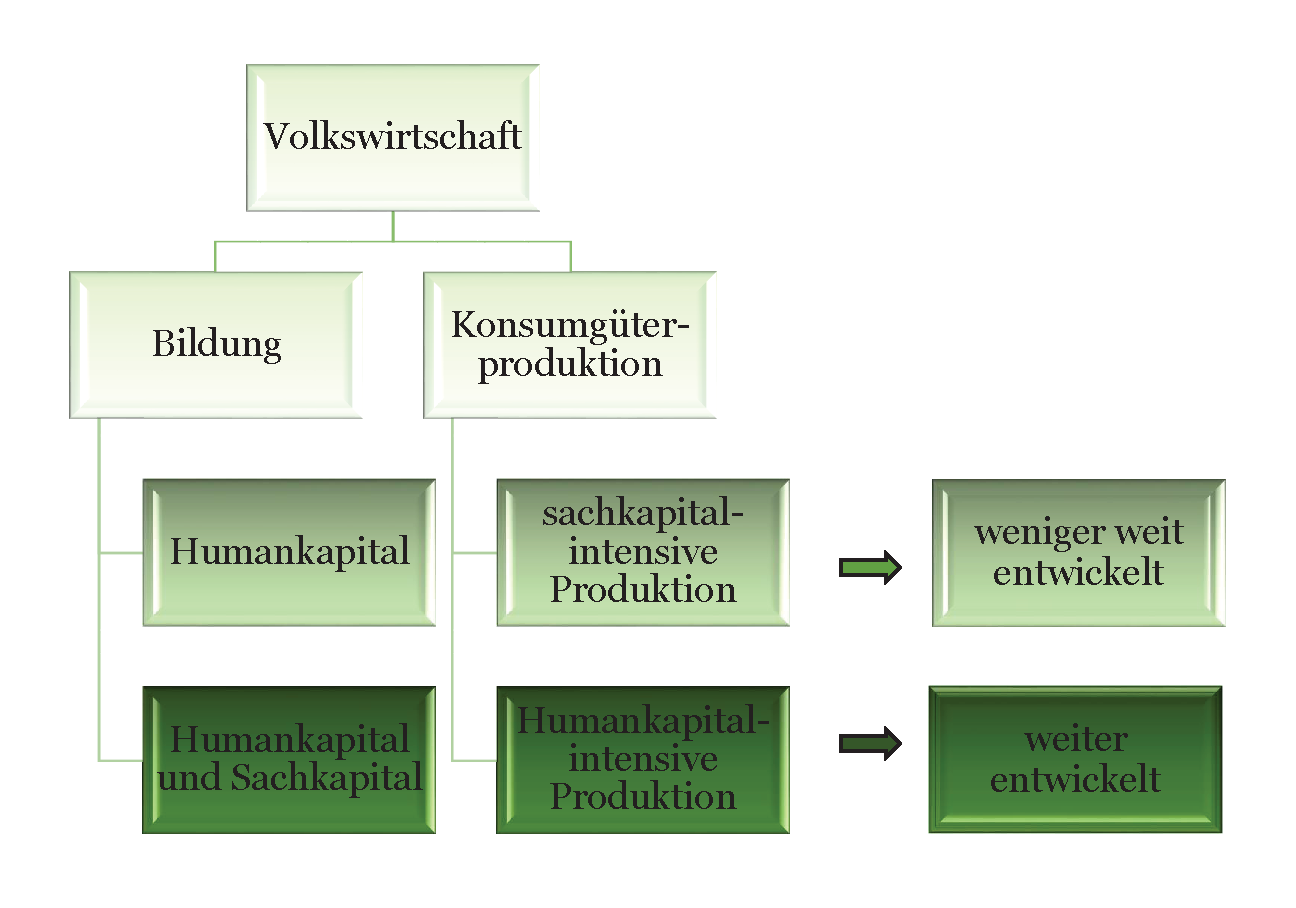
\includegraphics[width=0.7\textwidth]{C:/Users/BibiKiBa/Diss/Doktorarbeit/ModellEins/Abbildungen/SchemaPapierZwei.eps}
	\hfill\quelle{\textbf{Quelle:}}  ENTWURF! eigene Darstellung
	\caption{Kategorisierung der Entwicklungsstufen}
	\label{fig:SchemaPapierZwei}		
\end{figure*}
%
In einer ökonomisch kleinen Volkswirtschaft gibt es die beiden Sektoren Güterproduktion und Bildung. Im Konsumgutsektor wird ein Gut produziert, hier die Handtasche, die einem repräsentativen Haushalt einen Nutzen stiftet. Der Nutzen besteht in diesem Fall aus der Bedürfnisbefriedigung etwas von einem Ort zu einem anderen transportieren zu können. Für die Herstellung des Gutes werden grundsätzlich physisches Kapital sowie auch Humankapital benötigt. Beide Produktionsfaktoren können jedoch gegeneinander substituiert werden und das Gut kann je nach Einsatzverhältnissen relativ sachkapitalintensiv oder humankapitalintensiv produziert werden. Auf das Beispiel bezogen bedeutet dies, dass eine Handtasche von speziell ausgebildeten Täschnern in Handarbeit hergestellt wird. Der Herstellungsprozess ist sehr aufwendig, detailorientiert und erfordert besondere Fähigkeiten und Fertigkeiten. Diese qualifizierte Arbeit ist sehr knapp und wird dementsprechend hochpreisig entlohnt. Ein konkretes Beispiel ist die in Frankreich gefertigte Birkin Bag der Marke Hermes, bei der weltweit nur wenige Menschen in der Lage sind diese mit den entsprechenden Qualitätsanforderungen herzustellen.\\
%
Jedoch kann eine Handtasche den gleichen Zweck erfüllen, wenn ihr Produktionsprozess durch weniger qualifizierte Arbeit und deutlich stärkeren Maschineneinsatz geprägt ist.
Ein Land wie beispielsweise Bangladesch, das spezialisiert ist auf die Textilindustrie, weist zwar eine relativ hohe Ausstattung an Arbeit vor, jedoch mit geringfügigeren Qualifikationen als Frankreich. Ein Großteil der arbeitenden Bevölkerung dieser Branche wird eine Industrienähmaschine bedienen können und auch weitere handwerkliche Fähigkeiten haben, jedoch sind die Arbeitsabläufe stark durch Arbeitsteilung geprägt und ein umsichtig allumfassender Überblick sowie eine fachkundige Einschätzung des Herstellungsprozesses fehlt. Der Schwerpunkt liegt dann auf der starken Spezialisierung jedes einzelnen Arbeiters auf einfache Arbeitsschritte, ohne dabei jedoch andere Fähigkeiten zu fördern. Somit können auch die Folgen und Konsequenzen einer Neuerung schlecht eingeschätzt werden. 
Neben der Unterscheidung des Produktionsprozesses im Konsumgütersektor wird auch der Bildungssektor hinsichtlich der Einsatzfaktoren differenziert. So besteht grundsätzlich die Möglichkeit nur durch den Einsatz von Lehrkräften, hier bereits ausgebildete Schneider, die Fähigkeiten auf weniger qualifizierte Arbeiter auszuweiten. 
Ebenfalls denkbar ist neben dem Einsatz von Lehrkräften ein zusätzlicher Einsatz von Sachkapital wie Nähmaschinen, Bücher oder Lehrvideos.\\
%
Auf Grundlage dieser Differenzierungsmöglichkeiten werden in diesem Kapitel verschiedene Entwicklungsstadien unterschieden. Demzufolge wird in einem relativ weniger weit entwickelten Land tendenziell mehr Sachkapital als Humankapital vorhanden sein und entsprechend die Produktionsstruktur diesem Umstand angepasst, also relativ sachkapitalintensiv produzieren. Hinzu kommt, dass meist auf den Einsatz von physischem Kapital im Bildungssektor verzichtet wird.\\
%
Bei einem relativ weiter entwickeltem Land wird angenommen, dass relativ gesehen mehr Humankapital als Sachkapital vorhanden ist, verglichen mit einem Land oder Region, das weniger weit entwickelt ist. Dies führt zu einer humankapitalintensiven Produktion im Konsumgutsektor und zu einer Optimierung des Bildungssektors durch den Einsatz beider Produktionsfaktoren. 

\section{Autarkie}
Zunächst wird die Situation ohne Handel betrachtet. Es wird ebenfalls ein zwei Sektor-Modell vorgestellt, dass sich noch stark an der Arbeit von \cite{Lucas.1988} orientiert. Bei dem einen Sektor handelt es sich um einen Konsum- bzw. Investitionsgutsektor bei dem anderen um den Bildungssektor.
%
\subsection*{Produktion}
In dem vorliegenden Modell einer geschlossenen Volkswirtschaft können die beiden Produktionsfaktoren physisches Kapital $K(t)$ und Arbeit $L(t)$ für den Konsumgut- oder Bildungssektor verwendet werden. 
Dabei wird angenommen, dass sich die Faktoren frei zwischen den beiden Sektoren bewegen können und demzufolge keine Anforderungen erfüllen müssen, um in den anderen Sektor zu wechseln. Die Mobilität der Faktoren führt zu einem Ausgleich der Faktorpreise \cite{Samuelson.1941}. Für physisches Kapital muss ein Zinssatz $r$ an die Kapitalgeber entrichtet werden und die Arbeiter erhalten den Lohnsatz $w$. Dabei ist der Preis für die Arbeit $w$ exogen gegeben und steigt nicht mit zusätzlicher Bildung an. Der Faktor Arbeit hängt von der Bevölkerungsgröße $N(t)$ eines Landes ab sowie vom durchschnittlichen Humankapitalbestand $h(t)$ und dem Anteil des Humankapitals $u(t)$, der in die Produktion des Konsumgutsektors eingeht.
%
\begin{equation}
	L(t)=N(t)u(t)h(t)
	\label{eq:Arbeit}
\end{equation}
%
Das physische Kapital setzt sich zusammen aus dem durchschnittlichen Kapitalbestand $k(t)$ und dem Anteil des physischen Kapitals $v(t)$, der ebenfalls bei der Produktion des Konsumgutes verwendet wird. 

%
\begin{equation}
	K(t)=v(t)k(t)
	\label{eq:Kapital}
\end{equation}
%
Die Produktionsfunktionen sind linear homogen und demnach liegen konstante Skalenerträge vor. Bei der Konsumgüterproduktion führt der erhöhte Einsatz von Produktionsfaktoren zu einem proportionalen Anstieg der Ausbringungsmenge.
%
\begin{equation}
	\text{Konsumgutsektor:}\qquad F[K,L]= A(v(t)k(t))^\alpha(u(t)h(t))^{1-\alpha}
	\label{eq:ProduktionsfunktionK}
\end{equation}
%
Das Gut kann abhängig von der Produktionselastizität $\alpha$ mit relativ viel physischem Kapital oder Humankapital produziert werden. Demnach kann die Handtasche durch vollständige Eigenleistung von qualifizierten Täschnern hergestellt werden, oder durch den verstärkten Einsatz von Maschinen bspw. während des Zuschneideprozesses.\\
%
Im Bildungssektor bedeutet konstante Skalenerträge, dass jede zusätzliche Einheit Bildung zu dem gleichen Lernerfolg führt.\footnote{Diese Annahme weicht insofern von der Realität ab, als das Bildung einen abnehmenden Grenzertrag aufweisen kann. Der zusätzliche Nutzen des "`Addierens"' und "`Subtrahierens"' ist höher als eine "`Wurzel ziehen"' zu können. Deshalb wird auf gesamtwirtschaftlicher Ebene weiterhin von abnehmenden Grenzerträgen ausgegangen, jedoch nicht auf der Ebene des Haushalts, der hier den Nutzen maximiert.} 

%
\begin{equation}
	\text{Bildungssektor:} \qquad G[K,L]= B((1-v(t))k(t))^{\eta}((1-u(t))h(t))^{1-\eta}
	\label{eq:ProduktionsfunktionH}
\end{equation}
%
Ebenso kann der Bildungssektor erweitert werden, durch den Einsatz von relativ viel physischem Kapital, wenn die Produktionselastizität $\eta$ hoch ist, oder eher humankapitalintensiv, wenn $\eta$ gering ist. Auch im Lernprozess spielt das Einsatzverhältnis eine Rolle. Angenommen es wird einer Gruppe von Schneiderlehrlingen durch die Lehrkraft an einem Beispiel mit nur einer Nähmaschine ein Prozess vorgeführt, ist der Lernerfolg ein anderer, als wenn jeder einzelne die Möglichkeit hat an einer eigenen Nähmaschine die neue Technik beliebig oft zu wiederholen und zu üben. \\
%
Die Aufteilung der Produktionsfaktoren auf die Sektoren wird dargestellt durch die Anteile $u(t)$ bzw. $v(t)$. Das physische Kapital wird im Konsumsektor verwendet mit $v(t)$ und im Bildungssektor mit $(1-v(t))$. Um das Beispiel der Textilindustrie aufzugreifen, wäre physisches Kapital bei der Produktion einer Handtasche die Nadel, bzw. die Nähmaschine. Dieses kann entweder dazu verwendet werden tatsächlich Güter zu produzieren, oder aber um die Qualifikationen zu erweitern und den Lernprozess zu beschleunigen, indem man das neu gewonnene Wissen direkt anwendet. Ganz ähnlich erfolgt die Aufteilung des Humankapitals. Der Anteil $u(t)$ des Humankapitals wird für die Herstellung des Konsumgutes eingesetzt, wohingegen $(1-u(t))$  in den Bildungssektor eingeht. Auch hier kann das Wissen eines Einzelnen über die Zuschnitttechniken oder Säuberungsarbeiten  bei der Herstellung des Gutes eingesetzt werden, oder als Multiplikator im Bildungssektor, indem das vorhandene Wissen an bislang Unwissende weiter getragen wird.
%
\subsection*{Konsum}
Die Gesamtheit aller Haushalte richtet sich nach der Bevölkerungsgröße eines Landes, die mit der exogenen Rate $n$ über die Zeit $t$ wächst und von der anfänglichen Bevölkerungsgröße $N_0$ ausgeht.  
%
\begin{equation}
	N(t)=N_0e^{nt}
	\label{eq:Bevolkerungsentwickung}
\end{equation}
%
Die von den Unternehmen nachgefragten Produktionsfaktoren physisches Kapital und Humankapital bieten die Haushalte über die Faktormärkte an. Sie haben die Wahl die Konsumgüter zu verbrauchen oder diese in zukünftigen Konsum zu investieren, also zu sparen und dadurch Kapital zu akkumulieren. 
Es wird angenommen, dass alle Haushalte die gleichen Präferenzen haben und sie ihren Nutzen intertemporal maximieren. Auch hier wird von der Symmetrie der Haushalte ausgegangen und sie diskontieren ihren zukünftigen Nutzen mit der gleichen Rate, $\rho$. Der zukünftige Nutzen ist ihnen weniger wert, als der heutige Nutzen, demnach gilt, dass $\rho>0$. 
%
\begin{equation}
	V=\int \limits_{0}^\infty  \! e^{-\rho t}\psi(c(t)) \, dt
\end{equation}
%
Der angeführte Lebenszeitnutzen $V$ bei einem unendlichen Zeithorizont ergibt sich aus der Gesamtheit aller jeweils gegenwärtigen Nutzenwerte zu den verschiedenen Zeitpunkten. Die Zeitpunkte sind additiv separabel miteinander verknüpft. Demnach wird der aus dem Konsum resultierende Nutzen in jedem Zeitpunkt neu bewertet und wird unabhängig von der Bewertung zu einem anderen Zeitpunkt sein.
%
\begin{equation}
	\psi(c(t))=\frac{c(t)^{1-\sigma}}{1-\sigma}
\end{equation} 
%
Der gegenwärtige Nutzen der Haushalte $\psi(t)$ ist nur von der konsumierten Menge der Güter $c(t)$ abhängig, nicht vom Bildungsniveau. Außerdem ist der Konsum zwischen den Zeitpunkten intertemporal variabel, in welchem Ausmaß der Konsum zwischen zwei Zeitpunkten substituiert werden kann, hängt von der intertemporalen Substitutionselastizität $\sigma$ ab.\\
%
Die Maximierung des intertemporalen Nutzens lässt die Haushalte einen optimalen Konsumpfad wählen. Dabei müssen sie sich entscheiden zwischen dem Konsum  des Gutes oder der Investition in den Kapitalstock. Hinzu kommen die Entscheidungen hinsichtlich der Aufteilung des physischen Kapitals und Humankapitals auf die beiden Sektoren, welche Aussagen über die Präferenzen der Haushalte, bezüglich des Konsums und der Bildung zulässt. Demzufolge sind die Entscheidungsvariablen des folgenden Maximierungsproblems die Konsummenge $c(t)$, der Anteil des physischen Kapitals, der in die Produktion des Konsumgutes eingeht $v(t)$ und darüber gleichzeitig den Humankapitalsektor determiniert, wegen $(1-v(t))$, sowie der Aufteilung des Humankapitals durch $u(t)$ auf die beiden Sektoren.\\
%
Die dynamische Betrachtung des zu maximierenden Lebenszeitnutzens $V$ verläuft über den Zeithorizont von $0$ bis $\infty$ und beginnt mit den Anfangswerten des Kapitals $k_0$ und $h_0$.\footnote{Die beiden Startwerte $k_0$ und $h_0$ sind exogen.}
%
\begin{equation}\operatorname*{max}_{c(t),u(t),v(t)}V[k_0,h_0]= \int_{0}^\infty e^{-\rho t} \frac{c(t)^{1-\sigma}}{1-\sigma}dt\end{equation}
%

Der Nutzen wird nur dann maximal, wenn die beiden Veränderungen der Kapitalstöcke über die Zeit berücksichtigt werden. Denn durch jede zusätzliche Einheit Kapital verändert sich der Lebenszeitnutzen. Durch einen gegenwärtigen Aufbau eines Kapitalstocks kann zukünftig mehr Nutzen generiert werden. Es besteht also eine direkte Abhängigkeit zwischen den Bewegungsgleichungen von Sach- und Humankapital, $\dot{k}$ und $\dot{h}$, sowie dem Lebenszeitnutzen.
%
\begin{equation}\dot{k}(t)=A(v(t)k(t))^\alpha(u(t)h(t))^{1-\alpha}-c(t)\end{equation}
%
\vspace{-0.8cm}
	\begin{equation} \dot{h}(t)=B((1-v(t))k(t))^{\eta}((1-u(t))h(t))^{1-\eta}\end{equation}
%

		\vspace{-0.3cm}
		\begin{displaymath} c(t)\geq 0,\quad k(t)\geq 0,\quad h(t)\geq 0, \end{displaymath}
	\begin{displaymath} 0\leq u(t)\leq 1,\quad 0\leq v(t) \leq1, \end{displaymath}
\begin{displaymath} 0\leq \alpha\leq 1,\quad 0\leq \eta \leq1, \quad A\geq 0, \quad B\geq 0\end{displaymath}
%
Das Sachkapital erhöht sich durch all die produzierten Güter, die nicht konsumiert werden. Der Produktion der Güter dient sowohl physisches Kapital als auch Humankapital. Bei $A$ handelt es sich um einen Technologieparameter, der das technische Wissen im Konsumgutsektor berücksichtigt. Humankapital wird ebenfalls durch beide Kapitalarten aufgebaut und durch den Technologieparameter $B$ beeinflusst. Dabei gehen die Produktionsfaktoren jeweils mit einer Produktionselastizität von $\alpha$ bzw. $\eta$ in den jeweiligen Prozess ein.\\
%
Da es sich um ein intertemporales Optimierungsproblem handelt, ist es mit der Hamilton Funktion zu lösen. Dieses Verfahren wird auch Maximumprinzip genannt und geht zurück auf \cite{Pontryagin.1964}. Es beschreibt den optimalen Konsumpfad, der den Lebenszeitnutzen, unter Berücksichtigung der Entscheidungen der Haushalte über $c(t)$, $u(t)$ und $v(t)$ maximiert. Diese Entscheidungsvariablen determinieren die zukünftige Ausweitung der Kapitalstöcke $k(t)$ und $h(t)$. Es besteht zu jedem Zeitpunkt eine Abhängigkeit des Lebenszeitnutzens zu dem jeweils gegenwärtig vorhandenem physischen Kapitalstock und Humankapitalstock, sowie zu den Entscheidungen des Haushalts über die Aufteilung der Ressourcen auf die beiden Sektoren.\footnote{Ressourccen eines Haushalts können die Zeit, Kraft oder auch die Konzentration sein.} Deshalb sind für die Lösung des dynamischen Maximierungsproblems die Bewegungsgleichungen von $h(t)$ und $k(t)$ notwendig, da diese die jeweilige Veränderung der Kapitalstöcke über die Zeit beschreiben.\footnote{Aus Gründen der Anschaulichkeit wird im folgenden die Abhängigkeit der Variablen gegenüber der Zeit $t$ vernachlässigt.}
%
\begin{equation}
	\begin{split}
		\mathbb{H}=&~e^{-\rho t}\frac{c^{1-\sigma}}{1-\sigma}\\
%
		&+\gamma_1(A(vk)^\alpha(uh)^{1-\alpha}-c)\\
%
		&+\gamma_2B[(1-v)k]^{\eta}[(1-u)h]^{1-\eta}\\
%
	\end{split}
\end{equation}
%
\begin{displaymath}
	\gamma_1 > 0,\quad \gamma_2 > 0
\end{displaymath}
%
Die Optimierung über die Hamiltonfunktion gibt Auskunft über den resultierenden Gesamtnutzen für die anberaumte Lebenszeit. Außerdem ist ein Vergleich resultierender Nutzwerte zweier aufeinanderfolgender Zeitpunkte möglich. Der erste Summand beschreibt den gegenwärtigen Nutzeneffekt herbeigeführt durch den Konsum von Gütern, der wiederum über die Entscheidungsvariablen determineirt wird. Die folgenden Summanden der Hamiltonian stellen die zukünftigen Nutzeneffekte der zukünftigen Veränderungen des Sach- und Humankapitals dar, dessen gegenwärtige Nutzwerte durch die zugehörigen Schattenpreise $\gamma_1$ und $\gamma_2$ ausgedrückt werden.\footnote{Bei den Variablen $\gamma_1$ und $\gamma_2$ handelt es sich originär um Hilfsvariablen oder auch als Schlupfvariablen bekannt, die hier als Schattenpreis interpretiert werden können.} Die Schattenpreise ergeben sich aus der Ableitung des Lebenszeitnutzens nach jeweils einem Produktionsfaktor und sind somit der Lebenszeitgrenznutzen einer Einheit Sach- oder Humankapital. Dieser drückt den Wert einer zusätzlichen Einheit Kapital für den gesamten Zeithorizont aus, also eine mögliche marginale Lebenszeitnutzenverbesserung durch eine zusätzliche Einheit Kapital.  Beide Schattenpreise sind positiv, da ansonsten eine Einsatzfaktoränderung zu einer Indifferenz der Haushalte führt. Denn bei einem Schattenpreis von Null würde der zukünftige Nutzen den Lebenszeitnutzen nicht tangieren und der Fokus auf der Gegenwart liegen ohne zukünftige Zeitpunkte zu berücksichtigen. Durch die Multiplikation mit dem Schattenpreis wird der Nutzwert der Kapitalerhöhung berücksichtigt. Der Schattenpreis "`konvertiert"' die Faktoreinheiten in Nutzeinheiten unter Berücksichtigung der zeitlichen Veränderung. Beide Nutzeneffekte konkurrieren miteinander, da ein gegenwärtiger Konsum den zukünftigen mindert \cite{Chiang.2000,Chiang.2011}.\\
% 
Diese Optimierung findet für alle möglichen Zeitpunkte statt und ermöglicht eine Vergleichbarkeit zweier aufeinanderfolgender Zeitpunkte. Erst dann wenn der heutige Grenznutzen mit dem morgigen übereinstimmt, wurde der optimale Konsumpfad einer Volkswirtschaft gefunden \cite{Chiang.2000}. Folgende Bedingungen erster Ordnung lösen das Optimierungsproblem.\footnote{Die ausführliche Berechnung aller Gleichgewichtsbedingungen sind in Appendix \ref{AutarkieAPPENDIX} zu finden.}  
%
\begin{align}
	&\frac{\partial\mathbb{H}}{\partial c}\overset{!}{=}~0\label{eq:foc1WM}\\
	%
	&\frac{\partial\mathbb{H}}{\partial v}\overset{!}{=}~0\label{eq:foc2WM}\\
	%
	&\frac{\partial\mathbb{H}}{\partial k}\overset{!}{=}-\dot{\gamma_1}\label{eq:foc3WM}\\
	%
	&\frac{\partial\mathbb{H}}{\partial u}\overset{!}{=}~0\label{eq:foc4WM}\\
	%
	&\frac{\partial\mathbb{H}}{\partial h}\overset{!}{=}-\dot{\gamma_2}\label{eq:foc5WM}
\end{align}
%
Die Bedingungen erster Ordnung werden im Folgenden recht allgemein, jedoch sehr ausführlich beschrieben, um in der folgenden Analyse hinsichtlich verschiedener Entwicklungsstände größtenteils darauf verzichten zu können. 
\subsubsection*{Ableitung nach Zustandsvariablen, $k$ und $h$}
Die Ableitung nach einer Zustandsvariablen wird mit der jeweiligen negativen Bewegungsgleichung des Schattenpreises gleichgesetzt.\footnote{Der Lebenszeitgrenznutzen einer zusätzlichen Einheit $\gamma$ ist zwar positiv, jedoch abnehmend mit zunehmendem Kapitaleinsatz über die Zeit. Demzufolge ist die Ableitung des Schattenpreises nach der Zeit negativ. Das negative Vorzeichen gleicht diesen Zusammenhang aus und es kann eine Gleichheit beider Seiten herbeigeführt werden.} Dabei handelt es sich um eine intertemporale Arbitragebedingung, die gleich dem jeweiligen negativen Lebenszeitgrenznutzen sein soll. Die Abnahme des Schattenpreises über die Zeit $\dot{\gamma}$ kann auch als Abschreibungsrate des Schattenpreises interpretiert werden und soll genau so groß sein, wie die Erhöhung des gegenwärtigen und zukünftigen Nutzen durch die Kapitalakkumulation. Erst wenn sich beide Größen ausgeglichen haben, kann der Lebenszeitnutzen maximal sein \cite{Chiang.2000,Chiang.2011}.
%
\subsubsection*{Ableitung nach Entscheidungsvariablen $v$,$u$ und $c$ }
Die Ableitung nach einer Zustandsvariablen ergibt die optimale Allokation eines Produktionsfaktors in jedem Sektor zu jedem Zeitpunkt. Die Gleichsetzung der Ableitung einer Entscheidungsvariablen mit $0$ bedeutet, dass dann diese Variable maximal sein wird, unter der Voraussetzung, dass die Bedingung der jeweils zugehörigen Zustandsvariablen erfüllt ist.\\
%
Die Entscheidungsvariable wird direkt vom Wirtschaftssubjekt gewählt, aus ihr ergibt sich dann indirekt die Zustandsvariable \cite{Chiang.2011}. Die Haushalte entscheiden sich sowohl für den Konsum, als auch für die Aufteilung der eigenen Ressourcen, die ihren Nutzen maximieren. Dabei muss, um beim anfänglichen Beispiel zu bleiben, berücksichtigt werden, wie viele Handtaschen sie derzeit konsumieren möchten und wie viel Sachkapital, wie Nadeln, Nähmaschinen oder Scheren  sie bereit sind für die Produktion bzw. für ihre Weiterbildung zu den unterschiedlichen Zeitpunkten zu investieren. 
%
\subsubsection*{Ableitung nach $c$}
Durch die Ableitung der Hamiltonian nach dem Konsum $c$, siehe \colorbox{lightgray}{Gleichung \eqref{eq:foc1WM}}, wird der maximale Konsum unter Berücksichtigung der Nebenbedingungen $\dot{k}$ und $\dot{h}$ bestimmt.
%
\begin{equation}
	\colorbox{lightgray}{$\partial\mathbb{H}/\partial c\overset{!}{=}~0$}
\end{equation}
%
\vspace{-0.5cm}
%
\begin{equation}
	e^{-\rho t}c^{-\sigma}-\gamma_1 = 0
\end{equation}
%
\vspace{-0.7cm}
%
\begin{equation}
	\gamma_1=e^{-\rho t}c^{-\sigma}
	\label{eq:foc1WMa}
\end{equation}
%
Die Gleichung \eqref{eq:foc1WMa} drückt aus, dass der diskontierte Grenznutzen des optimalen Konsums pro Kopf gleich dem gegenwärtigen Schattenpreis $\gamma_1$ einer zusätzlichen Sachkapitaleinheit ist. Da auch die zweite Ableitung nach $c$ kleiner $0$ ist, handelt es sich um einen maximalen Punkt. 
%
\begin{equation}
	-e^{-\rho t}\sigma c^{-\sigma-1}<0
\end{equation}
%
Der Schattenpreis beschreibt in diesem Fall wie hoch die Lebenszeitnutzenerhöhung ist, wenn auf den heutigen Konsum verzichtet wird und welchen zukünftigen Nutzenwert die  daraus resultierende Kapitalakkumulation stiften wird.\\
%
Die optimale Konsumgütermenge beeinflusst im Wesentlichen die Sachkapitalakkumulation. Die Entscheidung des Haushalts über die gegenwärtige Konsummenge an Handtaschen bedingt die Akkumulation von Handtaschen und den damit verbundenen Güterberg. Denn je mehr konsumiert wird, desto weniger Gütereinheiten können in die Kapitalakkumulation investiert werden. Demzufolge ist für die weitere Analyse eine Ableitung der Zustandsvariablen $k$ notwendig.
% 
\subsubsection*{Ableitung nach $k$}
Bei der Variablen $k$ handelt es sich um eine Zustandsvariable, die den aus der Konsumentscheidung resultierenden Zustand angibt. Neben dem Konsum beeinflusst auch die Aufteilung des Sachkapitals auf die beiden Sektoren $v$ den Kapitalbestand. Steigt der Kapitalstock um eine Einheit an, dann erhöht sich der Lebenszeitnutzen um den Schattenpreis, der den Wert dieser zusätzlichen Kapitaleinheit in Nutzeneinheiten angibt. Diese Auswirkung auf den Nutzen durch die Veränderung einer Einheit Sachkapital beschreibt \colorbox{lightgray}{Gleichung \eqref{eq:foc3WM}}. Der gegenwärtige Grenznutzen des physischen Kapitals soll also dem zukünftigen Nutzen einer Einheit Sachkapital entsprechen. Der Einsatz einer zusätzlichen Nähmaschine führt im Konsumgütersektor zu einer erhöhten Produktion von Handtaschen, die entweder für den Eigenbedarf genutzt werden können oder aber den Kapitalstock erhöhen. Es besteht jedoch auch die Möglichkeit die Sachkapitaleinheit in den Bildungssektor für das Erlernen neuer effizienterer Nähtechniken zu investieren. In beiden Fällen erhöht sich der Lebenszeitnutzen, entweder durch den gegenwärtigen oder durch den zukünftigen Konsum. Die Höhe des zusätzlichen künftigen Nutzens wird am Schattenpreis bemessen. So gilt für die erste Ableitung der Hamiltonian nach dem physischen Kapital $k$, dass diese im Gleichgewicht der negativen ersten Ableitung nach der Zeit des Schattenpreises von Sachkapital entspricht. 
%
\begin{equation}
	\colorbox{lightgray}{$\partial\mathbb{H}/\partial k\overset{!}{=}-\dot{\gamma_1}$}\label{nachK}
\end{equation}
%
\begin{equation}
	\gamma_{1}A v^{\alpha}k^{\alpha -1} \alpha(u h)^{1- \alpha} + \gamma_{2}B(1- v)^{\eta} k^{\eta -1} \eta \left [ (1-u)h \right ]^{1- \eta}\overset{!}{=} - \dot{\gamma}_{1}\label{BedingungFoc3WM}
\end{equation}
%
Der gegenwärtige Nutzwert der auf Human- und Sachkapitalakkumulation zurückzuführen ist, soll dem zukünftigen Nutzwert entsprechen. Der Schattenpreis $\gamma_1$ wird mit der Rate abgeschrieben, mit der die künftige Kapitalakkumulation zur Lebenszeitnutzenerhöhung beiträgt. Erst wenn diese Bedingung erfüllt ist kann der Nutzen maximal sein \cite{Chiang.2000}.
%
\subsubsection*{Ableitung nach $v$}
Bei der Aufteilung des Sachkapitals den Konsumgutsektor und den Bildungssektor $v$, handelt es sich ebenfalls um eine Entscheidungsvariable. Indem eine marginale Veränderung dieser Aufteilung auf den Nutzen gleich null gesetzt wird, kann der Nutzen maximiert werden, sofern die Bedingung gemäß Gleichung \eqref{BedingungFoc3WM} erfüllt ist.
Wird die allgemeine Form aus \colorbox{lightgray}{Gleichung \eqref{eq:foc2WM}} hier konkret ausformuliert ergibt sich:
%
\begin{equation}
	\colorbox{lightgray}{$\partial\mathbb{H}/\partial v\overset{!}{=}~0$}
\end{equation}
%
\vspace{-0.5cm}
%
\begin{equation}
	\gamma_1A\alpha v^{\alpha-1}k^\alpha(uh)^{1-\alpha}-\gamma_2B\eta(1-v)^{\eta-1}k^\eta[(1-u)h]^{1-\eta}\overset{!}{=}~0
\end{equation}
%
\vspace{-0.7cm}
%
\begin{equation}
	\gamma_1A\alpha v^{\alpha-1}k^\alpha(uh)^{1-\alpha}=\gamma_2B\eta(1-v)^{\eta-1}k^\eta[(1-u)h]^{1-\eta}
\end{equation}
%
Demzufolge sollen sich die mit dem Schattenpreis bewerteten Grenzprodukte entsprechen. Eine zukünftige marginale Veränderung von $u$ bedingt im Konsumgutsektor einen anteilig höheren Einsatz von Sachkapital um den der Anteil im Bildungssektor dadurch reduziert wird. Der resultierende zusätzliche Nutzen des Kapitaleinsatzes im Konsumgutsektor soll die Minderung des Nutzens im Bildungssektor ausgleichen. Durch den Einsatz einer Nähmaschine in der Textilindustrie kommt es zu einer Nutzensteigerung, die genau der Nutzenminderung im Bildungssektor entsprechen muss. 
%
\subsubsection*{Ableitung nach $h$}
Auch im Bildungssektor soll sich die Veränderung der Lebenszeitgrenznutzen zweier aufeinanderfolgender Perioden entsprechen. Diesen Zusammenhang beschreibt \colorbox{lightgray}{Gleichung \eqref{eq:foc5WM}}. Der Grenznutzen des Humankapitals beschreibt eine Veränderung der Hamiltonian durch einen Anstieg um eine Einheit Humankapital und soll heute genau soviel Nutzen stiften wie in der folgenden Periode.
%
\begin{equation}
	\colorbox{lightgray}{$\partial\mathbb{H}/\partial h\overset{!}{=}-\dot{\gamma_2}$}\label{nachH}
\end{equation}
%
\begin{equation}
	\gamma_1A(1-\alpha)(vk)^\alpha u^{1-\alpha}h^{-\alpha}+\gamma_2 B(1-\eta)[(1-v)k]^{\eta}(1-u)^{1-\eta}h^{-\eta}\overset{!}{=}-\dot{\gamma}_2\label{GNHK}
\end{equation}
%
Dies ist genau dann erfüllt, wenn der zukünftige Nutzenwert der zusätzlichen Humankapitaleinheit dem heutigen Grenznutzen entspricht, da der Schattenpreis mit einer Rate von $-\gamma_2$ abgeschrieben wird. Der gegenwärtige Nutzengewinn aus einer Einheit qualifizierter Arbeit entspricht dem zukünftigen Nutzen durch den Einsatz selbiger in den Bildungssektor. Es sollte demnach im Gleichgewicht keinen Unterschied machen, wann ein ausgebildeter Schneider eingesetzt wird. 
%
\subsubsection*{Ableitung nach $u$}
Ist die Bedingung \eqref{GNHK} erfüllt, dann kann $u$ so gewählt werden, dass die Hamiltonian zu jedem Zeitpunkt maximal ist, indem \colorbox{lightgray}{Gleichung \eqref{eq:foc4WM}} gilt.
%
\begin{equation}
	\colorbox{lightgray}{$\partial\mathbb{H}/\partial u\overset{!}{=}~0$}
\end{equation}
%
\vspace{-0.5cm}
%
\begin{equation}
	\gamma_1A(1-\alpha)(vk)^{\alpha}h^{1-\alpha}u^{-\alpha}-\gamma_2B(1-\eta)[(1-v)k]^\eta (1-u)^{-\eta} h^{1-\eta}\overset{!}{=}0
\end{equation}
%
\vspace{-0.7cm}
%
\begin{equation}
	\gamma_1A(1-\alpha)(vk)^{\alpha}h^{1-\alpha}u^{-\alpha}=\gamma_2B(1-\eta)[(1-v)k]^\eta (1-u)^{-\eta} h^{1-\eta}\label{foc4}
\end{equation}
%
Die Aufteilung führt zu einem maximalen Nutzen, wenn sich die zukünftigen Grenzprodukte beider Sektoren entsprechen. Eine Umverteilung des Humankapitals muss in beiden Sektoren die gleiche Nutzenveränderung herbeirufen. Dann verändert sich der Lebenszeitnutzen nicht mehr durch eine Umverteilung des Einsatzortes des ausgebildeten Täschners.
%
\subsubsection*{Transversalitätsbedingung}
Die Transversalitätsbedingungen sind begrenzende Bedingungen der Schattenpreise. Sie gewährleisten, dass zum angenommen Endzeitpunkt des geplanten Zeithorizonts der Bestand der Zustandsvariablen vollständig aufgebraucht oder deren Wert in Höhe der Schattenpreise zum Planungsendzeitpunkt gleich $0$ ist \cite{Chiang.2000}.
%Sie beschreiben den Zeithorizont der zu treffenden Entscheidungen, hier über den Konsum, die Aufteilung des physisches Kapital und Humankapitals auf die beiden Sektoren.
%
\begin{equation}
	\lim_{t \to \infty}e^{-\rho t}\gamma_1k=0
\end{equation}
%
\vspace{-0.7cm}
%
\begin{equation}
	\lim_{t \to \infty}e^{-\rho t}\gamma_2h=0
\end{equation}
%
\subsection*{Gleichgewichtsbedingungen}
Fasst man die zuvor separat erläuterten Bedingungen zusammen, dann ergibt sich ein Gleichungssystem, welches die notwendigen Bedingungen beschreibt, damit eine autarke Volkswirtschaft langfristig im Gleichgewicht ist. 
%
\begin{align}
	&\gamma_1=e^{-\rho t}c^{-\sigma}\\
	%
	&\gamma_1A\alpha v^{\alpha-1}k^\alpha(uh)^{1-\alpha}=\gamma_2B\eta(1-v)^{\eta-1}k^\eta[(1-u)h]^{1-\eta}\\
	%
	&\gamma_{1}A v^{\alpha}k^{\alpha -1} \alpha(u h)^{1- \alpha} + \gamma_{2}B(1- v)^{\eta} k^{\eta -1} \eta \left [ (1-u)h \right ]^{1- \eta}= - \dot{\gamma}_{1}\label{foc3IL}\\
	%
	&\gamma_1A(1-\alpha)(vk)^{\alpha}h^{1-\alpha}u^{-\alpha}=\gamma_2B(1-\eta)[(1-v)k]^\eta (1-u)^{-\eta} h^{1-\eta}\\
	%
	&\gamma_1A(1-\alpha)(vk)^\alpha u^{1-\alpha}h^{-\alpha}+\gamma_2 B(1-\eta)[(1-v)k]^{\eta}(1-u)^{1-\eta}h^{-\eta}=-\dot{\gamma}_2
\end{align}
%
\vspace{-0.7cm}
%
\begin{equation}
	\lim_{t \to \infty}e^{-\rho t}\gamma_1k=0
\end{equation}
%
\vspace{-0.7cm}
%
\begin{equation}
	\lim_{t \to \infty}e^{-\rho t}\gamma_2h=0
\end{equation}
%
Aus diesen Bedingungen lässt sich, wie in Appendix \ref{AutarkieAPPENDIX} dargestellt, das gleichgewichtige Wachstum herleiten. 
%
\subsubsection*{Keynes-Ramsey-Regel}
Die Keynes-Ramsey-Regel beschreibt in ihrer ursprünglichen Form die Beziehung zwischen dem Grenzprodukt des Kapitals und dem daraus resultierenden Wirtschaftswachstum.  
%
\begin{equation}
	\boxed{\hat{c}=\frac{1}{\sigma}\left(A\alpha \left(\frac{vk}{uh}\right)^{\alpha -1}-\rho\right)}\label{KRRWM}
\end{equation}
%
Je produktiver eine Einheit Sachkapital ist, desto höher ist die Wachstumsrate. Es besteht ein positiver Zusammenhang zwischen dem Grenzprodukt des physischen Kapitals $A\alpha \left(\frac{vk}{uh}\right)^{\alpha -1}$ und der Wachstumsrate. Wohingegen ein negativer bzw. inverser Zusammenhang zwischen selbiger Wachstumsrate und dem Diskontfaktor $\rho$ besteht.\footnote{Der Kehrwert der intertemporalen Substitutionselastizität $1/\sigma$ ist ebenfalls positiv mit der Wachstumsrate verknüpft. Je leichter man zwischen den Zeitpunkten substituieren kann, desto höher ist die Wachstumsrate.} 
Diese Gleichung lässt jedoch noch keine konkreten Aussagen über die tatsächliche Größe der Variablen zu. So ist noch immer unklar wie hoch $u$ oder auch $v$ gewählt werden muss, um zum gleichgewichtigen Wachstumspfad zu konvergieren. Ebenso verhält es sich mit den Zustandsvariablen $k$ und $h$, auch hier ist noch unbekannt wie groß diese im Gleichgewicht sind. Die Gleichgewichtswerte werden im folgenden Abschnitt \ref{sec:Modelldynamik} beschrieben, deren Berechnung ist ausführlich in Appendix \ref{AutarkieAPPENDIX} zu finden. 
%
\subsection*{Modelldynamik}\label{sec:Modelldynamik}
Gleichung \eqref{KRRWM} zeigt, wenn das Verhältnis $k/h$ und die Kapitalaufteilungen $u$ und $v$ konstant sind, dass dann der Konsum mit konstanter Rate wächst. 
Betrachtet man das Wachstum des physischen Kapitals, dann sind ebenfalls das Verhältnis beider Kapitalarten $k/h$ sowie die Aufteilungen $v$ und $u$ relevant. Hinzu kommt das Verhältnis des Konsums zum physischen Kapital $c/k$ bzw. $\chi$.\footnote{Ersetzt man $\chi=\frac{c}{k}$ ergeben sich zwei Schreibweisen für die Wachstumsrate des physischen Kapitals.} Erst wenn diese konstant sind, wächst das Sachkapital $k$ mit konstanter Rate.
%
\begin{equation}
	\hat{k}=Av^\alpha k^{\alpha-1}(uh)^{1-\alpha}-\frac{c}{k} \qquad \hat{=} \qquad
	\hat{k}=Av^\alpha k^{\alpha-1}(uh)^{1-\alpha}-\chi 
\end{equation}
%
Ganz ähnlich verhält es sich mit dem Humankapital. Hier müssen wieder $k/h$, $v$ und $u$ konstant sein, damit das Humankapitalwachstum konstant ist. 
%
\begin{equation}
	\hat{h}=B\left[(1-v)\frac{k}{h}\right]^{\eta}(1-u)^{1-\eta}
\end{equation}
%
Verkürzt durch $x_1=\frac{vk}{uh}$ und $x_2=\frac{(1-v)k}{(1-u)h}$ lassen sich diese Gleichungen auch schreiben als:
%
\begin{equation}
	\boxed{\hat{k}=Ax_1^\alpha \frac{uh}{k}-\chi}
\end{equation}
%
\begin{equation}
	\boxed{\hat{h}=Bx_2^\eta(1-u)}
\end{equation}
%
Es liegt nahe, dass im Steady-State gilt, dass $\hat{c}=\hat{k}=\hat{h}$ und somit die Wachstumsraten gleich groß sind, wenn $k/h$, $c/k$, $u$ und $v$ konstante Größen sind. 
%
Eine Volkswirtschaft befindet sich dann im Gleichgewicht, wenn sich die Verhältnisse der Grenzproduktivitäten beider Sektoren entsprechen, die sich aus den Gleichungen \eqref{eq:foc2WM} und \eqref{eq:foc3WM} herleiten lassen. Eine Umverteilung des Kapitals zwischen den Sektoren stellt im Gleichgewicht keinen Sektor besser als zuvor. 
%
\begin{equation}
	\boxed{\frac{1-\alpha}{\alpha}x_1=\frac{1-\eta}{\eta}x_2}
\end{equation}
%
Eine zusätzliche Sach- oder Humankapitaleinheit weist im Konsumgutsektor die gleiche Grenzproduktivität auf wie im Bildungssektor. Dies ist dann der Fall, wenn sich die Schattenpreisverhältnisse in beiden Sektoren entsprechen und somit das Verhältnis der Lebenszeitgrenznutzen in beiden gleich groß ist. Langfristig verhalten sich die Relationen $x_1$ und $x_2$ gleich und mit Hilfe der folgenden Gleichung \eqref{A5} können die Wachstumsraten $\hat{x}_1$ und $\hat{x}_2$ berechnet werden, die demnach im Gleichgewicht konstant sind. 
%
\begin{equation}
	\hat{x}_1=\hat{x}_2=0
\end{equation}
%
Zur Lösung des Gleichungssystems ist eine weitere Bedingung notwendig, die sich aus Gleichung \eqref{nachK} und \eqref{nachH} herleiten lässt. Diese drücken aus, dass zum einen die Rate des Lebenszeitgrenznutzens von Humankapital dem Grenzprodukt des Humankapitals entspricht. Zum anderen die Wachstumsrate des Schattenpreises des physischen Kapitals ebenso gleich dem Grenzprodukt des Kapitals im Konsumgutsektor ist. 
%
\begin{equation}
	\boxed{B(1-\eta)x_2^\eta=-\rho-\sigma\hat{c}-\alpha\hat{x}_1+\eta\hat{x}_2}\label{A5}
\end{equation}
%
Der Nutzen aus einer zusätzlichen Humankapitaleinheit im Bildungssektor ist gleich dem resultierenden Nutzen einer zusätzlichen Einheit Sachkapital, da $\rho-\sigma\hat{c}=\hat{\gamma_1}=-A\alpha x_1^{\alpha-1}$ gemäß Gleichung \eqref{foc3IL}.
Demzufolge ergibt sich folgendes Gleichungssystem, welches das Gleichgewicht beschreibt.
%
\begin{align}
	&\hat{k}=Ax_1^\alpha \frac{uh}{k}-\chi\label{GG1WM}\\
	%
	&\hat{h}=Bx_2^\eta(1-u)\label{GG2WM}\\
	%
	& x_1(1-\alpha)/\alpha =x_2(1-\eta)/\eta\label{GG3WM}\\
	%
	&\hat{c}=\frac{1}{\sigma}\left(A\alpha x_1^{\alpha -1}-\rho\right)\label{GG4WM}\\
	%
	&B(1-\eta)x_2^\eta=-\rho-\sigma\hat{c}-\alpha\hat{x}_1+\eta\hat{x}_2\label{GG5WM}
\end{align}
%
Mithilfe dieses Gleichungssystems können die gleichgewichtigen Werte der verschiedenen Variablen bestimmt werden. Durch die Auflösung nach den optimalen Werten für $x_1$ und $x_2$ wird die Konsumwachstumsrate umgeformt in:\footnote{Siehe Appendix \ref{AutarkieAPPENDIX}.} 
%
\begin{equation}
	\boxed{\hat{c}^*=\frac{1}{\sigma}\left(\left[A^\eta\alpha^{\alpha\eta}(1-\eta)^{(1-\eta)(1-\alpha)}(\eta(1-\alpha))^{\eta(1-\alpha)}B^{1-\alpha}\right]^\frac{1}{1+\eta-\alpha}-\rho\right)}
\end{equation}
%
Dabei hängt das Grenzprodukt $\left[A^\eta\alpha^{\alpha\eta}(1-\eta)^{(1-\eta)(1-\alpha)}(\eta(1-\alpha))^{\eta(1-\alpha)}B^{1-\alpha}\right]^\frac{1}{1+\eta-\alpha}$ von den Technologieparametern $A$ und $B$ beider Sektoren ab und wird im folgenden mit $M$ abgekürzt. Durch jeglichen technologischen Fortschritt erhöht sich das Wirtschaftswachstum.\\
%
Die gleichgewichtige Aufteilung des Humankapitals $u^*$ ist dadurch bedingt, dass im Gleichgewicht \colorbox{lightgray}{$\hat{c}=\hat{h}$} gilt.
%
\begin{equation}
	\boxed{u^*=\frac{\sigma M-(1-\eta)(M-\rho)}{\sigma M}}\label{uOptAut}
\end{equation}
%
Im wesentlichen existiert eine Abhängigkeit der Humankapitalaufteilung $u$ zum Grenzprodukt des Kapitals $M$. Zwischen beiden besteht eine inverse Beziehung, somit wird ein abnehmendes Grenzprodukt des Kapitals durch den erhöhten Einsatz von Humankapital in den Konsumgutsektor kompensiert. Wenn jede zusätzliche Nähmaschine im Konsumgutsektor nun weniger produktiv ist, als die zuvor Eingesetzte, wird die qualifizierte Arbeit nicht mehr im Konsumgutsektor zur Produktion eingesetzt, sondern stattdessen in den Bildungssekor investiert.  Je höher die Zeitpräferenz $\rho$ ist, desto weniger wird Humankapital in den Bildungssektor investiert. Zukünftige möglicherweise höhere Konsummöglichkeiten durch den Einsatz qualifizierterer Arbeit haben eine geringere Bedeutung, als der heutige Konsum. Demzufolge besteht ein positiver Zusammenhang zwischen der Diskontrate und dem Anteil des Humankapitals, der in die Konsumgüterproduktion eingeht. Diese Größe $u^*$ dient als Referenzwert und wird im folgenden die Wirkung der Offenheit verdeutlichen. 
Für das physische Kapital ergibt sich die folgende optimale Aufteilung im Gleichgewicht. 
%
\begin{equation}
	\boxed{%
		v^*=\frac{\alpha  (1-\eta ) \left(\frac{M}{B (1-\eta )}\right)^{1/\eta } (M \sigma -(1-\eta ) (M-\rho ))}{(1-\alpha ) \eta  M \sigma  \left(\frac{\alpha  (1-\eta ) \left(\frac{M}{B  (1-\eta )}\right)^{1/\eta } (M \sigma -(1-\eta ) (M-\rho ))}{(1-\alpha ) \eta  M \sigma }+\left(\frac{M}{B  (1-\eta )}\right)^{1/\eta } \left(1-\frac{M \sigma -(1-\eta ) (M-\rho )}{M \sigma }\right)\right)}%
		}
\end{equation}
%
Ebenso wie bei $u^*$ aus \eqref{uOptAut} besteht zwischen der Aufteilung des Sachkapitals $v$ und dem Grenzprodukt des Kapitals $M$ ein inverser Zusammenhang,
 sowie ein positiver zu der Diskontrate $\rho$. Je höher das Grenzprodukt ist, desto weniger physisches Kapital ist notwendig um das gleiche Outputniveau zu erzielen. Es müssen weniger Nähmaschinen eingesetzt werden, da nun jede Maschine produktiver ist. Das überschüssige Sachkapital wird nun in den Bildungssektor fließen und dort die Produktivität steigern. 
Die Relation des Konsums zum physischen Kapital $\chi$ kann durch \colorbox{lightgray}{$\hat{c}=\hat{k}$} ermittelt werden.
%
\begin{equation}
	\boxed{%
	\chi^*=\frac{1}{\sigma}\left(\frac{A\alpha \sigma[-\eta\rho+M(\eta+\sigma-1)+\rho] \left(\frac{\alpha  (\eta -1) \left(\frac{M}{B (1-\eta) }\right)^{1/\eta }}{(\alpha -1) \eta }\right)^{\alpha -1}}{\rho  (\alpha -\eta )+M (\alpha  (\sigma -1)+\eta )}-M+\rho\right)%
	}
\end{equation}
%
Basierend auf der goldenen Regel der Kapitalakkumulation kann $\chi$ als die Regel für die optimale Aufteilung der Kapitalakkumulation durch Ersparnisbildung, hier Konsumverzicht beschrieben werden, die das Pro-Kopf-Einkommen maximiert \cite{Nelson.1966}. Davon ausgehend, dass ein maximales Einkommen auch zu dem größtmöglichen und somit optimalen Konsum führt, kann das Prinzip der goldenen Regel der Kapitalakkumulation hier angewendet werden. Im Gleichgewicht existiert demnach eine konstante Kapital-Konsumquote $\chi$.
%
\section{Handel}
Wird die übrige Welt hinzugezogen, mit der Handel betrieben wird hinzugezogen, besteht die Notwendigkeit der Betrachtung eines weiteren Gutes. Dieses zweite Gut unterschiedet sich nur hinsichtlich der Faktoreinsatzverhältnisse vom ersten. Ansonsten erfüllt es den gleichen Nutzen und weist auch die gleichen Eigenschaften auf. 
Aufgrund der hierangeführten relativen Ausstattungsunterschiede ergibt sich folgende Handelsstruktur. Handelt ein Land mit relativ weniger Humankapital als Sachkapital mit dem Weltmarkt, dann werden humankapitalreiche Güter importiert und Güter, die relativ sachkapitalintensiv produziert wurden werden exportiert. Die Handelsstruktur eines Landes, welches mit relativ  mehr Humankapital als physischem Kapital ausgestattet ist, ergibt sich nach selbigem Prinzip gemäß Heckscher-Ohlin. Es werden relativ humankapitalreiche Güter exportiert und dafür relativ sachkapitalreiche Güter importiert. Die Herausbildung dieser Handelsstruktur konnte bereits empirisch als auch theoretisch bestätigt werden. Dabei wurde nicht nur der Handel mit dem Weltmarkt global berücksichtigt, sondern auch auf bilateraler Ebene überprüft, denn weiter entwickelte Länder exportieren qualitativ hochwertigere Güter in weniger weit entwickelte Länder \cite{Fajgelbaum.2011}.\\
%
Bis hierhin wurden die drei Handelseffekte, der Marktgrößeneffekt, der Wissens-Spillover-Effekt und der Wettbewerbseffekt, vernachlässigt, die in Kapitel \ref{Effekte Handel} ausführlich erörtert wurden.

%\begin{description}
	%\item [1] Marktgrößeneffekt 
	%\item [2] Wissens-Spillover-Effekt
	%\item [3] Wettbewerbseffekt
%\end{description}
%
Freihandel ermöglicht den inländischen Konsumenten grundsätzlich eine größere Fülle an Gütern und diese können sich zwischen deutlich mehr Anbietern entscheiden.\footnote{Die Vielzahl differenzierter Varianten, die auf \cite{Krugman.79} zurückgeht, beeinflusst in dieser Modellvariation nicht den Nutzen der Konsumenten und wird somit nicht berücksichtigt.} Hier profitieren zunächst die Anbieter, die ihre Güter auf einem deutlich größeren Markt, dem Weltmarkt, anbieten können. Es kommt dann sowohl zu Exporten heimisch produzierter Konsumgüter, da nun Größeneffekte deutlich mehr ins Gewicht fallen, als auch zu Importen von Gütern. Diese Handelsströme, $c_{im}$ und $c_{ex}$, beeinflussen die Konsumgütermenge und die davon abhängende physische Kapitalakkumulation.\\
%
Kern des hier vorgestellten Modells ist der Wissens-Spillover-Effekt im Bildungssektor. Obwohl ein einzelner Haushalt von abnehmenden Grenzprodukten ausgeht, trifft dies nicht auf die gesamte Volkswirtschaft zu. Denn die Diffusion des Wissens zwischen den Haushalten, Unternehmen und ganzen Branchen verhindert ein Abnehmen der Grenzprodukte. Außenhandel intensiviert diesen Effekt des Bildungssektors und führt zu internationalem Wissenstransfer, der die positiven Externalitäten verstärkt. Dem Faktorpreisausgleichstheorem folgend gilt "`Gütermobilität ersetzt Faktormobilität"', was  eine Einfuhr von Gütern begünstigt, deren hauptsächlich eingesetzter Produktionsfaktor im betrachteten Land relativ knapp ist \cite{Samuelson.1941}. Ein relativ weniger weit entwickeltes Land, das relativ gesehen mit mehr Humankapital ausgestattet ist als mit physischem Kapital, kann durch den Import relativ humankapitalreicher Güter den Bildungssektor besser stellen und somit die Knappheit an Humankapital mindern. Einerseits muss das relativ humankapitalreiche Gut nun weniger im heimischen Land produziert werden und das in der Konsumgüterproduktion eingesparte Humankapital kann im Bildungssektor eingesetzt werden. Andererseits findet ein direkter Wissenstransfer durch den Import von Gütern statt, denn nur dadurch kann das importierte Wissen analysiert und nachgeahmt werden. Dies wird im folgenden Abschnitt als zusätzlich hinzugewonnenes technisches Wissen, durch Handelsbeziehungen im Bildungssektor bezeichnet, hier neu eingeführt wird der Technologieparameter oder auch Diffusionsparameter $\bar{B}$. Er stellt indirekt die Offenheit eines Landes dar, denn nur durch den Import von Gütern $c_{im}$ kann Wissen mit einer Rate $\phi$ absorbiert werden. Freihandel wirkt sich zum einen indirekt über die Aufteilung des Humankapitals $u$ auf die beiden Sektoren aus und zum anderen direkt durch die Technologiediffusion beim Gütertransfer. Der Effekt des Wissenstransfers bedingt zunächst zwar nur einen einmaligen Anstieg des Wissensniveaus, führt jedoch langfristig zu der Möglichkeit der Imitation der eingeführten Güter. Durch den Import der humankapitalintensiv produzierten Handtasche können die Unternehmen technisches Wissen über die Materialverarbeitung, das Design und Produktionstechniken entnehmen, was eine zukünftige Imitation begünstigt. Außerdem müssen weniger Taschen im Land produziert werden, wodurch freigesetzte Produktionsfaktoren in den Humankapitalsektor eingesetzt werden können.\\
%
Ist ein Land relativ weiter entwickelt und damit auch mit relativ mehr Humankapital als Sachkapital ausgestattet, wird es das humankapitalintensiv produzierte Gut exportieren und das relativ sachkapitalintensiv produzierte Gut importieren. Fraglich ist jedoch nicht, ob sich auch ein relativ weiter entwickeltes Land durch den handelsinduzierten und eher einseitigen Wissenstransfer besser stellt. 
%
%Doch auch ein relativ weiter entwickeltes Land profitiert von Freihandel und stellt sich besser.\footnote{Dies wird zunächst unbegründet angeführt und am Ende des Kapitels kausal erläutert.} \\
%
Der dritte Effekt, der Wettbewerbseffekt findet in dieser Formulierung keine Darstellung und wird erst im folgenden Kapitel \ref{Papier1} berücksichtigt. 
%
\subsection{Handel in einem relativ weniger weit entwickelten Land}
Zunächst wird Freihandel in einem relativ weniger weit entwickelten Land betrachtet. Dies unterscheidet sich dahingehend vom Weltmarkt, dass angenommen wird, dass relativ mehr Sachkapital als Humankapital vorhanden ist. Somit liegt der Schwerpunkt der Güterproduktion auf dem Einsatz von physischem Kapital. Das physische Kapital verändert sich über die Zeit wie folgt: 
%
\begin{equation}
	\dot{k}(t)=Ak(t)^\alpha(u(t)h(t))^{1-\alpha}-c(t)-c(t)_{ex}+p^*c(t)_{im} \qquad{c(t)_{ex}, c(t)_{im}>0}
\end{equation}
%
Der wesentliche Unterschied der hier angeführten Sachkapitalakkumulation liegt in der Offenheit des Landes. Die Handelsströme des Konsumgutes werden berücksichtigt und beeinflussen mit $c(t)_{ex}$ für die exportierten Güter die Kapitalakkumulation negativ und mit $c(t)_{im}$ für die importierten Gütermengen diese positiv. Dabei wird der Preis des Exportgutes auf eins normiert und der zu entrichtende Preis für ein Importgut beträgt $p^*$.\\
%

Ebenso wie in der Referenzsituation im autarken Zustand wird das Konsum- bzw. Investitionsgut $c(t)$ durch den Einsatz von Sach- und Humankapital produziert. Jedoch kann auf die Aufteilung des physischen Kapitals $v(t)$ verzichtet werden, da dieses in der Humankapitalakkumulation nicht mehr eingesetzt wird.\footnote{Beziehungsweise ist der Parameter in dieser Modellvariation dann eins, $v=1$.} Das Gut Handtasche wird demnach sowohl durch Nähmaschinen oder Zuschnittmaschinen als auch durch Arbeiter wie beispielsweise Näher produziert. Wohingegen der Bildungssektor nur durch den Einsatz von Lehrern neue Schneider ausbildet und auf den Einsatz von Sachkapital verzichtet werden muss.
%
\begin{equation}
\dot{h}(t)=B(1+\bar{B})(1-u(t))h(t)
\end{equation}
%

Diese Unterscheidung wurde vorgenommen, um verschiedene Entwicklungsstände abbilden zu können. Da in einem weniger weit entwickelten Land davon ausgegangen werden kann, dass verhältnismäßig weniger Humankapital zur Verfügung steht als Sachkapital, wird dieses zunächst nur in den Konsumgutsektor eingesetzt, um die primären Bedürfnisse der Konsumenten zu decken.\\
%

Die formale Abbildung der Offenheit einer Volkswirtschaft erfolgt ebenfalls durch den Diffusionsparameter. Davon ausgehend, dass ein Wissenstransfer stattfindet, der den technologischen Wissenstand erhöht, wird der zusätzliche Technologieparameter $\bar{B}(t)$ eingeführt. 
%
\begin{equation}
\bar{B}(t)=\phi c(t)_{im}\label{Offenheit}
\end{equation}
%

Dabei beschreibt der Parameter $\phi$ die direkte Wissenserhöhung durch die Einfuhr tendenziell humankapitalintensiv produzierter Güter. Das eingeführte Wissen kann von den heimischen Produzenten absorbiert und in den folgenden Perioden benützt werden, somit gilt, dass $0<\phi(t)<1$. Der Parameter $\bar{B}(t)$ beschreibt das diffundierte Wissen durch Außenhandel zu jedem Zeitpunkt t und mit steigendem Grad an Offenheit einer Volkswirtschaft steigt dieser an. Die Wachstumsrate der Wissensdiffusion ist direkt von der Wachstumsrate der importierten Güter abhängig.\footnote{Die Abhängigkeit gegenüber der Zeit wird im folgenden wieder vernachlässigt.}
%
\begin{equation}
\widehat{(1+\bar{B})}=\hat{c}_{im}
\end{equation}
%
 
Dabei wird hier die Offenheit an den Voluminas der Handelsströme gemessen und berücksichtigt somit indirekt mögliche Handelsbarrieren. Zu beachten ist jedoch, dass der einzelne Haushalt bei seinen Entscheidungen den internationalen Wissenszuwachs nicht wahrnimmt und deshalb auch in seiner Entscheidung über die optimale Konsumaufteilung nicht berücksichtigt wird, also die gesamtwirtschaftlichen Externalitäten vernachlässigt \cite{Romer.1986}.\footnote{Dies bedeutet für die formale Lösung der folgenden Hamiltonian, dass auch hier der Spillover-Effekt nicht berücksichtigt wird und der Technologieparameter $\bar{B}$ als exogen angesehen werden kann.}

Der repräsentative Haushalt löst das Maximierungsproblem auch hier mit Hilfe der Hamiltonfunktion.
%
\begin{equation}
	\begin{split}
		\mathbb{H}=&~e^{-\rho t}\frac{(c^\beta c_{im}^{1-\beta})^{1-\sigma}}{1-\sigma}
		&+\gamma_1(Ak^\alpha(uh)^{1-\alpha}-c-c_{ex}+p^*c_{im})\\
		&+\gamma_2B(1+\bar{B})(1-u)h
	\end{split}
\end{equation}
%
Die Bedingungen erster Ordnung werden in einer offenen Volkswirtschaft bestimmt durch:
%
\begin{align}
	&\frac{\partial\mathbb{H}}{\partial c}\overset{!}{=}~0\label{eq:lfoc1EL}\\
	&\frac{\partial\mathbb{H}}{\partial c_{im}}\overset{!}{=}~0\label{eq:lfoc1imEL}\\
	&\frac{\partial\mathbb{H}}{\partial k}\overset{!}{=}-\dot{\gamma_1}\label{eq:lfoc3EL}\\
	&\frac{\partial\mathbb{H}}{\partial k}\overset{!}{=}-\dot{\gamma}_{1im}\label{eq:lfoc3imEL}\\
	&\frac{\partial\mathbb{H}}{\partial u}\overset{!}{=}~0\label{eq:lfoc4EL}\\
	&\frac{\partial\mathbb{H}}{\partial h}\overset{!}{=}-\dot{\gamma_2}\label{eq:lfoc5EL}
\end{align}
%
Hinzugekommen sind die Parameter bezüglich der Offenheit, die zulassen, dass die Wachstumsrate der importierten Konsumgüter berechnet werden kann und somit der Offenheit selbst. Die ausführliche Lösung kann in Appendix \ref{APPENDIXEL} nachvollzogen werden. Dabei ist zu beachten, dass der bislang noch nicht in der Hamiltonian vorkommende Schattenpreis $\gamma_{1im}$ sich aus dem mit dem Weltmarktpreis bewerteten Schattenpreis des Kapitals ergibt und es gilt $p^*\gamma_{1} \hat{=} \gamma_{1im}$. Daraus ergeben sich zunächst folgende Bedingungen erster Ordnung, die das Gleichgewicht beschreiben.
%
\begin{align}
	&\gamma_1=e^{-\rho t}\beta c^{\beta-1}c_{im}^{1-\beta}(c^\beta c_{im}^{1-\beta})^{-\sigma}\label{eq:foc1EL}\\
	&\gamma_{1im}=-e^{-\rho t}(1-\beta) c^{\beta}c_{im}^{-\beta}(c^\beta c_{im}^{1-\beta})^{-\sigma}\label{eq:foc1imEL}\\
	&\gamma_{1}A \alpha k^{\alpha -1} (uh)^{1- \alpha}\overset{!}{=} - \dot{\gamma}_{1}\label{eq:foc2EL}\\
	&\gamma_{1im}A\alpha k^{\alpha -1}(uh)^{1- \alpha}\overset{!}{=} - \dot{\gamma}_{1im}\label{eq:foc2imEL}\\
	&\gamma_{1}A(1- \alpha) k^{\alpha}u^{- \alpha}h^{1- \alpha}  = \gamma_{2} B (1+\bar{B}) h \label{eq:foc3EL}\\
	&\gamma_{1} A (1- \alpha)k^{\alpha} u^{1- \alpha}  h^{- \alpha} + \gamma_{2} B (1+\bar{B}) (1- u) = - \dot{\gamma}_{2}\label{eq:foc4EL}
\end{align}
%
\vspace{-0.6cm}
%
\begin{equation}
	\lim_{t \to \infty}e^{-\rho t}\gamma_1k=0;\qquad \lim_{t \to \infty}e^{-\rho t}\gamma_{1im}k=0; \qquad \lim_{t \to \infty}e^{-\rho t}\gamma_2h=0
\end{equation}
%
Die erste Bedingung \eqref{eq:foc1EL} sagt aus, dass die diskontierte gesamte Konsumgütermenge dem Schattenpreis entspricht. Durch eine weitere Einheit Kapital kann der aus dem Konsum von Gütern resultierende Nutzen erhöht werden. Der Schattenpreis $\gamma_1$ beschreibt den Lebenszeitgrenznutzen einer zusätzlichen Sachkapitaleinheit.\\
%
Die zweite Bedingung \eqref{eq:foc1imEL} ist der ersten sehr ähnlich und stellt ebenfalls eine Ausgeglichenheit des Schattenpreises des Kapital mit dem diskontierten Nuten von Konsumgütereinheiten dar. Jedoch ist hier zu beachten, dass der Schattenpreis mit dem Preis des Importgutes $p^*$ bewertet wird.\\
%
Zu beiden Bedingungen kann festgehalten werden, dass durch den Import von Gütern physisches Kapital zwar stärker akkumuliert wird als in der geschlossenen Situation. Da jedoch noch der Preis für den Import $p$ berücksichtigt werden muss, bedeutet dies nicht zwingend, dass sich der Lebenszeitnutzen durch den Import erhöhen wird.\\
%
Die Entsprechung der Grenznutzenwerte wird in Gleichung \eqref{eq:foc2EL} abgebildet und unterscheidet sich nicht von der Referenzsituation im Autarkiezustand. Die zukünftige Abschreibung des physischen Kapitals entspricht dem gegenwärtigen Nutzengewinn durch selbige. \\
%
Dass sich in beiden Sektoren eine zusätzliche Einheit Kapital gleich auswirkt, ist durch Bedingung \eqref{eq:foc3EL} festgelegt. Das Grenzprodukt des Humankapitals ist im Vergleich zur Autarkiesituation höher durch den Absorbtionsparameter $\bar{B}$. Dies legt die Vermutung nahe, dass die Gewichtung des Humankapitals und die damit verbundene Aufteilung auf beide Sektoren durch $u$ sich verändert und nun höher ist, als ohne Handel.\\
%
Die vorerst letzte Bedingung \eqref{eq:foc4EL} könnte diese Vermutung bestätigen, da nun die Wertigkeit des Schattenpreises einer Einheit Humankapital für den Lebenszeitnutzen um $\bar{B}$ zugenommen hat, wobei noch immer der Preis für den Konsum des importierten Gutes berücksichtigt werden muss.
%
\subsubsection*{Modelldynamik}
Das Konsumwachstum heimisch produzierter Güter sowie das Konsumwachstum importierter Güter lassen sich aus den im Gleichungssystem gegeben Restriktionen herleiten.
%
\begin{equation}
	\hat{c}=\frac{1}{(1-\beta+\sigma\beta)}\left(A\alpha \left(\frac{k}{uh}\right)^{\alpha -1}-\rho+\hat{c}_{im}(1-\beta+\sigma\beta-\sigma)\right)
\end{equation}
%
\begin{equation}
	\hat{c}_{im}=\frac{1}{\beta-\sigma\beta+ \sigma}\left(A\alpha \left(\frac{k}{uh}\right)^{\alpha -1}-\rho+\hat{c}(\beta - \sigma\beta)\right)
\end{equation}
%
Beide sind gegenseitig voneinander abhängig, da das allgemeine Konsumwachstum bestimmt wie hoch letztlich die Veränderung der importierten konsumierten Güter ist. Wird davon ausgegangen, dass im Steady State beide mit der gleichen Rate wachsen ergibt sich eine gemeinsame gleichgewichtige Wachstumsrate.\footnote{Diese entspricht der Situation ohne Freihandel, sofern $v=1$ gilt.}
%
\begin{equation*}
	\colorbox{lightgray}{$\hat{c}=\hat{c}_{im}$}
\end{equation*}
%
\vspace{-0.5cm}
%
\begin{equation}
	\hat{c}=\frac{1}{\sigma}\left(A\alpha\left(\frac{k}{uh}\right)^{\alpha-1}-\rho\right)
\end{equation}
%
Die dynamische Betrachtung des Sachkapitals zeigt, dass in einer offenen Volkswirtschaft das Wachstums des Kapitalstocks wesentlich von dem Grenzprodukt des Sachkapitals abhängt, sowie von dem optimalen Verhältnis der Kapitalakkumulation durch Konsumverzicht $\chi$ und den relativen Kapital-Handelsstromquoten $\chi_{ex}$ und $\chi_{im}$. 
%
\begin{equation*}
	\hat{k}=A k^{\alpha-1}(uh)^{1-\alpha}-\frac{c}{k}-\frac{c_{ex}}{k}+p^*\frac{c_{im}}{k}
\end{equation*}
%
mit $\chi=\frac{c}{k}$, $\chi_{ex}=\frac{c_{ex}}{k}$ sowie $\chi_{im}=\frac{c_{im}}{k}$ ergibt sich
%
\begin{equation}
	\boxed{\hat{k}=A u^{1-\alpha}\left(\frac{k}{h}\right)^{\alpha-1}-\chi-\chi_{ex}+p^*\chi_{im}}
\end{equation}
%
Das Humankapitalwachstum wird durch den Offenheitsparameter $\bar{B}$ angeregt, da das zusätzliche technologische Wissen nun im Bildungssektor angewendet werden kann und dies die Ausweitung des Wissens beschleunigt.
%
\begin{equation}
	\boxed{\hat{h}=B(1+\bar{B})(1-u)}
\end{equation}
%
Im Steady-State wird ebenfalls angenommen, dass die Aufteilung des Humankapitals über die Zeit konstant ist und somit nicht wächst. Es soll gelten \colorbox{lightgray}{$\hat{u}=0$}.  
%
\begin{equation}
	B (1+\bar{B}) \left(\frac{1- \alpha}{\alpha}\right) + B (1+\bar{B}) u - \chi =0
\end{equation}
%
Woraus sich zunächst eine Formulierung für $\chi$ ergibt, die abhängig von $u$ ist. 
%
\begin{equation}
	\chi = \frac{1- \alpha}{\alpha} B (1+\bar{B}) + B (1+\bar{B}) u
\end{equation}
%
Wenn $\hat{v}=0$ gilt und somit konstant ist, dann wachsen im Gleichgewicht alle Variablen mit der gleichen Größe und es gilt \colorbox{lightgray}{$\hat{c}=\hat{k}=\hat{h}$}. Aus \colorbox{lightgray}{$\hat{k}=\hat{h}$} ergibt sich das im Gleichgewicht optimale Grenzprodukt des Kapitals, welches direkt mit den Technologieparametern des Humankapitals verbunden ist.
%
\begin{equation}
	\boxed{(Ak^{\alpha -1} (uh)^{1- \alpha})^* = \frac{1}{\alpha} B (1+\bar{B})}
\end{equation}
%
Wachsen der Konsum und das Sachkapital mit der gleichen Rate, dann lässt sich die optimale Aufteilung des Sachkapitals $v^*$ auf die beiden Sektoren ermitteln, sowie der zur Sachkapitalakkumulation relative Konsum $\chi^*$, die Kapital-Konsumquote.
%
\begin{equation}
	\boxed{u^*= 1- \frac{1}{\sigma}\left(1-  \frac{\rho}{B (1+\bar{B})}\right)}
\end{equation}
%
\begin{equation}
	\boxed{\chi^* = \frac{B (1+\bar{B})}{\alpha}- \frac{B (1+\bar{B})- \rho}{\sigma}}
\end{equation}
%
Die folgende Abbildung \ref{fig:VeränderungHumankapitalOffenheitEL} zeigt den Einfluss der Offenheit auf die optimale Aufteilung des Humankapitals auf beide Sektoren. Der Parameter $\bar{B}$ liegt zwischen null und eins. Demnach erstreckt sich die Bandbreite von geschlossen $0$ bis $1$, wenn die Volkswirtschaft vollkommen geöffnet ist und keine Handelsbarrieren bestehen. \\
%
\begin{figure}[htb] 
\vspace{0.13cm}
 \centering 
 \psfrag{B}{$\bar{B}$}
		\psfrag{u}{$u$}
		\psfrag{0.0}[l]{\footnotesize{0}}
		\psfrag{0.2}[l]{\footnotesize{0.2}}
		\psfrag{0.4}[l]{\footnotesize{0.4}}
		\psfrag{0.6}[l]{\footnotesize{0.6}}
		\psfrag{0.70}[l]{\footnotesize{0.7}}
		\psfrag{0.75}[l]{\footnotesize{0.75}}
		\psfrag{0.8}[l]{\footnotesize{0.8}}
		\psfrag{0.80}[l]{\footnotesize{0.8}}
		\psfrag{1.0}[l]{~\footnotesize{1}}
		%\includegraphics[width=0.9\textwidth]{C:/Users/BibiKiBa/Diss/Doktorarbeit/ModellEins/Abbildungen/uEL.eps}
	\hfill\quelle{\textbf{Quelle:}}  eigene Darstellung
	\caption{Abhängigkeit des Anteils Humankapital $u$ im Produktionssektor einer relativ weniger weit entwickelten Volkswirtschaft von dem Offenheitsgrad $\bar{B}$}
	\label{fig:VeränderungHumankapitalOffenheitEL}
\end{figure}
%
Das zusätzliche technologische Wissen durch den Import von relativ humankapitalreicheren Gütern führt zu einer Umverteilung des Humankapitalbestandes auf die beiden Sektoren Konsumgüterproduktion und Bildung. Mit steigender Offenheit, werden mehr Güter importiert, von denen technologisches Wissen absorbiert werden kann. Dementsprechend wird der Bildungssektor in einem weniger weit, jedoch geöffnetem Land produktiver und die Haushalte werden mehr Humankapital in den Bildungssektor investieren, als in den Konsumgutsektor. Dementsprechend sinkt mit steigender Offenheit der Parameter $u$, wie aus Abbildung \ref{fig:VeränderungHumankapitalOffenheitEL} entnommen werden kann.\\
%
Ein ähnlicher Zusammenhang wird in Abbildung \ref{fig:ChiEL} dargestellt. Je stärker sich ein Land öffnet, oder je eher es Freihandel zulässt, desto höher ist die Konsum-Kapitalquote, die den optimalen Wachstumspfad bedingt.\\
%
\begin{figure}[htb] 
\vspace{0.23cm}
 \centering 
 \psfrag{B}{$\bar{B}$}
		\psfrag{Chi}{$\chi$}
		\psfrag{0.0}[c]{\footnotesize{0}}
		\psfrag{0.2}[c]{\footnotesize{0.2}}
		\psfrag{0.4}[c]{\footnotesize{0.4}}
		\psfrag{0.6}[c]{\footnotesize{0.6}}
		\psfrag{1.2}[c]{\footnotesize{1.2}}
		\psfrag{1.4}[c]{\footnotesize{1.4}}
		\psfrag{1.6}[c]{\footnotesize{1.6}}
		\psfrag{0.8}[c]{\footnotesize{0.8}}
		%\psfrag{0.80}[l]{\footnotesize{0.8}}
		%\psfrag{0.9}[]{\footnotesize{0.9}}
		\psfrag{1.0}[c]{~\footnotesize{1.0}}
%\includegraphics[width=0.54\textwidth]{C:/Users/BibiKiBa/Diss/Doktorarbeit/ModellEins/Abbildungen/ChiEL.eps}
\hfill\quelle{\textbf{Quelle:}}  eigene Darstellung
	\caption{Abhängigkeit der Kapital-Konsumquote $\chi$ einer relativ weniger weit entwickelten Volkswirtschaft von dem Offenheitsgrad $\bar{B}$}
	\label{fig:ChiEL}
\end{figure}
%
Unter Berücksichtigung dieser berechneten optimalen Werte ergibt sich das gleichgewichtige Wirtschaftswachstum, das auch als Keynes-Ramsey-Regel bezeichnet wird. 
%
\begin{equation}
	\boxed{\hat{c}^*=\frac{1}{\sigma}\left(\frac{1}{\alpha} B(1+\bar{B})-\rho\right)}
\end{equation}
%
Auch hier wird der positive Einfluss des Offenheitsparameters deutlich. Insgesamt wird die Wachstumsrate einer weniger weit entwickelten Volkswirtschaft durch Außenhandel ansteigen, siehe Abbildung \ref{fig:cDachEL}.  
%
\begin{figure}[htb] 
\vspace{0.23cm}
 \centering 
 \psfrag{B}{$\bar{B}$}
		\psfrag{cDach}{$\hat{c}$}
		\psfrag{0.0}[c]{\footnotesize{0}}
		\psfrag{0.2}[c]{\footnotesize{0.2}}
		\psfrag{0.4}[c]{\footnotesize{0.4}}
		\psfrag{0.6}[c]{\footnotesize{0.6}}
		\psfrag{0.9}[c]{\footnotesize{0.9}}
		\psfrag{0.7}[l]{\footnotesize{0.7}}
		\psfrag{0.75}[l]{\footnotesize{0.75}}
		\psfrag{0.8}[l]{\footnotesize{0.8}}
		%\psfrag{0.80}[l]{\footnotesize{0.8}}
		\psfrag{0.9}[l]{\footnotesize{0.9}}
		\psfrag{1.0}[l]{~\footnotesize{1}}
%\includegraphics[width=0.54\textwidth]{C:/Users/BibiKiBa/Diss/Doktorarbeit/ModellEins/Abbildungen/cDachEL.eps}
	\hfill\quelle{\textbf{Quelle:}}  eigene Darstellung
	\caption{Abhängigkeit der Wachstumsrate $\hat{c}$ einer relativ weniger weit entwickelten Volkswirtschaft von dem Offenheitsgrad $\bar{B}$}
	\label{fig:cDachEL}
\end{figure}
%
\subsection{Handel in einem relativ weiter entwickelten Land}
Wird jetzt ein anderes Szenario betrachtet und von einem Land ausgegangen, dass relativ zum Weltmarkt weiter entwickelt ist, kann auch hier der Einfluss von Außenhandel auf die intertemporale Konsumentscheidung gezeigt werden. Der Entwicklungsstand lässt sich aus der relativen Ausstattung des Sachkapitals zum Humankapital herleiten. Das Grenzprodukt im Bildungssektor eines weiter entwickelten Landes ist höher als das des relativ weniger weit entwickelten Weltmarktes. Somit gilt grundsätzlich, dass tendenziell mehr Humankapital akkumuliert wird und beide Produktionsfaktoren im Bildungssektor verwendet werden. In einem sehr weit entwickelten Land werden bei der Ausbildung von Schneidern nicht nur die Lehrkraft als Humankapital eingesetzt, sondern auch die Nähmaschinen als Sachkapital. Ebenfalls denkbar wäre eine Schulung über Medien wie Tablets, die mittels Videos die zu erlernenden Fähigkeiten verbreiten.\\
%
Ein relativ weiter entwickeltes Land verfügt demnach über relativ mehr Humankapital als Sachkapital, verglichen mit dem weniger weit entwickelten Land oder auch Weltmarkt. Es ergibt sich demnach die Bewegungsgleichung für das physische Kapital:
%
\begin{equation}
	\dot{k}(t)=A(v(t)k(t))^\alpha(u(t)h(t))^{1-\alpha}-c(t)-c_{ex}(t)+p^*c_{im}(t)
\end{equation}
%
Das physische Kapital verändert sich über die Zeit, dahingehend, dass von dem produzierten Gütermengen gemäß $y=A(v(t)k(t))^\alpha(u(t)h(t))^{1-\alpha}$ und den bewerteten importierten Gütermengen $p^*c_{im}(t)$ die konsumierten Güter des Inlandes $c(t)$ sowie die exportierten Güter $c_{ex}(t)$ für das Ausland abgezogen werden. Die Kapitalakkumulation unterscheidet sich vom relativ weniger weit entwickelten Land nur durch den Faktor $v$, der den Anteil des Humankapitals bestimmt, der im Konsumgutsektor für die Produktion eingesetzt wird.\\
%
Wie bereits angeführt, wird angenommen, dass in einem relativ weiter entwickelten Land für die Bildung neben Humankapital auch physisches Kapital eingesetzt wird.
%
\begin{equation}
	\dot{h}(t)=B(1+\bar{B})((1-v(t))k(t))^{\eta}((1-u(t))h(t))^{1-\eta}
\end{equation}
%
Humankapital wird hier prinzipiell genauso akkumuliert, wie auf dem Weltmarkt, bzw. in der geschlossenen Referenzsituation, unter Berücksichtigung beider Kapitalarten. Demzufolge entwickelt sich das Humankapital über die Zeit, durch den Einsatz von Humankapital mit $((1-u(t))h(t))^{1-\eta}$ und von physischem Kapital mit $((1-v(t))k(t))^{\eta}$. Außerdem beeinflussen auch hier die beiden Produktivitätsparameter $B$ und $\bar{B}$ den Bildungssektor.\footnote{Der Offenheitsparameter verhält sich ebenso wie in \eqref{Offenheit}.} Auch hier wird künftig wieder auf die Notation der Abhängigkeit der Variablen gegenüber der Zeit $t$ verzichtet.\\
%
Aus den Bewegungsgleichungen lassen sich die Wachstumsraten beider Kapitalarten herleiten: 
%
\begin{equation}
	\hat{k}=Av^\alpha k^{\alpha-1}(uh)^{1-\alpha}-\frac{c}{k}-\frac{c_{ex}}{k}+p^*\frac{c_{im}}{k}\label{kHut}
\end{equation}
%
\begin{equation}
	\hat{h}=B(1+\bar{B})\left[(1-v)\frac{k}{h}\right]^{\eta}(1-u)^{1-\eta}
\end{equation}
%
Die Relationen des physischen Kapitals zur Konsummenge lassen sich hier wieder verkürzt darstellen als $\chi=\frac{c}{k}$, $\chi_{ex}=\frac{c_{ex}}{k}$ sowie $\chi_{im}=\frac{c_{im}}{k}$. Eingesetzt in \eqref{kHut} ergibt sich zunächst:
%
\begin{equation}
	\hat{k}=Av^\alpha u^{1-\alpha}\left(\frac{k}{h}\right)^{\alpha-1}-\chi-\chi_{ex}+p^*\chi_{im}
\end{equation}
%
Durch die Substitution von $x_1=\frac{vk}{uh}$ und $x_2=\frac{(1-v)k}{(1-u)h}$ lassen sich die Wachstumsraten wieder verkürzt darstellen.\\
%
\begin{equation}
	\boxed{\hat{k}=Ax_1^\alpha \frac{uh}{k}-\chi-\chi_{ex}+p^*\chi_{im}}
\end{equation}
%
\begin{equation}
	\boxed{\hat{h}=B(1+\bar{B})x_2^\eta(1-u)}
\end{equation}
%
Erneut wird das Maximierungsproblem mit der Hamiltonfunktion, dem Maximumprinzip, gelöst. Es soll der optimale Konsumpfad gefunden werden, der den Lebenszeitnutzen eines Individuums maximiert, der in einer relativ weiter entwickelten Volkswirtschaft lebt, die handelsoffen ist.
%
\begin{equation}
	\begin{split}
		\mathbb{H}=&~e^{-\rho t}\frac{(c^\beta c_{im}^{1-\beta})^{1-\sigma}}{1-\sigma}\\
		&+\gamma_1(A(vk)^\alpha(uh)^{1-\alpha}-c-c_{ex}+p^*c_{im})\\
		&+\gamma_2B(1+\bar{B})[(1-v)k]^{\eta}[(1-u)h]^{1-\eta}\\
	\end{split}
\end{equation}
%
Beschrieben wird dieser Konsumpfad durch folgendes Gleichungssystem: 
%
\begin{align}
	&\frac{\partial\mathbb{H}}{\partial c}\overset{!}{=}~0\label{eq:lfoc1IL}\\
	&\frac{\partial\mathbb{H}}{\partial c_{im}}\overset{!}{=}~0\label{eq:lfoc1imIL}\\
	&\frac{\partial\mathbb{H}}{\partial v}\overset{!}{=}~0\label{eq:lfoc2IL}\\
	&\frac{\partial\mathbb{H}}{\partial k}\overset{!}{=}-\dot{\gamma_1}\label{eq:lfoc3IL}\\
	&\frac{\partial\mathbb{H}}{\partial k}\overset{!}{=}-\dot{\gamma}_{1im}\label{eq:lfoc3imIL}\\
	&\frac{\partial\mathbb{H}}{\partial u}\overset{!}{=}~0\label{eq:lfoc4IL}\\
	&\frac{\partial\mathbb{H}}{\partial h}\overset{!}{=}-\dot{\gamma_2}\label{eq:lfoc5IL}
\end{align}
%
Die Bedingungen des relativ weiter entwickelten Landes ähneln den beiden zuvor beschriebenen Zuständen auf unterschiedliche Art und Weise. Die Ähnlichkeit zur Referenzsituation ist gegeben, da hier das Humankapital auf die gleiche Art akkumuliert wird. Dem relativ weniger weit entwickelten Land ähnelt der Wachstumspfad, da es sich bei beiden um offene Volkswirtschaften handelt und somit die Offenheitsparameter diesen beeinflussen. Die ausführliche Berechnung der Bedingungen erster Ordnung ist wieder in Appendix \ref{APPENDIXIL} zu finden. Zusammenfassend befindet sich eine relativ weiter entwickelte Volkswirtschaft dann im Gleichgewicht, wenn folgenden Restriktionen zutreffen.
%
\begin{align}
	&\gamma_1=e^{-\rho t}\beta c^{\beta-1}c_{im}^{1-\beta}(c^\beta c_{im}^{1-\beta})^{-\sigma}\label{eq:foc1IL}\\
	&\gamma_{1im}=-e^{-\rho t}(1-\beta) c^{\beta}c_{im}^{-\beta}(c^\beta c_{im}^{1-\beta})^{-\sigma}\label{eq:foc1imIL}\\
	&\gamma_1A\alpha v^{\alpha-1}k^\alpha(uh)^{1-\alpha}=\gamma_2B(1+\bar{B})\eta(1-v)^{\eta-1}k^\eta[(1-u)h]^{1-\eta}\label{eq:foc2IL}\\
	&\gamma_{1}A\alpha v^{\alpha} k^{\alpha -1} (u h)^{1- \alpha} + \gamma_{2}B(1+\bar{B})(1- v)^{\eta} k^{\eta -1} \eta \left [ (1-u)h \right ]^{1- \eta}= - \dot{\gamma}_{1}\label{eq:foc3IL}\\
	&\gamma_{1 im}A\alpha v^{\alpha}k^{\alpha -1}(uh)^{1- \alpha}+ \gamma_{2}B(1+\bar{B}) [h(1-u)]^{1- \eta} \eta(1-v)^{\eta}k^{\eta -1}= - \dot{\gamma}_{1im}\label{eq:foc3imIL}\\
	&\gamma_1A(1-\alpha)(vk)^{\alpha}u^{-\alpha}h^{1-\alpha}=\gamma_2B(1+\bar{B})(1-\eta)[(1-v)k]^\eta (1-u)^{-\eta} h^{1-\eta}\label{eq:foc4IL}\\
	&\gamma_1A(1-\alpha)(vk)^\alpha u^{1-\alpha}h^{-\alpha}+\gamma_2 B(1+\bar{B})(1-\eta)[(1-v)k]^{\eta}(1-u)^{1-\eta}h^{-\eta}=-\dot{\gamma}_2\label{eq:foc5IL}
\end{align}
%
\vspace{-0.6cm}
%
\begin{equation}
	\lim_{t \to \infty}e^{-\rho t}\gamma_1k=0;\qquad \lim_{t \to \infty}e^{-\rho t}\gamma_{1im}k=0; \qquad \lim_{t \to \infty}e^{-\rho t}\gamma_2h=0
\end{equation}
%
Auch hier wird in Gleichung \eqref{eq:foc1IL} zunächst der Schattenpreis einer zusätzlichen Einheit Kapital beschrieben. Dieser daraus resultierende zukünftige Lebenszeitgrenznutzen muss dem gegenwärtigen Nutzen entsprechen, der aus einer zusätzliche konsumierten Einheit resultiert. Der gleiche Zusammenhang, jedoch auf das importierte Gut $c_{im}$ bezogen beschreibt Gleichung \eqref{eq:foc1imIL}.\\
%
Bedingung \eqref{eq:foc2IL} und Gleichung \eqref{eq:foc4IL} gewährleisten, dass eine Volkswirtschaft erst dann im Gleichgewicht ist, wenn sich die mit dem jeweiligen Schattenpreis bewerteten Grenzprodukte entsprechen.\\
%
Die verbleibenden drei Bedingungen \eqref{eq:foc3IL}, \eqref{eq:foc3imIL} und \eqref{eq:foc5IL} beschreiben jeweils die Abschreibungsrate des Schattenpreises. Die durch Außenhandel im relativ weiter entwickelten Land höher sind, als in der Referenzsituation ohne Handel. Der Nutzwert einer zusätzlichen Kapitaleinheit ist somit höher und muss damit auch über die Lebenszeit stärker abgeschrieben werden. 
%
\subsubsection*{Modelldynamik}
Aus den angeführten Bedingungen lassen sich die Keynes-Ramsey-Regeln, also die Konsumwachstumsraten für das heimisch produzierte und das importierte Konsumgut herleiten. 
%
\begin{equation}
	\boxed{
	\hat{c}=\frac{1}{(1-\beta+\sigma\beta)}\left(A\alpha x_1^{\alpha -1}-\rho+\hat{c}_{im}(1-\beta+\sigma\beta-\sigma)\right)
	}
\end{equation}
%
\begin{equation}
	\boxed{
	\hat{c}_{im}=\frac{1}{\beta-\sigma\beta+ \sigma}\left(A\alpha x_1^{\alpha -1}-\rho+\hat{c}(\beta - \sigma\beta)\right)
	}
\end{equation}
%
Beide Wachstumsraten bedingen sich gegenseitig, denn je nach Höhe der Konsum\-güter\-einfuhr kann weniger von den inländisch produzierten Gütern konsumiert werden und umgekehrt.\\
%
Ebenso wie in der Autarkiesituation entsprechen sich die Verhältnisse der Grenzproduktivitäten beider Sektoren.\footnote{Die Herleitung folgt aus den Gleichungen \eqref{eq:foc2IL} und \eqref{eq:foc3IL}, siehe dazu Appendix \ref{APPENDIXIL}.}
%
\begin{equation}
	\boxed{\frac{1-\alpha}{\alpha}x_1=\frac{1-\eta}{\eta}x_2}
\end{equation}
%
In diesem Fall beeinflusst der Außenhandel die Grenzproduktivitäten nicht. Die Grenzproduktivität einer marginalen Veränderung des Sach- oder Humankapitals im Konsumgutsektor sowie im Bildungssektor entsprechen sich, unabhängig von internationalen Einflüssen.\\
%
Dass die Wachstumsrate des Schattenpreises des physischen Kapitals dem Grenzprodukt des Kapitals entspricht, wird ist in der folgenden Gleichung formuliert. 
%
\begin{equation}
	\boxed{
	B(1+\bar{B})(1-\eta)x_2^\eta=-\rho-\hat{c}(\beta-1-\sigma\beta)-\hat{c}_{im}(1-\beta+\sigma\beta-\sigma)-\alpha\hat{x}_1+\eta\hat{x}_2
	}
\end{equation}
%
Diese Schreibweise zeigt den Einfluss des Importgüterwachstums, sofern noch kein Außenhandelsgleichgewicht angenommen wird, auf das Grenzprodukt des Kapitals im Konsumgutsektor. Das Grenzprodukt des Humankapitals im Bildungssektor ist aufgrund der Handelsbeziehungen, hier abgebildet durch den Offenheitsgrad $\bar{B}$, höher als in der Autarkiesituation. Beide Grenzprodukte und somit auch die Lebenszeitgrenznutzenwachstumsrate entsprechen sich auch in einer offenen Volkswirtschaft.
Der optimale Wachstumspfad eines offenen relativ weiter entwickelten Landes wird durch das folgende Gleichungssystem beschrieben.
%
\begin{align}
	&\hat{k}=Ax_1^\alpha \frac{uh}{k}-\chi-\chi_{ex}+p^*\chi_{im}\\
	&\hat{h}=B(1+\bar{B})x_2^\eta(1-u)\\
	& x_1(1-\alpha)/\alpha =x_2(1-\eta)/\eta\\
	&\hat{c}=\frac{1}{(1-\beta+\sigma\beta)}\left(A\alpha x_1^{\alpha -1}-\rho+\hat{c}_{im}(1-\beta+\sigma\beta-\sigma)\right)\\
	&\hat{c}_{im}=\frac{1}{\beta-\sigma\beta+ \sigma}\left(A\alpha x_1^{\alpha -1}-\rho+\hat{c}(\beta - \sigma\beta)\right)\\
	&B(1+\bar{B})(1-\eta)x_2^\eta=-\rho-\hat{c}(\beta-1-\sigma\beta)-\hat{c}_{im}(1-\beta+\sigma\beta-\sigma)-\alpha\hat{x}_1+\eta\hat{x}_2
\end{align}
%
Für die Bestimmung des Gleichgewichts sind jedoch auch hier die einzelnen Werte zu berechnen. Für die exakte Berechnung aller weiteren Variablen werden die gleichgewichtigen Relationen $x_1$ und $x_2$ benötigt, dessen Wachstum konstant ist,  
%
\colorbox{lightgray}{$\hat{x}_1=\hat{x}_2=0$}. Aus dem Gleichungssystem ergibt sich: 
%
\begin{equation}
	x_2^*=\left(\frac{\rho+\sigma\hat{c}}{B(1+\bar{B})(1-\eta)}\right)^{1/\eta}
\end{equation}
%
\begin{equation}
	x_1^* =\frac{\alpha(1-\eta)}{\eta(1-\alpha)}\left(\frac{\rho+\sigma\hat{c}}{B(1+\bar{B})(1-\eta)}\right)^{1/\eta}
\end{equation}
%
Wird davon ausgegangen, dass sich die Volkswirtschaft auch im Außenhandelsgleichgewicht befindet, dann entsprechen sich beide Konsumgüterwachstumsraten \colorbox{lightgray}{$\hat{c}=\hat{c}_{im}$}. 
%
\begin{equation}
	\hat{c}=\frac{1}{\sigma}(A\alpha x_1^{\alpha-1}-\rho)
\end{equation}
%
Daraus ergibt sich das gleichgewichtige Konsumwachstum einer geöffneten Volkswirtschaft eines relativ weiter entwickelten Landes, das sich hinsichtlich des Offenheitsparameter $\bar{B}$ von der hiesigen im Autarkiezustand unterscheidet.
%
\begin{equation}
	\boxed{
		\hat{c}^*=\frac{1}{\sigma}\left(\left[A^\eta\alpha^{\alpha\eta}(1-\eta)^{(1-\eta)(1-\alpha)}(\eta(1-\alpha))^{\eta(1-\alpha)}(B(1+\bar{B}))^{1-\alpha}\right]^\frac{1}{1+\eta-\alpha}-\rho\right)
		}
\end{equation}
%
Je offener eine Volkswirtschaft ist und desto mehr technisches Wissen durch den Import von Gütern absorbiert werden kann, desto höher ist die Wachstumsrate.\footnote{In diesem Abschnitt wird das Grenzprodukt der Übersichtlichkeit halber verkürzt durch $\bar{M}=\left[A^\eta\alpha^{\alpha\eta}(1-\eta)^{(1-\eta)(1-\alpha)}(\eta(1-\alpha))^{\eta(1-\alpha)}(B(1+\bar{B}))^{1-\alpha}\right]^\frac{1}{1+\eta-\alpha}$} Dieser Zusammenhang ist auch der folgenden Abbildung \ref{fig:cDachIL} zu entnehmen. 
% 
\begin{figure}[htb] 
\vspace{0.23cm}
 \centering 
 \psfrag{B}{$\bar{B}$}
		\psfrag{cDAch}{$\hat{c}$}
		\psfrag{0.0}[c]{\footnotesize{0}}
		\psfrag{0.2}[c]{\footnotesize{0.2}}
		\psfrag{0.4}[c]{\footnotesize{0.4}}
		\psfrag{0.6}[c]{\footnotesize{0.6}}
		\psfrag{0.05}[c]{\footnotesize{0.05}}
		\psfrag{0.10}[c]{\footnotesize{0.10}}
		\psfrag{0.15}[c]{\footnotesize{0.15}}
		\psfrag{0.8}[l]{\footnotesize{0.8}}
		%\psfrag{0.80}[l]{\footnotesize{0.8}}
		\psfrag{0.9}[l]{\footnotesize{0.9}}
		\psfrag{1.0}[l]{~\footnotesize{1}}
%\includegraphics[width=0.9\textwidth]{C:/Users/BibiKiBa/Diss/Doktorarbeit/ModellEins/Abbildungen/cDachIL.eps}
	\hfill\quelle{\textbf{Quelle:}}  eigene Darstellung
	\caption{Abhängigkeit der Wachstumsrate $\hat{c}$ einer relativ weiter entwickelten Volkswirtschaft von dem Offenheitsgrad $\bar{B}$}
	\label{fig:cDachIL}
\end{figure}
%
Auch hier wird die gleichgewichtige optimale Aufteilung des Kapitals auf die beiden Sektoren Bildung und Konsumgüterproduktion ermittelt, dadurch, dass die Rate des Humankapitalwachstums der des Konsumgüterwachstums entspricht, \colorbox{lightgray}{$\hat{c}=\hat{h}$}.
%
\begin{equation}
	\boxed{u^*=\frac{\sigma \bar{M}-(1-\eta)(\bar{M}-\rho)}{\sigma \bar{M}}}
\end{equation}
%
Diese Gleichung zeigt, dass Außenhandel in einem relativ weiter entwickelten Land über das Grenzprodukt $\bar{M}$ Einfluss auf die Entscheidung hat, weniger Humankapital in den Konsumgütersektor zu investieren. Je mehr Technologietransfer durch steigende Offenheit $\bar{B}$ stattfindet, desto weniger Humankapital wird in den Produktionsprozess eingehen und dafür den Bildungssektor unterstützen, aufgrund eines Anstiegs von $(1-u)$. Dieser Zusammenhang ist in Abbildung \ref{fig:VeränderungHumankapitalOffenheit} dargestellt.  \\
%
\begin{figure}[htb!] 
\vspace{0.13cm}
 \centering 
 \psfrag{B}{$\bar{B}$}
		\psfrag{u}{  $u$}
		\psfrag{0.0}[l]{\footnotesize{0}}
		\psfrag{0.2}[l]{\footnotesize{0.2}}
		\psfrag{0.4}[l]{\footnotesize{0.4}}
		\psfrag{0.6}[l]{\footnotesize{0.6}}
		\psfrag{0.70}[l]{\footnotesize{0.7}}
		\psfrag{0.75}[l]{\footnotesize{0.75}}
		\psfrag{0.8}[l]{\footnotesize{0.8}}
		\psfrag{0.80}[l]{\footnotesize{0.80}}
		\psfrag{0.85}[l]{\footnotesize{0.85}}
		\psfrag{0.90}[l]{\footnotesize{0.90}}
		\psfrag{1.0}[l]{~\footnotesize{1}}
%\includegraphics[width=0.9\textwidth]{C:/Users/BibiKiBa/Diss/Doktorarbeit/ModellEins/Abbildungen/uIL.eps}
	\hfill\quelle{\textbf{Quelle:}}  eigene Darstellung
	\caption{Abhängigkeit des Anteils Humankapital $u$ im Produktionssektor einer relativ weiter entwickelten Volkswirtschaft von dem Offenheitsgrad $\bar{B}$}
	\label{fig:VeränderungHumankapitalOffenheit}
\end{figure}
%
Nicht nur durch die Umverteilung des Humankapitals führt Freihandel zum Anstieg qualifizierter Arbeitskräfte, sondern es wird durch die Verteilung des Sachkapitals $v$ auf die beiden Sektoren auch das Bildungssystem gefördert. 
%
\begin{equation}
	\boxed{
	v^*=\frac{\alpha  (1-\eta ) \left(\frac{\bar{M}}{B (1+\bar{B}) (1-\eta )}\right)^{1/\eta } (\bar{M} \sigma -(1-\eta ) (\bar{M}-\rho ))}{(1-\alpha ) \eta  \bar{M} \sigma  \left(\frac{\alpha  (1-\eta ) \left(\frac{\bar{M}}{B (1+\bar{B}) (1-\eta )}\right)^{1/\eta } (\bar{M} \sigma -(1-\eta ) (\bar{M}-\rho ))}{(1-\alpha ) \eta  \bar{M} \sigma }+\left(\frac{\bar{M}}{B (1+\bar{B}) (1-\eta )}\right)^{1/\eta } \left(1-\frac{\bar{M} \sigma -(1-\eta ) (\bar{M}-\rho )}{\bar{M} \sigma }\right)\right)}
	}
\end{equation}
%
Ebenso verhält es sich mit der Aufteilung des Sachkapitals. Auch hier wirkt die Offenheit im Grenzprodukt als primärer Einflussfaktor zugunsten des Bildungssektors.\\
Abbildung \ref{fig:VeränderungSachkapitalOffenheit} stellt die negative Abhängigkeit des auf den Konsumgutsektor entfallenden Anteil des Sachkapitals $v$ zu der Offenheit dar. 
%
\begin{figure}[htb] 
\vspace{0.13cm}
 \centering 
 \psfrag{B}{$\bar{B}$}
		\psfrag{v}{  $v$}
		\psfrag{-}{  $_-$}
		\psfrag{1}{\, $_1$}
		\psfrag{0.0}[l]{\footnotesize{0}}
		\psfrag{0.2}[l]{\footnotesize{0.2}}
		\psfrag{0.4}[l]{\footnotesize{0.4}}
		\psfrag{0.6}[l]{\footnotesize{0.6}}
		\psfrag{0.70}[l]{\footnotesize{0.70}}
		\psfrag{0.75}[l]{\footnotesize{0.75}}
		\psfrag{0.8}[l]{\footnotesize{0.8}}
		\psfrag{0.80}[l]{\footnotesize{0.80}}
		\psfrag{1.0}[l]{~\footnotesize{1}}
%\includegraphics[width=0.9\textwidth]{C:/Users/BibiKiBa/Diss/Doktorarbeit/ModellEins/Abbildungen/vIL.eps}
	\hfill\quelle{\textbf{Quelle:}}  eigene Darstellung
	\caption{Abhängigkeit des Anteils Sachkapital $v$ im Produktionssektor einer relativ weiter entwickelten Volkswirtschaft von dem Offenheitsgrad $\bar{B}$}
	\label{fig:VeränderungSachkapitalOffenheit}
\end{figure}
%
Außerdem ist es notwendig, dass die Kapital-Konsumquote $\chi$ im Gleichgewicht konstant ist. Dies gilt immer dann, wenn \colorbox{lightgray}{$\hat{c}=\hat{k}$} im Gleichgewicht gilt und ist ebenfalls abhängig vom Diffusionsparameter $\bar{B}$, siehe Abbildung \ref{fig:ChiIL}.
%
\begin{equation}
	\boxed{
		\chi^*=\frac{1}{\sigma}\left(\frac{A\alpha \sigma[-\eta\rho+\bar{M}(\eta+\sigma-1)+\rho] \left(\frac{\alpha  (\eta -1) \left(\frac{\bar{M}}{B (1+\bar{B})(1-\eta) }\right)^{1/\eta }}{(\alpha -1) \eta }\right)^{\alpha -1}}{\rho  (\alpha -\eta )+\bar{M} (\alpha  (\sigma -1)+\eta )}-\bar{M}+\rho\right)
		}
\end{equation}
%
\begin{figure}[h!] 
\vspace{0.23cm}
 \centering 
 \psfrag{B}{$\bar{B}$}
	\psfrag{Chi}{$\chi$}
		\psfrag{0.0}[c]{\footnotesize{0}}
		\psfrag{0.2}[c]{\footnotesize{0.2}}
		\psfrag{0.4}[l]{\footnotesize{0.4}}
		\psfrag{0.6}[l]{\footnotesize{0.6}}
		\psfrag{0.3}[l]{\footnotesize{0.3}}
		\psfrag{0.10}[c]{\footnotesize{0.10}}
		\psfrag{0.5}[l]{\footnotesize{0.5}}
		\psfrag{0.8}[c]{\footnotesize{0.8}}
		%\psfrag{0.80}[l]{\footnotesize{0.8}}
		\psfrag{0.9}[c]{\footnotesize{0.9}}
		\psfrag{1.0}[c]{~\footnotesize{1}}
%\includegraphics[width=0.9\textwidth]{C:/Users/BibiKiBa/Diss/Doktorarbeit/ModellEins/Abbildungen/ChiIL.eps}
	\hfill\quelle{\textbf{Quelle:}}  eigene Darstellung
	\caption{Abhängigkeit der Kapital-Konsumquote $\chi$ einer relativ weiter entwickelten Volkswirtschaft von dem Offenheitsgrad $\bar{B}$}
	\label{fig:ChiIL}
\end{figure}
%
\subsection{Handelspolitik}
Bisher wurde nicht immer von der Offenheit eines Landes gesprochen ohne dabei auch die wohlfahrtsmindernde Wirkung protektionistischer Maßnahmen zu berücksichtigen. Eingangs bei der Betrachtung des Offenheitsparameter $\bar{B}$ wurde impliziert, dass dieser geringer ist, wenn das Handelsvolumen kleiner ist. Dieses kleinere Handelsvolumen kann aus der aktiven Einschränkung des Handels durch Zölle, Kontingente, Subventionen oder auch nicht- tarifären Handelshemmnissen wie Richtlinien resultieren. Bei der folgenden Zusammenfassung des Einflusses von Außenhandel auf den Entwicklungsprozess, kann somit zugleich von einer gegensätzlichen Wirkung von Handelshemmnissen ausgegangen werden
%
\section{Zwischenfazit}
In diesem Kapitel wurde der Einfluss von Außenhandel auf die Humankapitalakkumulation bei unterschiedlichen Entwicklungsständen untersucht. Verdeutlicht werden die Ergebnisse anhand eines Vergleichs beider Szenarien mit der Referenzsituation Autarkie. Durch den Anteil des Sachkapitals der in der Güterproduktion aufgewendet wird $v$, können auch indirekt Aussagen über den Bildungssektor getroffen werden, da sich der Anteil des physischen Kapitals im Bildungssektor aus $(1-v)$ ergibt. Der Vergleich der verschiedenen Entwicklungsstadien ist in Abbildung \ref{fig:VergleichV} dargestellt. In einem relativ \textcolor[rgb]{0,0.58,0}{weiter entwickelten Land} sinkt $v$ mit zunehmender Offenheit. Aus der Perspektive des Bildungssektors stellt sich dieser mit der Zunahme der Offenheit besser, als wenn ein Land geschlossen ist, da nun mehr Sachkapital im Bildungssektor eingesetzt wird.\\
%
\begin{figure}[htb] 
\vspace{0.13cm}
 \centering 
 \psfrag{B}{$\bar{B}$}
		\psfrag{v}{  $v$}
		\psfrag{0.0}[l]{\footnotesize{0}}
		\psfrag{0.2}[l]{\footnotesize{0.2}}
		\psfrag{0.4}[l]{\footnotesize{0.4}}
		\psfrag{0.6}[l]{\footnotesize{0.6}}
		\psfrag{0.7}[l]{\footnotesize{0.7}}
		\psfrag{0.75}[l]{\footnotesize{0.75}}
		\psfrag{0.8}[l]{\footnotesize{0.8}}
		%\psfrag{0.80}[l]{\footnotesize{0.8}}
		\psfrag{0.9}[l]{\footnotesize{0.9}}
		\psfrag{1.0}[l]{~\footnotesize{1}}
%\includegraphics[width=0.9\textwidth]{C:/Users/BibiKiBa/Diss/Doktorarbeit/ModellEins/Abbildungen/VergleichV.eps}
	\hfill\quelle{\textbf{Quelle:}}  eigene Darstellung
	\caption{Veränderung des Anteils Sachkapital $v$ im Produktionssektor unterschiedlicher Entwicklungsstadien abhängig von dem Offenheitsgrad $\bar{B}$}
	\label{fig:VergleichV}
\end{figure}
%
Das Niveau der Entscheidungsvariablen $v$ der Haushalte aus \textcolor[rgb]{0.74,0.97,0.22}{weniger weit entwickelten Ländern} ist deutlich höher und konstant, da $v=1$. Somit wird das gesamte physische Kapital in die Güterproduktion eingehen. Durch den Verzicht des Einsatzes von physischem Kapital in den Bildungssektor, wird das Sachkapital komplett für die Produktion von Gütern verwendet und führt dazu, dass im Konsumgutsektor insgesamt weniger Humankapital eingesetzt werden muss. Dadurch wird der Haushalt deutlich mehr Humankapital in Bildungssektor investieren. Dieser Zusammenhang kann der Abbildung \ref{fig:VergleichU} entnommen werden. %\\
%
\begin{figure}[htb] 
\vspace{0.13cm}
 \centering 
 \psfrag{B}{$\bar{B}$}
		\psfrag{u}{  $u$}
		\psfrag{0.0}[c]{\footnotesize{0}}
		\psfrag{0.2}[c]{\footnotesize{0.2}}
		\psfrag{0.4}[c]{\footnotesize{0.4}}
		\psfrag{0.6}[c]{\footnotesize{0.6}}
		\psfrag{0.9}[c]{\footnotesize{0.9}}
		\psfrag{0.7}[c]{\footnotesize{0.7}}
		\psfrag{0.75}[l]{\footnotesize{0.75}}
		\psfrag{0.8}[c]{\footnotesize{0.8}}
		%\psfrag{0.80}[l]{\footnotesize{0.8}}
		\psfrag{0.9}[c]{\footnotesize{0.9}}
		\psfrag{1.0}[c]{~\footnotesize{1}}
%\includegraphics[width=0.9\textwidth]{C:/Users/BibiKiBa/Diss/Doktorarbeit/ModellEins/Abbildungen/VergleichU.eps}
	\hfill\quelle{\textbf{Quelle:}}  eigene Darstellung
	\caption{Veränderung des Anteils Humankapital $u$ im Produktionssektor  unterschiedlicher Entwicklungsstadien abhängig von dem Offenheitsgrad $\bar{B}$}
	\label{fig:VergleichU}
\end{figure}
%
Unabhängig von dem Entwicklungsstand kommt es immer zu einer Aufteilung des Humankapitals auf beide Sektoren. Durch Außenhandel sinkt der Anteil des Humankapitals $u$, der in den Konsumgutsektor eingeht, demzufolge steigt der Anteil im Bildungssektor $(1-u)$ an. Jedoch gibt es auch hier Niveauunterschiede. In dem hier angeführten Beispiel werden die Haushalte eines \textcolor[rgb]{0.74,0.97,0.22}{weniger weit entwickelten Landes} ca. 25\% des Humankapitals von den Haushalten in den Bildungssektor einsetzen, dieser Anteil nimmt mit der Öffnung des Landes zu.\footnote{Da die relativ weniger weit entwickelten Länder nur Humankapital in den Bildungssektor investieren, kann das Sachkapital vollständig für die Konsumgüterproduktion verwendet werden. Demzufolge wird verhältnismäßig weniger Humankapital (75\%) für die Produktion verwendet als in einem relativ weiter entwickelten Land (90\%). Der verbleibende höhere Anteil Humankapital kann nun zusätzlich in den Bildungssektor investiert werden. Demzufolge resultiert der angesprochene Niveauunterschied.} Haushalte in \textcolor[rgb]{0,0.58,0}{relativ weiter entwickelten Volkswirtschaften} werden auch weniger Humankapital in die Güterproduktion investiert, dafür aber immer mehr in den Bildungssektor je stärker sich das Land öffnet. Im Vergleich zur \textbf{Autarkiesituation} verbessert sich in beiden Situationen die Humankapitalakkumulation durch Freihandel. \\
%
Demzufolge entscheiden sich die Haushalte in geöffneten Volkswirtschaften zu Gunsten der eigenen Weiterbildung und gewichten somit das hinzugekommene technische Wissen stärker  als in einer geschlossenen Volkswirtschaft. Freihandel kann ein Ansatz sein, die Anreize der Bevölkerung zu erhöhen sich weiterzubilden, unabhängig vom Entwicklungsstand. \\
%
Die Öffnung eines Landes verstärkt den Wissenstransfer und die damit einhergehende Technologiediffusion. Das Modell zeigt, dass der Humankapitalbestand in relativ weniger weit entwickelten Volkswirtschaften durch Außenhandel ansteigt und dadurch die Lücke zur übrigen Welt geschlossen werden kann. Denn der Technologietransfer wird verstärkt durch den Handel mit humankapitalreichen Gütern, die in das weniger weit entwickelte Land importiert werden. Dadurch steigt die Wachstumsrate dieses Landes an und konvergiert zum Weltmarktgleichgewicht. Diese Wirkung auf das Wirtschaftswachstum zeigt folgend die Abbildung \ref{fig:cDachVergleich}.  
%
\begin{figure}[htb] 
\vspace{0.23cm}
 \centering 
 \psfrag{B}{$\bar{B}$}
		\psfrag{cDach}{$\hat{c}$}
		\psfrag{0.0}[c]{\footnotesize{0}}
		\psfrag{0.2}[c]{\footnotesize{0.2}}
		\psfrag{0.4}[c]{\footnotesize{0.4}}
		\psfrag{0.6}[c]{\footnotesize{0.6}}
		\psfrag{0.5}[c]{\footnotesize{0.5}}
		\psfrag{0.3}[c]{\footnotesize{0.3}}
		\psfrag{0.1}[c]{\footnotesize{0.1}}
		\psfrag{0.8}[c]{\footnotesize{0.8}}
		%\psfrag{0.80}[l]{\footnotesize{0.8}}
		\psfrag{0.9}[c]{\footnotesize{0.9}}
		\psfrag{1.0}[c]{~\footnotesize{1}}
%\includegraphics[width=0.7\textwidth]{C:/Users/BibiKiBa/Diss/Doktorarbeit/ModellEins/Abbildungen/cDachVergleich.eps}
	\hfill\quelle{\textbf{Quelle:}}  eigene Darstellung
	\caption{Vergleich der Wachstumsraten $\hat{c}$ unterschiedlicher Entwicklungsstadien abhängig von dem Offenheitsgrad $\bar{B}$}
	\label{fig:cDachVergleich}
\end{figure}
%
Die Referenzsituation einer \textbf{geschlossenen Volkswirtschaft} zeigt keine Abhängigkeit des Wirtschaftswachstums gegenüber der Offenheit. Die Produktionsstrukturen eines \textcolor[rgb]{0,0.58,0}{relativ weiter entwickelten Landes} sind denen der hier aufgeführten Autarkiesituation sehr ähnlich, da bei beiden $v>0$ gilt. Demzufolge ist das Wirtschaftswachstum beider Situationen einer geschlossenen Volkswirtschaft mit $\bar{B}=0$ noch gleich. Das offene relativ weiter entwickelte Land verzeichnet jedoch mit zunehmender Offenheit einen geringen Anstieg der Wachstumsrate.\\
%
Das \textcolor[rgb]{0.74,0.97,0.22}{weniger weit entwickelte Land} startet von einem deutlich höheren Wert der Wachstumsrate $\hat{c}$ bei $\bar{B}=0$ und verzeichnet noch eine stärkere Zunahme der Wachstumsrate mit steigender Offenheit $\bar{B}$. Dieser recht steile Anstieg spiegelt den Aufholprozess weniger weit entwickelter Länder wieder. Die Veränderung des Grenzproduktes ist in weniger weit entwickelten Volkswirtschaften noch höher und führt somit auch zu einer höheren Wachstumsrate. Hinzu kommt, dass der Wissenstransfer für ein weniger weit entwickeltes Land deutlich höher ist und Wissen aufholen kann, als ein relativ weiter entwickeltes Land.\\
%
Im Ergebnis zeigt diese Abbildung, dass unabhängig vom Entwicklungsstand und den damit einhergehenden Bildungssystemen Freihandel zu einer höheren Wachstumsrate führt. \\
%
In dem folgenden Kapitel wird ein Modell vorgestellt, dass den technischen Fortschritt beschreibt und das hier akkumulierte Humankapital zu Imitationen bzw. Innovationen umwandelt. Die Anwendung, Implementierung und Entwicklung neuer Technologien benötigt qualifizierte Arbeit. So bestätigen auch \cite{Nelson.1966} die Bedeutung des Humankapital für den technischen Fortschritt einer Volkswirtschaft. Ein hoher Bildungsstand beschleunigt den Prozess der technischen Diffusion und, dass demzufolge eher Innovationen entwickelt werden. Daraus lässt sich für diese Arbeit der Rückschluss ziehen, dass hohe Qualifikationen der Unternehmer für die Entwicklung von Innovationen notwendig sind und sich daraufhin für eine passende Strategie entschieden wird. Das folgende Modell wird daher die Bedeutung von Fähigkeiten und Humankapital für die passende Entscheidung bezüglich einer Unternehmensstrategie und auch für den technischen Fortschritt betonen.


\chapter{Auswertung}\label{Auswertung}

In Bezug auf die in Kapitel \ref{Einleitung} aufgestellten Thesen zeigt die vorangegangene Analyse, dass Au{\ss}enhandel die Bedeutung des Humankapitals f{\"u}r den Wachstumsprozess betont. In einem weiteren Schritt wurde gezeigt, dass nicht nur Humankapital per se wichtig ist, sondern auch seine Zusammensetzung,  bezogen auf heterogene F{\"a}higkeit, der imitierenden und innovierenden Art. Au{\ss}enhandel stimuliert die Innovationsf{\"a}higkeit von Volkswirtschaften und best{\"a}tigt zudem, dass abh{\"a}ngig vom Entwicklungsstand auch die Imitationsstrategie den Entwicklungsprozess voranbringt. Es wurde gezeigt, dass Freihandel durch eine entsprechende Strategiewahl die Entwicklung aller L{\"a}nder beg{\"u}nstigt, unabh{\"a}ngig vom Entwicklungsstand und der Beschaffenheit der Welttechnologiegr{\"o}{\ss}e. Technologisch kleine sowie technologisch gro{\ss}e L{\"a}nder profitieren vom Wissenstransfer und ebnen damit die M{\"o}glichkeit f{\"u}r dauerhaftes Wachstum.\\


Es konnte gezeigt werden, dass weniger weit entwickelte L{\"a}nder vom Handel mit relativ humankapitalreich produzierten G{\"u}tern profitieren und sich dadurch ihr eigenes Bildungswesen verbessert. Diese Anhebung des Bildungsniveaus eines Landes f{\"u}hrt zu einem h{\"o}heren Wachstumspfad, durch die Weiterentwicklung des technologischen Entwicklungsstands. So bewirkt Au{\ss}enhandel mit humankapitalreichen G{\"u}tern, dass relativ weiter entwickelte L{\"a}nder die Innovationsstrategie verfolgen und relativ weniger weit entwickelte die Imitationsstrategie.\footnote{Je nach N{\"a}he zur WTG k{\"o}nnte jedoch ein Wechsel angeraten werden.} Unabh{\"a}ngig von der technologischen Gr{\"o}{\ss}e des Landes resultiert das gleiche Ergebnis. Demzufolge wird auch bei technologisch gro{\ss}en L{\"a}ndern, die eine endogene WTG bedingen, mit abnehmender Distanz zur WTG die Innovationsstrategie pr{\"a}feriert. Der Abstand zur WTG wird sich zwar ausweiten, jedoch f{\"u}hrt Au{\ss}enhandel zu einem absolut gesehen zuk{\"u}nftig h{\"o}heren Entwicklungsstand.\footnote{In der folgenden Auswertung wird nicht mehr zwischen den Ergebnissen bei einer endogenen und exogenen WTG unterschieden, da dies keinen wesentlichen Einfluss auf die strategische Entscheidung eines Landes hat.}\newline


Differenziert man zus{\"a}tzlich zwischen den Sektoren, was aus der exportunterst{\"u}tzenden Politik folgte\footnote{Diese wurde in Kapitel \ref{Papier1} modelliert.}, dann zeigt dies ebenfalls, dass bei einem sehr hohen Abstand zur WTG durchaus die Imitationsstrategie im Importsektor zu pr{\"a}ferieren ist. Dies sollte einer Volkswirtschaft dazu verhelfen eine Basis an technologischem Wissen und Humankapital aufzubauen, indem zun{\"a}chst Wissen importiert wird, das nun nachgeahmt werden kann, bevor ein Wechsel zur Innovationsstrategie sinnvoll ist. Dieser Zusammenhang wurde bereits von \citet{Glass.1999} gezeigt und kann hier auf andere Art und Weise best{\"a}tigt werden. Der Schwerpunkt des Importsektors liegt sowohl bei den weniger weit entwickelten, als auch bei den relativ weiter entwickelten Volkswirtschaften auf der Imitationsstrategie. Der Exportsektor hingegen stellt sich besser bzw. es ist profitabler der Innovationsstrategie zu folgen.\\ 


Weiterhin konnte gezeigt werden, dass der Schwerpunkt eines weniger weit entwickelten Landes im Importsektor auf der humankapitalintensiven Produktion liegt und es folgt damit die Imitationsstrategie. Durch die {\"O}ffnung des Landes verschlechtern sich die Entwicklungschancen des Sektors. 
Au{\ss}erdem l{\"a}sst sich daraus schlussfolgern, dass Volkswirtschaften, die der Imitationsstrategie folgen und einen relativ geringen Entwicklungsstand vorweisen tats{\"a}chlich ein h{\"o}heres Wachstum erzielen, indem sie, unabh{\"a}ngig von einem existierenden Bildungssektor, mehr physisches Kapital in die Konsumg{\"u}terproduktion investieren. Wird nun das fehlende Kapital noch aus der Humankapitalakkumulation bezogen, wie es in der hier angef{\"u}hrten Modellwelt aus Kapitel \ref{Papier2} vorgesehen ist, ist zu erwarten, dass dies den Effekt verst{\"a}rkt und eine noch geringere Wachstumsrate folgen k{\"o}nnte. Entwicklungsstrategisch wird damit die Annahme best{\"a}tigt, dass weniger weit entwickelte L{\"a}nder in den Bildungssektor nur Humankapital investieren sollten.\newline


Die gewonnenen Erkenntnisse best{\"a}tigen eine Arbeit von \citet{Mies.2013}, die den Ansatz verfolgte den Humankapitaleinsatz bei der Produktion von Imitationen hinsichtlich ihrer Intensit{\"a}t zu unterscheiden und danach eine Strategie zu w{\"a}hlen. Sie kommt zu dem Ergebnis, dass in relativ weniger weit entwickelten L{\"a}ndern bei einem hohen Einsatz von Humankapital im Herstellungsprozess adaptierter G{\"u}ter ein Wachstumspfad erreicht wird, der in einem geringen gleichgewichtigen Einkommen m{\"u}ndet. Wohingegen ein geringer Einsatz von Humankapital bei der Produktion zu einem h{\"o}heren Einkommen f{\"u}hren kann. Die Wahl der Produktionsstrategie im adaptierenden Sektor h{\"a}ngt demzufolge vom Entwicklungsstand des Landes ab. Je weiter entwickelt ein Land ist, desto mehr Humankapital sollte in den Produktionsprozess eingehen und desto weiter entwickelte Technologien k{\"o}nnen angewendet werden \citep{Mies.2013}.\\
Ferner zeigt eine zusammenfassende Analyse der Handelseffekte, dass auch diese in den hier angef{\"u}hrten und sehr verschiedenen Wachstumsmodellen best{\"a}tigt werden konnten.\\


Der \textbf{Wettbewerbseffekt} beschreibt die gestiegene Rivalit{\"a}t der Anbieter durch den Zusammenschluss des heimischen mit dem ausl{\"a}ndischen Markt. Der Wettbewerbsdruck veranlasst die Produzenten zu geringeren Grenzkosten zu produzieren, indem Ineffizienzen behoben werden, oder aber neue G{\"u}ter zu entwickeln und sich somit von den Mitstreitern abzusetzen. Beides geht mit Innovationen einher. Demzufolge bedingt Freihandel einen h{\"o}heren Innovationsanreiz und es folgt eine h{\"o}here Innovationsrate. \newline Bei erfolglos innovierenden Unternehmen geht das Risiko einher den bisherigen Absatz an ausl{\"a}ndische erfolgreichere Anbieter zu verlieren. Es folgt der sogenannte Flucht-Eintritts-Effekt, der ein Bestreben der Unternehmen das Risiko eines Marktaustritts zu mindern bewirkt. Das Risiko des Marktaustritts erh{\"o}ht also die Innovationsrate. Hinzu kommt au{\ss}erdem, dass es den Unternehmen nicht nur um eine bestehende Position am Markt geht, sondern nun auch die M{\"o}glichkeit existiert die ausl{\"a}ndischen Anbieter zu verdr{\"a}ngen und zus{\"a}tzliche Gewinne zu erwirtschaften. \newline Der Wettbewerbseffekt f{\"u}hrt einerseits im Inland zum Ausscheiden unproduktiver Unternehmen und damit zu einem Anstieg der gesamten Wirtschaftsleistung eines Landes. Andererseits induziert der zus{\"a}tzliche Wettbewerbsdruck eine steigende Innovationst{\"a}tigkeit der Unternehmer. \newline 


Die vorangegangenen Untersuchungen haben gezeigt, dass es zu einem Anstieg der Innovationsrate per Au{\ss}enhandel kommt. Das er{\"o}rterte Modell in Kapitel \ref{Papier1} verdeutlicht dies durch einen grunds{\"a}tzlich fr{\"u}heren Wechsel zur Innovationsstrategie, unabh{\"a}ngig vom technologischen Entwicklungsstand eines Landes. F{\"u}r die Umsetzung dieser Strategie ist qualifizierte Arbeit notwendig. Der Anstieg der Nachfrage an ausgebildeter Arbeit wird, wie auch in Kapitel \ref{Papier2} gezeigt, durch den Au{\ss}enhandel induzierten Anreiz befriedigt, der die Haushalte veranlasst tendenziell eher in Weiterbildung zu investieren.\footnote{Es wurde gezeigt, dass durch Au{\ss}enhandel die Entscheidungsvariable im Gleichgewicht $u^*$ ansteigt.} Demzufolge konnte der Wettbewerbseffekt in dieser Arbeit best{\"a}tigt werden. \newline
Der \textbf{Marktgr{\"o}{\ss}eneffekt} spielt bei der {\"O}ffnung eines Landes ebenfalls eine Rolle. In einem {\"o}konomisch kleinen Land besteht die M{\"o}glichkeit, dass sich die Durchf{\"u}hrung einiger Innovationen nicht lohnen w{\"u}rde, da die Forschungs- und Entwicklungskosten den erwarteten Gewinn {\"u}bersteigen. Der erwirtschaftete Gewinn einer Innovation ist aus beiden M{\"a}rkten  deutlich h{\"o}her, als wenn die Innovation nur in einem Markt eingef{\"u}hrt worden w{\"a}re. Demnach kann eine zuvor noch unrentable Innovation nun lohnend sein. Alle weiteren Innovationen die bei geringen Gewinnaussichten durchgef{\"u}hrt worden w{\"a}ren, f{\"u}hren bei steigender Marktgr{\"o}{\ss}e zu deutlich h{\"o}heren Ertr{\"a}gen.
Auch hier steigt die Innovationst{\"a}tigkeit an und hat abh{\"a}ngig von der {\"o}konomischen Gr{\"o}{\ss}e eines Landes unterschiedliche Wachstumswirkungen. Denn in {\"o}konomisch gro{\ss}en L{\"a}ndern {\"a}ndert sich die Marktgr{\"o}{\ss}e nicht so stark wie {\"o}konomisch kleine L{\"a}nder, die sich dem Handel {\"o}ffnen. Demzufolge ist auch der Wachstumseffekt in {\"o}konomisch kleinen L{\"a}ndern h{\"o}her als in {\"o}konomisch gro{\ss}en Volkswirtschaften.\footnote{In diesem Zusammenhang ist nicht der negative Wachstumseffekt bei einer Ausweitung der endogenen Welttechnologiegrenze die Rede, sondern von der zus{\"a}tzlichen Entwicklung eines Landes, die sich in Wachstum {\"a}u{\ss}ert.}\\


Grunds{\"a}tzlich bedingt auch dies wieder einen h{\"o}heren Entwicklungsstand durch die Innovationsstrategie und ist nun auch f{\"u}r L{\"a}nder mit einem relativ gesehen gr{\"o}{\ss}eren Abstand zu WTG ratsam, als in der Autarkiesituation. Wie schon zuvor beschrieben wird mehr ausgebildete Arbeit nachgefragt, die auch tats{\"a}chlich vorhanden ist.\footnote{Zumindest in einem gr{\"o}{\ss}eren Umfang als in geschlossenen Volkswirtschaften.} Jedoch wird im Hauptteil dieser Arbeit nicht zwischen {\"o}konomischen L{\"a}ndergr{\"o}{\ss}en unterschieden. Demzufolge kann auch ein st{\"a}rkerer Wachstumseffekt bei {\"o}konomisch kleinen L{\"a}ndern nicht nachgewiesen werden. Da hier nur {\"o}konomisch kleine L{\"a}nder betrachtet werden wird lediglich angenommen, dass der Marktgr{\"o}{\ss}eneffekt deutlich sp{\"u}rbar sein m{\"u}sste. Neben der Innovationst{\"a}tigkeit bewirkt der Marktgr{\"o}{\ss}eneffekt allgemein, dass grunds{\"a}tzlich {\"o}konomisch kleine L{\"a}nder st{\"a}rker  vom Handel profitieren als dies bei gro{\ss}en L{\"a}ndern der Fall ist. Dies ist ebenfalls durch das Ausma{\ss} der Ver{\"a}nderung der Marktgr{\"o}{\ss}e zu erkl{\"a}ren, woraus sich auch andere Gewinnm{\"o}glichkeiten ergeben. Somit ist der Zugewinn eines kleinen Landes relativ h{\"o}her, als der eines gro{\ss}en Landes, welches nur im geringen Ma{\ss}e von der Markt\-erweiterung profitiert. \newline Diesen Zusammenhang best{\"a}tigen auch \citet{Alesina.2005} in ihrer Regression von Wachstum auf die Handelsoffenheit. Die Autoren haben in ihren Untersuchungen einen negativen Koeffizienten zwischen der Offenheit eines Landes und der Landesgr{\"o}{\ss}e festgestellt. Dabei endogenisieren sie die Gr{\"o}{\ss}e eines Landes und k{\"o}nnen den Einfluss vom Au{\ss}enhandel auf die L{\"a}ndergr{\"o}{\ss}e hinsichtlich des {\"o}konomischen Wachstums beobachten.\newline


Durch die Einf{\"u}hrung einer Exportf{\"o}rderung k{\"o}nnen au{\ss}erdem hinsichtlich der Sektorgr{\"o}{\ss}e Aussagen getroffen werden. Wie in Kapitel \ref{Papier1} anhand des Modells gezeigt wurde, f{\"u}hrt dies zu einer Fokussierung auf den Exportsektor, dem damit tendenziell gr{\"o}{\ss}ere Projekte zugeteilt werden. Daraus resultieren unterschiedlich gro{\ss}e Ex- und Importsektoren. Obwohl der Exportsektor aktiv unterst{\"u}tzt wird, profitiert der nun relativ kleinere Importsektor st{\"a}rker von Au{\ss}enhandel.\footnote{Dieser Zusammenhang konnte hier f{\"u}r ein technologisch kleines Land jedoch nicht best{\"a}tigt werden. Denn im Importsektor verschlechtern sich durch Handel die Entwicklungsm{\"o}glichkeiten, wohingegen sie sich im Exportsektor verbessern. In einem technologisch gro{\ss}en Land hingegen trifft diese Aussage zu und Au{\ss}enhandel f{\"o}rdert den vorwiegend imitierenden kleineren Importsektor st{\"a}rker als den Exportsektor.} Diesen Zusammenhang zeigten ebenfalls \citet{Aghion.2013} anhand der Daten S{\"u}dafrikas. 
Dabei weisen sie eine F{\"o}rderung des Produktivit{\"a}tswachstums durch die stetige {\"O}ffnung des Landes in kleineren Sektoren nach.  Weil S{\"u}dafrika von einer heterogenen Struktur der Sektoren gepr{\"a}gt ist, k{\"o}nnen sie sogar spezifisch zeigen, dass Handel in relativ kleinen Sektoren einen st{\"a}rkeren positiven Effekt hat als in relativ gro{\ss}en Sektoren.\\


Bezieht man sich nun auf die verschiedenen Entwicklungsst{\"a}nde einer Volkswirtschaft 
wurde grunds{\"a}tzlich gezeigt, dass weniger weit entwickelte Volkswirtschaften eher der Imitationsstrategie folgen sollten. Die Bedeutung von Innovationen nimmt also erst mit steigendem Abstand zur WTG ab. Denn es ist m{\"o}glich, dass sich ein Land von seiner "`schlechten"' Position entmutigen l{\"a}sst und somit Handel negative Innovationsanreize setzt. Dieser Entmutigungseffekt f{\"u}hrt bei relativ r{\"u}ckst{\"a}ndigen Volkswirtschaften zu dem Impuls sich von jeglichen Innovationst{\"a}tigkeiten abzuwenden. Zwar regen erfolgreiche Innovationen den Aufholprozess an, dies erscheint jedoch in Anbetracht m{\"o}glicher Imitationen als sehr ressourcenaufwendig und nicht wirtschaftlich.  
Dieser Effekt konnte durch die vorgenommene Analyse nachgewiesen werden. Es wird vielmehr verdeutlicht, dass die Unternehmen nicht nur entmutigt werden, sondern, dass es grunds{\"a}tzlich auch rentabler ist, mit einem relativ geringen technischen Entwicklungsstand zu imitieren als zu innovieren.\footnote{Da in der vorgelagerten Untersuchung aus Kapitel \ref{Papier2} nicht zwischen innovierenden und imitierenden T{\"a}tigkeiten unterschieden wird, k{\"o}nnen auch zu diesem Punkt keine Aussagen getroffen werden.}\\


Die Wirkung vom Au{\ss}enhandel ist auch vom Entwicklungsstand eines Landes abh{\"a}ngig. Die {\"O}ffnung eines Landes stimuliert das Wachstum, jedoch profitieren die weniger weit entwickelten L{\"a}nder st{\"a}rker von den sogenannten \textbf{Wissens-Spillover-Effekten} als die weiter entwickelten L{\"a}nder, die das Wissen "`abgeben"' \citep{Sachs.1995,Grossman.1990b}. Hier ist das Ausma{\ss} der Aufholm{\"o}glichkeit entscheidend. Je weiter ein Land entwickelt ist, desto geringer sind die zus{\"a}tzlichen Gewinne, die durch die Einf{\"u}hrung neuer Technologien generiert werden k{\"o}nnen. Ein relativ weniger weit entwickeltes Land hingegen kann hinsichtlich des technologischen Fortschritts deutlich st{\"a}rker aufholen und profitiert somit mehr von handelsliberalisierenden Ma{\ss}nahmen, als  ein Land, das weit entwickelt ist und somit relativ wenig M{\"o}glichkeiten hat neue Technologien einzuf{\"u}hren durch die es bereichert wird \citep{Keller.2004}. Handel verst{\"a}rkt eindeutig diesen Effekt, weil beispielsweise ausl{\"a}ndische Forschungsinvestitionen mit zunehmendem Offenheitsgrad zu inl{\"a}ndischen Produktivit{\"a}tseffekten f{\"u}hren \citep{Coe.1995}.\newline 


Die Ber{\"u}cksichtigung des Entwicklungsstandes in dieser Arbeit erlaubt es Aussagen {\"u}ber den Spillover-Effekt vom Handel treffen zu k{\"o}nnen. Er ist sogar Kern der {\"U}berlegung, dass ein weniger weit entwickeltes Land von dem Handel mit einem weiter entwickelten Land profitiert. So beeinflusst zwar einerseits der Wissenstransfer die Innovationsrate positiv, andererseits f{\"u}hrt dies ebenfalls zu einer h{\"o}heren Imitationst{\"a}tigkeit, die ebenso den technologischen Wissensstand eines Landes erh{\"o}ht. Dieser Effekt des Entscheidungsproblem basiert auf der Humankapitalakkumulation durch den Wissenstransfer und f{\"u}hrt in weniger weit entwickelten L{\"a}ndern zu einem Aufholprozess.\\


Es bleibt jedoch noch die Frage nach der hier entwickelten Entwicklungsstrategie zu kl{\"a}ren. Bis in die 1970er Jahre war es in vielen Entwicklungsl{\"a}ndern {\"u}blich die importierten Industrieg{\"u}ter durch heimische Produkte zu ersetzen und somit die Importe einzuschr{\"a}nken. Diese Importsubstitution und auch andere protektionistische Ma{\ss}nahmen f{\"u}hrten beispielsweise in L{\"a}ndern Lateinamerikas wie Brasilien oder Mexiko zu einem zu starken wirtschaftlichen  Wachstum. {\"U}berholt wurden diese mittlerweile stagnierenden L{\"a}nder durch noch st{\"a}rker wachsende Volkswirtschaften wie HongKong oder Singapur, deren Wachstum durch noch st{\"a}rker wettbewerbseinschr{\"a}nkende politische Ma{\ss}nahmen stimuliert wurde. Auf andere Art und Weise, jedoch genauso erfolgreich, gelang es L{\"a}ndern wie Japan und Korea ein hohes Wirtschaftswachstum zu generieren. Sie haben auf starke Wettbewerbseinschr{\"a}nkungen verzichtet und der Schwerpunkt wurde auf hohe Investitionst{\"a}tigkeiten, staatliche Subventionen und Konglomerate gelegt. Dieser strategische Ansatz wurde auch in Kapitel \ref{Papier1} implementiert und verdeutlichte die Wirkung vom Au{\ss}enhandel auf den technologischen Fortschritt eines Landes.\newline


Die vorgelegte Arbeit zeigt, dass es in dem hier angef{\"u}hrten Zusammenhang nicht notwendig ist weniger weit entwickelte L{\"a}nder durch protektionistische Ma{\ss}nahmen zu sch{\"u}tzen. Denn 
L{\"a}nder die noch weit von der WTG entfernt sind, stellen sich mit hohen Markteintrittsbarrieren, wie beispielsweise Z{\"o}lle oder Kontingente nicht zwingend besser. Staatliche Eingriffe, die den Freihandel unterst{\"u}tzen f{\"u}hren zu einer geeigneten strategischen Ausrichtung mit einem anhaltenden Wachstum. So wurde bereits gezeigt, dass durch gezielte Investitionen die Strategie gelenkt werden kann. Weil die Innovations- und Imitationst{\"a}tigkeiten von verschieden ausgebildeten Arbeitern durchgef{\"u}hrt werden, kann man aus diesem Umstand eine gezielte Entwicklungsstrategie ableiten. Wird der Bildungsstand wie von \citet{Benhabib.1994} anhand der Bildungsausgaben charakterisiert, dann f{\"u}hren Bildungsausgaben in den Bildungsbereich, der eine solide Grundausbildung der Bev{\"o}lkerung sichert, zu erfolgreichen Imitationen. Die Innovationst{\"a}tigkeit eines Landes wird durch die Unterst{\"u}tzung des h{\"o}heren Bildungsbereiches intensiviert. Wie in dieser Arbeit gezeigt wurde steigt mit der N{\"a}he zur WTG die Bedeutung von Innovationen. Dann folgt daraus, dass auch Investitionen im h{\"o}heren Bildungsbereich mit der N{\"a}he zur WTG an Bedeutung zunehmen.\footnote{Auf politischer Ebene l{\"a}sst sich laut \citet{Vandenbussche.2006} daraus herleiten, dass technologisch weniger weit entwickelte L{\"a}nder besser durch Bildungsinvestitionen in die Grundausbildung unterst{\"u}tzt werden, wohingegen das Produktivit{\"a}tswachstum relativ weit entwickelter L{\"a}nder durch Investitionen in den h{\"o}heren Bildungsbereich gef{\"o}rdert werden.}
Wohingegen in L{\"a}ndern, die relativ weit von der WTG entfernt sind, eher von Bildungsausgaben profitieren, die Grundkenntnisse und einfache Fertigkeiten f{\"o}rdern.\\


Zusammenfassend und in Bezug auf die aufgestellten Thesen l{\"a}sst sich festhalten, dass politische Handlungsempfehlungen von der Lage zur Welttechnologiegrenze abh{\"a}ngen. Wird zwischen Innovationen und Imitationen anhand des Abstandes zur Welttechnologiegrenze unterschieden, dann lassen sich diesen verschiedene Segmente des Bildungssystems zuordnen. Die Bedeutung von Investitionen in die Grundausbildung, welche vor allem die Imitationst{\"a}tigkeit unterst{\"u}tzen, nimmt mit der N{\"a}he zur WTG ab. Wohingegen die Rolle h{\"o}herer Bildungsinvestitionen mit der Lage zur WTG zunimmt.\\
In der vorliegenden Arbeit wurde eine Entwicklungsstrategie vorgestellt, die zun{\"a}chst ein Angebot an qualifizierter Arbeit bereitstellt, damit diese anschlie{\ss}end durch gezielte Investitionen den technologischen Entwicklungsstand eines Landes und somit letztendlich auch das Wachstum beg{\"u}nstigt. Begr{\"u}ndet wird das Wachstum durch den technischen Fortschritt und die Humankapitalakkumulation, ausgel{\"o}st und beg{\"u}nstigt durch den Au{\ss}enhandel und den damit einhergehenden Effekten.
%\include{content/rest}

% Appendix
\backmatter
\include{content/math_append2}
%\documentclass[12pt,fleqn]{report}
%\usepackage[ngerman]{babel} 
%\usepackage{ngerman}
%\usepackage{paralist} 
%\usepackage{enumitem} 
%\usepackage[ansinew]{inputenc}
%\usepackage{a4wide}
%\usepackage{lmodern,amssymb,xcolor,amsmath}
%%\usepackage[style=authortitle-icomp]{biblatex}
%\usepackage{natbib}
%\usepackage{tikz}
%\usepackage{fancybox} % f�r die verschiedenen Boxen
%\usepackage{ulem} % f�r unterstreichen und durchstreichen im Text
%\usetikzlibrary{arrows,positioning}
%\usepackage{float}
%\usepackage{amsmath,amssymb}
%\usepackage{psfrag,epsfig,graphicx,subfigure,enumerate,pifont,bibentry,pstricks,marvosym,rotating}

%\def\figpath{C:/Users/BibiKiBa/Diss/Doktorarbeit/ModellEins/Abbildungen}

%\begin{document}

%\renewcommand{\baselinestretch}{1.35}\normalsize
%\tableofcontents % macht Inhaltsverzeichnis

 
\chapter[Mathematischer Anhang zu Kapitel \ref{Papier1}]{Mathematischer Anhang \\ zu Kapitel \ref{Papier1}} 
\chaptermark{Appendix}
\section[Gewinnmaximale Preis-Mengen-Kombination ]{Gewinnmaximale Preis-Mengen-Kombination \sectionmark{Preis-Mengen-Kombination}}\label{sec:Appendix-Gewinn}

 Die Produktionsfunktion \eqref{Produktionsfunktion} wird nach der einzusetzenden Menge an Zwischeng�tern $\nu$ abgeleitet
\begin{equation}
\frac{\partial y_j}{\partial x_{tj}(\nu)}\overset{!}{=}0
\end{equation} 
Gem�{\ss} der Grenzproduktivit�tsentlohnung  und  unter Ber�cksichtigung von \eqref{Grenzproduktentlohnung} erh�lt man dann folgenden Limit-Preis:
\begin{equation}
\boxed{\chi_j=\left(\frac{A(\nu)N_{tj}}{x_{tj}(\nu)}\right)^{1-\alpha_j}}\label{LimitPreis}
\end{equation}
Wird dieser nach $x_{tj}(\nu)$ umgestellt, erh�lt man die gleichgewichtige Nachfrage $x_{tj}(\nu)$ nach Zwischeng�tern.
\begin{equation*}
\chi_j^{\frac{1}{1-\alpha_j}}=\frac{A(\nu)N_{tj}}{x_{tj}(\nu)}
\end{equation*}
%\begin{equation*}
%\chi_j^{\frac{1}{1-\alpha_j}}x_{tj}(\nu)= A(\nu)N_{tj}
%\end{equation*}
\begin{equation}
x_{tj}(\nu)=\chi_j^{-\frac{1}{1-\alpha_j}}A_t(\nu)N_{tj}\label{gleichgewichtige Nachfrage}
\end{equation}
Daraus l�sst sich wiederum der gleichgewichtige Gewinn in den Zwischeng�tersektoren berechnen.
\begin{equation*}
\pi_{tj}(\nu)=p_t(\nu)x_{tj}(\nu)-x_{tj}(\nu)
\end{equation*}
Wird Gleichung \eqref{Grenzproduktentlohnung} und \eqref{gleichgewichtige Nachfrage} eingesetzt, dann erh�lt man
\begin{equation}
\pi_{tj}(\nu)=[\chi_j-1]A(\nu)N_{tj}\chi_j^{-\frac{1}{1-\alpha_j}}
\end{equation}
Die Intensit�t der Konkurrenz l�sst sich an dem Gewinn pro Unternehmen ablesen. Mit steigender Anbieterzahl sinkt dieser und kann dargestellt werden als:
\begin{equation}
\frac{\pi_{tj}(\nu)}{A(\nu)N_{tj}}=[\chi_j-1]\chi_j^{-\frac{1}{1-\alpha_j}}
\end{equation}
\begin{equation*}
\delta_j= \chi_j^{-\frac{1}{1-\alpha_j}}[\chi_j-1] \qquad  \text{mit } \qquad \chi_j\leq\frac{1}{\alpha_j}
\end{equation*}
\vspace{-0.4cm}
\begin{equation}
\pi_{tj}(\nu)=\delta_jA(\nu)N_{tj}
\end{equation}
Die aggregierte produzierte Menge des Endprodukts berechnet sich aus \eqref{Produktionsfunktion}, \eqref{gleichgewichtige Nachfrage} und $A_t\equiv \int \limits_{o}^\infty{A_t(\nu)}d\nu$.
\begin{equation*}
y_{tj}=\frac{1}{\alpha_j}N_{tj}^{1-\alpha_j}A(\nu)^{1-\alpha_j}\left(A(\nu)N_{tj}\chi_j^{-\frac{1}{1-\alpha_j}}\right)^{\alpha_j}
\end{equation*}
\begin{equation*}
y_{tj}=\frac{1}{\alpha_j}N_{tj}^{1-\alpha_j}A(\nu)^{1-\alpha_j} A(\nu)^{\alpha_j}N_{tj}^{\alpha_j}\chi_j^{-\frac{\alpha_j}{1-\alpha_j}}
\end{equation*}
\begin{equation}
\boxed{y_{tj}=\frac{1}{\alpha_j}N_{tj}A(\nu)\chi_j^{-\frac{\alpha_j}{1-\alpha_j}}}
\end{equation}

\section{Gleichgewichtiger Lohnsatz}\label{sec:Appendix-Lohnsatz}
Der gleichgewichtige Lohnsatz bestimmt sich, indem die Produktionsfunktion aus Gleichung \eqref{Produktionsfunktion} unter der Restriktion der Kosten nach den Produktionsfaktoren abgeleitet wird.
\begin{equation*}
\max{\mathcal{L}}=\frac{1}{\alpha_j}N_{tj}^{1-\alpha_j}\left(\int\limits_{o}^\infty{A(\nu)^{1-\alpha_j}x_{tj}(\nu)^{\alpha_j}d\nu}\right)+\lambda\left[C_j-w_jN_{tj}-\chi_{j}x_{tj}(\nu)\right]
\end{equation*} 
\begin{equation*}
\colorbox{lightgray}{$\partial \mathcal{L}/\partial N_{tj} \overset{!}{=} 0$}
\end{equation*}
\begin{equation*}
\frac{1}{\alpha_j}(1-\alpha_j)N_{tj}^{-\alpha_j}A(\nu)^{1-\alpha_j}x_{tj}(\nu)^{\alpha_j}-\lambda w_j \overset{!}{=} 0
\end{equation*}
\begin{equation}
\frac{1-\alpha_j}{\alpha_j}N_{tj}^{-\alpha_j}A(\nu)^{1-\alpha_j}x_{tj}(\nu)^{\alpha_j}=\lambda w_j\label{tip}
\end{equation}
\begin{equation*}
\colorbox{lightgray}{$\partial \mathcal{L}/\partial x_{tj}(\nu) \overset{!}{=} 0$}
\end{equation*}
%\begin{center}
%\colorbox{lightgray}{\parbox{2.4cm}{
%\begin{equation*}
%\frac{\partial \mathcal{L}}{\partial x_{tj}(\nu)} \overset{!}{=} 0
%\end{equation*}}}
%\end{center}
\begin{equation*}
\frac{1}{\alpha_j}\alpha_jN_{tj}^{1-\alpha_j}A(\nu)^{1-\alpha_j}x_{tj}(\nu)^{\alpha_j-1}-\lambda \chi_j \overset{!}{=} 0
\end{equation*}
\vspace{-0.4cm}
\begin{equation}
N_{tj}^{1-\alpha_j}A(\nu)^{1-\alpha_j}x_{tj}(\nu)^{\alpha_j-1}=\lambda \chi_j\label{tab}
\end{equation}
Aus Gleichung \eqref{tip} und Gleichung \eqref{tab} folgt:
\begin{equation}
\frac{w_j}{\chi_j}=\frac{\frac{1-\alpha_j}{\alpha_j}A(\nu)^{1-\alpha_j}x_{tj}(\nu)^{\alpha_j} N_{tj}^{-\alpha_j}}{A(\nu)^{1-\alpha_j}x_{tj}(\nu)^{\alpha_j-1}N_{tj}^{1-\alpha_j}}
\end{equation}
Werden beide Grenzprodukte zusammengefasst, erh�lt man das Faktorpreisverh�ltnis. 
\begin{equation}
\frac{w_j}{\chi_j}=\frac{\frac{1-\alpha_j}{\alpha_j}x_{tj}(\nu)}{N_{tj}}
\end{equation}
Dieser Ausdruck kann nach $x_{tj}(\nu)$ oder $N_{tj}$ umgestellt werden, da es an sp�terer Stelle ben�tigt wird. 
\begin{equation}
x_{tj}(\nu)=\frac{w_jN_{tj}\alpha_j}{\chi_j(1-\alpha_j)}\label{nach x}
\end{equation}
\begin{equation}
N_{tj}=\frac{\frac{1-\alpha_j}{\alpha_j}x_{tj}(\nu)\chi_j}{w_j} \label{nach N}
\end{equation}
\begin{equation*}
\colorbox{lightgray}{$\partial \mathcal{L}/\partial \lambda \overset{!}{=} 0$}
\end{equation*}
\begin{equation*}
C_j-w_jN_{tj}-\chi_jx_{tj}(\nu)\overset{!}{=}0
\end{equation*}
\vspace{-0.5cm}
\begin{equation}
C_j=w_jN_{tj}+\chi_jx_{tj}(\nu) \label{nach C}
\end{equation}
In diesen Ausdruck \eqref{nach C} wird Gleichung \eqref{nach x} einsetzen.
\begin{equation*}
C_j=w_jN_{tj}+\chi_j\frac{w_jN_{tj}\alpha_j}{\chi_j(1-\alpha_j)}
\end{equation*}
\begin{equation*}
C_j=w_jN_{tj}\left(1+\frac{\alpha_j}{(1-\alpha_j)}\right)
\end{equation*}
\begin{equation*}
C_j=w_jN_{tj}\frac{1}{(1-\alpha_j)}
\end{equation*}
Nach $N_{tj}$ umgestellt ergibt sich die gleichgewichtige Arbeiterzahl
\begin{equation}
\boxed{N_{tj}=\frac{C_j(1-\alpha_j)}{w_j}}\label{GGArbeiter}
\end{equation}
Beim Zwischeng�termarkt wird anschlie{\ss}end Gleichung \eqref{nach N} in Gleichung \eqref{nach C} eingesetzt.
\begin{equation*}
C_j=w_j\frac{\frac{1-\alpha_j}{\alpha_j}x_{tj}(\nu)\chi_j}{w_j}+\chi_jx_{tj}(\nu)
\end{equation*}
\begin{equation*}
C_j=x_{tj}(\nu)\chi_j\left(1+\frac{1-\alpha_j}{\alpha_j}\right)
\end{equation*}
\begin{equation*}
C_j=x_{tj}(\nu)\chi_j\frac{1}{\alpha_j} 
\end{equation*}
Dies wiederum nach $x_{tj}(\nu)$ umgestellt ergibt die gleichgewichtige Anzahl an Zwischeng�tern. 
\begin{equation}
\boxed{x_{tj}(\nu)=\frac{C_j\alpha_j}{\chi_j}}\label{ZwischenGG}
\end{equation}
\\
Werden jetzt beide gleichgewichtigen Mengen \eqref{GGArbeiter} und \eqref{ZwischenGG} in die Produktionsfunktion \eqref{Produktionsfunktion} eingesetzt erh�lt man die Produktionsmenge: 
\begin{equation*}
y_j=\frac{1}{\alpha_j}\left(\frac{C_j(1-\alpha_j)}{w_j}\right)^{1-\alpha_j}A(\nu)^{1-\alpha_j}\left(\frac{C_j\alpha_j}{\chi_j}\right)^{\alpha_j}
\end{equation*}
\begin{equation*}
y_j=\frac{1}{\alpha_j}\frac{C_j^{1-\alpha_j}(1-\alpha_j)^{1-\alpha_j}}{w_j^{1-\alpha_j}}A(\nu)^{1-\alpha_j}\frac{C_j^{\alpha_j}\alpha_j^{\alpha_j}}{\chi_j^{\alpha_j}}
\end{equation*}
\begin{equation}
y_j=\frac{1}{\alpha_j}C_j(1-\alpha_j)^{1-\alpha_j}\alpha_j^{\alpha_j}w_j^{\alpha_j-1}A(\nu)^{1-\alpha_j}\chi_j^{-\alpha_j}\label{alles in y eingesetzt}
\end{equation}
\\
Diese wird wiederum in die Kostenfunktion $C_j=c_jy_j$ eingesetzt, um die Grenzkosten zu berechnen. 
\begin{equation*}
y_j=\frac{1}{\alpha_j}c_jy_j(1-\alpha_j)^{1-\alpha_j}\alpha_j^{\alpha_j}w_j^{\alpha_j-1}A(\nu)^{1-\alpha_j}\chi_j^{-\alpha_j}\
\end{equation*}
\begin{equation*}
1=\alpha_j^{\alpha_j-1}(1-\alpha_j)^{1-\alpha_j}w_j^{\alpha_j-1}A(\nu)^{1-\alpha_j}\chi_j^{-\alpha_j}c_j
\end{equation*}
\vspace{-0.5cm}
\begin{equation}
c_j=\alpha_j^{1-\alpha_j}(1-\alpha_j)^{\alpha_j-1}w_j^{1-\alpha_j}A(\nu)^{\alpha_j-1}\chi_j^{\alpha_j}\label{GK}
\end{equation}
Nachdem das Grenzprodukt f�r Zwischeng�ter bereits berechnet wurde, wird jetzt f�r die Lohnsatzbestimmung das Grenzprodukt der Arbeit gebildet. Die Produktionsfunktion \eqref{Produktionsfunktion} wird nach $N_j$ abgeleitet. 
\begin{equation*}w_j=WGP_j \Longleftrightarrow w_j=p_jGP_j\end{equation*}
\vspace{-0.5cm}
\begin{equation}
\colorbox{lightgray}{$\partial y_j/\partial N_j\overset{!}{=}0$}
\end{equation}
\vspace{-0.5cm}
\begin{equation}
\frac{1}{\alpha_j}(1-\alpha_j)N_j^{1-\alpha_j-1}A(\nu)^{1-\alpha_j}x_{tj}^{\alpha_j}\overset{!}{=}0\label{GPArbeit}
\end{equation}
Gem�{\ss} der Gewinnmaximierungsbedingung $p_j=c_j$ ergibt sich durch das Einsetzen von Gleichung \eqref{GK} 
\begin{equation}
p_j=\alpha_j^{1-\alpha_j}(1-\alpha_j)^{\alpha_j-1}w_j^{1-\alpha_j}A(\nu)^{\alpha_j-1}\chi_j^{\alpha_j}\label{Guterpreis}
\end{equation}
Im Gewinnmaximum entspricht au{\ss}erdem der Faktorpreis dem Wertgrenzprodukt und somit entspricht der Lohnsatz $w_j$ dem Grenzprodukt der Arbeit laut Gleichung \eqref{GPArbeit} multipliziert mit dem G�terpreis $p_j$ gem�{\ss} Gleichung \eqref{Guterpreis}. 
\begin{equation}
w_j=\frac{1}{\alpha_j}(1-\alpha_j)N_j^{-\alpha_j}A(\nu)^{1-\alpha_j}x_{tj}(\nu)^{\alpha_j}\alpha_j^{1-\alpha_j}(1-\alpha_j)^{\alpha_j-1}w_j^{1-\alpha_j}A(\nu)^{\alpha_j-1}\chi_j^{\alpha_j}
\end{equation}
\begin{equation*}
w_j=N_j^{-\alpha_j}x_{tj}(\nu)^{\alpha_j}\alpha_j^{-\alpha_j}(1-\alpha_j)^{\alpha_j}w_j^{1-\alpha_j}\chi_j^{\alpha_j}
\end{equation*}

\begin{equation*}
w_j^{1-1+\alpha_j}=\left(\frac{1-\alpha_j}{\alpha_j}\right)^{\alpha_j}\chi_j^{\alpha_j}N_j^{-\alpha_j}x_{tj}(\nu)^{\alpha_j}
\end{equation*}

\begin{equation*}
w_j=\frac{1-\alpha_j}{\alpha_j}\chi_jN_j^{-1}x_{tj}(\nu)
\end{equation*}
\begin{equation}
w_j=\frac{1-\alpha_j}{\alpha_j}\frac{\chi_jx_{tj}(\nu)}{N_j}
\end{equation}
Mit der gleichgewichtigen Nachfrage nach Zwischeng�tern \eqref{gleichgewichtige Nachfrage} ergibt sich zun�chst:
\begin{equation}
w_j=\frac{1-\alpha_j}{\alpha_j}\frac{\chi_j\chi_j^{-\frac{1}{1-\alpha_j}}A(\nu)N_j}{N_j}
\end{equation}
\begin{equation}
w_j=\frac{1-\alpha_j}{\alpha_j} \chi_j^{-\frac{1}{1-\alpha_j}}A(\nu)
\end{equation}
Mit dem gewinnmaximalen Preis $\chi_j=p_j(\nu)$ entnommen aus Gleichung \eqref{LimitPreis}, l�sst sich der sektorspezifische Lohnsatz herleiten. 
\begin{equation*}
w_j=\frac{1-\alpha_j}{\alpha_j} \left(\left(\frac{A(\nu)N_j}{x_{tj}(\nu)}\right)^{1-\alpha_j}\right)^{-\frac{1}{1-\alpha_j}}A(\nu)
\end{equation*}
\begin{equation*}
w_j=\frac{1-\alpha_j}{\alpha_j}\frac{A(\nu)^{-\alpha_j}N_j^{-\alpha_j}}{x_{tj}(\nu)^{-\alpha_j}}A(\nu)
\end{equation*}
\begin{equation}
\boxed{w_j=\frac{1-\alpha_j}{\alpha_j}A(\nu)^{1-\alpha_j}N_j^{-\alpha_j}x_{tj}(\nu)^{\alpha_j}}
\end{equation}

Die Herleitung des gleichgewichtigen Lohnsatzes zwischen beiden Sektoren ergibt sich aus der Summe der einzelnen Sektoren. 
\begin{equation}
N_1+N_{2}=N=1
\end{equation}
\vspace{-0.8cm}
\begin{equation}
N_1=1-N_{2}
\end{equation}
Die Lohns�tze beider werden miteinander gleichgesetzt.
\begin{equation}
w_1=w_{2}
\end{equation}
\begin{equation*}
\frac{1-\alpha_1}{\alpha_1}A(\nu)^{1-\alpha_1}(1-N_{2})^{-\alpha_1}x_{t1}(\nu)^{\alpha_1}=\frac{1-\alpha_{2}}{\alpha_{2}}A(\nu)^{1-\alpha_{2}}N_{2}^{-\alpha_{2}}x_{t2}(\nu)^{\alpha_{2}}
\end{equation*}
\begin{equation}
\boxed{\frac{\frac{1-\alpha_1}{\alpha_1}A(\nu)^{1-\alpha_1}x_{t1}(\nu)^{\alpha_1}}{\frac{1-\alpha_{2}}{\alpha_{2}}A(\nu)^{1-\alpha_{2}}x_{t2}(\nu)^{1-\alpha_{2}}}=\frac{N_{2}^{-\alpha_{2}}}{(1-N_{2})^{-\alpha_1}}}
\end{equation}



\section{Abstand zur WTG eines Landes}\label{sec:Abstand WTG}
Der Abstand zur Welttechnologiegrenze wird definiert als relative Lage der LTG zur WTG
\begin{equation}
a_{tj}=\frac{A_{tj}}{\overline{A}_{tj}}\label{DistanzGrob}
\end{equation}
Dabei gilt, dass die Produktivit�t eines Landes, die LTG, zu gleichen Teilen aus jungen und alten Unternehmen besteht. 
\begin{equation*}
A_{tj}=\frac{A_{tj}^y+A_{tj}^o}{2} \qquad \text{und f�r die WTG gilt:}\qquad \overline{A}_{tj}= \overline{A}_{t-1j}(1-g)
\end{equation*}
Werden beide Ausdr�cke in \eqref{DistanzGrob} eingesetzt erh�lt man eine detailierte Aufschl�sselung �ber die Produktivit�ten der Unternehmensarten.  
\begin{equation}
a_{tj}=\frac{A_{tj}^y+A_{tj}^o}{2\overline{A}_{t-1j}(1-g)}\label{WTGgrob}
\end{equation}
Die Produktivit�t junger Ingenieure betr�gt: 
\begin{equation}
A_{tj}^{y}=\sigma_j(\eta\overline{A}_{t-1}+\lambda\gamma A_{t-1})\label{jung}
\end{equation}
Die Produktivit�t eines Unternehmens, wenn alle Ingenieure in dem Unternehmen verbleiben und die �lteren weniger qualifizierten nicht ausgetauscht werden, also $(R_{tj}=1)$, betr�gt: 
\begin{equation}
A_{tj}^{o}(R_{tj}=1)=\eta\overline{A}_{t-1}+\lambda\gamma A_{t-1}\label{behalten}
\end{equation}
Setzt man \eqref{jung} und \eqref{behalten} in \eqref{WTGgrob} ein, dann erh�lt man:
\begin{equation}
a_{tj}(R_{t}=1)=\frac{\sigma_j(\eta\overline{A}_{t-1}+\lambda\gamma A_{t-1})+(\eta\overline{A}_{t-1}+\lambda\gamma A_{t-1})}{2\overline{A}_{t-1j}(1-g)}
\end{equation}
\\
Die gegenw�rtige WTG wird auf $1$ normiert, $\overline{A}_{tj}=1$, und es gilt, dass $A_{t-1j}=a_{t-1j}$.
\begin{equation}
a_{tj}(R_{t}=1)=\frac{\sigma_j(\eta+\lambda\gamma a_{t-1})+(\eta + \lambda\gamma a_{t-1})}{2(1-g)}
\end{equation}  
\\
Dies kann auch umformuliert werden als:
\begin{equation}
\boxed{a_{tj}(R_{t}=1)=\frac{1+\sigma_j}{2(1+g)}[\eta+\lambda \gamma a_{t-1}]}
\end{equation}
\\
Werden die �lteren weniger qualifizierten Ingenieure ausgetauscht und ersetzt, $(R_{tj}=0)$, dann liegt die Produktivit�t �lterer Unternehmen bei: 
\begin{equation}
A_{tj}^o(R_{tj}=0)=\lambda(\eta\overline{A}_{t-1}+\gamma A_{t-1})+(1-\lambda)\sigma_j(\eta\overline{A}_{t-1}+\lambda\gamma A_{t-1})\label{austausch}
\end{equation}
\\
Dies wiederum zusammen eingesetzt mit \eqref{jung} in \eqref{WTGgrob} ergibt:
\begin{equation}
a_{tj}(R_{t}=0)=\frac{\sigma_j(\eta\overline{A}_{t-1}+\lambda\gamma A_{t-1})+\lambda(\eta\overline{A}_{t-1}+\gamma A_{t-1})+(1-\lambda)\sigma_j(\eta\overline{A}_{t-1}+\lambda\gamma A_{t-1})}{2\overline{A}_{t-1j}(1-g)}
\end{equation}
Nach der Normierung $\overline{A}_{tj}=1$ und Substitution von $A_{t-1j}=a_{t-1j}$ lautet dies:
\begin{equation}
a_{tj}(R_{t}=0)=\frac{\sigma_j(\eta+\lambda\gamma a_{t-1})+\lambda(\eta+\gamma a_{t-1})+(1-\lambda)\sigma_j(\eta+\lambda\gamma a_{t-1})}{2(1-g)}
\end{equation}
\\
Erneut umformuliert ergibt sich: 
\begin{equation}
\boxed{a_{tj}(R_{t}=0)=\frac{1}{2(1-g)}\left[\lambda+\sigma_j+(1-\lambda)\sigma_j)\eta+(1+\sigma_j+(1-\lambda)\sigma_j)\lambda\gamma a_{t-1}\right]}
\end{equation}
\\
Beide m�glichen Abst�nde zur WTG zusammengefasst:
\begin{equation}
\boxed{
a_{tj}=\begin{cases}\frac{1+\sigma_j}{2(1+g)}[\eta+\lambda \gamma a_{t-1}] \hfill\text{if  } R_{tj}=1 \\
\frac{1}{2(1+g)}[(\lambda+\sigma_j+(1-\lambda)\sigma_j)\eta+(1+\sigma_j+(1-\lambda)\sigma_j)\lambda\gamma a_{t-1 j}] \quad\hfill\text{if   }R_{tj}=0
\end{cases}}
\end{equation}


\section{Berechnung des Schwellenwerts $a_{rj}$}
\sectionmark{Schwellenwert $a_{rj}$}
F�r die Herleitung von $a_{rj}$ wird der Nutzen mit dem erwarteten Nutzen gleichgesetzt.
\begin{equation}
V_{tj}(v| s=1, e=O, z=L) = E_{t}V_{tj}(v| s= \sigma_j, e=y)
\end{equation}
Der gegenw�rtige Nutzen $V_{tj}$ gro{\ss}er Projekte mit �lteren Ingenieuren, die �ber relativ wenig F�higkeiten verf�gen bel�uft sich auf: 
\begin{equation}
V_{tj}(v|s=1, e=O, z=L) = \left [(1- \mu)\delta_{j} N_{j} \eta \bar{A}_{t-1j}- max (\kappa_{j} \bar{A}_{t-1j} -RE_{t}, 0) \right]
\end{equation}
Ersetzt man die Gewinnr�cklage mit $RE_{t} =\frac{1+r}{1+g_{j}} \sigma_{j} \mu \delta_{j} N_{j} \mu \bar{A}_{t-1j}$, dann erh�lt man f�r den gegenw�rtigen Nutzen folgenden Term:
\begin{equation}
V_{tj}(v| s=1, e=O, z=L) = \left [ (1- \mu) \delta_{j} N_{j} \eta \bar{A}_{t-1j}-max\left (\kappa_{j} \bar{A}_{t-1j}- \frac{1+r}{1+g_{j}}\sigma_{j} \mu \delta_{j}N_{j} \eta \bar{A}_{t-1j}, 0\right) \right ]
\end{equation}
Der erwartete Nutzen $E_{t}V_{tj}$, eines jungen Ingenieurs, dessen F�higkeiten noch unbekannt sind, somit nur kleine Projekte bearbeitet, entspricht: 
\begin{equation}
E_{t}V_{tj}= (1- \mu) \delta_{j} N_{j} \sigma_{j}(\eta + \lambda \gamma a_{t-1j}) \bar{A}_{t-1j} - \phi \kappa_{j} \bar{A}_{t-1j}
\end{equation}
Es wird auch hier die Welttechnologiegrenze der vergangenen Periode auf 1 normiert, $\bar{A}_{t-1j} = 1$, um den Grenzwert $ a_{t-1} = a_r $ zu erhalten. 
%\textcolor[rgb]{1,0,0}{---> Warum?} 
\begin{equation}
V_{tj}(v| s=1, e=O, z=L) =\left [ (1- \mu) \delta_{j} N_{j} \eta - \kappa_{j} + \frac{1+r}{1+g_{j}} \sigma_{j} \mu \delta_{j} N_{j} \eta \right]\label{tiptip}
\end{equation}
\vspace{-0.4cm}
\begin{equation}
E_{t}V_{tj}(v| s=\sigma, e=Y) = (1- \mu) \delta_{j} N_{j} \sigma_{j} (\eta + \lambda \gamma a_{r_{j}}) - \phi \kappa_{j}\label{tabtab}
\end{equation}
\\
Werden nun beide Gleichungen \eqref{tiptip} und \eqref{tabtab} gleich gesetzt erh�lt man: 
\begin{equation}
\left [ (1-\mu) \delta_{j} N_{j} \eta - \kappa_{j} + \frac{1+r}{1+g_{j}} \sigma_{j} \mu \delta_{j}N_{j} \eta  \right ]= (1- \mu) \delta_{j} N_{j} \sigma_{j} (\eta + \lambda \gamma a_{r_{j}}) - \phi \kappa_{j}
\end{equation}
\\
Die folgenden Schritte dokumentieren die Aufl�sung nach dem Wert $a_{rj}$.
\begin{equation}
\left((1-\mu) +\frac{1+r}{1+g_{j}} \sigma_{j} \mu \right) \delta_{j} N_{j} \eta - \kappa_{j} + \phi \kappa_{j} = (1- \mu) \delta_{j} N_{j} \sigma_{j} \eta + (1- \mu) \delta_{j} N_{j} \sigma_{j} \lambda \gamma a_{r_{j}}
\end{equation}
\begin{equation}
\left((1-\mu) +\frac{1+r}{1+g_{j}} \sigma_{j} \mu \right) \delta_{j} N_{j} \eta - (1- \mu) \delta_{j} N_{j} \sigma_{j} \eta + \kappa_{j}( \phi -1)= (1- \mu) \delta_{j} N_{j} \sigma_{j} \lambda \gamma a_{r_{j}}
\end{equation}
\begin{equation}
\left [ (1- \mu) (1- \sigma _{j}) + \frac{1+r}{1+g_{j}} \sigma_{j} \mu \right ] \delta_{j} N_{j} \eta - \kappa_{j}(1- \phi) =(1- \mu) \delta_{j} N_{j} \sigma_{j} \lambda \gamma a_{r_{j}}
\end{equation}
\begin{equation} \boxed{
a_r{_j}(\mu,\delta)=\frac{[(1-\mu)(1-\sigma_j)+\frac{1+r}{1+g}\mu\sigma_j]\eta-\frac{\kappa(1-\phi)}{\delta N_j}}{(1-\nu)\sigma_j\lambda\gamma}}
 \end{equation}
\\


\section[Abh�ngigkeit des Schwellenwerts $a_{rj}$ von der Projektgr�{\ss}e $\sigma$]{Abh�ngigkeit des Schwellenwerts $a_{rj}$\\ von der Projektgr�{\ss}e $\sigma$ \sectionmark{Projektgr�{\ss}e $\sigma$ und Schwellenwert $a_{rj}$}}\label{SchwellenwertAr}
\sectionmark{Einfluss Projektgr�{\ss}e $\sigma$ auf $a_{rj}$}
Dieser Abschnitt zeigt wie der Schwellenwert $a_r$ von der Projektgr�{\ss}e $\sigma$ abh�ngt. Daf�r wird $a_{rj}$ nach $\sigma$ abgeleitet, um die Ver�nderung zu zeigen.
\begin{equation}
\frac{da_{rj}}{d \sigma}= \frac{\partial a_{rj}}{\partial \sigma}+ \frac{\partial a_{rj}}{\partial g}*\frac{\partial g}{\partial \sigma} + \frac{\partial a_{rj}}{\partial \delta}\frac{\partial \delta}{\partial \sigma}
\end{equation}

\begin{equation}
\begin{split}
\frac{(\eta + \lambda \gamma) (1-\mu)+ \eta\left(-1+ \mu - \frac{2(1+ i)[\eta(2- \lambda)+(2- \lambda) \lambda \gamma] \mu  \sigma}{(\lambda \gamma[1+ \sigma + ( 1 - \lambda) \sigma] +\eta [\lambda + \sigma + (1- \lambda)\sigma])^{2}} + \frac{2(1+i)\mu}{\lambda \gamma [1+ \sigma + (1- \lambda)\sigma]+ \eta[\lambda+ \sigma +(1- \lambda) \sigma]}\right)} {\gamma \lambda(1- \mu) \sigma}\\
- \frac{-(\eta + \lambda \gamma)(1 -  \mu)(1- \sigma)+ \eta\left((1- \mu)(1- \sigma)+ \frac{2(1+i) \mu \sigma}{\lambda \gamma [1+ \sigma + (1- \lambda) \sigma ]+\eta[ \lambda + \sigma + (1- \lambda) \sigma]}\right) } {\gamma \lambda (1- \mu) \sigma^{2}}
\end{split}
\end{equation}
Durch Vereinfachung und Umformulierung erh�lt man:
\\
\begin{equation}
- \frac{\frac{\eta^{2}[-4 +2\lambda + i(-4 + 2\lambda)]\mu\sigma^{2}}{\left(\eta[\lambda(-1 + \sigma)- 2\sigma]+\lambda\gamma[-1+(-2+\lambda)\sigma]\right)^{2})} + \lambda \gamma \left[1 + \eta [-1 + \frac{\eta (-4+2\lambda + i (-4+2 \lambda)] \sigma^{2}} {(\eta [ \lambda (-1+ \sigma)- 2\sigma]+ \lambda \gamma [-1+ (-2+ \lambda) \sigma])^{2}})\right] }{\gamma \lambda (-1 + \mu) \sigma^{2}}
\end{equation}
\\
Eine erneute Ableitung zeigt, um welche Art von Extremwert es sich handelt.\\
\begin{equation}
\begin{split}
\frac{\eta\left(\frac{4 (1+ i)[\eta(2- \lambda)+ (2- \lambda) \lambda \gamma]^{2} \mu \sigma}{\left(\lambda \gamma[1 + \sigma + (1 - \lambda) \sigma] + \eta [\lambda + \sigma + (1- \lambda)\sigma]\right)^{3}}- \frac{4(1+i)[\eta ( 2- \lambda)+ (2- \lambda) \lambda \gamma] \mu}{\left(\lambda \gamma [1+ \sigma + (1- \lambda) \sigma] + \eta [\lambda + \sigma + (1- \lambda) \sigma]\right)^{2}}\right)}{\gamma \lambda (1- \mu) \sigma}\\
-\frac{2\left((\eta +\lambda\gamma)(1-\mu)+\eta\left[-1+\mu-\frac{2(1+i) [\eta (2- \lambda)+(2-\lambda)\lambda \gamma]\mu\sigma}{\left(\lambda \gamma [1+\sigma+(1-\lambda)\sigma] +\eta[\lambda+\sigma +(1-\lambda)\sigma]\right)^{2}}+\frac{2(1+i)\mu}{\lambda\gamma[1+\sigma+(1-\lambda)\sigma]+\eta[\lambda+\sigma+(1-\lambda)\sigma]}\right]\right)}{\gamma\lambda(1-\mu)\sigma^{2}}\\
+\frac{2\left(-(\eta+\lambda \gamma)(1- \mu)(1- \sigma) +\eta\left[(1-\mu)(1-\sigma)+\frac{2 (1+i)\mu\sigma}{\lambda \gamma[1+\sigma + (1-\lambda)\sigma] +\eta[\lambda+\sigma+(1- \lambda)\sigma]}\right]\right)}{\gamma\lambda(1-\mu)\sigma^3}
\end{split}
\end{equation}
Wird dieser Term wiederum vereinfacht, lautet er: 
\begin{equation}
\begin{split}
\left.-\frac{1}{\gamma \lambda (-1 + \mu) \sigma ^{3}}\Bigg[\frac{(1+i) \eta (-2 + \lambda)(-4\eta \lambda - 4\lambda \gamma)(\eta+\lambda \gamma)\mu\sigma^{2}}{\left(\eta [\lambda (-1+ \sigma) -2\sigma]+\lambda\gamma[-1 +(-2+\lambda)\sigma]\right)^{3}}
+2\Big[\lambda \gamma(-1 + \mu +\sigma-\mu\sigma)+\right.\\ 
\left.\frac{(-2-2i)\eta\mu\sigma}{\eta[\lambda(-1+\sigma)-2 \sigma] + \lambda\gamma[-1+(-2+\lambda)\sigma]}\Big]-2\sigma\bigg[-( \eta + \lambda \gamma)(-1 + \mu) + \eta\Big(-1 +\mu+\right.\\
\left. \frac{2(1+i)(-2+ \lambda)(\eta + \lambda \gamma) \mu \sigma}{\left(\eta[\lambda (-1+ \sigma) -2\sigma] + \lambda \gamma[-1+(-2+\lambda)\sigma]\right)^2}-\frac{2 (1+ i)\mu}{\eta [\lambda (-1+\sigma)-2\sigma] + \lambda \gamma [-1 + (-2 + \lambda) \sigma]} \Big)\bigg]\Bigg]\right.
\end{split}
\end{equation}
%\textcolor[rgb]{1,0,0}{dieser Therm ist gr�{\ss}er/ kleiner 0..... das bedeutet.....}


\section[Nicht-Konvergenz-Falle f�r die Imitationsstrategie, ${[R=1]}$]{Nicht-Konvergenz-Falle \\ f�r die Imitations\-strategie, [$R=1$] \sectionmark{Nicht-Konvergenz-Falle}}\label{NichtKonvergenzFalleImitation}
\sectionmark{Nicht-Konvergenz-Falle}
Es wird der Schnittpunkt mit der $45^\circ$ Linie berechnet. Der gegenw�rtige Entwicklungsstand entspricht dem zuk�nftigen Entwicklungsstand, bei der jeweiligen Strategie.
\begin{equation}
\tilde{a_j}_{R=1}=\frac{1+\sigma_j}{2(1+g)}[\eta+\lambda\gamma\tilde{a_j}_{R=1}]
\end{equation}
\begin{equation}
-\frac{1+\sigma_j}{2(1+g)}\eta=\lambda\gamma\tilde{a_j}_{R=1}\left(\frac{1+\sigma_j}{2(1+g)}\right)-\tilde{a_j}_{R=1}
\end{equation}

\begin{equation}
\frac{1+\sigma_j}{2(1+g)}\eta=\tilde{a_j}_{R=1}\left(\frac{1+\sigma_j}{2(1+g)}\lambda\gamma-1\right)
\end{equation}

\begin{equation}
\tilde{a_j}_{R=1}= \frac{\frac{1+\sigma_j}{2(1+g)}\eta}{-\frac{1+\sigma_j}{2(1+g)}\lambda\gamma+\frac{1+\sigma_j}{2(1+g)}/\frac{1+\sigma_j}{2(1+g)}}
\end{equation}

\begin{equation}
\boxed{\tilde{a_j}_{R=1}=\frac{(1-\sigma_j)\eta}{2(1+g)-\lambda\gamma(1+\sigma_j)}}
\end{equation}
\\


\section[Nicht-Konvergenz-Falle f�r die Innovationsstrategie, ${[R=0]}$]{Nicht-Konvergenz-Falle \\ f�r die Innovations\-strategie, [$R=0$]}\label{NichtKonvergenzFalleInnovation}
\sectionmark{Nicht-Konvergenz-Falle}
Hier wird ebenfalls der Schnittpunkt mit der $45^\circ$ Linie berechnet. Dann gilt, dass der gegenw�rtige Entwicklungsstand gleich dem zuk�nftigem Entwicklungsstand ist, bei der entsprechenden Strategie.
\begin{equation}
\tilde{a_j}_{R=0} =\frac{1}{2(1+g)}[(\lambda+\sigma_j+(1-\lambda)\sigma_j)\eta+(1+\sigma_j+(1-\lambda)\sigma_j)\lambda\gamma\tilde{a_j}_{R=0}]
\end{equation}
\begin{equation}
\frac{1}{2(1+g)}(\lambda+\sigma_j+(1-\lambda)\sigma_j)\eta = \tilde{a_j}_{R=0}-\tilde{a_j}_{R=0}\frac{(1+\sigma_j+(1-\lambda)\sigma_j)\lambda\gamma}{2(1+g)}
\end{equation}
\begin{equation}
\frac{1}{2(1+g)}(\lambda+\sigma_j+(1-\lambda)\sigma_j)\eta = \tilde{a_j}_{R=0}\left[1-\frac{(1+\sigma_j+(1-\lambda)\sigma_j)\lambda\gamma}{2(1+g)}\right]
\end{equation}

\begin{equation}
\tilde{a_j}_{R=0} = \frac{(\lambda+\sigma_j+(1-\lambda)\sigma_j)\eta}{2(1+g)}*\frac{2(1+g)}{2(1+g)-(1+\sigma_j+(1-\lambda)\sigma_j)\lambda\gamma}
\end{equation}
\\
\begin{equation}
\boxed{\tilde{a_j}_{R=0} = \frac{(\lambda+\sigma_j+(1-\lambda)\sigma_j)\eta}{2(1+g)-(1+\sigma_j+(1-\lambda)\sigma_j)\lambda\gamma}}
\end{equation}
\\


\section[Effekte der Exportf�rderung auf die Strategien]{Effekte der Exportf�rderung auf die Strategien \sectionmark{Effekte der Exportf�rderung}}\label{math:Effekte}
\sectionmark{Effekte der Exportf�rderung}
Dieser Abschnitt zeigt zun�chst die Wirkung einer exportf�rdernder Ma{\ss}nahmen durch $\Delta\sigma$ auf die Imitationsstrategie $[R=1]$ bei einer endogenen WTG.

\begin{equation}
a_t [R=1]=\frac{(1+\sigma)}{2(1+g(\sigma))}(\eta+\lambda\gamma a_{t-1})
\end{equation}

\begin{equation}
\boxed{
\frac{\partial a_t[R=1]}{\partial\sigma}=0}
\end{equation}
\begin{equation}
\begin{split}-\frac{(\eta+a_{t-1}\gamma\lambda)(\eta(2-\lambda)+\gamma(2-\lambda)\lambda)(1+\sigma)}{(\gamma\lambda(1+\sigma+(1-\lambda)\sigma)+\eta(\lambda+\sigma+(1-\lambda)\sigma))^2}\\
+\frac{\eta+a_{t-1}\gamma\lambda}{\gamma\lambda(1+\sigma+(1-\lambda)\sigma)+\eta(\lambda+\sigma+(1-\lambda)\sigma)}=0
\end{split}
\end{equation}
\\
Vereinfacht kann dieser Term wie folgt formuliert werden:
\begin{equation}
\frac{(\eta+a_{t-1}\gamma\lambda)(\gamma\lambda(\lambda-1)+\eta(2\lambda-2))}{(\eta(\lambda(\sigma-1)-2\sigma)+\gamma\lambda((\lambda-2)\sigma-1))^2}
\end{equation}
\\

Da noch keine eindeutige Reaktion der Strategie abzulesen ist, wird zun�chst nur die Reaktion des Ordinatenabschnitts auf eine Ver�nderung der Projektgr�{\ss}e bestimmt. 
\begin{equation}
\begin{split}
\frac{\partial{\frac{(1+\sigma)}{2(1+g(\sigma))}\eta}}{\partial\sigma}=-\frac{\eta(\eta(2-\lambda)+\gamma(2-\lambda)\lambda)(1+\sigma)}{\gamma\lambda(1+\sigma+(1-\lambda)\sigma)+\eta(\lambda+\sigma+(1-\lambda)\sigma))^2}\\
+\frac{\eta}{\gamma\lambda(1+\sigma(1-\lambda)\sigma)+\eta(\lambda+\sigma+(1-\lambda)\sigma)}
\end{split}
\end{equation}
\\
Die Ableitung nach der Prokejtgr�{\ss} zeigt, dass es sich um einen inversen Zusammenhang handelt. Demzufolge sinkt mit dem Anstieg der Projektgr�{\ss}e der Ordinatenabschnitt.
\begin{equation}
\frac{\partial{\frac{(1+\sigma)}{2(1+g(\sigma))}\eta}}{\partial{\sigma}}=\frac{\eta(\gamma\lambda(\lambda-1)+\eta(2\lambda-2))}{(\eta(\lambda(\sigma-1)-2\sigma)+\gamma\lambda(\sigma(\lambda-2)-1))^2}<0
\end{equation}
\\
Im Folgenden wird die Reaktion der Steigung genauer betrachtet 
\begin{equation}
\begin{split}
\frac{\partial{\frac{(1+\sigma)}{2(1+g(\sigma))}\lambda\gamma a_{t-1}}}{\partial\sigma}=-\frac{a_{t-1}\gamma\lambda(\eta(2-\lambda)+\gamma(2-\lambda)\lambda)(1+\sigma)}{(\gamma\lambda(1+\sigma+(1-\lambda)\sigma)+\eta(\lambda+\sigma+(1-\lambda)\sigma))^2}\\
+\frac{a_{t-1}\gamma\lambda}{\gamma\lambda(1+\sigma+(1-\lambda)\sigma)+\eta(\lambda+\sigma+(1-\lambda)\sigma)}
\end{split}
\end{equation}
Auch hier zeigt sich nach Umformulierung, dass es ein inverser Zusammenhang besteht. 
\begin{equation}
\frac{\partial{\frac{(1+\sigma)}{2(1+g(\sigma))}\lambda\gamma a_{t-1}}}{\partial\sigma}=\frac{a_{t-1}\gamma\lambda(\gamma\lambda(\lambda-1)+\eta(2\lambda-2))}{(\eta(\lambda(\sigma-1)-2\sigma)+\gamma\lambda((\lambda-2)\sigma-1))^2}<0
\end{equation}
\\
Wird nun die Innovationsstrategie [R=0] analysiert bez�glich der exportf�rdernder Ma{\ss}nahmen $\sigma$ ebenfalls bei einer endogenen WTG, dann ergibt sich zun�chst die allgemeine Form: 
\begin{equation}
\frac{1}{2(1+g)}[(\lambda+\sigma+(1-\lambda)\sigma)\eta+(1+\sigma+(1-\lambda)\sigma)\lambda\gamma a_{t-1}]
\end{equation}
\begin{equation}\boxed{
\frac{\partial a_t[R=0]}{\partial\sigma}=0}
\end{equation}
\begin{equation}
\begin{split}
\frac{\eta (2 - \lambda) +a_{t-1} \gamma(2 - \lambda) \lambda}{\gamma \lambda (1 + \sigma +(1- \lambda) \sigma)+ \eta (\lambda + \sigma + (1- \lambda) \sigma)}\\
- \frac{ (\eta (2- \lambda)+ \gamma (2 - \lambda) \lambda)(a_{t-1} \gamma \lambda (1+ \sigma +(1- \lambda)\sigma) + \eta (\lambda + \sigma + (1 -\lambda) \sigma))}{(\gamma \lambda (1+ \sigma + (1 - \lambda) \sigma)+ \eta (\lambda + \sigma + (1 - \lambda) \sigma))^{2}}=0
\end{split}
\end{equation}
\\
Nach Vereinfachung, erh�lt man:
\begin{equation}
\frac{\gamma \eta \lambda (2 -3 \lambda +\lambda^{2} + a_{t-1} (-2 +3 \lambda -\lambda^{2}))}{(\eta ( \lambda(-1 + \sigma) -2 \sigma) + \gamma \lambda(-1 +(-2 + \lambda) \sigma))^{2}}
\end{equation}
\\
Beginnend mit der partiellen Betrachtung des Ordinatenabschnitts, wird dieser nach der Projektgr�{\ss}e $\sigma$ abgeleitet.  
\begin{equation}
\begin{split}
\frac{\partial\frac{(\lambda + \sigma + (1- \lambda) \sigma) \eta}{2(1+ g(\sigma))}}{\partial\sigma}=- \frac{\eta( \eta (2- \lambda) + \gamma (2- \lambda) \lambda)(\lambda + \sigma + (1- \lambda) \sigma)}{(\gamma \lambda (1+ \sigma +(1- \lambda) \sigma) + \eta( \lambda + \sigma + (1- \lambda) \sigma))^{2}}\\
+ \frac{\eta (2- \lambda)}{\gamma \lambda (1+ \sigma +(1- \lambda) \sigma) + \eta( \lambda + \sigma + (1- \lambda) \sigma)}
\end{split}
\end{equation}
\\
Es resultiert ein positiver Zusammenhang. Demzufolge steigt mit der Projektgr�{\ss}e auch der Ordinatenabschnitt.
\begin{equation}
\frac{\partial\frac{(\lambda + \sigma + (1- \lambda) \sigma) \eta}{2(1+ g(\sigma))}}{\partial\sigma}=\frac{\gamma \eta \lambda(2 -3\lambda +\lambda^{2})}{(\eta(\lambda(-1 + \sigma)-2 \sigma) + \gamma \lambda (-1 + (-2 + \lambda) \sigma))^{2}}>0
\end{equation}
\\
Wird die Reaktion der Steigung genauer betrachtet, folgt:
\begin{equation}
\begin{split} 
\frac{\partial\frac{(1+\sigma+(1-\lambda)\sigma)\lambda\gamma a_{t-1}}{2(1+g)}}{\partial\sigma} =- \frac{a_{t-1} \gamma \lambda ( \eta (2- \lambda)+\gamma(2-\lambda) \lambda)(1+ \sigma + (1- \lambda) \sigma)}{(\gamma \lambda (1+ \sigma + (1- \lambda) \sigma) + \eta (\lambda + \sigma +(1- \lambda) \sigma))^{2}}\\
+ \frac{a_{t-1} \gamma (2- \lambda) \lambda}{ \gamma \lambda (1+ \sigma + (1- \lambda) \sigma) + \eta (\lambda + \sigma +(1- \lambda) \sigma)}
\end{split}
\end{equation}
Dies wiederum vereinfacht zeigt einen inversene, also negativen Zusammenhang. 
\begin{equation}
\frac{\partial\frac{(1+\sigma+(1-\lambda)\sigma)\lambda\gamma a_{t-1}}{2(1+g)}}{\partial\sigma} =\frac{a_{t-1}\gamma \eta \lambda (-2 +3 \lambda -\lambda^{2})}{(\eta (\lambda (-1 + \sigma) -2 \sigma) + \gamma \lambda (-1+(-2 + \lambda) \sigma))^{2}}<0
\end{equation}

%Interpretation und Deutung!!


\chapter{Tabellen}
%
\documentclass{article}

\usepackage{amsmath, amsfonts}
\usepackage{graphicx} 
\usepackage{lmodern}
\usepackage{longtable}


\begin{document}
\begin{longtable}{|l|l|} %Beginn Tabelle
	\hline
	\textsc{Variable} & \textsc{Bedeutung}\\
	\hline
	\endfirsthead
	
	\hline
	\textsc{Variable} & \textsc{Bedeutung}\\
	\hline
	\endhead
	
	\hline
	\endfoot
	
	\hline
	\endlastfoot
	
		$A$ & Technologieparemeter im Konsumgutsektor\\%S.18
		$B$ & Technologieparemeter im Bildungssektor\\%S.16
		$\bar{B}$ & Diffusionparameter durch Offenheit\\%S.31
		$c(t)$ & Konsumg�termenge\\%S.17
		$c(t)_{ex}$ & Exportg�termenge\\%S.31
		$c(t)_{im}$ & Importg�termenge\\%S.31
		$F[K,L]$ & Produktionsfunktion des Konsumgutsektors\\%S.16
		$G[K,L]$ & Produktionsfunktion des Bildungssektors\\%S.16
		$\mathbb{H}$ & Hamiltionfunktion\\%S.19
		$h(t)$ & durchschnittlicher Humankapitalbestand\\%S.16
		$h_{0}$ & Startwert des durchschnittlichen Humankapitalbestands\\%S.18
		%$\dot{h}(t)$ & Bewegungsgesetz der Humankapitalakkumulation\\%S.18
		$K(t)$ & physisches Kapital/Sachkapital\\ %S.15
		$k(t)$ & durchschnittlicher physischer Kapitalbestand\\%S.16
		$k_{0}$ & Startwert des durchschnittlichen physischen Kapitalbestands\\%S.18
		%$\dot{k}(t)$ & Bewegungsgesetz des physischen Kapitalakkumulation\\%S.18
		$L(t)$ & Arbeit\\%S.15
		$M$ & Grenzprodukt des Kapitals einer geschlossenen Volkswirtschaft\\
	  $\bar{M}$ & Grenzprodukt des Kapitals einer offenen Volkswirtschaft\\%S.43
		$N(t)$ & Bev�lkerungsgr�{\ss}e\\%S.15
		$N_0$ & Startwert der Bev�lkerungsgr�{\ss}e\\
		$n$ & Bev�lkerungswachstumsrate\\%S.17
		$p*$ & Preis des Importgutes\\%S.33
		$t$ & Zeit\\%S.17
		$u(t)$ & Anteil des Humankapitals im Konsumgutsektor\\%S.15
		$(1-u(t))$ & Anteil des Humankapitals im Bildungssektor\\%S.15
		$V$ & Lebenszeitnutzen\\%S.17
		$v(t)$ & Anteil des physischen Kapitals im Konsumgutsektor\\%S.15
		$(1-v(t))$ & Anteil des physischen Kapitals im Bildungssektor\\%S.15
		$\alpha$ & Produktionselastizit�t im Konsumgutsektor des physischen Kapitals\\%S.16
		$\gamma_{1}$ & Schattenpreis des physischen Kapitals\\%S.19
	  %$\gamma_{1im}$ & Schattenpreis des pysischen Kapitals Importg�termenge???\\%S.33
		$\gamma_{2}$ & Schattenpreis des Humankapitals\\%S.19
		$\dot{\gamma}$ & Abschreibungsrate des Schattenpreises\\%S.21
		$\eta$ & Produktionselastizit�t im Bildungssektor des physischen Kapitals\\%S.16
		$\rho$ & Diskontrate\\%S.17
		$\sigma$ & intertemporale Substitutionselastizit�t\\%S.17
		$\phi$ & Absorbtionsrate\\%S.31
		$\chi$ & Kapital-Konsumquote\\%S.26
		$\chi_{ex}$ & Kapital-Exportg�terquote\\%S.39
		$\chi_{im}$ & Kapital-Importg�terquote\\%S.39
		$\psi$ & Nutzen \\%S.17

\hline
\end{longtable}
	


	%\end{longtable}
\end{document}

\newpage%\vspace{1cm}
%
%\documentclass{article}

%\usepackage{amsmath, amsfonts}
%\usepackage{graphicx} 
%\usepackage{lmodern}
%\usepackage{longtable}


%\begin{document}

	\begin{longtable}{|l|l|l|} %Beginn Tabelle
	\hline
	\textsc{Parameter} & \textsc{Beschreibung} & \textsc{Wert}\\
	\hline
	\endfirsthead
	
	\hline
	\textsc{Parameter} & \textsc{Beschreibung} & \textsc{Wert}\\
	\hline
	\endhead
	
	\hline
	\endfoot
	
	\hline
	\endlastfoot
		
		
		$A$ & Technologieparameter im Produktionssektor & 0,3\\
		$B$ & Technologieparameter im Bildungssektor & 0,25; 0,3\\
		$\bar{B}$ &Technologieparameter im Bildungssektor durch Offenheit& $0<\bar{B}<1$\\ 
		$\alpha$ & Produktionselastizit\"at des Sachkapitals & 0,25; 0,3\\
		$\eta$ & Produktionselastizit\"at des Humankapitals & 0,4\\
		$\sigma$ & intertemporale Substitutionselastizit\"at & 3\\
		$\rho$ & Zeitpr\"aferenzrate & 0,06\\ 
		

	
	\hline
	\caption{Parameterverzeichnis zu Kapitel \ref{Papier2}}
	\end{longtable}
%\end{document}
%
\vspace{1cm}
%

\chapter{Tabellen}
\begin{center}
\begin{longtable}{|l|l|} %Beginn Tabelle
	\hline
	\textsc{Variable} & \textsc{Bedeutung}\\
	\hline
	\endfirsthead
	
	\hline
	\textsc{Variable} & \textsc{Bedeutung}\\
	\hline
	\endhead
	
	\hline
	\endfoot

	\endlastfoot
		
	
		${A}_{t} $ & lokale Technologiegrenze; durchschnittliche Produktivität des Landes\\
		$A_{t}(\nu)$ & Produktivitätsparamter des Zwischeng\"utersektors\\
		$a_{r}$ & Grenzwert unter Berücksichtigung der Kosten\\
		$a_{tj}$ & Abstand zur Welttechnologiegrenze\\%kommt mit unterschiedlichen Indizes vor
		$\bar{A}_{t} $ & Welttechnologiegrenze\\
		$\bar{A}_{0}$ & anf\"angliche Welttechnologiegrenze\\
		$\tilde{a}$ & maximal erzielbarer Wissensstand \\
		$E_{t}V_{t,j}$ & erwarteter Nutzen einer Alternative\\
		$e$ & Alter des Ingenieurs\\
		%$e\in\left\{y,o\right\}$ & Ausprägungsformen des Alters\\
		$g$ & exogene Wachstumsrate der Welttechnologiegrenze\\
		$g_{j}$ & endogene Wachstumsrate der Welttechnologiegrenze\\
		$I$ & Innovation\\
		$i$& Zins\\
		$k_t$ & Kosten im Zwischengutsektor\\
		$L$ & Produktionsfaktor Arbeit\\
		$\mathcal{L}$ & Lagrangefunktion\\
		%$N$ & Arbeiter für Produktion des Endprodukts\\
		%$N_{t}$ & Menge an Arbeit\\
		$N_{j}$ & Arbeiter im Sektor $j$\\
		$N+1$ & Bev\"olkerungsgrö{\ss}e\\
		$o$ & erfahrener Ingenieur\\
		$p^*$ & Preis des Importgutes\\
		$p_{t,j}(\nu)$ & limitierender Preis eines Monopolisten\\
		%$R_{t,j}$ & Parameter zum Austausch von Unternehmer\\
		$RE_{t}(\nu|s,e,z)$ & Gewinnrücklagen eines Unternehmens\\
		$r$ & Zinssatz\\
		$\hat{{RE}}_{t}(\nu|s,e,z)$ & ausgeschütteter Gewinn\\
		$s_{t}(\nu)$ & Projektgr\"o{\ss}e\\
		%$s\in\left\{\sigma,1\right\}$ & ???\\
		$t$ & Zeit\\
		$V_{t,j}$ & Nutzen einer Alternative gro\ss{}er Projekte\\
		$w_{j}$ & Lohn\\
		%$w_{t}(\nu|s,e,z)$ & Unternehmergehalt\\
		$x(\nu)$ & Menge der Zwischeng\"uter $\nu$\\
		$y$ & junger Ingenieur\\
		$y_{j}$ & aggregiertes Einkommen/ Output \\
		$z$ & Qualifikation des Ingenieurs\\
		%$z\in\left\{L,H\right\}$ & ???\\
		$\alpha$ & Produktionselastizit\"at des Faktor Kapital\\
		$\gamma_{t}$ & hohe technische F\"ahigkeiten des Ingenieurs/ Innovationsintensität\\
		%$\gamma_{t}(\nu)$ & ???\\%Parameter bereits oben benutzt aber ohne Abhängigkeit; dort Fähigkeiten des Unternehmens
		$\delta_{j}$ & Indikator f\"ur Wettbewerbsdruck\\
		$\eta$ & Produktivitätssteigerung durch Nachahmung / Immitationsintensität\\
		$\kappa$ & Investitionskosten\\
		$\lambda $ & hohe Wahrscheinlichkeit f\"ur hohe technische F\"ahigkeit\\
		$(1-\lambda)$ & niedrige Wahrscheinlichkeit f\"ur hohe technische F\"ahigkeit\\
		$\mu$ & finanzieller Schaden an Unternehmen durch Ingenieur\\
		$(1-\mu)$ & Gewinnbeteiligung\\
		$\nu$ & Zwischengut\\
		$\pi_{t,j}(\nu)$ & Gewinn im Zwischensektor\\%Achtung auf Seite 14 steht j groß außerhalb des Index
		$\sigma_{j}$ & kleines Projekt\\
		$\phi$ & anteilige Investitionskosten\\
		$\chi_{j}$ & Limit Preis\\ \hline
		
\caption{Variablenverzeichnis zu Kapitel \ref{Papier1}}
\end{longtable}
\end{center}
%\vspace{1cm}
\newpage
%
%\documentclass{article}

%\usepackage{amsmath, amsfonts}
%\usepackage{graphicx} 
%\usepackage{lmodern}
%\usepackage{longtable}


%\begin{document}

	\begin{longtable}{|l|l|l|} %Beginn Tabelle
	\hline
	\textsc{Parameter} & \textsc{Beschreibung} & \textsc{Wert}\\
	\hline
	\endfirsthead
	
	\hline
	\textsc{Parameter} & \textsc{Beschreibung} & \textsc{Wert}\\
	\hline
	\endhead
	
	\hline
	\endfoot
	
	\hline
	\endlastfoot
		
		
		$g$ & exogene Wachstumsrate der Welttechnologiegrenze & 7,375\\
		$i$ & Zins & 0,2\\
		$n$ & Bevölkerungswachstumsrate & 1\\
		$\gamma$ &  Innovationsintensit{\"a}t & 10\\
		$\delta$ & Indikator f\"ur Wettbewerbsdruck &0.5\\
		$\eta$ &  Immitationsintensit{\"a}t & 4\\ 
		$\kappa$ & Investitionskosten & 1\\
		$\lambda$ & hohe Wahrscheinlichkeit f\"ur hohe technische F\"ahigkeit & 0,5\\		
    $\mu$ & finanzieller Schaden an Unternehmen durch Ingenieur& 0.4\\
		$\phi$ & anteilige Investitionskosten & 0.5\\
	
	
	
	\hline
	\caption{Parameterverzeichnis zu Kapitel \ref{Papier1}}
	\end{longtable}
%\end{document}



\newpage





%\end{document}

\include{content/math_append-ezhandel}
\chapter{Mathematische Tabellen}
\vspace{-1.5cm}
\documentclass{article}

\usepackage{amsmath, amsfonts}
\usepackage{graphicx} 
\usepackage{lmodern}
\usepackage{longtable}


\begin{document}
\begin{longtable}{|l|l|} %Beginn Tabelle
	\hline
	\textsc{Variable} & \textsc{Bedeutung}\\
	\hline
	\endfirsthead
	
	\hline
	\textsc{Variable} & \textsc{Bedeutung}\\
	\hline
	\endhead
	
	\hline
	\endfoot
	
	\hline
	\endlastfoot
	
		$A$ & Technologieparemeter im Konsumgutsektor\\%S.18
		$B$ & Technologieparemeter im Bildungssektor\\%S.16
		$\bar{B}$ & Diffusionparameter durch Offenheit\\%S.31
		$c(t)$ & Konsumg�termenge\\%S.17
		$c(t)_{ex}$ & Exportg�termenge\\%S.31
		$c(t)_{im}$ & Importg�termenge\\%S.31
		$F[K,L]$ & Produktionsfunktion des Konsumgutsektors\\%S.16
		$G[K,L]$ & Produktionsfunktion des Bildungssektors\\%S.16
		$\mathbb{H}$ & Hamiltionfunktion\\%S.19
		$h(t)$ & durchschnittlicher Humankapitalbestand\\%S.16
		$h_{0}$ & Startwert des durchschnittlichen Humankapitalbestands\\%S.18
		%$\dot{h}(t)$ & Bewegungsgesetz der Humankapitalakkumulation\\%S.18
		$K(t)$ & physisches Kapital/Sachkapital\\ %S.15
		$k(t)$ & durchschnittlicher physischer Kapitalbestand\\%S.16
		$k_{0}$ & Startwert des durchschnittlichen physischen Kapitalbestands\\%S.18
		%$\dot{k}(t)$ & Bewegungsgesetz des physischen Kapitalakkumulation\\%S.18
		$L(t)$ & Arbeit\\%S.15
		$M$ & Grenzprodukt des Kapitals einer geschlossenen Volkswirtschaft\\
	  $\bar{M}$ & Grenzprodukt des Kapitals einer offenen Volkswirtschaft\\%S.43
		$N(t)$ & Bev�lkerungsgr�{\ss}e\\%S.15
		$N_0$ & Startwert der Bev�lkerungsgr�{\ss}e\\
		$n$ & Bev�lkerungswachstumsrate\\%S.17
		$p*$ & Preis des Importgutes\\%S.33
		$t$ & Zeit\\%S.17
		$u(t)$ & Anteil des Humankapitals im Konsumgutsektor\\%S.15
		$(1-u(t))$ & Anteil des Humankapitals im Bildungssektor\\%S.15
		$V$ & Lebenszeitnutzen\\%S.17
		$v(t)$ & Anteil des physischen Kapitals im Konsumgutsektor\\%S.15
		$(1-v(t))$ & Anteil des physischen Kapitals im Bildungssektor\\%S.15
		$\alpha$ & Produktionselastizit�t im Konsumgutsektor des physischen Kapitals\\%S.16
		$\gamma_{1}$ & Schattenpreis des physischen Kapitals\\%S.19
	  %$\gamma_{1im}$ & Schattenpreis des pysischen Kapitals Importg�termenge???\\%S.33
		$\gamma_{2}$ & Schattenpreis des Humankapitals\\%S.19
		$\dot{\gamma}$ & Abschreibungsrate des Schattenpreises\\%S.21
		$\eta$ & Produktionselastizit�t im Bildungssektor des physischen Kapitals\\%S.16
		$\rho$ & Diskontrate\\%S.17
		$\sigma$ & intertemporale Substitutionselastizit�t\\%S.17
		$\phi$ & Absorbtionsrate\\%S.31
		$\chi$ & Kapital-Konsumquote\\%S.26
		$\chi_{ex}$ & Kapital-Exportg�terquote\\%S.39
		$\chi_{im}$ & Kapital-Importg�terquote\\%S.39
		$\psi$ & Nutzen \\%S.17

\hline
\end{longtable}
	


	%\end{longtable}
\end{document}

\input{content/parameterverzeichnis}%
\input{content/variablenverzeichnisp1}
\begin{center}
	\begin{longtable}{l|l|l} %Beginn Tabelle
		
	\textsc{Parameter} & \textsc{Beschreibung} & \textsc{Wert}\\
	\hline
	\endhead
	
	\endfoot
		
		$g$ & exogene Wachstumsrate der Welttechnologiegrenze & 7,375\\
		$i$ & Zins & 0,2\\
		$n$ & Bevölkerungswachstumsrate & 1\\
		$\gamma$ &  Innovationsintensit{\"a}t & 10\\
		$\delta$ & Indikator f\"ur Wettbewerbsdruck &0.5\\
		$\eta$ &  Immitationsintensit{\"a}t & 4\\ 
		$\kappa$ & Investitionskosten & 1\\
		$\lambda$ & hohe Wahrscheinlichkeit f\"ur hohe technische F\"ahigkeit & 0,5\\		
    $\mu$ & finanzieller Schaden an Unternehmen durch Ingenieur& 0.4\\
		$\phi$ & anteilige Investitionskosten & 0.5\\
	
	\caption{Parameterverzeichnis zu Kapitel \ref{Papier1}}
	\end{longtable}
\end{center}


%TODO Bib
\bibliographystyle{mharvard}
%\bibliographystyle{apametro}
\bibliography{bib/literature.bib}

\end{document}
